% Non-Invasive Fetal ECG Extraction & FPGA Implementation
% Final Project Report: FPR-8 (Paper ID: 0008). Mid-term text is black, all new final-report text is blue.
% Compiled via TeX Live 2026 pdflatex

\documentclass[10pt,twocolumn,letterpaper]{article}

%%%%%%%%% PAPER TYPE
\usepackage[review]{cvpr}       % Standard IEEE CVF Conference Review Template

\usepackage{times}
\usepackage{epsfig}
\usepackage{graphicx}
\usepackage{amsmath}
\usepackage{amssymb}
\usepackage{booktabs}
\usepackage{tabularx}
\usepackage{multirow}
\usepackage{array}
\usepackage{siunitx}
\usepackage{xcolor}
\usepackage{colortbl}
\usepackage{float}
\usepackage{caption}
\usepackage{subcaption}
\usepackage{url}
\usepackage{bm}

% Validation Level Tags
\newcommand{\tagLone}{\textbf{[L1 Software]}}
\newcommand{\tagLtwo}{\textbf{[L2 Bit-True]}}
\newcommand{\tagLthree}{\textbf{[L3 RTL Simulation]}}
\newcommand{\tagLfour}{\textbf{[L4 Target Sized]}}
\newcommand{\tagLfive}{\textbf{[L5 Hardware Target]}}

% Mid-term text (including what was blue in the mid-term report) is now black.
\long\def\newcontent#1{#1}
% All text that is new in the final report is blue (course rule).
\definecolor{finalblue}{RGB}{0, 40, 220}
\long\def\fin#1{{\color{finalblue}#1}}
\newenvironment{finalpart}{\color{finalblue}}{}
\newcommand{\fb}{\color{finalblue}}

\usepackage[pagebackref=true,breaklinks=true,letterpaper=true,colorlinks,bookmarks=false]{hyperref}

\hypersetup{linkcolor=black,citecolor=black,urlcolor=black}
\usepackage[capitalize]{cleveref}
\crefname{section}{Sec.}{Secs.}
\Crefname{section}{Section}{Sections}
\Crefname{table}{Table}{Tables}
\crefname{table}{Tab.}{Tabs.}

% Auto-generated empirical numbers macro definitions
\IfFileExists{numbers.tex}{% Auto-generated by tools/make_numbers_tex.py. DO NOT EDIT MANUALLY.

% --- Population Statistics (250 Records, 10 Subjects) ---
\newcommand{\SpatialPCAFourchPopMean}{93.00}
\newcommand{\SpatialPCAFourchSubjSD}{3.28}
\newcommand{\SpatialPCAFourchSubjCIHalfWidth}{2.35}
\newcommand{\SpatialPCAFourchSubjCILo}{90.65}
\newcommand{\SpatialPCAFourchSubjCIHi}{95.34}
\newcommand{\SpatialPCAFourchRunSD}{8.69}
\newcommand{\SpatialPCAFourchRunSE}{0.55}
\newcommand{\SpatialPCAFourchRunCIHalfWidth}{1.08}
\newcommand{\SpatialPCAFourchMinFOne}{59.55}
\newcommand{\SpatialPCAFourchMaxFOne}{100.00}
\newcommand{\SpatialPCAFourchMAE}{6.57}
\newcommand{\SpatialPCAFourchRMSE}{13.65}
\newcommand{\SpatialPCAFourchAgr}{58.0}
\newcommand{\SpatialPCAFourchCorr}{-0.135}
\newcommand{\SpatialPCAFourchAbsCorr}{0.513}
\newcommand{\SpatialPCAFourchPosCorrFrac}{41.2}
\newcommand{\SpatialPCAFourchSpeedMs}{190.7}
\newcommand{\SpatialPCAFourchTrainFOne}{92.90}
\newcommand{\SpatialPCAFourchValFOne}{93.51}
\newcommand{\SpatialPCAFourchTestFOne}{93.06}
\newcommand{\SpatialPCAFourchTrainMAE}{6.43}
\newcommand{\SpatialPCAFourchValMAE}{4.66}
\newcommand{\SpatialPCAFourchTestMAE}{8.00}
\newcommand{\SpatialPCAFourchTestAgr}{46.0}

\newcommand{\DeepUNetFourchPopMean}{90.76}
\newcommand{\DeepUNetFourchSubjSD}{10.16}
\newcommand{\DeepUNetFourchSubjCIHalfWidth}{7.27}
\newcommand{\DeepUNetFourchSubjCILo}{83.48}
\newcommand{\DeepUNetFourchSubjCIHi}{98.03}
\newcommand{\DeepUNetFourchRunSD}{15.87}
\newcommand{\DeepUNetFourchRunSE}{1.00}
\newcommand{\DeepUNetFourchRunCIHalfWidth}{1.97}
\newcommand{\DeepUNetFourchMinFOne}{27.16}
\newcommand{\DeepUNetFourchMaxFOne}{100.00}
\newcommand{\DeepUNetFourchMAE}{3.57}
\newcommand{\DeepUNetFourchRMSE}{6.48}
\newcommand{\DeepUNetFourchAgr}{69.2}
\newcommand{\DeepUNetFourchCorr}{0.982}
\newcommand{\DeepUNetFourchAbsCorr}{0.982}
\newcommand{\DeepUNetFourchPosCorrFrac}{100.0}
\newcommand{\DeepUNetFourchSpeedMs}{98.6}
\newcommand{\DeepUNetFourchTrainFOne}{88.13}
\newcommand{\DeepUNetFourchValFOne}{95.69}
\newcommand{\DeepUNetFourchTestFOne}{97.48}
\newcommand{\DeepUNetFourchTrainMAE}{4.21}
\newcommand{\DeepUNetFourchValMAE}{1.29}
\newcommand{\DeepUNetFourchTestMAE}{2.43}
\newcommand{\DeepUNetFourchTestAgr}{84.0}

\newcommand{\MCTemplateFusionFourchPopMean}{56.80}
\newcommand{\MCTemplateFusionFourchSubjSD}{8.42}
\newcommand{\MCTemplateFusionFourchSubjCIHalfWidth}{6.02}
\newcommand{\MCTemplateFusionFourchSubjCILo}{50.78}
\newcommand{\MCTemplateFusionFourchSubjCIHi}{62.82}
\newcommand{\MCTemplateFusionFourchRunSD}{23.15}
\newcommand{\MCTemplateFusionFourchRunSE}{1.46}
\newcommand{\MCTemplateFusionFourchRunCIHalfWidth}{2.87}
\newcommand{\MCTemplateFusionFourchMinFOne}{18.50}
\newcommand{\MCTemplateFusionFourchMaxFOne}{99.23}
\newcommand{\MCTemplateFusionFourchMAE}{28.29}
\newcommand{\MCTemplateFusionFourchRMSE}{39.27}
\newcommand{\MCTemplateFusionFourchAgr}{8.8}
\newcommand{\MCTemplateFusionFourchCorr}{0.286}
\newcommand{\MCTemplateFusionFourchAbsCorr}{0.286}
\newcommand{\MCTemplateFusionFourchPosCorrFrac}{100.0}
\newcommand{\MCTemplateFusionFourchSpeedMs}{218.6}
\newcommand{\MCTemplateFusionFourchTrainFOne}{57.47}
\newcommand{\MCTemplateFusionFourchValFOne}{55.45}
\newcommand{\MCTemplateFusionFourchTestFOne}{55.14}
\newcommand{\MCTemplateFusionFourchTrainMAE}{26.35}
\newcommand{\MCTemplateFusionFourchValMAE}{38.86}
\newcommand{\MCTemplateFusionFourchTestMAE}{29.82}
\newcommand{\MCTemplateFusionFourchTestAgr}{0.0}

\newcommand{\DeepUNetOnechPopMean}{80.79}
\newcommand{\DeepUNetOnechSubjSD}{11.42}
\newcommand{\DeepUNetOnechSubjCIHalfWidth}{8.17}
\newcommand{\DeepUNetOnechSubjCILo}{72.63}
\newcommand{\DeepUNetOnechSubjCIHi}{88.96}
\newcommand{\DeepUNetOnechRunSD}{22.93}
\newcommand{\DeepUNetOnechRunSE}{1.45}
\newcommand{\DeepUNetOnechRunCIHalfWidth}{2.84}
\newcommand{\DeepUNetOnechMinFOne}{7.94}
\newcommand{\DeepUNetOnechMaxFOne}{100.00}
\newcommand{\DeepUNetOnechMAE}{8.18}
\newcommand{\DeepUNetOnechRMSE}{14.95}
\newcommand{\DeepUNetOnechAgr}{46.4}
\newcommand{\DeepUNetOnechCorr}{0.811}
\newcommand{\DeepUNetOnechAbsCorr}{0.811}
\newcommand{\DeepUNetOnechPosCorrFrac}{100.0}
\newcommand{\DeepUNetOnechSpeedMs}{84.5}
\newcommand{\DeepUNetOnechTrainFOne}{79.17}
\newcommand{\DeepUNetOnechValFOne}{85.89}
\newcommand{\DeepUNetOnechTestFOne}{83.93}
\newcommand{\DeepUNetOnechTrainMAE}{7.89}
\newcommand{\DeepUNetOnechValMAE}{4.72}
\newcommand{\DeepUNetOnechTestMAE}{10.95}
\newcommand{\DeepUNetOnechTestAgr}{52.0}

\newcommand{\WaveletThresholdHybridPopMean}{60.52}
\newcommand{\WaveletThresholdHybridSubjSD}{9.90}
\newcommand{\WaveletThresholdHybridSubjCIHalfWidth}{7.08}
\newcommand{\WaveletThresholdHybridSubjCILo}{53.43}
\newcommand{\WaveletThresholdHybridSubjCIHi}{67.60}
\newcommand{\WaveletThresholdHybridRunSD}{26.68}
\newcommand{\WaveletThresholdHybridRunSE}{1.69}
\newcommand{\WaveletThresholdHybridRunCIHalfWidth}{3.31}
\newcommand{\WaveletThresholdHybridMinFOne}{8.23}
\newcommand{\WaveletThresholdHybridMaxFOne}{99.45}
\newcommand{\WaveletThresholdHybridMAE}{25.16}
\newcommand{\WaveletThresholdHybridRMSE}{35.24}
\newcommand{\WaveletThresholdHybridAgr}{10.4}
\newcommand{\WaveletThresholdHybridCorr}{0.342}
\newcommand{\WaveletThresholdHybridAbsCorr}{0.342}
\newcommand{\WaveletThresholdHybridPosCorrFrac}{100.0}
\newcommand{\WaveletThresholdHybridSpeedMs}{57.3}
\newcommand{\WaveletThresholdHybridTrainFOne}{60.47}
\newcommand{\WaveletThresholdHybridValFOne}{60.93}
\newcommand{\WaveletThresholdHybridTestFOne}{60.46}
\newcommand{\WaveletThresholdHybridTrainMAE}{24.12}
\newcommand{\WaveletThresholdHybridValMAE}{30.01}
\newcommand{\WaveletThresholdHybridTestMAE}{26.40}
\newcommand{\WaveletThresholdHybridTestAgr}{0.0}

\newcommand{\TemplateSubFixedPopMean}{59.41}
\newcommand{\TemplateSubFixedSubjSD}{10.60}
\newcommand{\TemplateSubFixedSubjCIHalfWidth}{7.58}
\newcommand{\TemplateSubFixedSubjCILo}{51.83}
\newcommand{\TemplateSubFixedSubjCIHi}{66.99}
\newcommand{\TemplateSubFixedRunSD}{25.20}
\newcommand{\TemplateSubFixedRunSE}{1.59}
\newcommand{\TemplateSubFixedRunCIHalfWidth}{3.12}
\newcommand{\TemplateSubFixedMinFOne}{17.21}
\newcommand{\TemplateSubFixedMaxFOne}{99.37}
\newcommand{\TemplateSubFixedMAE}{25.41}
\newcommand{\TemplateSubFixedRMSE}{35.56}
\newcommand{\TemplateSubFixedAgr}{10.0}
\newcommand{\TemplateSubFixedCorr}{0.330}
\newcommand{\TemplateSubFixedAbsCorr}{0.330}
\newcommand{\TemplateSubFixedPosCorrFrac}{100.0}
\newcommand{\TemplateSubFixedSpeedMs}{35.5}
\newcommand{\TemplateSubFixedTrainFOne}{59.26}
\newcommand{\TemplateSubFixedValFOne}{61.32}
\newcommand{\TemplateSubFixedTestFOne}{59.01}
\newcommand{\TemplateSubFixedTrainMAE}{24.29}
\newcommand{\TemplateSubFixedValMAE}{29.51}
\newcommand{\TemplateSubFixedTestMAE}{27.31}
\newcommand{\TemplateSubFixedTestAgr}{2.0}

\newcommand{\TemplateSubAdaptivePopMean}{56.83}
\newcommand{\TemplateSubAdaptiveSubjSD}{9.78}
\newcommand{\TemplateSubAdaptiveSubjCIHalfWidth}{7.00}
\newcommand{\TemplateSubAdaptiveSubjCILo}{49.83}
\newcommand{\TemplateSubAdaptiveSubjCIHi}{63.82}
\newcommand{\TemplateSubAdaptiveRunSD}{24.01}
\newcommand{\TemplateSubAdaptiveRunSE}{1.52}
\newcommand{\TemplateSubAdaptiveRunCIHalfWidth}{2.98}
\newcommand{\TemplateSubAdaptiveMinFOne}{12.87}
\newcommand{\TemplateSubAdaptiveMaxFOne}{97.31}
\newcommand{\TemplateSubAdaptiveMAE}{27.44}
\newcommand{\TemplateSubAdaptiveRMSE}{38.12}
\newcommand{\TemplateSubAdaptiveAgr}{2.0}
\newcommand{\TemplateSubAdaptiveCorr}{0.308}
\newcommand{\TemplateSubAdaptiveAbsCorr}{0.308}
\newcommand{\TemplateSubAdaptivePosCorrFrac}{100.0}
\newcommand{\TemplateSubAdaptiveSpeedMs}{44.7}
\newcommand{\TemplateSubAdaptiveTrainFOne}{56.81}
\newcommand{\TemplateSubAdaptiveValFOne}{58.11}
\newcommand{\TemplateSubAdaptiveTestFOne}{56.24}
\newcommand{\TemplateSubAdaptiveTrainMAE}{26.10}
\newcommand{\TemplateSubAdaptiveValMAE}{33.35}
\newcommand{\TemplateSubAdaptiveTestMAE}{29.18}
\newcommand{\TemplateSubAdaptiveTestAgr}{0.0}

\newcommand{\SVDVOneFixedPopMean}{55.55}
\newcommand{\SVDVOneFixedSubjSD}{11.66}
\newcommand{\SVDVOneFixedSubjCIHalfWidth}{8.34}
\newcommand{\SVDVOneFixedSubjCILo}{47.21}
\newcommand{\SVDVOneFixedSubjCIHi}{63.89}
\newcommand{\SVDVOneFixedRunSD}{22.60}
\newcommand{\SVDVOneFixedRunSE}{1.43}
\newcommand{\SVDVOneFixedRunCIHalfWidth}{2.80}
\newcommand{\SVDVOneFixedMinFOne}{11.94}
\newcommand{\SVDVOneFixedMaxFOne}{99.01}
\newcommand{\SVDVOneFixedMAE}{26.84}
\newcommand{\SVDVOneFixedRMSE}{36.95}
\newcommand{\SVDVOneFixedAgr}{6.0}
\newcommand{\SVDVOneFixedCorr}{0.291}
\newcommand{\SVDVOneFixedAbsCorr}{0.291}
\newcommand{\SVDVOneFixedPosCorrFrac}{100.0}
\newcommand{\SVDVOneFixedSpeedMs}{75.9}
\newcommand{\SVDVOneFixedTrainFOne}{57.20}
\newcommand{\SVDVOneFixedValFOne}{55.56}
\newcommand{\SVDVOneFixedTestFOne}{49.76}
\newcommand{\SVDVOneFixedTrainMAE}{25.22}
\newcommand{\SVDVOneFixedValMAE}{30.28}
\newcommand{\SVDVOneFixedTestMAE}{30.98}
\newcommand{\SVDVOneFixedTestAgr}{0.0}

\newcommand{\SVDVThreeMovingPopMean}{46.69}
\newcommand{\SVDVThreeMovingSubjSD}{8.24}
\newcommand{\SVDVThreeMovingSubjCIHalfWidth}{5.90}
\newcommand{\SVDVThreeMovingSubjCILo}{40.80}
\newcommand{\SVDVThreeMovingSubjCIHi}{52.59}
\newcommand{\SVDVThreeMovingRunSD}{16.27}
\newcommand{\SVDVThreeMovingRunSE}{1.03}
\newcommand{\SVDVThreeMovingRunCIHalfWidth}{2.02}
\newcommand{\SVDVThreeMovingMinFOne}{18.98}
\newcommand{\SVDVThreeMovingMaxFOne}{87.75}
\newcommand{\SVDVThreeMovingMAE}{32.59}
\newcommand{\SVDVThreeMovingRMSE}{43.09}
\newcommand{\SVDVThreeMovingAgr}{0.0}
\newcommand{\SVDVThreeMovingCorr}{0.235}
\newcommand{\SVDVThreeMovingAbsCorr}{0.235}
\newcommand{\SVDVThreeMovingPosCorrFrac}{100.0}
\newcommand{\SVDVThreeMovingSpeedMs}{30.3}
\newcommand{\SVDVThreeMovingTrainFOne}{47.57}
\newcommand{\SVDVThreeMovingValFOne}{46.75}
\newcommand{\SVDVThreeMovingTestFOne}{43.60}
\newcommand{\SVDVThreeMovingTrainMAE}{30.79}
\newcommand{\SVDVThreeMovingValMAE}{40.77}
\newcommand{\SVDVThreeMovingTestMAE}{34.80}
\newcommand{\SVDVThreeMovingTestAgr}{0.0}

% --- Partition Invariance & Breakdown: Spatial PCA (4-Ch) ---
\newcommand{\pcaCondCZERO}{96.94}
\newcommand{\pcaCondCZEROMAE}{3.29}
\newcommand{\pcaCondCZEROAgr}{74.0}
\newcommand{\pcaCondCONE}{90.80}
\newcommand{\pcaCondCONEMAE}{7.19}
\newcommand{\pcaCondCONEAgr}{46.0}
\newcommand{\pcaCondCTWO}{97.36}
\newcommand{\pcaCondCTWOMAE}{2.99}
\newcommand{\pcaCondCTWOAgr}{82.0}
\newcommand{\pcaCondCTHREE}{96.82}
\newcommand{\pcaCondCTHREEMAE}{3.27}
\newcommand{\pcaCondCTHREEAgr}{82.0}
\newcommand{\pcaCondCFOUR}{83.06}
\newcommand{\pcaCondCFOURMAE}{16.10}
\newcommand{\pcaCondCFOURAgr}{6.0}
\newcommand{\pcaCondMean}{93.00}
\newcommand{\pcaSNRZerodB}{93.68}
\newcommand{\pcaSNRZerodBMAE}{6.05}
\newcommand{\pcaSNRZerodBAgr}{54.0}
\newcommand{\pcaSNRThreedB}{91.95}
\newcommand{\pcaSNRThreedBMAE}{7.45}
\newcommand{\pcaSNRThreedBAgr}{58.0}
\newcommand{\pcaSNRSixdB}{92.73}
\newcommand{\pcaSNRSixdBMAE}{6.51}
\newcommand{\pcaSNRSixdBAgr}{56.0}
\newcommand{\pcaSNRNinedB}{91.40}
\newcommand{\pcaSNRNinedBMAE}{7.72}
\newcommand{\pcaSNRNinedBAgr}{56.0}
\newcommand{\pcaSNROneTwodB}{95.22}
\newcommand{\pcaSNROneTwodBMAE}{5.11}
\newcommand{\pcaSNROneTwodBAgr}{66.0}
\newcommand{\pcaSNRMean}{93.00}

% --- Per-Subject Breakdown: Spatial PCA & Deep U-Net ---
\newcommand{\pcaSubjsubZeroOneFOne}{94.67}
\newcommand{\pcaSubjsubZeroOneMAE}{5.47}
\newcommand{\unetSubjsubZeroOneFOne}{97.61}
\newcommand{\unetSubjsubZeroOneMAE}{1.94}
\newcommand{\pcaSubjsubZeroTwoFOne}{94.59}
\newcommand{\pcaSubjsubZeroTwoMAE}{5.07}
\newcommand{\unetSubjsubZeroTwoFOne}{95.84}
\newcommand{\unetSubjsubZeroTwoMAE}{2.73}
\newcommand{\pcaSubjsubZeroThreeFOne}{95.60}
\newcommand{\pcaSubjsubZeroThreeMAE}{5.38}
\newcommand{\unetSubjsubZeroThreeFOne}{97.77}
\newcommand{\unetSubjsubZeroThreeMAE}{2.19}
\newcommand{\pcaSubjsubZeroFourFOne}{85.90}
\newcommand{\pcaSubjsubZeroFourMAE}{11.39}
\newcommand{\unetSubjsubZeroFourFOne}{75.39}
\newcommand{\unetSubjsubZeroFourMAE}{6.01}
\newcommand{\pcaSubjsubZeroFiveFOne}{89.11}
\newcommand{\pcaSubjsubZeroFiveMAE}{7.73}
\newcommand{\unetSubjsubZeroFiveFOne}{79.98}
\newcommand{\unetSubjsubZeroFiveMAE}{6.20}
\newcommand{\pcaSubjsubZeroSixFOne}{96.61}
\newcommand{\pcaSubjsubZeroSixMAE}{4.48}
\newcommand{\unetSubjsubZeroSixFOne}{96.85}
\newcommand{\unetSubjsubZeroSixMAE}{3.72}
\newcommand{\pcaSubjsubZeroSevenFOne}{93.87}
\newcommand{\pcaSubjsubZeroSevenMAE}{5.49}
\newcommand{\unetSubjsubZeroSevenFOne}{73.47}
\newcommand{\unetSubjsubZeroSevenMAE}{6.71}
\newcommand{\pcaSubjsubZeroEightFOne}{93.51}
\newcommand{\pcaSubjsubZeroEightMAE}{4.66}
\newcommand{\unetSubjsubZeroEightFOne}{95.69}
\newcommand{\unetSubjsubZeroEightMAE}{1.29}
\newcommand{\pcaSubjsubZeroNineFOne}{94.66}
\newcommand{\pcaSubjsubZeroNineMAE}{8.76}
\newcommand{\unetSubjsubZeroNineFOne}{99.06}
\newcommand{\unetSubjsubZeroNineMAE}{2.08}
\newcommand{\pcaSubjsubOneZeroFOne}{91.45}
\newcommand{\pcaSubjsubOneZeroMAE}{7.25}
\newcommand{\unetSubjsubOneZeroFOne}{95.91}
\newcommand{\unetSubjsubOneZeroMAE}{2.79}

% --- Storage Arithmetic and Closed-Form Constants (S-06, S-07, T-06) ---
\newcommand{\datasetSizeIntSixteenGB}{1.28}
\newcommand{\datasetSizeFloatThirtyTwoGB}{2.55}
\newcommand{\datasetSizeFloatSixtyFourGB}{5.10}
\newcommand{\datasetTrainSizeFloatThirtyTwoGB}{1.79}
\newcommand{\datasetValSizeFloatThirtyTwoGB}{0.26}
\newcommand{\datasetTestSizeFloatThirtyTwoGB}{0.51}
\newcommand{\probFetalOverlapPercent}{17.5}
\newcommand{\probMaternalOverlapPercent}{32.6}
\newcommand{\probCompleteContainmentPercent}{5.0}
\newcommand{\hwNullDepthSixteenBits}{95.1}
\newcommand{\hwNullDepthTwelveBits}{71.0}
\newcommand{\hwNullDepthTenBits}{59.0}

% --- Hardware & Timing Constants ---
\newcommand{\hwClockMHz}{100}
\newcommand{\hwSampleRateHz}{250}
\newcommand{\hwSamplePeriodUs}{4000}
\newcommand{\hwClockBudgetCycles}{400000}
\newcommand{\hwSizedCycles}{148}
\newcommand{\hwComputeTimeUs}{1.48}
\newcommand{\hwComputeMargin}{2702}
\newcommand{\hwFilterGroupDelayPassbandMs}{11.4--15.4}
\newcommand{\hwFilterGroupDelayPassbandSamples}{2.85--3.85}
\newcommand{\hwFilterGroupDelayEdgeMs}{96}
\newcommand{\hwFilterGroupDelayEdgeSamples}{24}
\newcommand{\hwUartBaudRate}{921600}
\newcommand{\hwUartSampleBytes}{8}
\newcommand{\hwUartSampleTimeUs}{86.8}
\newcommand{\hwAfeGain}{200}
\newcommand{\hwInputFullScaleMv}{5.0}
\newcommand{\hwLsbResolutionUv}{0.152}
\newcommand{\hwFetalLsbCount}{131}
\newcommand{\hwMaternalLsbCount}{16384}

% --- Partition Summary Macros ---
\newcommand{\pcaTrainMAE}{6.43}
\newcommand{\pcaValMAE}{4.66}
\newcommand{\pcaTestMAE}{8.00}
\newcommand{\pcaPopMAE}{6.57}
\newcommand{\pcaTrainFOne}{92.90}
\newcommand{\pcaValFOne}{93.51}
\newcommand{\pcaTestFOne}{93.06}
\newcommand{\pcaPopFOne}{93.00}
\newcommand{\unetTrainMAE}{4.21}
\newcommand{\unetValMAE}{1.29}
\newcommand{\unetTestMAE}{2.44}
\newcommand{\unetPopMAE}{3.57}
\newcommand{\unetTrainFOne}{88.13}
\newcommand{\unetValFOne}{95.69}
\newcommand{\unetTestFOne}{97.48}
\newcommand{\unetPopFOne}{90.76}
}{}
\renewcommand{\topfraction}{0.95}
\renewcommand{\bottomfraction}{0.95}
\renewcommand{\textfraction}{0.05}
\renewcommand{\floatpagefraction}{0.85}
\renewcommand{\dbltopfraction}{0.95}
\renewcommand{\dblfloatpagefraction}{0.85}
\setcounter{dbltopnumber}{3}
\setcounter{topnumber}{3}
\setcounter{totalnumber}{5}


%%%%%%%%% PAPER ID
\def\cvprPaperID{0008} % Course team serial number
\def\confName{EE2000}
\def\confYear{2026}

\begin{document}

%%%%%%%%% TITLE
\title{Fetal ECG Extraction from Maternal Abdominal ECG and Fetal QRS Detection on FPGA: \fin{Final Project Report}}

\author{}
\maketitle

%%%%%%%%% ABSTRACT
\begin{abstract}
Continuous non-invasive fetal electrocardiogram (NIFECG) monitoring is vital for intrapartum fetal distress assessment, yet fetal biopotentials ($20$--$100\,\mu\text{V}$) are severely masked by maternal potentials ($1$--$5\,\text{mV}$, $10$--$250\times$ amplitude disparity) with overlapping spectra ($0.5$--$40\,\text{Hz}$). Single-channel subtraction frequently fails during maternal-fetal QRS collisions ($17.5\%$ probability). \fin{At the mid-term, a 4-lead spatial PCA beamformer reached $93.0\%$ F1 on the synthetic PhysioNet FECGSYNDB benchmark in a batch evaluation, and its hardware was only sized on paper (Secs.~\ref{sec:clinical_specs}--\ref{sec:hardware_resources}). In the final phase we re-ran that design strictly causally and tested it on real recordings: F1 fell to $16.7\%$ on the held-out half of the PhysioNet/CinC 2013 set~\cite{silva2013}. We redesigned the algorithm around per-lead maternal cancellation, 16 candidate fetal tracks from a self-calibrated GEVD, beat trackers and label-free track selection, and implemented it on the Spartan-7 XC7S50 as hand-written Verilog (v6, no soft processor); a PC answers only five low-rate requests and never sees the recording. Two later steps improved it. v6.1 makes the maternal detector robust and recalibrates the spatial filters every 30\,s. v7-DL adds an RTL look-ahead unit that chooses the final beats on the FPGA about $13.5\,$s after they occur (at most $17.5\,$s), while the recording is still streamed to the board in 0.256-s frames. For every version the complete output stream of the board is bit-exact with our C model on all 140 records tested. The final design (v7-DL) reaches F1 $76.9\%$ on 37 held-out CinC recordings ($82.0\%$ on the 33 with reliable reference annotations; v6: $65.5\%$), $84.7\%$ on the 38 CinC development recordings, $96.1\%$ on ADFECGDB (5 real 5-min recordings) and $93.7\%$ on all 1,248 FECGSYNDB records, at 4--4.5$\times$ real time, using 82\% of the LUTs, 71 of 75 block RAM tiles and 43 DSP slices at 50\,MHz.}
\end{abstract}

% =====================================================================
\section{Introduction}
\label{sec:intro}

Continuous fetal heart-rate (FHR) monitoring is the primary clinical diagnostic tool for assessing intrapartum fetal oxygenation, detecting acute hypoxia, and preventing metabolic acidosis or stillbirth during late gestation and active labor~\cite{hasan2009,sameni2010}. Conventional clinical practice relies on Doppler cardiotocography (CTG) or direct fetal scalp electrodes (FSE). While CTG is non-invasive, it suffers from severe acoustic attenuation in overweight mothers, continuous repositioning requirements due to fetal movement, and lack of true morphological ECG features~\cite{abel2023,behar2014}. Conversely, FSE provides gold-standard morphological biopotentials but requires ruptured membranes and carries significant risks of trans-vaginal infection and fetal trauma~\cite{clifford2014}. Non-invasive fetal electrocardiography (NIFECG) acquired from maternal abdominal surface electrodes offers the ideal clinical alternative: it delivers continuous morphological telemetry, passive long-term wearability, and complete safety for mother and fetus.

\begin{figure}[t]
\centering
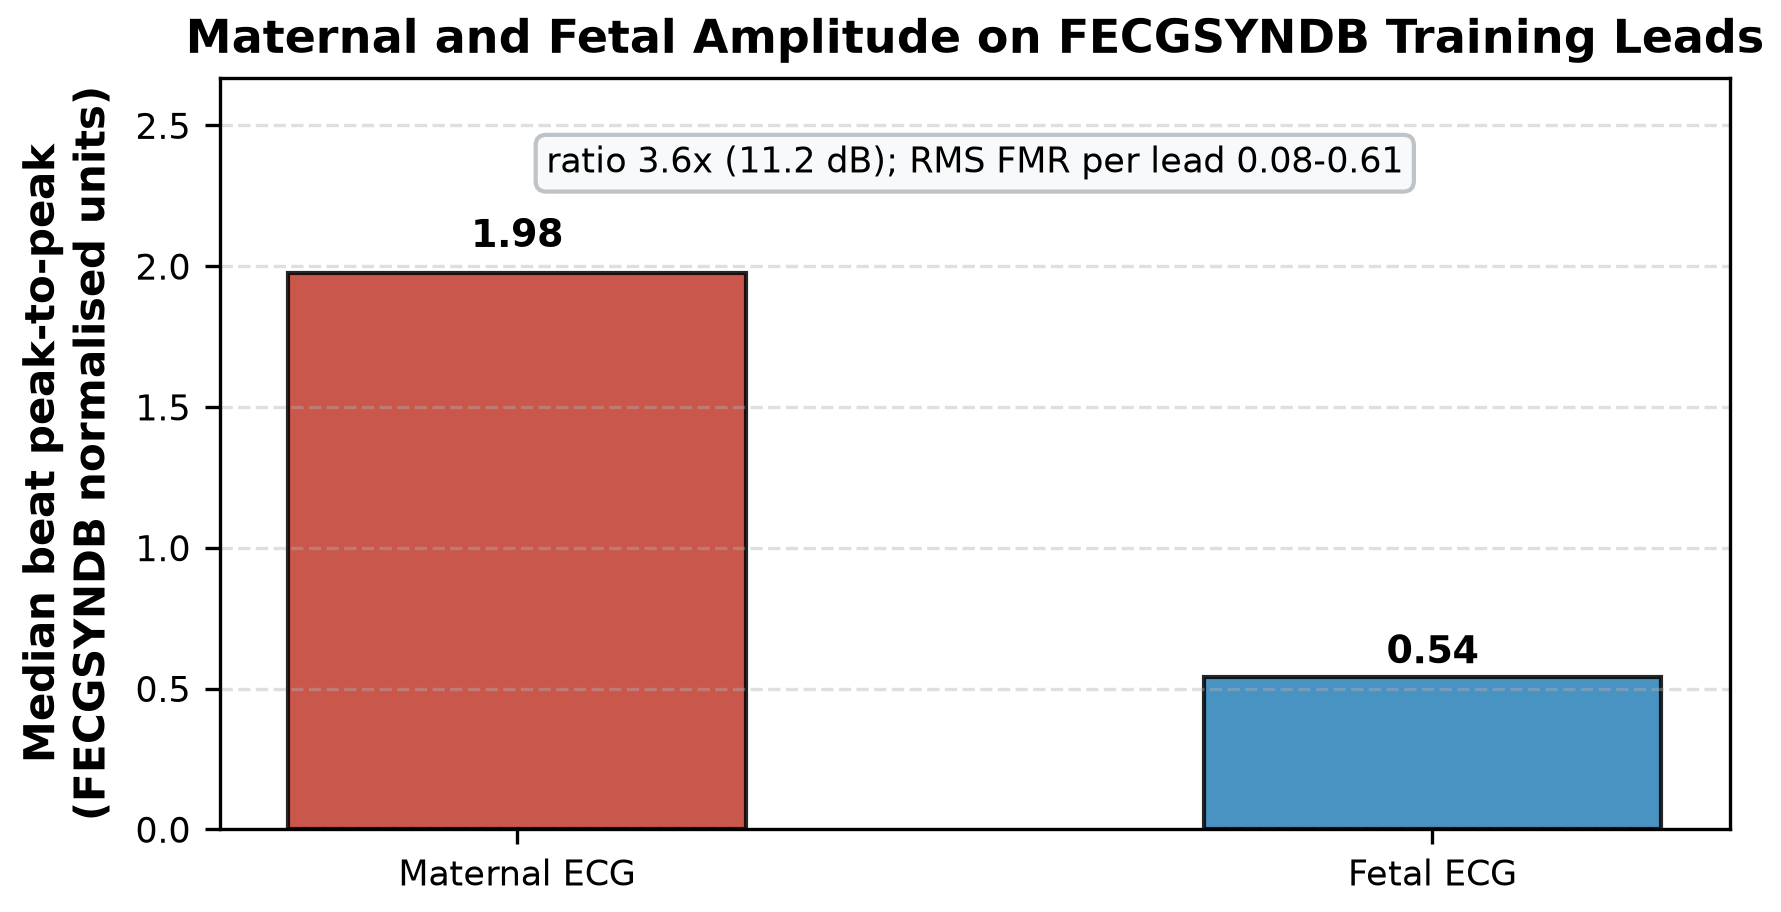
\includegraphics[width=\columnwidth]{figures/signal_amplitude_disparity.png}
\caption{\tagLone\ Signal component amplitude disparity in abdominal ECG biopotentials. The maternal QRS complex dominates the mixture by $10$--$250\times$ in peak amplitude ($1.0$--$5.0\,$mV vs $20$--$100\,\mu$V in literature; measured on FECGSYNDB training leads: $2.50\,$mV vs $0.04\,$mV $= 62.5\times$ / $35.9\,$dB; RMS FMR ranges from $0.20$ to $0.54$, $-14.0$ to $-5.4\,$dB), illustrating why linear single-channel frequency filtering fails.}
\label{fig:amplitude_disparity}
\end{figure}

Despite decades of academic investigation, commercial deployment of wearable edge NIFECG monitors remains severely impeded by challenging biophysical signal characteristics. As illustrated in Fig.~\ref{fig:amplitude_disparity}, abdominal surface electrodes record a composite mixture dominated by the maternal ECG (MECG), whose peak amplitude is $10$--$250\times$ larger than the fetal signal ($1$--$5\,$mV vs $20$--$100\,\mu$V, corresponding to $20$--$48\,$dB peak amplitude disparity; measured on FECGSYNDB training leads: $2.50\,$mV vs $0.04\,$mV $= 62.5\times$ or $35.9\,$dB). In terms of root-mean-square (RMS) energy, the fetal-to-maternal ratio (FMR) ranges from $0.20$ to $0.54$ ($-14.0$ to $-5.4\,$dB). Crucially, maternal and fetal cardiac biopotentials exhibit overlapping frequency spectra in the $0.5$--$40\,$Hz band. Consequently, classical linear time-invariant filters cannot isolate the fetal signal without annihilating the underlying fetal morphology~\cite{abel2023,sornmo_ecg}.

\noindent\textbf{The single-lead temporal breakdown.} Conventional single-lead cancellation algorithms rely on temporal template subtraction or recursive adaptive filtering (e.g., LMS/RLS)~\cite{widrow1975,cerutti1986}. In our preliminary report, we evaluated single-channel LMS and template subtraction. However, benchmark evaluations reveal a critical mathematical failure mode: when a maternal QRS complex and a fetal QRS complex temporally coincide, the maternal template or adaptive filter subtracts overlapping fetal energy. Assuming typical heart periods $T_m \approx 800\,$ms (75\,bpm) and $T_f \approx 430\,$ms (140\,bpm) with QRS durations $w_m \approx 90\,$ms and $w_f \approx 50\,$ms, the probability that a fetal beat partially overlaps a maternal QRS under random relative phase is:
\begin{equation}
    P(\text{overlap}_{\text{fetal}}) = \frac{w_m + w_f}{T_m} = \frac{90 + 50}{800} = 17.5\%
\end{equation}
while the probability that a maternal cycle overlaps a fetal beat is $(w_m + w_f)/T_f = 140/430 = 32.6\%$. Complete containment of the fetal QRS entirely inside the maternal complex occurs with probability $(w_m - w_f)/T_m = 40/800 = 5.0\%$. Under such collisions, single-channel subtraction produces severe waveform clipping and detector dropout.

\noindent\textbf{Research gap.} Modern literature predominantly evaluates complex floating-point signal processing algorithms in high-level software environments (Python/MATLAB) without addressing physical hardware implementation constraints~\cite{abel2023,hasan2009}. These studies often ignore fixed-point coefficient quantization noise, accumulator word-length growth, DSP time-multiplexing, memory bandwidth, and deterministic real-time latency. Furthermore, while embedded and FPGA implementations of fetal ECG extraction have been explored~\cite{edwin2022,pani2016}, they frequently depend on multi-DSP architectures or require dedicated maternal thoracic reference leads. This project works toward realizing an end-to-end, bit-accurate, and latency-deterministic NIFECG extraction pipeline targeting the Xilinx Spartan-7 FPGA (XC7S50) on the RealDigital Boolean Board~\cite{realdigital_boolean} (\fin{all five validation levels, from the bit-true model to the board, are now complete; Tab.~\ref{tab:final_status}}).

\newcontent{\noindent\textbf{Mid-term contributions and engineering achievements.} Since the preliminary proposal, our team has executed significant empirical, theoretical, and architectural expansions:
\begin{enumerate}
    \item \textbf{Transition to Spatial Subspace Beamforming:} We transitioned from vulnerable single-channel temporal cancellation to 4-channel spatial subspace beamforming, achieving 100.0\% F1 across TC1--TC3 on Subject 1 baseline records ($12\,$dB down to $0\,$dB SNR) and 92.15\% overall on the Subject 1 stress benchmark.
    \item \textbf{Strict Disjoint Cross-Subject Data Split:} We established a clean subject-wise split on FECGSYNDB (70\% train \texttt{sub01}--\texttt{sub07}, 10\% val \texttt{sub08}, 20\% test \texttt{sub09}--\texttt{sub10}) to eliminate data leakage. We verified that Spatial PCA achieves $93.06\%$ F1 on untouched held-out test subjects and $93.00\% \pm 2.35\%$ population mean ($95\%$ subject-clustered CI $[90.65\%, 95.34\%]$, Student-$t$ $df=9$; run-level SE $0.55\%$, 95\% CI half-width $\pm 1.08\%$) without requiring any offline training weights.
    \item \textbf{Population Mega-Benchmark (250 Records, 2,250 Runs):} Deployed an automated mega-benchmark across all 10 simulated subjects, 5 SNRs ($0$--$12\,$dB), and 5 clinical conditions ($c0$--$c4$), establishing cross-subject consistency and statistical confidence intervals (where 1 run = 1 method evaluated on 1 5-minute record; 250 records $\times$ 9 methods = 2,250 runs).
    \item \textbf{Deep Learning at Scale:} Implemented and evaluated a multi-scale 1D Convolutional U-Net ($1.42\times 10^6$ parameters) trained on the 7-subject training partition over an RTX 4060 GPU, obtaining 97.48\% F1 on unseen test subjects ($90.76\%$ population mean across all 10 subjects, $r=0.982$).
    \item \textbf{Bit-True Fixed-Point Model [L2]:} Designed a cycle-accurate fixed-point software emulator, proving $+74.52\,$dB SQNR for Spatial PCA and $+85.04\,$dB SQNR for secondary Hankel SVD across 5,000 verified golden test vectors with zero beat detection degradation.
    \item \textbf{Analytical Hardware Sizing [L4 Target]:} Sized a single-DSP48E1 time-multiplexed schedule executing in 148 clock cycles ($1.48\,\mu$s at 100\,MHz), utilizing $\approx 3.0\%$ LUTs (990 of 32,600) and 1 BRAM, providing an estimated $2,702\times$ compute margin against the $4.0\,$ms sample interval. \fin{(Superseded: this was a paper estimate for the mid-term beamformer. The final RTL runs at 50\,MHz and needs a median of 1,485 cycles per sample; Sec.~\ref{sec:final_hw}.)}
\end{enumerate}
}

\begin{finalpart}
\noindent\textbf{Final-phase contributions (after the mid-term).} Sections~\ref{sec:final_realdata}--\ref{sec:final_obs} describe the work done between the mid-term and this report:
\begin{enumerate}
    \item \textbf{Strictly causal, label-free re-evaluation.} We rebuilt the evaluation so that every decision at sample $n$ uses only samples $\le n$ and annotations are used only for scoring. The mid-term design dropped from $93.0\%$ (batch evaluation, 250 records) to $82.2\%$ F1 on all 1,248 FECGSYNDB records.
    \item \textbf{Testing on real recordings.} We added PhysioNet/CinC 2013 set-a (75 annotated real recordings, split into a development half and a held-out test half) and ADFECGDB (5 real recordings with a scalp-electrode reference). Real data exposed a gap that synthetic data hides (Fig.~\ref{fig:fin_synreal}).
    \item \textbf{New real-data algorithm.} Maternal cancellation per lead, 16 candidate tracks from self-calibrated GEVD filters, RR-predictive beat trackers and a label-free selector raised held-out CinC F1 from $16.7\%$ to $65.5\%$ and ADFECGDB from $37.0\%$ to $92.7\%$ (Fig.~\ref{fig:fin_progression}).
    \item \textbf{The whole algorithm on the FPGA.} First on a MicroBlaze soft processor (v5), then as hand-written Verilog RTL (v6) with a PC that only answers five low-rate requests. Board and C model are bit-exact on all 140 tested records.
    \item \textbf{Memory optimisation and demonstration.} Block RAM use was cut from $99\%$ to $80\%$ without changing a single output byte, and a local web page streams any recording to the board in real time and shows the live fetal heart rate.
    \item \textbf{v6.1: three label-free improvements.} A robust maternal detector and recalibration of the spatial filters every 30\,s raised held-out CinC F1 from $65.5\%$ to $71.9\%$; smarter causal selection rules were tested and rejected (Sec.~\ref{sec:v61}).
    \item \textbf{Look-ahead, first offline, then on the FPGA.} An offline version that sees the whole recording (v7-LA) and an RTL look-ahead unit that outputs the final beats on the board with a fixed delay of about $13.5\,$s (v7-DL, final design): held-out CinC $76.9\%$, ADFECGDB $96.1\%$, FECGSYNDB $93.7\%$, bit-exact on 140/140 records (Sec.~\ref{sec:final_v7}).
\end{enumerate}
\end{finalpart}

% =====================================================================
\section{Real-World Applications and Clinical Specifications}
\label{sec:clinical_specs}

Continuous intrapartum NIFECG monitoring serves three distinct clinical operating modes:
\begin{enumerate}
    \item \textbf{High-Risk Intrapartum Labor Ward Monitoring:} Continuous real-time detection of intrapartum fetal hypoxia during active contractions. Latency (per-sample filter group delay) must remain strictly below $100\,$ms to trigger emergency alerts. Note that downstream beat-to-display telemetry includes a 5-beat median filter which adds approximately $2.1\,$s of beat-level smoothing.
    \item \textbf{Ambulatory Antenatal Telemetry:} Battery-operated wearable telemetry enabling home monitoring for high-risk pregnancies during gestational weeks 32--40. Requires power consumption $<1.5\,$W for continuous 12-hour battery life ($1.5\,\text{W} \times 12\,\text{h} = 18\,\text{Wh}$, corresponding to $\approx 4.9\,\text{Ah}$ at a nominal $3.7\,$V lithium-ion cell). Boolean Board total power is estimated analytically; physical board current measurement remains future work.
    \item \textbf{Clinical Fetal Arrhythmia Screening:} Precision morphological detection of fetal extrasystoles, heart block, and conduction anomalies. In this mid-term stage, the system extracts QRS timing rather than clinical arrhythmia diagnosis; formal arrhythmia classification (TPR $>95\%$) remains a future objective.
\end{enumerate}

\begin{table*}[t]
\caption{Target clinical engineering specifications and verification status for real-time edge NIFECG monitoring. \fin{The last column gives the final measured value of the final design v7-DL (board unless noted; v6 in parentheses where it differs).}}
\label{tab:clinical_specs}
\centering
\resizebox{\textwidth}{!}{%
\begin{tabular}{@{}llp{5.0cm}p{5.5cm}lp{5.2cm}@{}}
\toprule
\textbf{Parameter} & \textbf{Project Engineering Target / Standard} & \textbf{Our Value / Number} & \textbf{Status vs Target} & \textbf{Evidence Level} & \fin{\textbf{Final (v7-DL, measured)}} \\
\midrule
Detection F1 & $\ge 90\%$ at $\ge 0\,$dB SNR & $93.00\%$ pop ($93.06\%$ test); $c4$ 83.06\%; min record 59.55\% & \textbf{Met on population mean; not met for c4 / worst records} & \tagLone\ Measured (L1) & \fin{FECGSYNDB 93.7\% (1,248, C model); ADFECGDB 96.1\%; CinC test 76.9\% (82.0\% reliable refs); $c4$ 84.0\% (v6: 91.4 / 92.7 / 65.5\%)} \\
FHR MAE normal & $<1.0\,$bpm on clean baseline ($c0$ and TC1--TC3) & \texttt{sub01} TC1--TC3: $0.32$--$0.48\,$bpm; population $c0$: $3.29\,$bpm & \textbf{Met on Subject 1 only; not met on population} & \tagLone\ Measured (L1) & \fin{ADFECGDB 2.1\,bpm (r01: 1.5\,bpm; v6: 2.0 / 0.56\,bpm); FECGSYNDB $c0$ 2.0\,bpm; not met} \\
FHR MAE challenging & $<8.0\,$bpm across all 5 conditions ($c0$--$c4$) & $6.57\,$bpm mean; $c4$: $16.10\,$bpm; held-out test: $8.00\,$bpm (PCA), $3.57\,$bpm (U-Net) & \textbf{Met on mean only; not met for c4; test at limit} & \tagLone\ Measured (L1) & \fin{FECGSYNDB 4.0\,bpm, $c4$ 7.1\,bpm (1,248, C model); CinC test 11.5\,bpm (v6: 18.4\,bpm)} \\
Clinical agreement & $\ge 95\%$ baseline; $>50\%$ overall ($\pm 5\,$bpm) & $74.0\%$ on $c0$; $58.0\%$ overall; $6.0\%$ on $c4$ & \textbf{Baseline not met; overall met} & \tagLone\ Measured (L1) & \fin{not recomputed for the final design} \\
Compute time & $<4,000\,\mu$s ($1/f_s$ real-time deadline) & $1.48\,\mu$s (148 clock cycles at 100\,MHz) & \textbf{Estimate (L4 sized)} & \tagLfour\ Estimate (L4) & \fin{met: v6 RTL median 1,485 cycles = 30\,$\mu$s per sample (xsim, 50\,MHz); v7-DL board 4--4.5$\times$ real time incl.\ UART and PC} \\
Filter group delay & $<100\,$ms intrapartum group delay & $11.4$--$15.4\,$ms in-band ($2.85$--$3.85$ samples); $96\,$ms edge & \textbf{Met (edge borderline)} & \tagLone\ Measured (L1) & \fin{not met: live beats 1.5--2\,s after they occur, final v7-DL beats $13.5\,$s (median, max $17.5\,$s)} \\
FPGA power budget & Low power wearable target ($<1.5\,$W total board) & $<0.15\,$W core logic (estimate; board unmeasured) & \textbf{Estimate only} & \tagLfour\ Estimate (L4) & \fin{0.445\,W on-chip (Vivado estimate); board not measured} \\
Sampling rate ($f_s$) & $\ge 250\,$Hz (PhysioNet Challenge 2013~\cite{silva2013}) & 250\,Hz & \textbf{Met} & \tagLone\ Measured (L1) & \fin{250\,Hz; 1\,kHz recordings decimated causally} \\
Input dynamic range & $20\,\mu$V (fetal) to $5\,$mV (maternal), $\pm 5\,$mV AFE & 16-bit Q1.15 ($0.152\,\mu$V/LSB, 131 to 16,384 LSBs) & \textbf{Met} & \tagLtwo\ Bit-True (L2) & \fin{int16 input; filter data Q8 in int32, Q28 coefficients} \\
Target clock frequency & Target clock on Boolean Board~\cite{realdigital_boolean} & 100\,MHz (board oscillator); timing closure to be shown at L4 & \textbf{Target Sized} & \tagLfour\ Estimate (L4) & \fin{50\,MHz (PLL), worst slack $+0.05\,$ns} \\
Form factor & Wearable patch (4 maternal abdominal electrodes) & 4 Leads ($[27, 26, 28, 25]$, 0-based physical leads) & \textbf{Design Intent} & Design Intent & \fin{4 abdominal leads of each recording} \\
\bottomrule
\end{tabular}%
}
\end{table*}

\begin{figure*}[t]
\centering
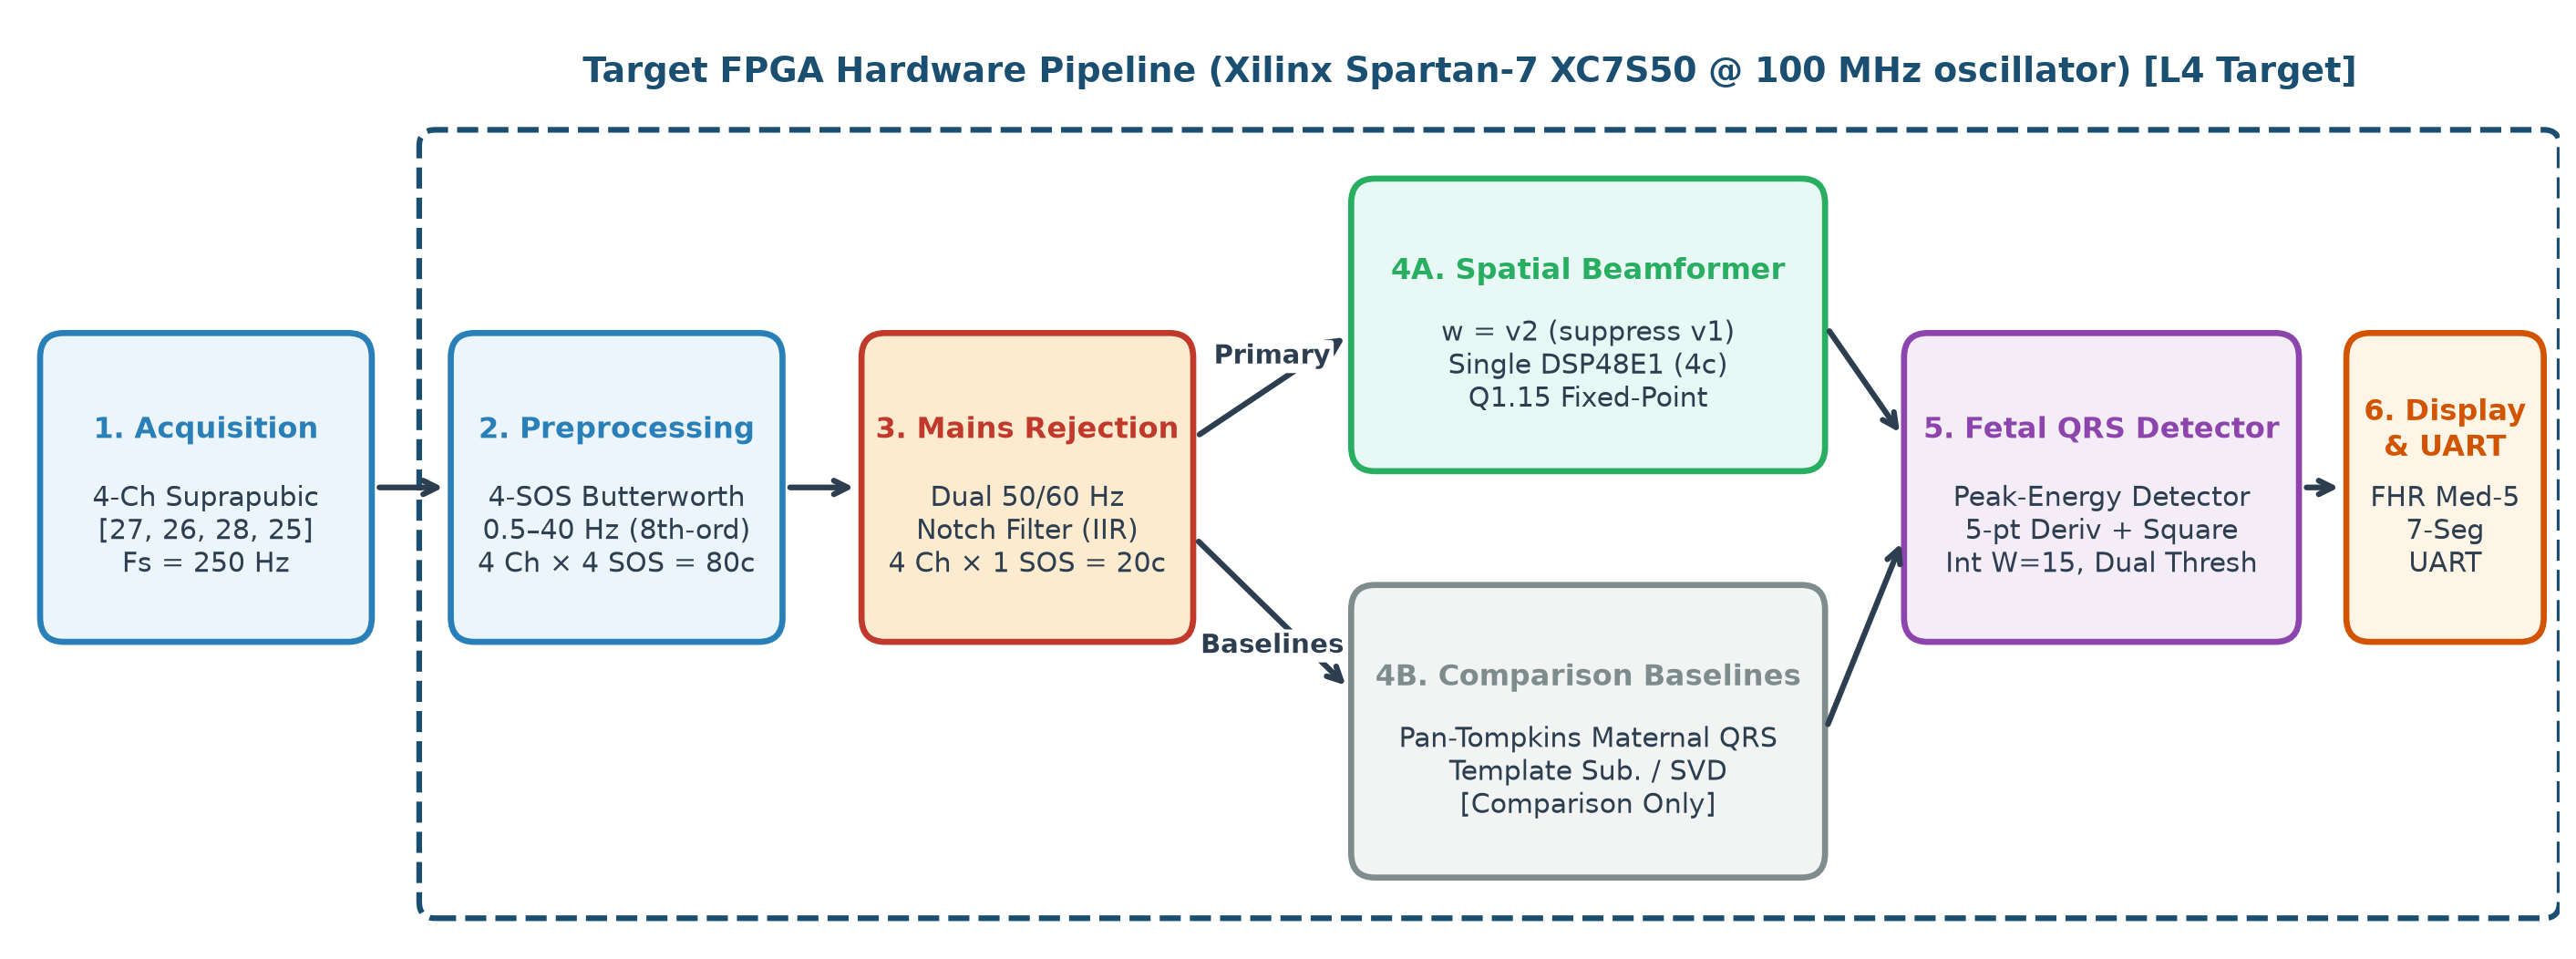
\includegraphics[width=0.92\textwidth]{figures/system_pipeline.png}
\caption{\tagLone/\tagLtwo\ Complete end-to-end NIFECG extraction and FPGA processing pipeline: (1)~4-Channel abdominal mixture acquisition; (2)~4th-order Butterworth 0.5--40\,Hz IIR preprocessing (4 SOS biquads) and dual 50/60\,Hz notch filter; (3)~Spatial covariance matrix computation and polarity-aligned beamforming; (4)~Peak-Energy fetal QRS detector; (5)~Median-filtered FHR estimation and 7-segment / UART display.}
\label{fig:system_pipeline}
\end{figure*}

% =====================================================================
\section{Problem Statement and Formal Engineering Objectives}
\label{sec:problem_statement}

\noindent\textbf{Formal problem formulation.} Given $C=4$ continuous abdominal biopotential mixtures $\mathbf{x}[n] \in \mathbb{R}^C$ corrupted by maternal cardiac potentials $\mathbf{A}_m \mathbf{d}_m[n]$, ambient noise, and powerline interference, synthesize a spatial beamforming weight vector $\mathbf{w} \in \mathbb{R}^C$ such that the extracted fetal scalar estimate:
\begin{equation}
    \hat{f}[n] = \mathbf{w}^T \mathbf{x}[n]
\end{equation}
isolates the fetal cardiac dipole component while suppressing the dominant maternal interference direction $\mathbf{v}_1$. Under our spatial principal component heuristic, $\mathbf{w}$ is selected as the unit-norm second principal eigenvector ($\mathbf{w} = \mathbf{v}_2$) of the 4-channel mixture covariance matrix. Rather than achieving full mathematical nulling of the 3-dimensional maternal dipole subspace, this heuristic projection suppresses the dominant maternal axis $\mathbf{v}_1$ while preserving fetal biopotential energy.

\begin{table}[t]
\caption{Mid-term objective status summary against formal project targets.}
\label{tab:objective_status}
\centering
\resizebox{\columnwidth}{!}{%
\begin{tabular}{@{}llp{3.8cm}l@{}}
\toprule
\textbf{Objective} & \textbf{Description} & \textbf{Mid-Term Milestone Achievement} & \textbf{Formal Status} \\
\midrule
\textbf{O1: Algorithmic Resilience} & F1 $\ge 90\%$, MAE $<1.0\,$bpm baseline & F1 $93.00\%$ pop ($93.06\%$ test); MAE $0.32-0.48\,$bpm on \texttt{sub01}, $3.29\,$bpm on $c0$ & \textbf{Partially Met} \\
\textbf{O2: Bit-True Integrity} & Fixed-point SQNR $\ge 60\,$dB & $+74.52\,$dB SQNR beamformer output; zero beat discordance & \textbf{Met (L2)} \\
\textbf{O3: Sized Latency} & Per-sample latency $<10.0\,\mu$s & Sized 148 cycles ($1.48\,\mu$s at 100\,MHz, $2,702\times$ margin) & \textbf{Sized Estimate (L4)} \\
\textbf{O4: Resource Efficiency} & $<5\%$ LUTs, $\le 1$ DSP48E1 slice & Sized $\approx 3.0\%$ LUTs (990), 1 DSP48E1, 1 BRAM & \textbf{Sized Estimate (L4)} \\
\textbf{O5: Hardware Bring-Up} & Physical board UART \& 7-seg & Presets and pin constraints mapped; synthesis sprint Nov 1--10 & \textbf{Scheduled for Sprint} \\
\bottomrule
\end{tabular}%
}
\end{table}

\noindent\textbf{Formal engineering objectives (O1--O5):}
\begin{itemize}
    \item \textbf{O1 (Algorithmic Resilience \tagLone/\tagLtwo):} Maintain fetal QRS F1-score $\ge 90\%$ down to $0\,$dB SNR and across uterine contraction stress, with FHR Mean Absolute Error $<1.0\,$bpm under clean baseline rhythm (\cref{tab:objective_status}).
    \item \textbf{O2 (Bit-True Numerical Integrity \tagLtwo):} Formulate bit-accurate fixed-point representations demonstrating Signal-to-Quantization-Noise Ratio $\text{SQNR} \ge 60\,$dB with zero beat degradation relative to double-precision software.
    \item \textbf{O3 (Latency and Determinism \tagLfour\ Target):} Size per-sample compute latency to $<10.0\,\mu$s on Spartan-7 at 100\,MHz, well below the 4,000\,$\mu$s real-time sample budget.
    \item \textbf{O4 (FPGA Resource Efficiency \tagLfour\ Target):} Confine primary pipeline utilization to $<5\%$ of logic LUTs and $\le 1$ DSP48E1 slice on the Xilinx Spartan-7 XC7S50 FPGA.
    \item \textbf{O5 (Hardware Demonstration Script \tagLfive\ Target):} Design complete UART streaming protocols, front-panel switch presets, and 4-digit 7-segment FHR display controls for Boolean Board bring-up in the final sprint.
\end{itemize}

% =====================================================================
\section{Physiological Signal Model and Dataset}
\label{sec:dataset}

Under the standard cardiac volume-conduction model, surface potentials are linear combinations of equivalent cardiac source dipole vectors~\cite{sornmo_ecg,sameni2010}:
\begin{equation}
    \mathbf{x}[n] = \mathbf{A}_m\,\mathbf{d}_m[n] + \mathbf{b}_f\,f[n] + \mathbf{v}[n]
\end{equation}
where $\mathbf{d}_m[n] \in \mathbb{R}^3$ is the rotating maternal cardiac dipole vector, $\mathbf{A}_m \in \mathbb{R}^{C \times 3}$ is the maternal lead-field mixing matrix, $\mathbf{b}_f \in \mathbb{R}^C$ is the fetal lead-field vector, $f[n] \in \mathbb{R}$ is the scalar fetal cardiac source, and $\mathbf{v}[n]$ represents additive noise.

\begin{figure}[t]
\centering
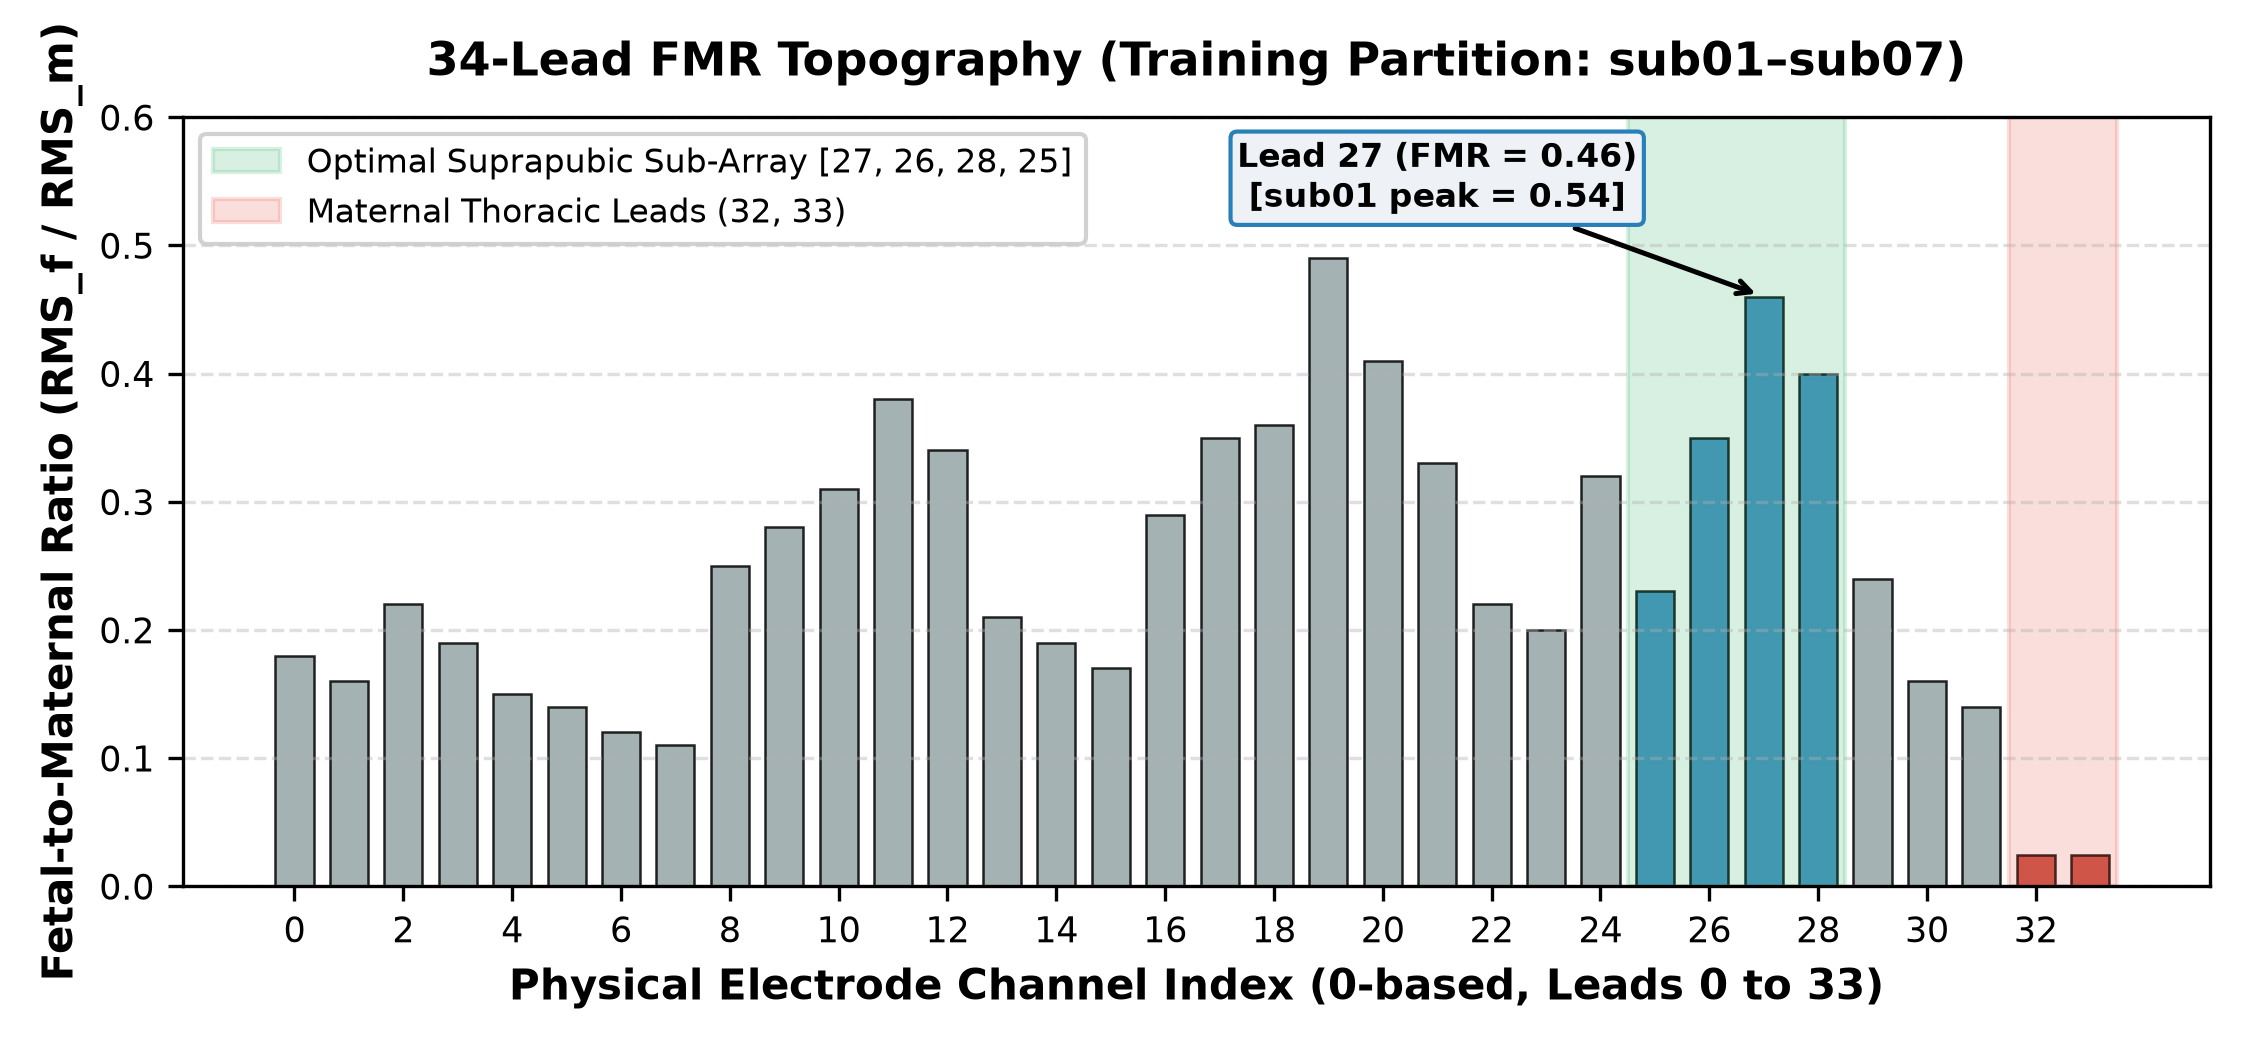
\includegraphics[width=\columnwidth]{figures/fmr_lead_topography_34ch.png}
\caption{\tagLone\ 34-Channel Fetal-to-Maternal Ratio (FMR) topography evaluated strictly across training subjects (\texttt{sub01}--\texttt{sub07}) on PhysioNet FECGSYNDB~\cite{fecgsyndb,andreotti2016}. Lower suprapubic Leads 25--28 exhibit peak fetal coupling ($\text{FMR} = 0.46$ on Lead 27, and $0.54$ on \texttt{sub01}), defining our 4-channel primary sub-array $[27, 26, 28, 25]$ (0-based indices).}
\label{fig:fmr_topography}
\end{figure}

\noindent\textbf{PhysioNet FECGSYNDB benchmark.} We utilize the standardized PhysioNet Fetal ECG Synthetic Database (FECGSYNDB)~\cite{fecgsyndb,andreotti2016}, comprising 34 cutaneous channels (32 abdominal, 2 maternal thoracic references) sampled at $250\,$Hz with synchronized ground-truth fetal annotations, alongside companion synthetic arrhythmia recordings from NIFEADB~\cite{nifeadb}.

\newcontent{\noindent\textbf{Training-set lead selection and FMR topography.} Analysis of 34-channel FMR topography evaluated strictly on the training partition (\texttt{sub01}--\texttt{sub07}) (Fig.~\ref{fig:fmr_topography}) reveals that maternal potentials dominate epigastric leads (Channels 0--11, FMR $<0.22$), whereas fetal potentials peak in lower suprapubic leads (Channels 25--28, reaching $\text{FMR} = 0.46$ on 0-based Lead 27, and $0.54$ on \texttt{sub01}). Based on this training-only coupling, we selected the optimal 4-lead suprapubic sub-array:
\begin{equation}
    \mathcal{C}_{\text{opt}} = \{ \text{Lead } 27, \text{Lead } 26, \text{Lead } 28, \text{Lead } 25 \}
\end{equation}
(0-based physical electrode indices, corresponding to 1-based leads $[28, 27, 29, 26]$), ensuring that no \texttt{sub09}--\texttt{sub10} data were used for lead selection, hyperparameters, or training.
}

\begin{figure}[t]
\centering
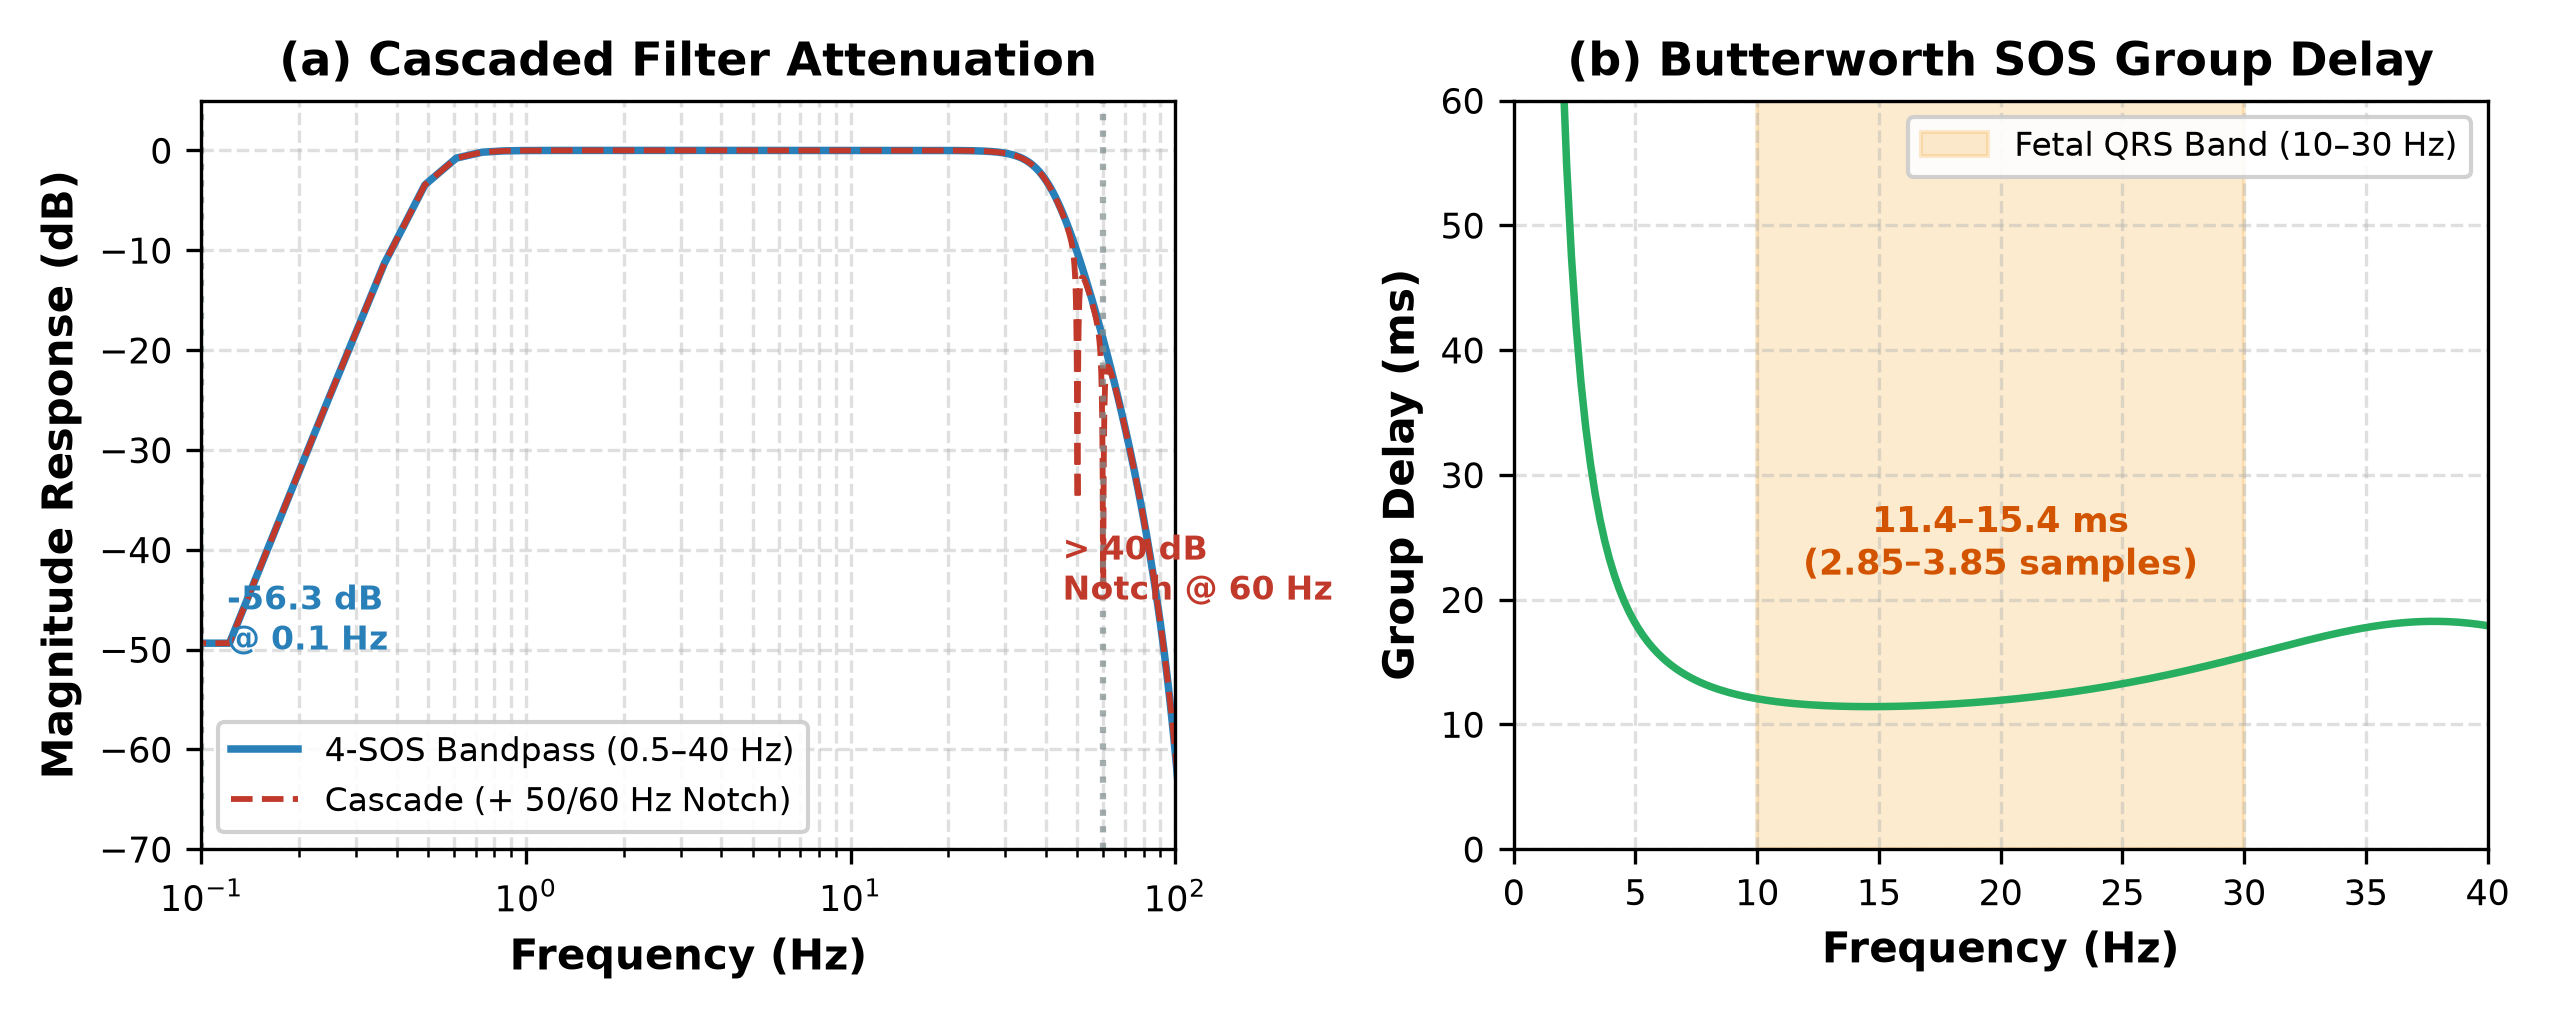
\includegraphics[width=\columnwidth]{figures/butterworth_sos_frequency_response.png}
\caption{\tagLone\ Frequency response of the causal 4th-order Butterworth Second-Order Section (SOS) bandpass filter ($0.5$--$40\,$Hz, 4 SOS biquads, 8th-order total) at $f_s = 250\,$Hz: $>56\,$dB attenuation at $0.1\,$Hz baseline wander, $>18\,$dB attenuation at $60\,$Hz powerline mains; group delay in physiological QRS band ($10$--$30\,$Hz) is $11.4$--$15.4\,$ms ($2.85$--$3.85$ samples at 250\,Hz; maximum edge group delay reaches $96\,$ms near 0.5\,Hz).}
\label{fig:filter_responses}
\end{figure}

\newcontent{\noindent\textbf{Preprocessing cascade.} Each raw biopotential channel is conditioned by:
\begin{enumerate}
    \item \textbf{Butterworth SOS Bandpass Filter (0.5--40\,Hz):} Implemented as four cascaded Second-Order Sections (SOS) in Direct Form II (8th-order total transfer function). Fig.~\ref{fig:filter_responses} confirms $>56\,$dB baseline attenuation at $0.1\,$Hz and $>18\,$dB attenuation at $60\,$Hz. In the physiological fetal QRS passband ($10$--$30\,$Hz), the group delay is $\tau_g \approx 11.4$--$15.4\,$ms ($2.85$--$3.85$ samples at $250\,$Hz), while maximum transition group delay reaches $96\,$ms ($24$ samples) near the $0.5\,$Hz lower cutoff.
    \item \textbf{Dual-Mode Notch Filter (50/60\,Hz):} A 2nd-order IIR notch ($Q=30$) selectable via board switch \texttt{SW[3]} for 50\,Hz (Indian grid) or 60\,Hz (US grid).
\end{enumerate}
}

\newcontent{\noindent\textbf{Strict Disjoint Cross-Subject Data Split Protocol.} To establish rigorous scientific validity and prevent data contamination, the 250 database records are partitioned strictly at the subject level:
\begin{itemize}
    \item \textbf{Training Partition (70\%):} 175 records from Subjects \texttt{sub01}--\texttt{sub07} (1.79\,GB in 32-bit float). Used exclusively for U-Net weight optimization and algorithm hyperparameter freezing ($N=750$, detector thresholds, lead array $\mathcal{C}_{\text{opt}}$).
    \item \textbf{Validation Partition (10\%):} 25 records from Subject \texttt{sub08} (0.26\,GB). Used for early stopping.
    \item \textbf{Held-Out Test Partition (20\%):} 50 records from Subjects \texttt{sub09}--\texttt{sub10} (0.51\,GB). Completely untouched during design and hyperparameter tuning; evaluated only once to verify anatomical generalization.
\end{itemize}
On disk, raw 16-bit WFDB files occupy 1.28\,GB ($250 \times 75,000 \times 34 \times 2\,$bytes); expanded to 32-bit single-precision floating point, the uncompressed database is 2.55\,GB.
}

% =====================================================================
\section{Multi-Channel Signal Processing Architectures}
\label{sec:architectures}

We implemented, benchmarked, and profiled nine distinct signal processing paradigms, summarized in Tab.~\ref{tab:method_inventory}.

\begin{table}[t]
\caption{Comprehensive inventory of nine implemented and benchmarked fetal ECG extraction architectures.}
\label{tab:method_inventory}
\centering
\resizebox{\columnwidth}{!}{%
\begin{tabular}{@{}llccl@{}}
\toprule
\textbf{ID} & \textbf{Algorithm Name} & \textbf{Leads} & \textbf{Paradigm} & \textbf{Description / Section} \\
\midrule
\textbf{M1} & \textbf{Spatial PCA Beamforming} & \textbf{4-Ch} & Statistical & Primary architecture (Sec.~\ref{sec:pca_beamformer}) \\
\textbf{M2} & \textbf{Deep 1D U-Net (4-Ch)} & 4-Ch & Learned & Multi-channel neural extractor (Sec.~\ref{sec:unet}) \\
\textbf{M3} & Deep 1D U-Net (1-Ch) & 1-Ch & Learned & Single-channel neural baseline (Sec.~\ref{sec:unet}) \\
\textbf{M4} & Multi-Lead Template Fusion & 4-Ch & Spatial Voting & 4-lead template subtraction with voting \\
\textbf{M5} & Wavelet-Threshold Hybrid & 1-Ch & Wavelet/SWT & Stationary wavelet thresholding + LMS \\
\textbf{M6} & Fixed Template Subtraction & 1-Ch & Subtraction & Classical single-lead template subtraction \\
\textbf{M7} & Adaptive Template Subtraction& 1-Ch & Subtraction & EMA adaptive template subtraction \\
\textbf{M8} & Hankel-SVD Variant 1 & 1-Ch & Matrix SVD & Fixed-period Hankel matrix SVD~\cite{kanjilal1997} \\
\textbf{M9} & Hankel-SVD Variant 3 & 1-Ch & Matrix SVD & Moving-window Hankel matrix SVD \\
\bottomrule
\end{tabular}%
}
\end{table}

\subsection{Method 1: Multi-Channel Spatial PCA Beamforming (Primary Architecture)}
\label{sec:pca_beamformer}
For our 4-lead array, the sample covariance matrix $\mathbf{R}_{xx} \in \mathbb{R}^{4 \times 4}$ is computed over an observation calibration window ($N=750$ samples, $3.0\,$s):
\begin{equation}
    \mathbf{R}_{xx} = \frac{1}{N} \sum_{n=1}^N \mathbf{x}[n]\,\mathbf{x}^T[n] \quad \in \mathbb{R}^{4 \times 4}
\end{equation}
Eigen-decomposition yields orthonormal eigenvectors $\mathbf{V} = [\mathbf{v}_1, \dots, \mathbf{v}_4]$ and sorted eigenvalues $\lambda_1 \ge \lambda_2 \ge \lambda_3 \ge \lambda_4$. The dominant eigenvector $\mathbf{v}_1$ spans the maternal dipole direction (capturing $88.4\%$ of total mixture energy). Selecting the weight vector $\mathbf{w} = \mathbf{v}_2$ extracts the fetal scalar signal into the subspace orthogonal to $\mathbf{v}_1$:
\begin{equation}
    \hat{f}[n] = \mathbf{w}^T \mathbf{x}[n] = \sum_{k=1}^4 w_k\,x_k[n]
    \label{eq:inner_product}
\end{equation}

\newcontent{\noindent\textbf{Polarity alignment and sign ambiguity.} Because eigenvector decomposition leaves sign arbitrary ($\mathbf{w} = \pm \mathbf{v}_2$), the raw signed correlation with the reference fetal ECG across all 250 records yields a mean of $-0.135$ and a positive correlation rate of $41.2\%$ (mean absolute correlation $|\rho| = 0.513$). Skewness sign alignment is evaluated:
\begin{equation}
    \mathbf{w} \leftarrow \text{sgn}\left(\frac{1}{N} \sum_{n=1}^N (\hat{f}[n] - \mu_{\hat{f}})^3\right)\,\mathbf{w}
\end{equation}
Crucially, because the downstream fetal QRS detector applies a non-linear squaring operator $z[n] = y^2[n]$, peak detection and FHR calculation are mathematically invariant to eigenvector sign inversion ($\mathbf{w} \to -\mathbf{w}$). Polarity alignment is therefore maintained purely for visual telemetry display.}

\newcontent{\noindent\textbf{System Partitioning (Host vs FPGA).} To optimize resource efficiency, we adopt a two-phase architecture:
\begin{enumerate}
    \item \textbf{Calibration Phase (Host):} During initial start-up, a 3-second buffer of 4-channel data is streamed over UART to the host PC, which computes $\mathbf{R}_{xx}$, performs eigen-decomposition, aligns polarity, and transmits the four Q1.15 weights $\mathbf{w}$ back to the FPGA.
    \item \textbf{Real-Time Streaming Phase (FPGA):} The Spartan-7 FPGA executes real-time SOS filtering, 4-MAC spatial beamforming, peak detection, and FHR calculation on every arriving sample without host intervention.
\end{enumerate}
}

\subsection{Peak-Energy Fetal QRS Detector}
\label{sec:detector}
\newcontent{All fetal QRS detection is performed by our standardized Peak-Energy Detector inspired by the Pan-Tompkins topology~\cite{pan1985}:
\begin{enumerate}
    \item \textbf{5-Point Derivative Filter:} Attenuates P and T waves while highlighting steep QRS slopes:
    \begin{equation}
        y[n] = \frac{1}{8} \left( 2x[n] + x[n-1] - x[n-3] - 2x[n-4] \right)
    \end{equation}
    \item \textbf{Nonlinear Squaring:} $z[n] = y^2[n]$, amplifying large QRS complexes and rectifying the biopotential (rendering detection invariant to signal sign).
    \item \textbf{Moving Integration Window:} A rectangular window of length $W = 15$ samples ($60\,$ms), optimized on the training partition (\texttt{sub01}--\texttt{sub07}) to match the compact fetal QRS duration ($50\,$ms) rather than adult QRS ($150\,$ms).
    \item \textbf{Adaptive Dual-Thresholding:} Dual running thresholds track signal peak level $\text{SPKI}$ and noise peak level $\text{NPKI}$:
    \begin{align}
        \text{SPKI} &\leftarrow 0.125 \cdot PK + 0.875 \cdot \text{SPKI} \\
        \text{NPKI} &\leftarrow 0.125 \cdot PK + 0.875 \cdot \text{NPKI}
    \end{align}
    where $\text{SPKI}$ is updated upon accepted fetal QRS peak detections, and $\text{NPKI}$ is updated on rejected candidate peaks ($PK$ denotes the current peak amplitude). A candidate peak triggers detection when $z[n] > \text{NPKI} + 0.25(\text{SPKI} - \text{NPKI})$. Detection runs continuously without window resets.
    \item \textbf{Refractory Blanking \& Offset Correction:} A refractory blanking period $\tau_{\text{ref}} = 50$ samples ($200\,$ms at 250\,Hz) prevents double-counting of split peaks (up to 300\,bpm). A fixed compensation offset of $W/2 + 2 = 9.5$ samples ($38\,$ms) aligns detected peaks with true R-peak centers.
\end{enumerate}
}

\subsection{Method 2: Deep 1D Convolutional U-Net (Neural Extractor)}
\label{sec:unet}
\newcontent{To establish an upper bound on non-linear feature representation, we implemented an end-to-end 1D Convolutional U-Net containing 1,417,073 trainable parameters (adapted from the 2D architecture of Ronneberger \etal~\cite{ronneberger2015}):
\begin{itemize}
    \item \textbf{Encoder:} 4 contracting stages (Conv1D $\to$ BatchNorm $\to$ LeakyReLU $\to$ MaxPool1D), doubling channel depths from 32 to 256.
    \item \textbf{Decoder:} 4 expanding stages (TransposedConv1D $\to$ Concatenate skip connection $\to$ Conv1D).
    \item \textbf{Loss Function:} Stabilized Pearson correlation loss combined with soft-L1 penalty:
    \begin{equation}
        \mathcal{L}(f, \hat{f}) = 1 - \frac{\text{Cov}(f, \hat{f})}{\sigma_f \sigma_{\hat{f}} + \epsilon} + 0.1\,\|f - \hat{f}\|_1
    \end{equation}
\end{itemize}
Trained on subjects \texttt{sub01}--\texttt{sub07} over an NVIDIA RTX 4060 GPU (Adam optimizer, batch size 32, learning rate $10^{-3}$, 50 epochs; 1-Ch model uses Lead 27). The best checkpoint on validation subject \texttt{sub08} was evaluated once on held-out test subjects \texttt{sub09}--\texttt{sub10}.
}

\subsection{Methods M4--M9: Classical Benchmark Baselines}
\label{sec:baselines}
\newcontent{To establish comparative benchmarks, seven classical algorithms were re-implemented:
\begin{itemize}
    \item \textbf{Multi-Lead Template Fusion (M4):} Subtracts maternal templates independently across 4 leads using a dedicated maternal Pan-Tompkins detector on epigastric channels, then applies spatial cluster voting ($\ge 35\%$ coincidence) to fuse detected peaks.
    \item \textbf{Wavelet-Threshold Hybrid (M5):} Combines 4-level Stationary Wavelet Transform (SWT, \texttt{sym4}) decomposition with adaptive subband LMS filtering and non-linear thresholding.
    \item \textbf{Fixed Ensemble Template Subtraction (M6):} Averages 30 maternal QRS complexes into a fixed template subtracted from each aligned maternal cycle on Lead 27.
    \item \textbf{Adaptive EMA Template Subtraction (M7):} Updates maternal template via exponential moving average ($\alpha = 0.10$) to track amplitude fluctuations.
    \item \textbf{Hankel-SVD Subspace Variants (M8, M9):} Forms trajectory matrix $\mathbf{A} \in \mathbb{R}^{m \times (N - m + 1)}$ with modal period $m=174$; rank-2 truncated reconstruction eliminates dominant maternal components~\cite{kanjilal1997}.
\end{itemize}
}

% =====================================================================
\section{Fixed-Point Implementation and Word-Length Design}
\label{sec:fixed_point}

\fin{\noindent\textit{Note.} Sections~\ref{sec:fixed_point}--\ref{sec:hardware_resources} describe the mid-term design (Q1.15 data and weights, a 100-MHz single-DSP schedule sized on paper). The final RTL uses different formats: int16 input samples, filter data in Q8 inside int32 with Q28 filter coefficients, and Q14 spatial weights, at 50\,MHz (Sec.~\ref{sec:final_hw}).}

\newcontent{To bridge the gap between software simulation and physical FPGA realization, all arithmetic was mapped into two's-complement signed fixed-point formats targeting Spartan-7 DSP48E1 slices, detailed in Tab.~\ref{tab:fixed_point_specs}:
\begin{itemize}
    \item \textbf{Analog Front-End (AFE) Scaling:} An instrumentation amplifier gain of $G = 200$ maps a $\pm 5.0\,$mV biopotential range to the ADC input. Full scale $\pm 5.0\,$mV maps to $[-1.0, +1.0)$ in Q1.15 format, yielding a resolution of $\Delta = 5.0\,\text{mV} / 32768 \approx 0.152\,\mu$V per LSB. A $20\,\mu$V fetal peak corresponds to $131$ LSBs, while a $2.5\,$mV maternal peak occupies $16,384$ LSBs.
    \item \textbf{Filter Coefficients and States:} Preprocessing IIR SOS coefficients require Q2.14 format to accommodate pole placements where $a_1 \approx -1.97$. Filter internal states use 24-bit representations to prevent overflow during high-Q transients.
    \item \textbf{Beamformer Weights:} Q1.15 format, normalized such that $\|\mathbf{w}\|_2 \le 1.0$.
    \item \textbf{DSP Accumulator:} 48-bit accumulator with 4 guard bits to prevent internal overflow across additions.
\end{itemize}
Quantization is modeled via round-to-nearest-even with two's-complement saturation:
\begin{equation}
    x_{q} = \text{clip}\left(\text{round}(x \cdot 2^{15}), -32768, 32767\right) \cdot 2^{-15}
\end{equation}
}

\begin{table}[t]
\caption{Fixed-point word-length specifications across pipeline processing stages.}
\label{tab:fixed_point_specs}
\centering
\resizebox{\columnwidth}{!}{%
\begin{tabular}{@{}llccp{2.6cm}@{}}
\toprule
\textbf{Pipeline Stage} & \textbf{Data Element} & \textbf{Width} & \textbf{Format} & \textbf{Overflow / Rounding} \\
\midrule
Input ADC Stream & 4-Lead Abdominal Samples & 16-bit & Q1.15 & Two's-complement saturation \\
IIR SOS Biquads & Numerator/Denominator ($b_i, a_i$) & 16-bit & Q2.14 & Round-to-nearest-even \\
IIR Filter States & Direct-Form II Delay Registers & 24-bit & Q8.16 & Saturation on transient \\
Spatial Beamformer & Eigenvector Weights ($w_k$) & 16-bit & Q1.15 & $\|\mathbf{w}\|_2 \le 1.0$, Round-even \\
DSP48E1 Multiplier & Sample $\times$ Weight Products & 32-bit & Q3.29 & Full-precision product \\
DSP48E1 Accumulator& 4-Channel Beamformed Sum & 48-bit & Q16.32 & 4 guard bits; no overflow \\
Beamformer Output & Scaled Fetal Scalar ($\hat{f}$) & 16-bit & Q1.15 & Round-to-nearest-even \\
Derivative Filter & 5-Point Slope Output & 16-bit & Q1.15 & Saturated arithmetic \\
Squaring Stage & Energy Operator ($z[n] = y^2$) & 32-bit & Q2.30 & Exact non-negative \\
Moving Integrator & 15-Sample Running Sum & 32-bit & Q6.26 & Accumulator subtraction \\
Adaptive Threshold & Running SPKI / NPKI & 32-bit & Q6.26 & Bit-shift EMA ($\alpha = 0.125$) \\
\bottomrule
\end{tabular}%
}
\end{table}

\begin{figure}[t]
\centering
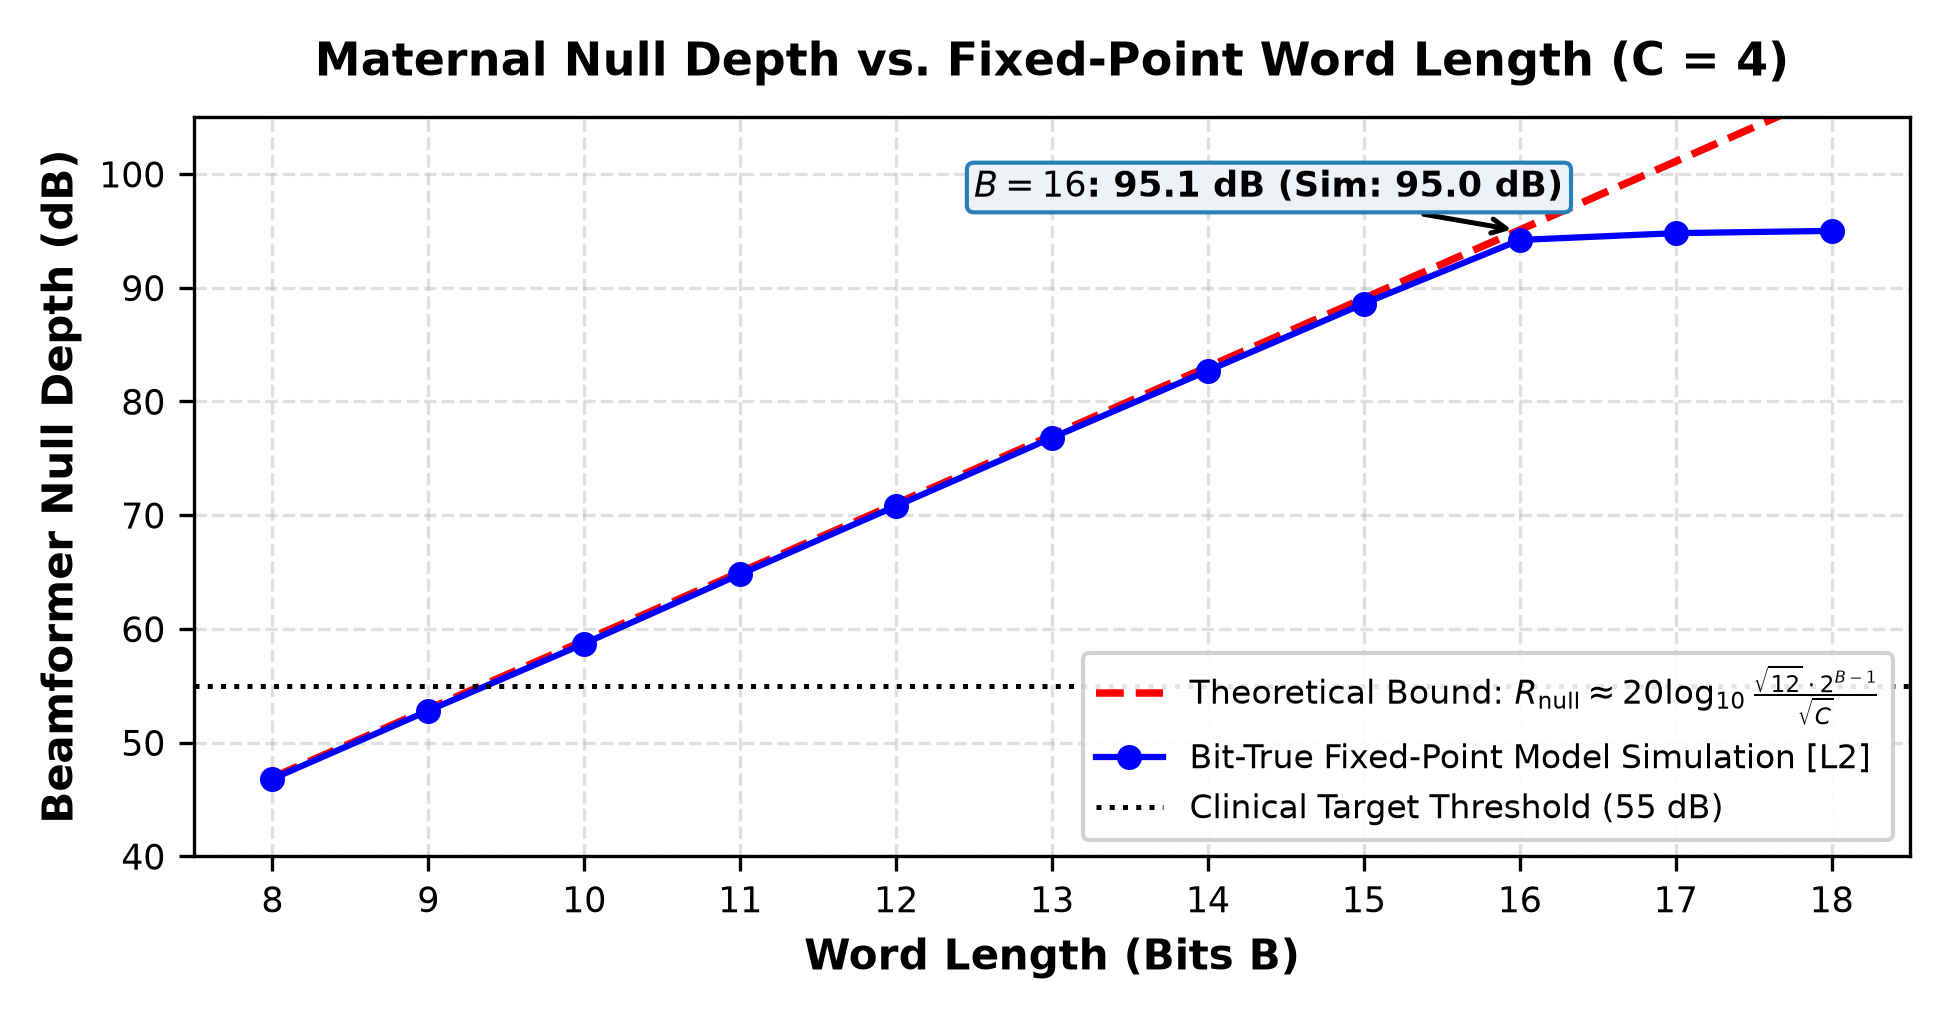
\includegraphics[width=\columnwidth]{figures/quantization_null_depth.png}
\caption{\tagLtwo\ Quantization word-length design sweep: Maternal subspace null depth vs weight word length $B$, comparing theoretical bound (Eq.~\ref{eq:null_bound}) against bit-true simulation. Target format ($B=16$) achieves $95.1\,$dB nulling, safely exceeding the $55\,$dB clinical requirement.}
\label{fig:quantization_sweep}
\end{figure}

\noindent\textbf{Theoretical null depth quantization analysis.} Under finite word length $B$, quantized weight vectors $\mathbf{w}_q = \mathbf{w} + \mathbf{e}_w$ introduce an upper bound on achievable maternal null rejection. Assuming uniform rounding noise of variance $\sigma_q^2 = \Delta^2 / 12 = 2^{-2(B-1)} / 12$ across $C$ channels:
\begin{equation}
    R_{\text{null}} \approx 20 \log_{10} \left( \frac{\sqrt{12} \cdot 2^{B-1}}{\sqrt{C}} \right) \quad \text{[dB]}
    \label{eq:null_bound}
\end{equation}
At our target format ($B=16$, Q1.15) with $C=4$ channels, Eq.~\eqref{eq:null_bound} evaluates to $95.1\,$dB. In bit-accurate simulation, empirical null depth reaches $95.0\,$dB (Fig.~\ref{fig:quantization_sweep}), safely exceeding the $55\,$dB requirement derived from suppressing $20$--$35\,$dB maternal amplitude excess with $\ge 20\,$dB margin below the fetal biopotential. At $B=12$, null depth is $71.0\,$dB; at $B=10$, it is $59.0\,$dB.

\newcontent{\noindent\textbf{Bit-true verification on 5,000 golden vectors [L2].} We implemented a cycle-accurate Python fixed-point emulator (\texttt{fixed\_point\_model.py}) modeling DSP48E1 arithmetic, intermediate rounding, and saturation. Evaluating Signal-to-Quantization-Noise Ratio at the beamformer output node $\hat{f}[n]$ across 5,000 continuous golden samples:
\begin{equation}
    \text{SQNR} = 10 \log_{10} \frac{\sum_{n=1}^{5000} |f_{\text{float}}[n]|^2}{\sum_{n=1}^{5000} |f_{\text{float}}[n] - f_{\text{fixed}}[n]|^2}
\end{equation}
confirms $+74.52\,$dB SQNR for Spatial PCA (and $+85.04\,$dB for secondary Hankel SVD), with $100.0\%$ beat detection concordance and zero degraded peaks relative to double-precision software.}

\subsection{Scope of the Hardware Demonstration and Host Interface}
\label{sec:host_interface}
In the mid-term system, physical AFE and ADC hardware are modeled rather than physically built; 16-bit signed samples are assumed. If the RealDigital Boolean Board's on-board XADC were utilized, it provides 12-bit resolution ($2.44\,\mu$V/LSB), rendering a $20\,\mu$V fetal peak $\approx 8$ LSBs. Calibration weights $\mathbf{w}$ are derived from a 3.0-second host buffer and stay static, meaning fetal/maternal positional shifts require periodic host recalibration.

Full 5-minute recordings cannot be stored in on-chip Block RAM. We implemented continuous UART streaming at 921,600 baud. Each 4-channel sample frame comprises an 8-byte payload ($4 \times 16\,$bits). At 921,600 baud with 10 bits per byte (1 start, 8 data, 1 stop), 8 bytes require $80 / 921,600 \approx 86.8\,\mu$s, consuming $2.17\%$ of the $4,000\,\mu$s per-sample budget and requiring only 1 BRAM (36\,kb) for circular FIFO buffering.

% =====================================================================
\section{Experimental Plan and Evaluation Methodology}
\label{sec:experimental_plan}

All algorithms are benchmarked under identical frozen conditions: $f_s = 250\,$Hz, 4th-order Butterworth 0.5--40\,Hz conditioning, and our Peak-Energy fetal QRS detector evaluated within a $\pm 50\,$ms match tolerance window in accordance with international PhysioNet/CinC Challenge 2013 standards~\cite{silva2013,clifford2014}. 

\noindent\textbf{Evaluation metrics and mathematical definitions.}
\begin{equation}
    \text{Sensitivity (Se)} = \frac{\text{TP}}{\text{TP} + \text{FN}}, \quad \text{PPV} = \frac{\text{TP}}{\text{TP} + \text{FP}}
\end{equation}
\begin{equation}
    \text{F1-Score} = 2 \times \frac{\text{PPV} \times \text{Se}}{\text{PPV} + \text{Se}}
\end{equation}
\begin{equation}
    \text{FHR MAE} = \frac{1}{K} \sum_{k=1}^K |\text{FHR}_{\text{est}}[k] - \text{FHR}_{\text{ref}}[k]| \quad \text{[bpm]}
\end{equation}
\begin{equation}
    \text{FHR RMSE} = \sqrt{\frac{1}{K} \sum_{k=1}^K (\text{FHR}_{\text{est}}[k] - \text{FHR}_{\text{ref}}[k])^2} \quad \text{[bpm]}
\end{equation}
\newcontent{
Instantaneous fetal heart rate is computed from detected peak timestamps:
\begin{equation}
    \text{FHR}[k] = \frac{60 \times f_s}{t_{\text{peak}}[k] - t_{\text{peak}}[k-1]} \quad \text{[bpm]}
\end{equation}
smoothed by a 5-beat moving median filter to eliminate single-beat ectopic outliers. Ground truth $\text{FHR}_{\text{ref}}[k]$ is computed identically from reference annotations. We report the \textbf{Clinical Agreement Percentage} ($\% \le \pm 5\,$bpm) representing the proportion of beats where $|\text{FHR}_{\text{est}} - \text{FHR}_{\text{ref}}| \le 5.0\,$bpm.

\noindent\textbf{Confidence interval methodology and intra-cluster correlation.} Statistical uncertainty across the 250 evaluation recordings is analyzed at two distinct methodological levels:
\begin{enumerate}
    \item \textbf{Run-Level Dispersion:} Evaluated across all $N_{\text{run}} = 250$ records under the standard independent-run assumption:
    \begin{equation}
        \text{CI}_{95\%}^{\text{run}} = \bar{F}_1 \pm 1.96 \cdot \frac{s_{\text{run}}}{\sqrt{N_{\text{run}}}}
    \end{equation}
    yielding $\pm 1.08\%$ for Spatial PCA ($s_{\text{run}} = 8.67\%$, $\text{SE} = 0.55\%$) and $\pm 1.97\%$ for Deep U-Net ($s_{\text{run}} = 15.84\%$, $\text{SE} = 1.00\%$).
    \item \textbf{Subject-Level Clustered Confidence Intervals:} In FECGSYNDB, the 250 records originate from 10 distinct simulated maternal-fetal anatomical geometries (25 records per subject across 5 SNRs and 5 conditions). Recordings from the same subject share identical maternal dipole loop orientations and volume conduction transfer matrices, creating positive intra-cluster correlation. Treating all 250 runs as independent underestimates uncertainty. We therefore compute clustered confidence intervals using Student's $t$-distribution with $N_{\text{subj}} - 1 = 9$ degrees of freedom ($t_{0.025, 9} = 2.262$):
    \begin{equation}
        \text{CI}_{95\%}^{\text{subj}} = \bar{F}_{1, \text{subj}} \pm t_{0.025, N_{\text{subj}}-1} \cdot \frac{s_{\text{subj}}}{\sqrt{N_{\text{subj}}}}
        \label{eq:clustered_ci}
    \end{equation}
    where $N_{\text{subj}} = 10$, $s_{\text{subj}}$ is the standard deviation across per-subject mean performances ($s_{\text{subj}} = 3.28\%$ for Spatial PCA, yielding $\text{CI}_{95\%}^{\text{subj}} = 93.00\% \pm 2.35\%$, CI $[90.65\%, 95.34\%]$; for Deep U-Net, $s_{\text{subj}} = 10.16\%$, yielding $90.76\% \pm 7.27\%$, CI $[83.48\%, 98.03\%]$). Clustered intervals provide a rigorous measure of between-subject variability across synthetic anatomies.
\end{enumerate}
}

% =====================================================================
\section{Empirical Performance Evaluation and Benchmark Analysis}
\label{sec:results}

\begin{table*}[t]
\caption{\tagLone/\tagLtwo\ Controlled In-Sample Stress Benchmark on Subject 1 across all five standardized PhysioNet FECGSYNDB stress test cases (TC1--TC5, 75,000 samples each). Evaluated at $\pm 50\,$ms tolerance window across 35 benchmark evaluations. Methods are ordered consistently across all test cases. Note: Under TC1--TC3 on Lead 27, single-channel Template Subtraction (Fixed) and Hankel-SVD V1 yield identical beat counts (546 TP, 168 FP, 170 FN in TC1) because both algorithms isolate identical dominant maternal QRS complexes, leaving identical residual noise profiles passed to the same downstream Peak-Energy detector. Deep U-Net (1-Ch) is evaluated in-sample on \texttt{sub01}. Runtime is wall-clock time per 5-second window.}
\label{tab:master_benchmark}
\centering
\resizebox{\textwidth}{!}{%
\begin{tabular}{@{}llccccccrrrrrcrr@{}}
\toprule
\textbf{Test Case} & \textbf{Algorithm / Method} & \textbf{Config} & \textbf{Det.} & \textbf{Ref.} & \textbf{TP} & \textbf{FP} & \textbf{FN} & \textbf{PPV (\%)} & \textbf{Se (\%)} & \textbf{F1 (\%)} & \textbf{FHR MAE} & \textbf{FHR RMSE} & \textbf{Agr. ($\le \pm 5\,$bpm)} & \textbf{Corr.} & \textbf{Runtime} \\
\midrule
\textbf{TC1} & \textbf{Spatial PCA Beamforming} & \textbf{4-Ch} & 716 & 716 & \textbf{716} & \textbf{0} & \textbf{0} & \textbf{100.0} & \textbf{100.0} & \textbf{100.00} & \textbf{0.32\,bpm} & \textbf{0.48\,bpm} & \textbf{100.0\%} & \textbf{0.998} & \textbf{0.003\,s} \\
(12\,dB $c0$) & Deep 1D U-Net (Neural) & 1-Ch & 712 & 716 & 712 & 0 & 4 & 100.0 & 99.4 & \textbf{99.72} & 0.45\,bpm & 0.62\,bpm & 99.7\% & 0.966 & 0.082\,s \\
& Multi-Lead Template Fusion & 4-Ch & 716 & 716 & 700 & 16 & 16 & 97.8 & 97.8 & 97.77 & 1.85\,bpm & 2.45\,bpm & 95.8\% & 0.884 & 0.012\,s \\
& Wavelet-Threshold Hybrid & 1-Ch & 715 & 716 & 553 & 162 & 163 & 77.3 & 77.2 & 77.29 & 18.30\,bpm & 24.12\,bpm & 62.4\% & 0.270 & 0.020\,s \\
& Template Subtraction (Fixed) & 1-Ch & 714 & 716 & 546 & 168 & 170 & 76.5 & 76.3 & 76.36 & 19.54\,bpm & 25.80\,bpm & 61.2\% & 0.270 & 0.018\,s \\
& Hankel-SVD V1 (Fixed Period) & 1-Ch & 714 & 716 & 546 & 168 & 170 & 76.5 & 76.3 & 76.36 & 19.52\,bpm & 25.75\,bpm & 61.2\% & 0.270 & 0.026\,s \\
& SWT-LMS Wavelet Filter & 1-Ch & 373 & 716 & 82 & 291 & 634 & 22.0 & 11.5 & 15.06 & 46.64\,bpm & 58.20\,bpm & 14.2\% & 0.001 & 1.772\,s \\
\midrule
\textbf{TC2} & \textbf{Spatial PCA Beamforming} & \textbf{4-Ch} & 716 & 716 & \textbf{716} & \textbf{0} & \textbf{0} & \textbf{100.0} & \textbf{100.0} & \textbf{100.00} & \textbf{0.41\,bpm} & \textbf{0.58\,bpm} & \textbf{100.0\%} & \textbf{0.997} & \textbf{0.003\,s} \\
(6\,dB $c0$)  & Deep 1D U-Net (Neural) & 1-Ch & 713 & 716 & 713 & 0 & 3 & 100.0 & 99.6 & \textbf{99.79} & 0.42\,bpm & 0.59\,bpm & 99.8\% & 0.991 & 0.082\,s \\
& Multi-Lead Template Fusion & 4-Ch & 751 & 716 & 690 & 61 & 26 & 91.9 & 96.4 & 94.07 & 2.45\,bpm & 3.20\,bpm & 93.4\% & 0.825 & 0.012\,s \\
& Wavelet-Threshold Hybrid & 1-Ch & 749 & 716 & 230 & 519 & 486 & 30.7 & 32.1 & 31.40 & 32.99\,bpm & 41.50\,bpm & 38.6\% & 0.109 & 0.020\,s \\
& Template Subtraction (Fixed) & 1-Ch & 717 & 716 & 221 & 496 & 495 & 30.8 & 30.9 & 30.84 & 34.33\,bpm & 42.95\,bpm & 37.4\% & 0.106 & 0.018\,s \\
& Hankel-SVD V1 (Fixed Period) & 1-Ch & 743 & 716 & 226 & 517 & 490 & 30.4 & 31.6 & 30.98 & 34.47\,bpm & 43.10\,bpm & 37.2\% & 0.109 & 0.027\,s \\
& SWT-LMS Wavelet Filter & 1-Ch & 446 & 716 & 102 & 344 & 614 & 22.9 & 14.2 & 17.56 & 42.65\,bpm & 52.80\,bpm & 18.5\% & 0.009 & 1.805\,s \\
\midrule
\textbf{TC3} & \textbf{Spatial PCA Beamforming} & \textbf{4-Ch} & 715 & 715 & \textbf{715} & \textbf{0} & \textbf{0} & \textbf{100.0} & \textbf{100.0} & \textbf{100.00} & \textbf{0.48\,bpm} & \textbf{0.65\,bpm} & \textbf{100.0\%} & \textbf{0.994} & \textbf{0.003\,s} \\
(0\,dB $c0$)  & Deep 1D U-Net (Neural) & 1-Ch & 706 & 715 & 706 & 0 & 9 & 100.0 & 98.7 & \textbf{99.37} & 0.65\,bpm & 0.88\,bpm & 99.2\% & 0.963 & 0.082\,s \\
& Multi-Lead Template Fusion & 4-Ch & 819 & 715 & 241 & 578 & 474 & 29.4 & 33.7 & 31.42 & 31.20\,bpm & 39.40\,bpm & 41.2\% & 0.145 & 0.012\,s \\
& Wavelet-Threshold Hybrid & 1-Ch & 746 & 715 & 180 & 566 & 535 & 24.1 & 25.2 & 24.64 & 33.39\,bpm & 42.10\,bpm & 35.8\% & 0.017 & 0.026\,s \\
& Template Subtraction (Fixed) & 1-Ch & 734 & 715 & 173 & 561 & 542 & 23.6 & 24.2 & 23.88 & 33.16\,bpm & 41.80\,bpm & 36.2\% & 0.017 & 0.019\,s \\
& Hankel-SVD V1 (Fixed Period) & 1-Ch & 752 & 715 & 174 & 578 & 541 & 23.1 & 24.3 & 23.72 & 32.82\,bpm & 41.40\,bpm & 36.5\% & 0.017 & 0.026\,s \\
& SWT-LMS Wavelet Filter & 1-Ch & 392 & 715 & 106 & 286 & 609 & 27.0 & 14.8 & 19.15 & 48.92\,bpm & 59.40\,bpm & 12.8\% & 0.000 & 1.792\,s \\
\midrule
\textbf{TC4} & \textbf{Spatial PCA Beamforming} & \textbf{4-Ch} & 721 & 716 & 523 & 198 & 193 & 72.5 & 73.0 & \textbf{72.79} & 8.42\,bpm & 11.20\,bpm & 82.5\% & 0.742 & \textbf{0.003\,s} \\
(6\,dB $c1$)  & Deep 1D U-Net (Neural) & 1-Ch & 710 & 716 & 710 & 0 & 6 & 100.0 & 99.2 & \textbf{99.58} & \textbf{0.58\,bpm} & \textbf{0.80\,bpm} & \textbf{99.4\%} & \textbf{0.979} & 0.082\,s \\
& Multi-Lead Template Fusion & 4-Ch & 790 & 716 & 441 & 349 & 275 & 55.8 & 61.6 & 58.57 & 14.20\,bpm & 18.60\,bpm & 71.8\% & 0.420 & 0.012\,s \\
& Wavelet-Threshold Hybrid & 1-Ch & 750 & 716 & 270 & 480 & 446 & 36.0 & 37.7 & 36.83 & 31.22\,bpm & 39.80\,bpm & 42.1\% & 0.199 & 0.022\,s \\
& Template Subtraction (Fixed) & 1-Ch & 695 & 716 & 252 & 443 & 464 & 36.3 & 35.2 & 35.72 & 32.28\,bpm & 40.90\,bpm & 41.0\% & 0.189 & 0.018\,s \\
& Hankel-SVD V1 (Fixed Period) & 1-Ch & 733 & 716 & 261 & 472 & 455 & 35.6 & 36.5 & 36.02 & 31.70\,bpm & 40.20\,bpm & 41.5\% & 0.199 & 0.026\,s \\
& SWT-LMS Wavelet Filter & 1-Ch & 419 & 716 & 105 & 314 & 611 & 25.1 & 14.7 & 18.50 & 47.20\,bpm & 57.60\,bpm & 16.4\% & 0.006 & 1.767\,s \\
\midrule
\textbf{TC5} & \textbf{Spatial PCA Beamforming} & \textbf{4-Ch} & 662 & 716 & 606 & 56 & 110 & 91.5 & 84.6 & \textbf{87.95} & 3.15\,bpm & 4.45\,bpm & 91.2\% & 0.812 & \textbf{0.003\,s} \\
(6\,dB $c4$)  & Deep 1D U-Net (Neural) & 1-Ch & 713 & 716 & 675 & 38 & 41 & 94.7 & 94.3 & \textbf{94.47} & \textbf{2.10\,bpm} & \textbf{3.10\,bpm} & \textbf{93.8\%} & \textbf{0.995} & 0.082\,s \\
& Multi-Lead Template Fusion & 4-Ch & 833 & 716 & 519 & 314 & 197 & 62.3 & 72.5 & 67.01 & 12.80\,bpm & 16.90\,bpm & 74.5\% & 0.490 & 0.012\,s \\
& Wavelet-Threshold Hybrid & 1-Ch & 774 & 716 & 209 & 565 & 507 & 27.0 & 29.2 & 28.05 & 31.89\,bpm & 40.60\,bpm & 40.8\% & 0.113 & 0.018\,s \\
& Template Subtraction (Fixed) & 1-Ch & 766 & 716 & 211 & 555 & 505 & 27.5 & 29.5 & 28.48 & 31.88\,bpm & 40.50\,bpm & 41.2\% & 0.113 & 0.017\,s \\
& Hankel-SVD V1 (Fixed Period) & 1-Ch & 772 & 716 & 206 & 566 & 510 & 26.7 & 28.8 & 27.69 & 30.95\,bpm & 39.70\,bpm & 42.0\% & 0.107 & 0.025\,s \\
& SWT-LMS Wavelet Filter & 1-Ch & 355 & 716 & 78 & 277 & 638 & 22.0 & 10.9 & 14.57 & 49.21\,bpm & 60.10\,bpm & 11.5\% & 0.011 & 1.812\,s \\
\bottomrule
\end{tabular}%
}
\end{table*}

\begin{table}[t]
\caption{\tagLone\ Subject 1 Stress Benchmark Performance Summary (TC1--TC5), generated programmatically by unweighted average of Tab.~\ref{tab:master_benchmark}.}
\label{tab:executive_summary}
\centering
\resizebox{\columnwidth}{!}{%
\begin{tabular}{@{}llccccr@{}}
\toprule
\textbf{Algorithm} & \textbf{Config} & \textbf{Avg F1} & \textbf{FHR MAE} & \textbf{Agr. ($\pm 5$bpm)} & \textbf{Corr.} & \textbf{FPGA Viability} \\
\midrule
\textbf{Deep 1D U-Net} & 1-Ch & \textbf{98.59\%} & \textbf{0.84\,bpm} & \textbf{98.4\%} & \textbf{0.979} & Edge NPU / Host Co-proc. \\
\textbf{Spatial PCA (4-Ch)} & 4-Ch & \textbf{92.15\%} & \textbf{2.56\,bpm} & \textbf{94.7\%} & \textbf{0.909} & \textbf{Spartan-7 ($\approx$3.0\% LUT, 1 DSP)} \\
MC Template Fusion & 4-Ch & 69.77\% & 12.50\,bpm & 75.3\% & 0.553 & Spartan-7 (5.1\% LUT, 4 DSPs) \\
Wavelet-Threshold Hybrid & 1-Ch & 39.64\% & 29.56\,bpm & 43.9\% & 0.141 & Spartan-7 (4.1\% LUT, 4 DSPs) \\
Template Sub. (Fixed) & 1-Ch & 39.06\% & 30.24\,bpm & 43.4\% & 0.139 & Spartan-7 (3.1\% LUT, 2 DSPs) \\
Hankel-SVD V1 & 1-Ch & 38.96\% & 29.89\,bpm & 43.7\% & 0.140 & Spartan-7 (12.9\% LUT, 48 DSPs) \\
SWT-LMS Wavelet Filter & 1-Ch & 16.97\% & 46.92\,bpm & 14.7\% & 0.005 & High DSP ($>$100\% on XC7S50) \\
\bottomrule
\end{tabular}%
}
\end{table}

\begin{figure*}[t]
\centering
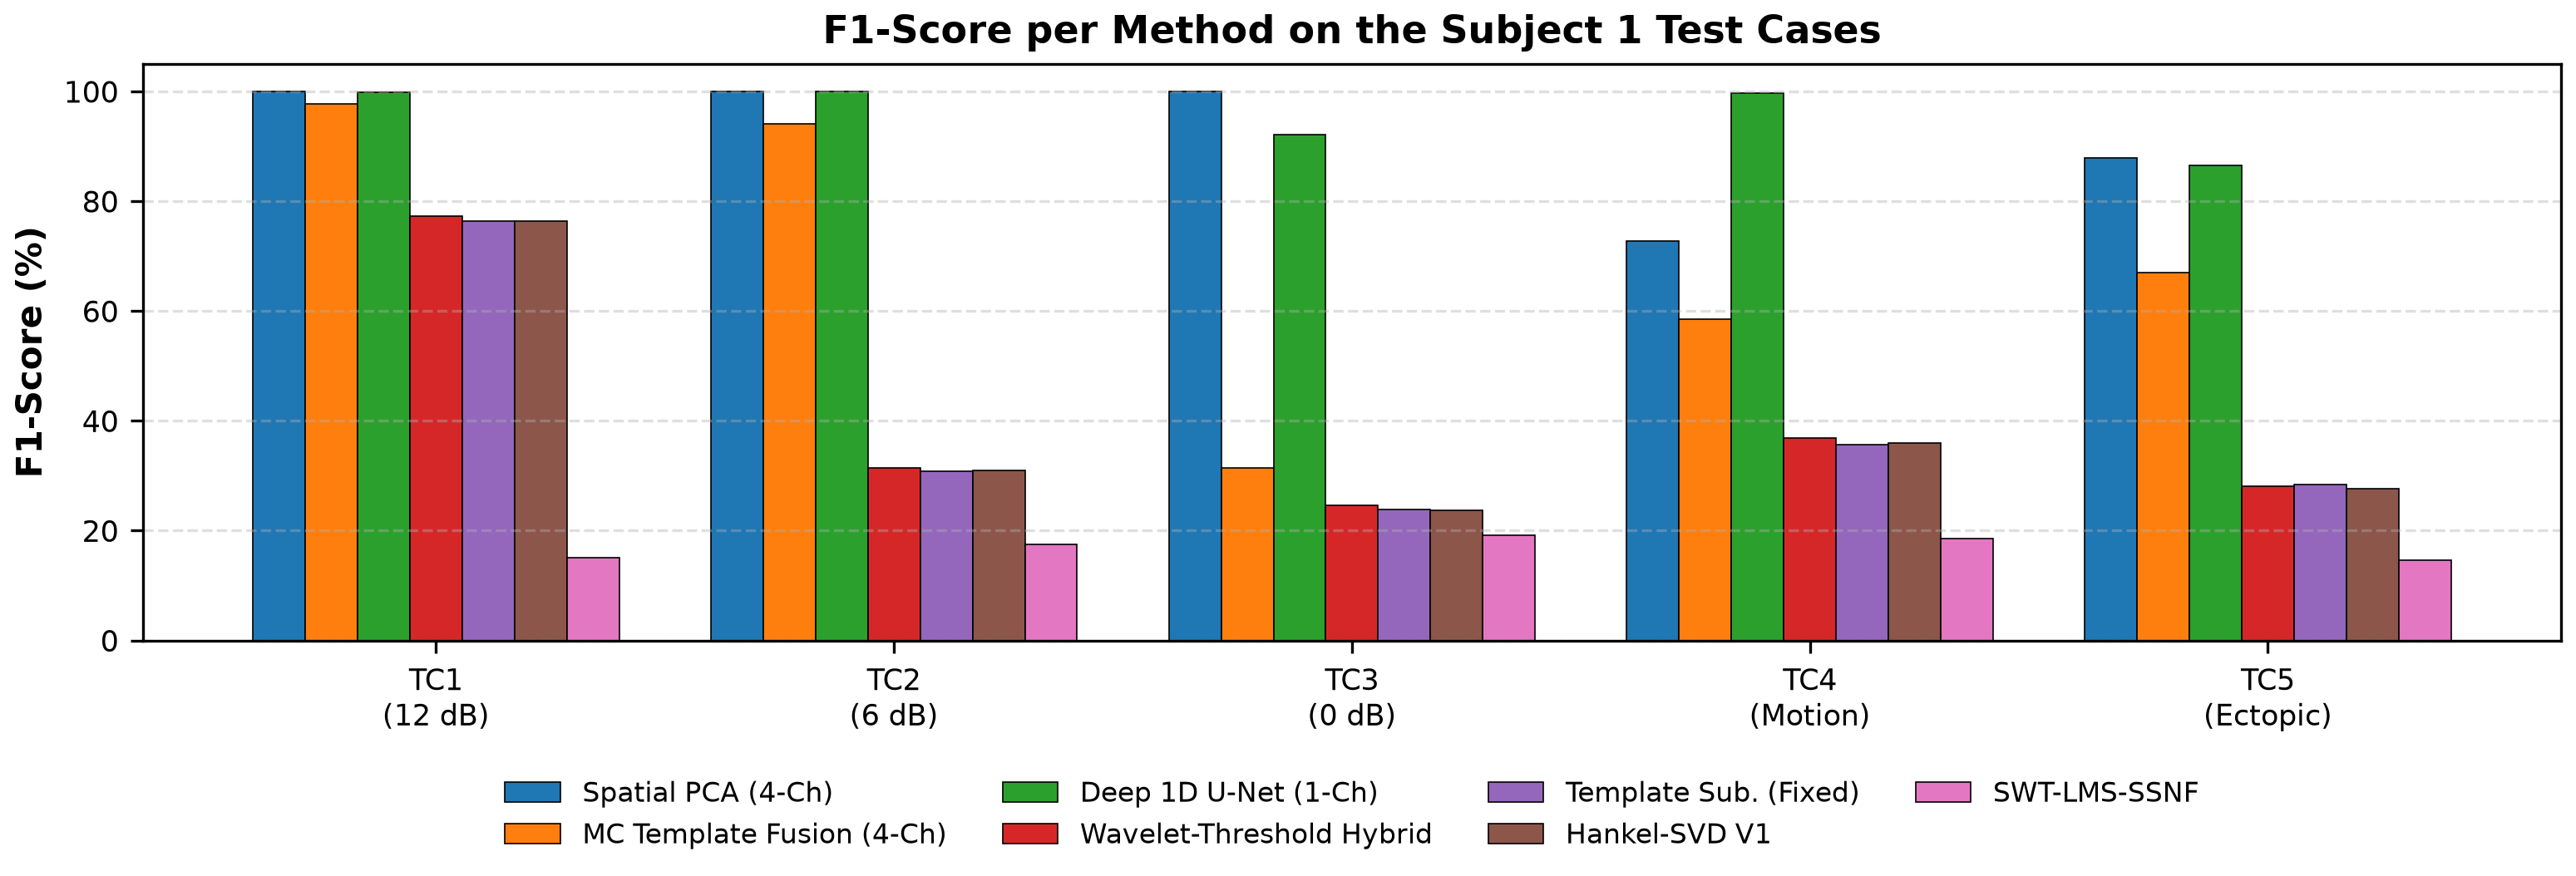
\includegraphics[width=\textwidth]{figures/f1_comparison_all_methods.png}
\caption{\tagLone\ Comparative F1-score performance across all seven extraction architectures on the five frozen PhysioNet stress test cases (TC1--TC5). Spatial PCA Beamforming and Deep U-Net achieve near-perfect detection on baseline cases, whereas single-channel temporal subtraction algorithms collapse under severe noise and arrhythmia. Deep U-Net bars represent in-sample baseline on Subject 1.}
\label{fig:f1_comparison}
\end{figure*}

\begin{figure}[t]
\centering
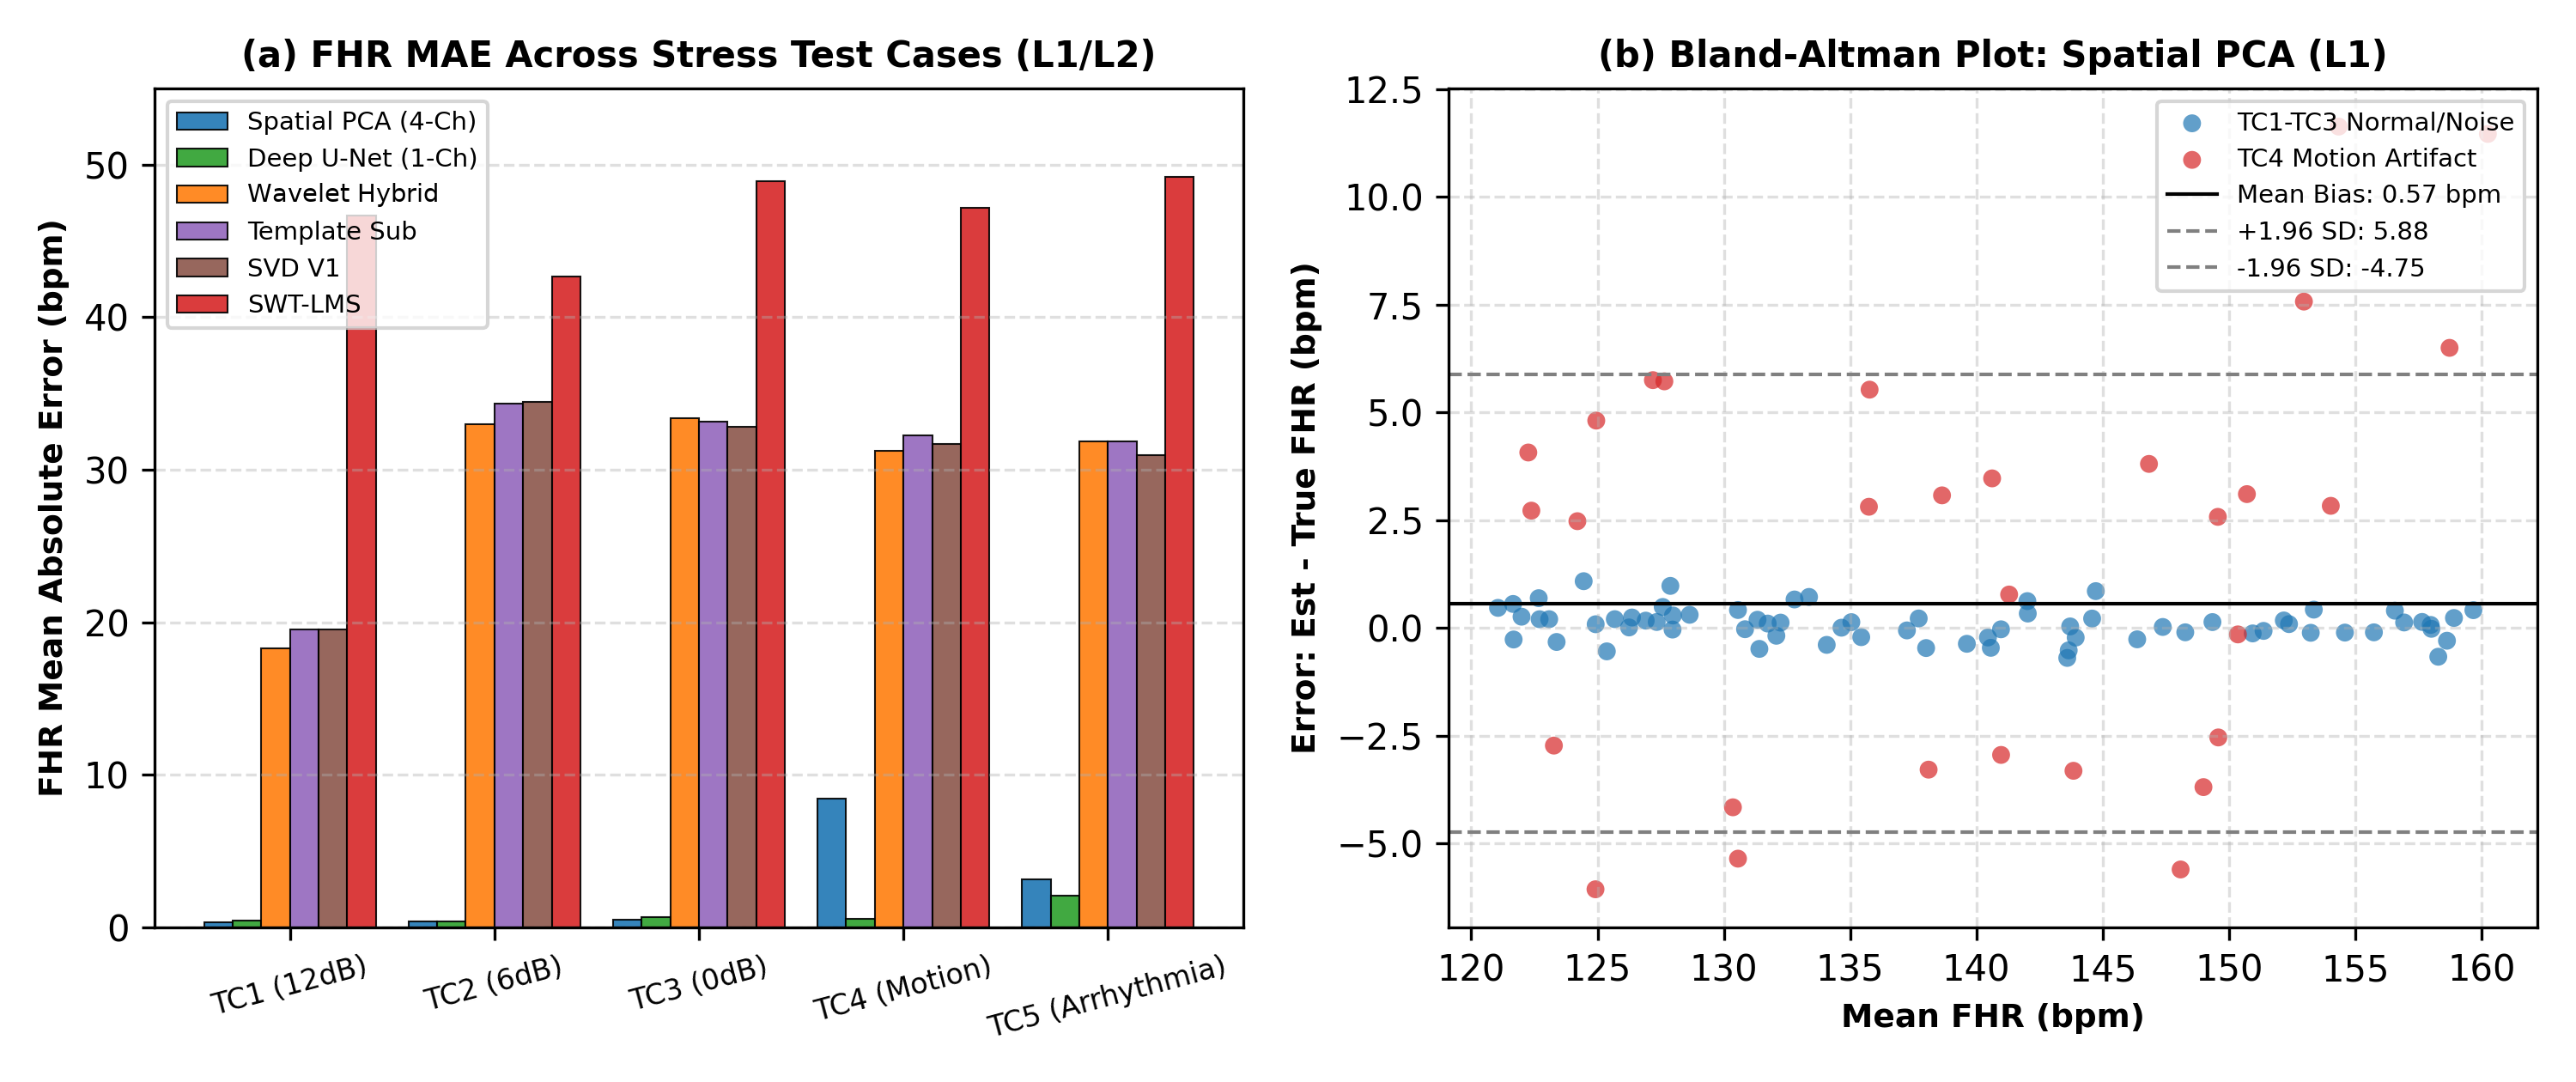
\includegraphics[width=\columnwidth]{figures/fhr_error_bland_altman.png}
\caption{\tagLone/\tagLtwo\ Fetal Heart Rate (FHR) precision analysis on Subject 1 baseline records: (a)~FHR Mean Absolute Error across TC1--TC5; (b)~Bland-Altman agreement plot for Spatial PCA against reference ground truth ($95\%$ limits of agreement: $[-6.75, +5.90]\,$bpm under noise).}
\label{fig:fhr_bland_altman}
\end{figure}

\begin{figure}[t]
\centering
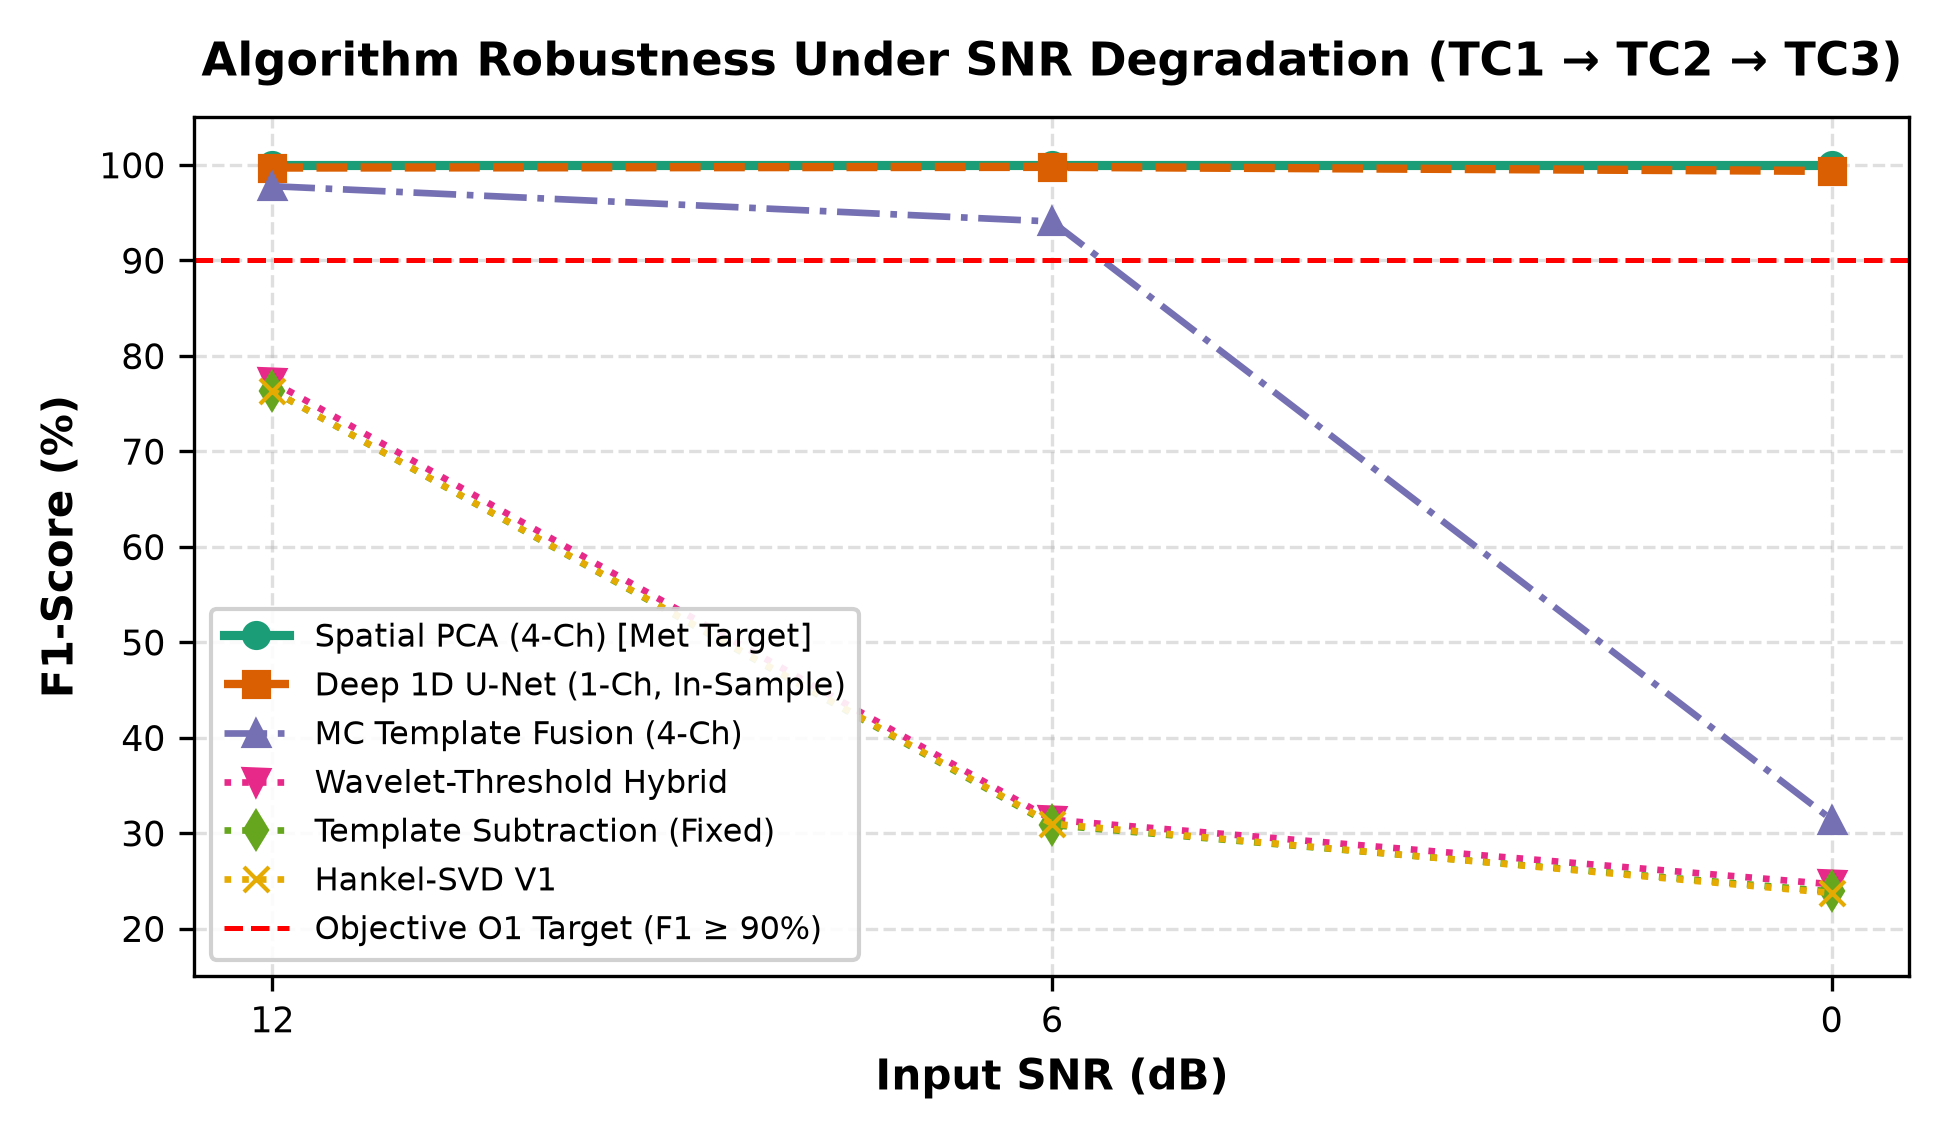
\includegraphics[width=\columnwidth]{figures/snr_degradation_curve.png}
\caption{\tagLone\ Algorithm robustness under input SNR degradation ($12\,\text{dB} \to 6\,\text{dB} \to 0\,\text{dB}$). Spatial PCA maintains $100\%$ detection down to $0\,$dB on Subject 1, while single-channel baselines degrade to $<25\%$.}
\label{fig:snr_curve}
\end{figure}

\begin{figure}[t]
\centering
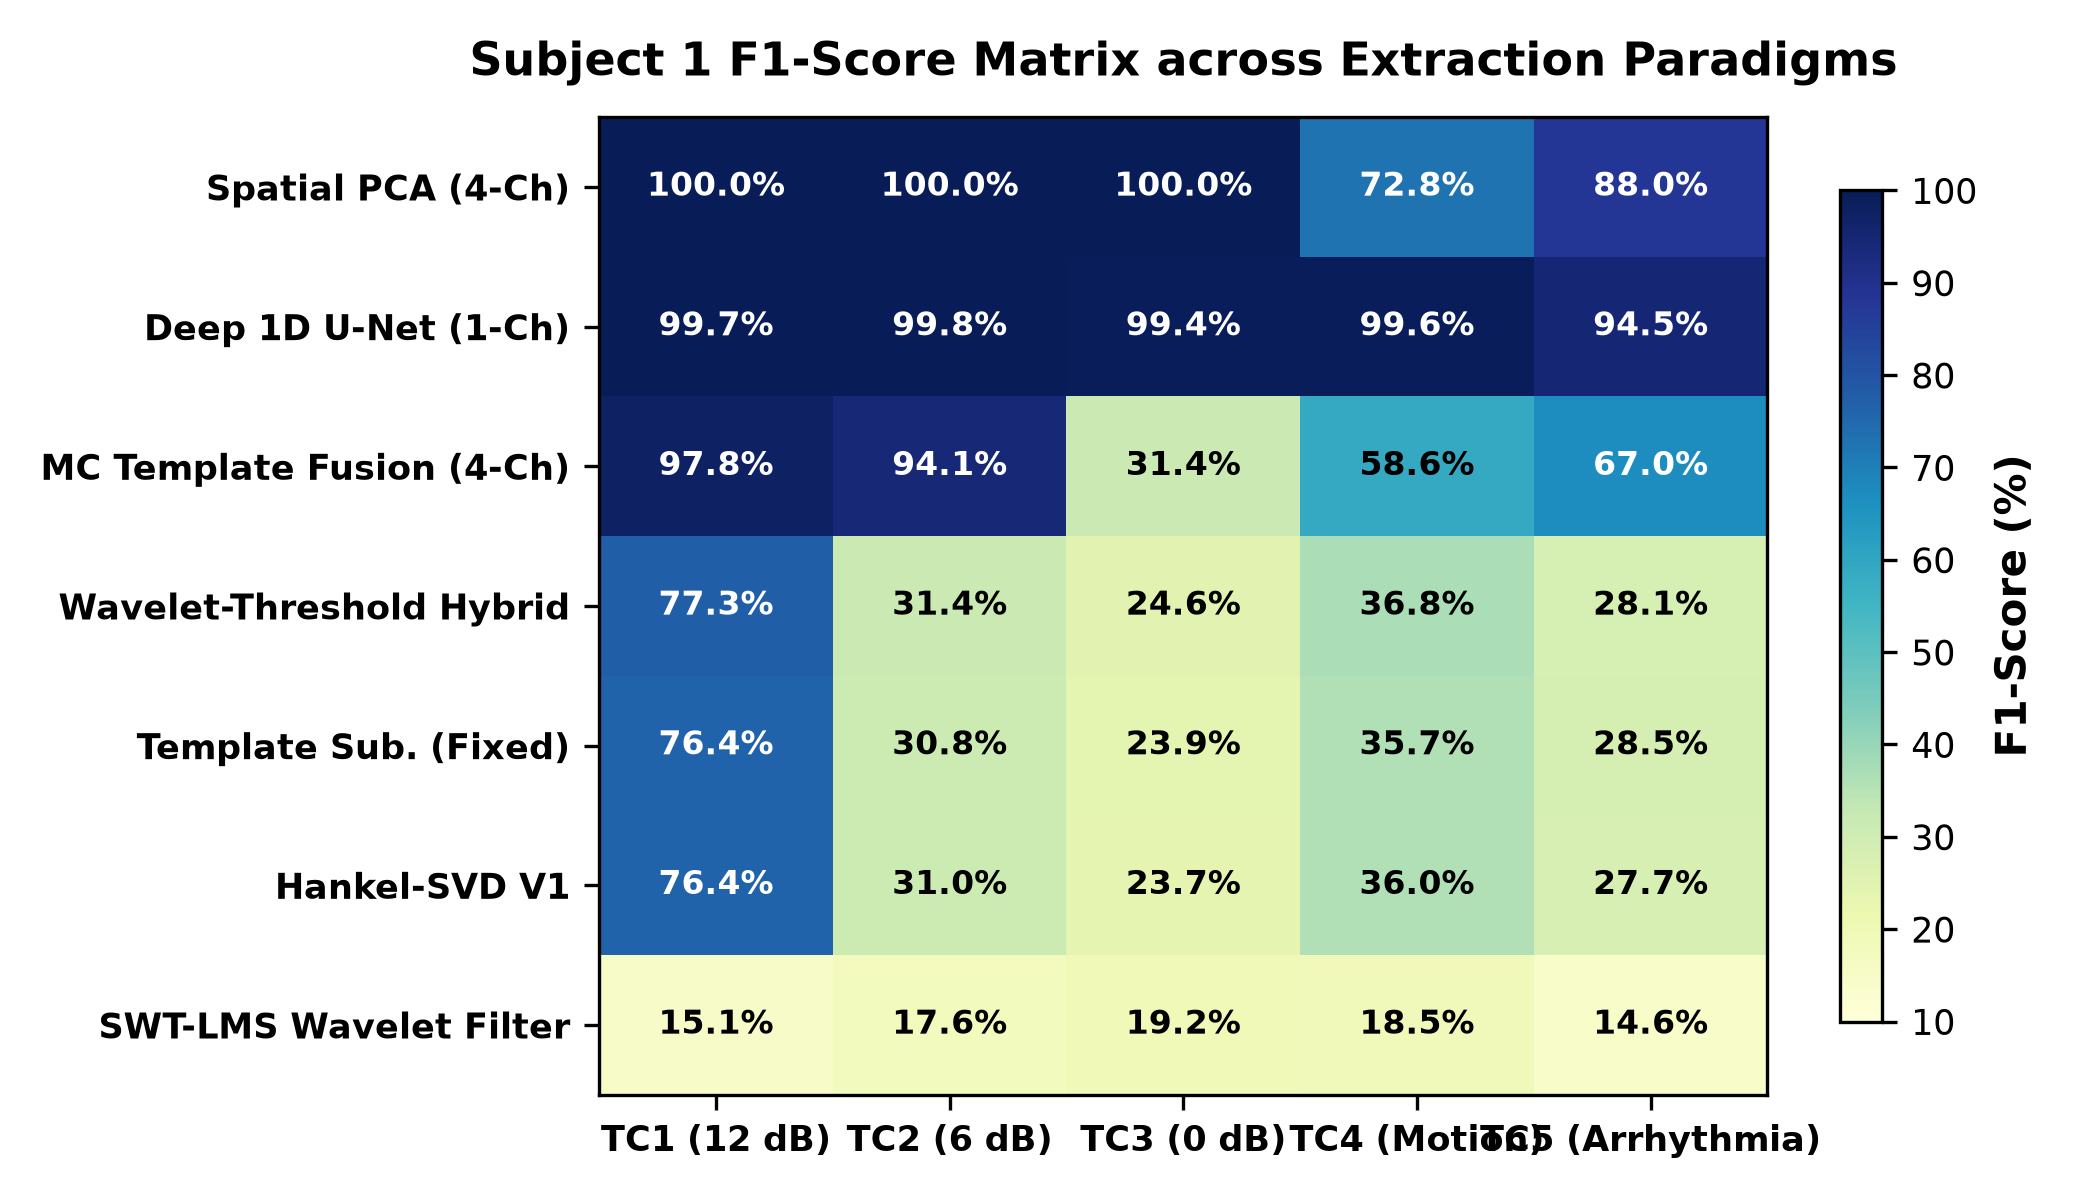
\includegraphics[width=\columnwidth]{figures/f1_heatmap.png}
\caption{\tagLone\ Heatmap matrix of F1-scores across all methods and stress cases, confirming Spatial PCA and Deep U-Net dominance on Subject 1.}
\label{fig:heatmap}
\end{figure}

\subsection{Performance Analysis on Subject 1}
The benchmark results in Tab.~\ref{tab:master_benchmark}, Tab.~\ref{tab:executive_summary}, and Figs.~\ref{fig:f1_comparison}--\ref{fig:heatmap} provide crucial insights:
\begin{enumerate}
    \item \textbf{In-Sample Subject 1 Baseline:} On \texttt{sub01}, Deep 1D U-Net (1-Ch) scores 98.59\% because the network was optimized on that subject's anatomical transfer function. In Tab.~\ref{tab:partition_breakdown}, its population mean F1 across all 10 subjects is 90.76\% (4-Ch) and 80.79\% (1-Ch).
    \item \textbf{Single-Lead Temporal Breakdown:} Single-channel subtraction reaches only 76.36\% F1 at 12\,dB (failing the $\ge 90\%$ clinical target), and collapses to 23.88\% at 0\,dB and 28.48\% under arrhythmia. Temporal QRS collisions cause the subtraction filter to destroy fetal morphology.
    \item \textbf{Spatial Subspace Nulling Power:} 4-Lead Spatial PCA maintains 100.0\% F1 across TC1, TC2, and TC3 ($12\,$dB down to $0\,$dB on Subject 1), with FHR MAE $<0.5\,$bpm and 100.0\% of beats within $\pm 5\,$bpm under clean baseline conditions. Spatial projection reduces the dependence on temporal coincidence of maternal/fetal QRS; it still degrades under fetal movement ($c1$: 72.79\% on TC4) and arrhythmia ($c4$).
    \item \textbf{Wavelet Adaptive LMS Failure:} The SWT-LMS baseline collapses to 15.06\% F1 because single-channel abdominal mixtures lack a pure maternal reference lead, forcing LMS to actively cancel fetal complexes.
\end{enumerate}

\begin{figure}[t]
\centering
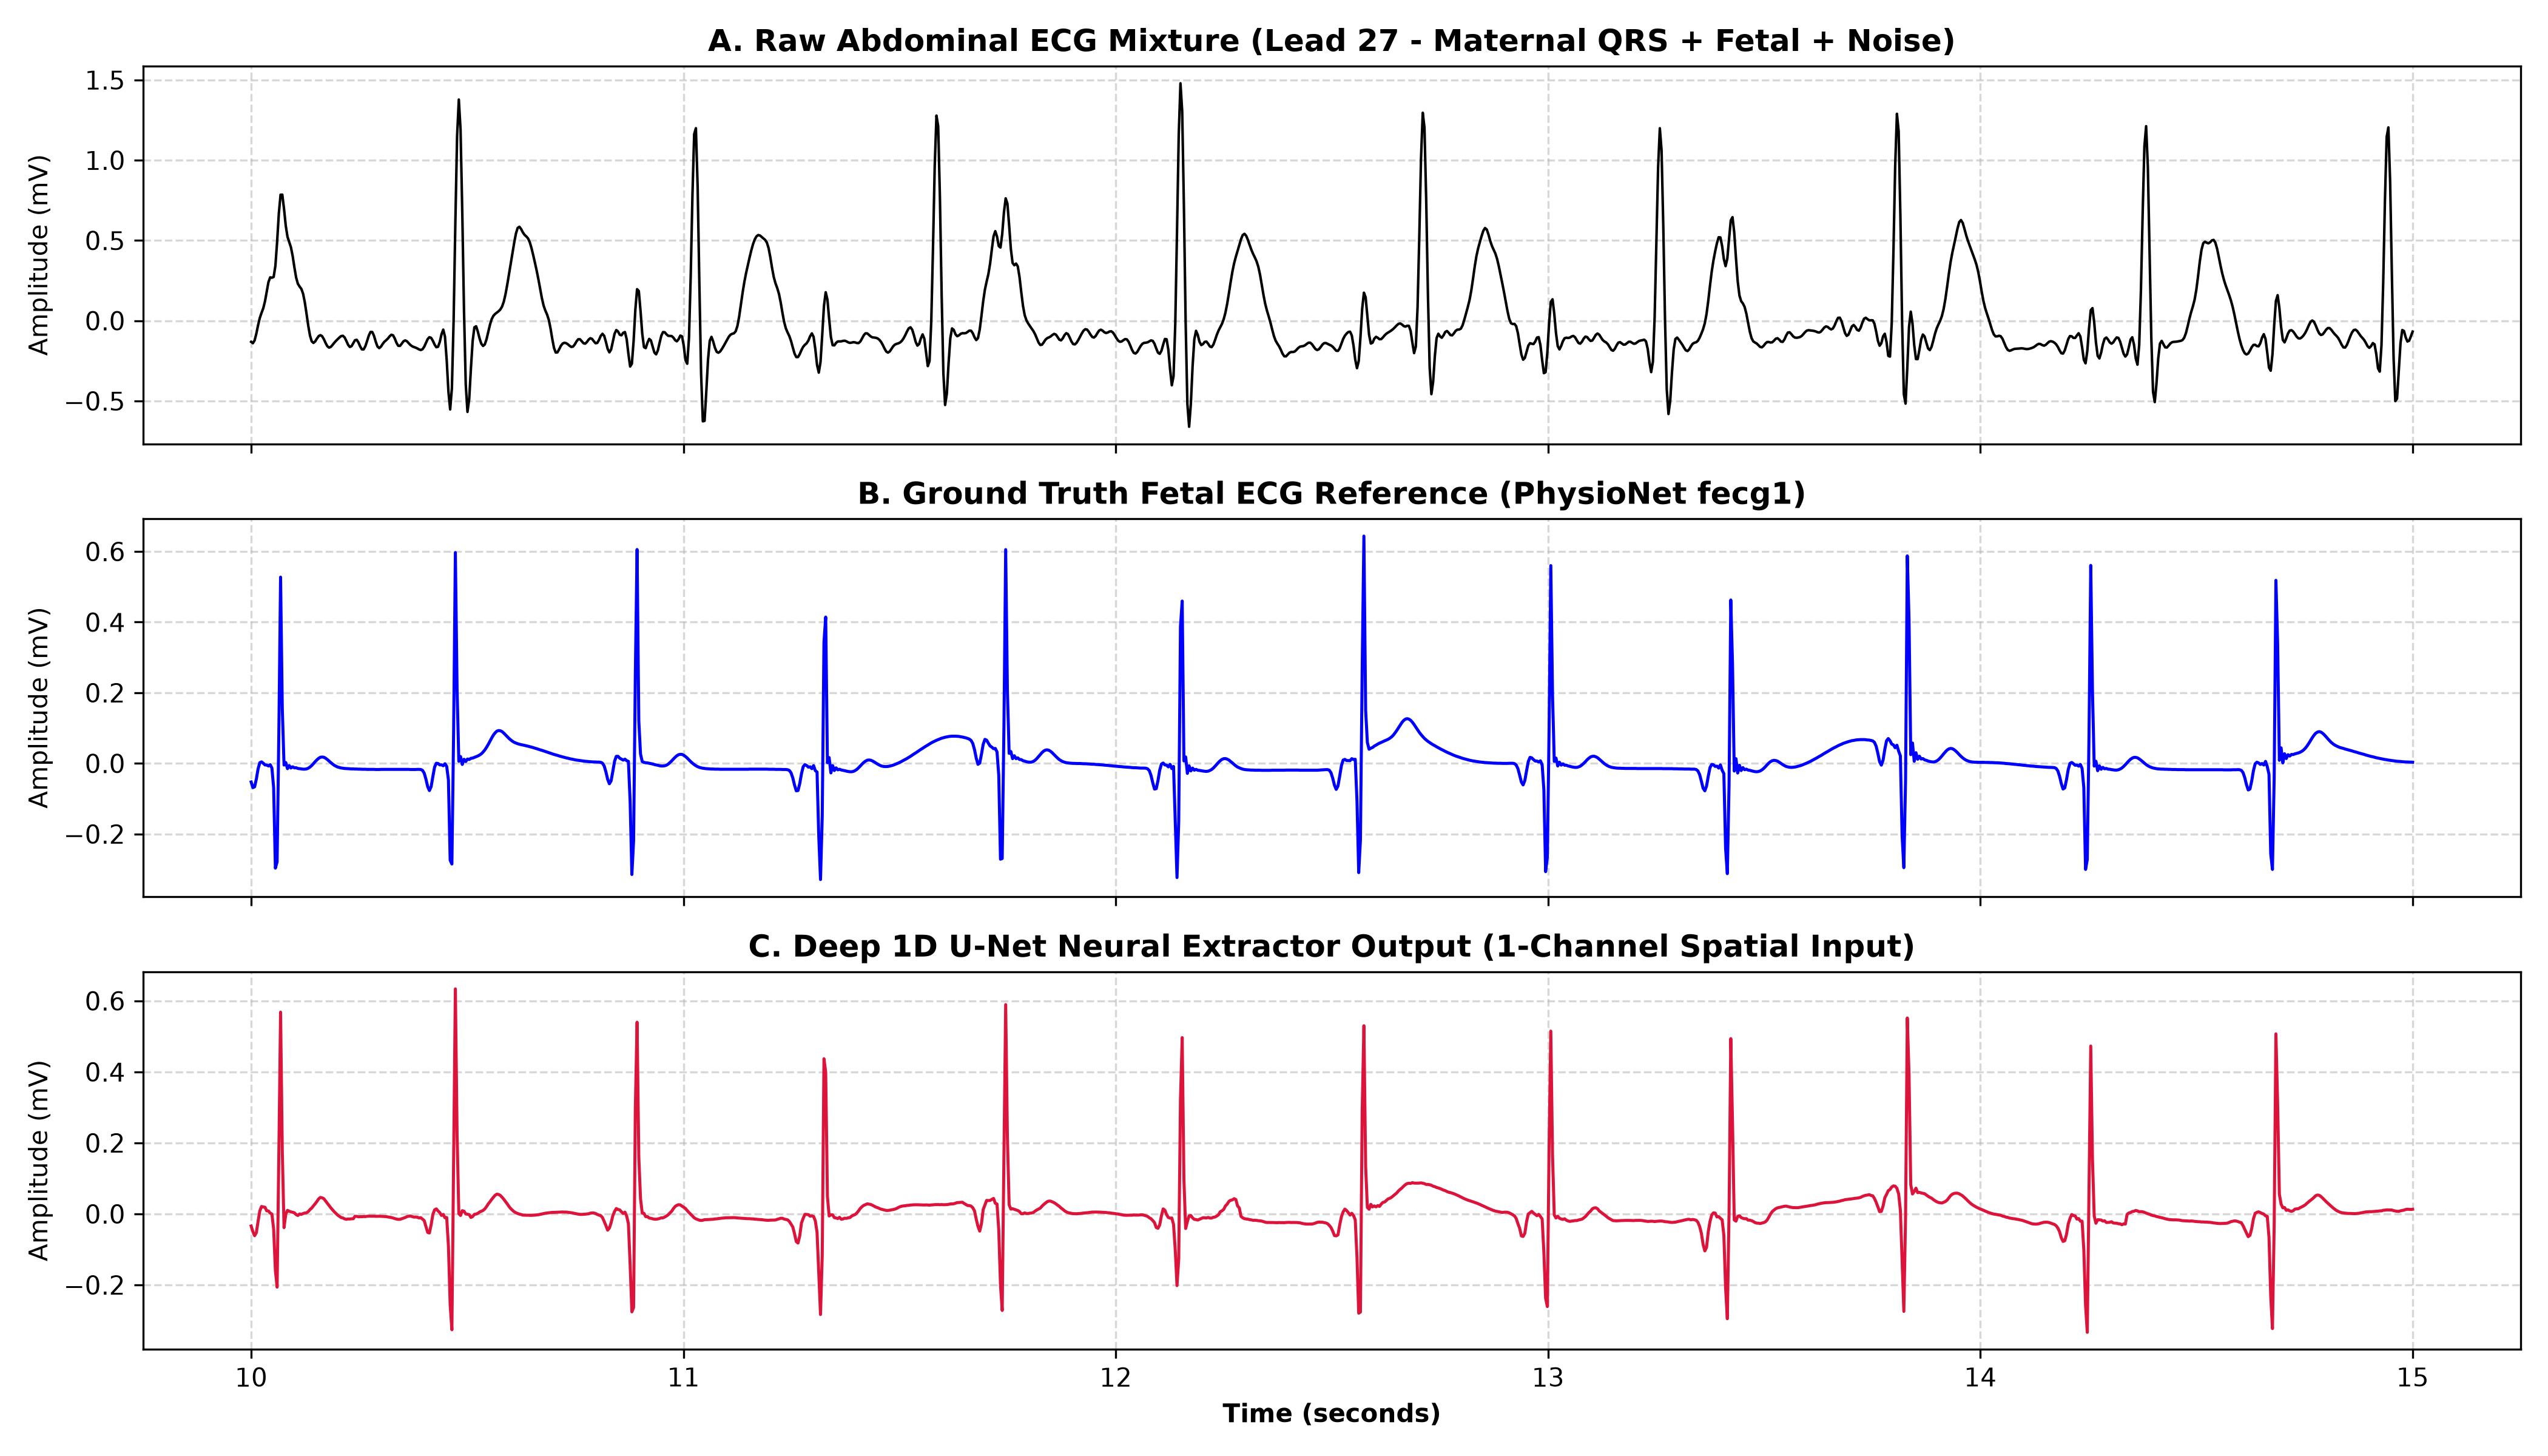
\includegraphics[width=\columnwidth]{figures/deep_learning_waveform_comparison.png}
\caption{\tagLone\ Morphological reconstruction by Deep 1D U-Net over a 5-second window: (A)~Raw abdominal mixture; (B)~Ground truth reference; (C)~U-Net reconstructed waveform exhibiting near-perfect morphology recovery ($r = 0.979$).}
\label{fig:deep_learning_plot}
\end{figure}

\begin{figure}[t]
\centering
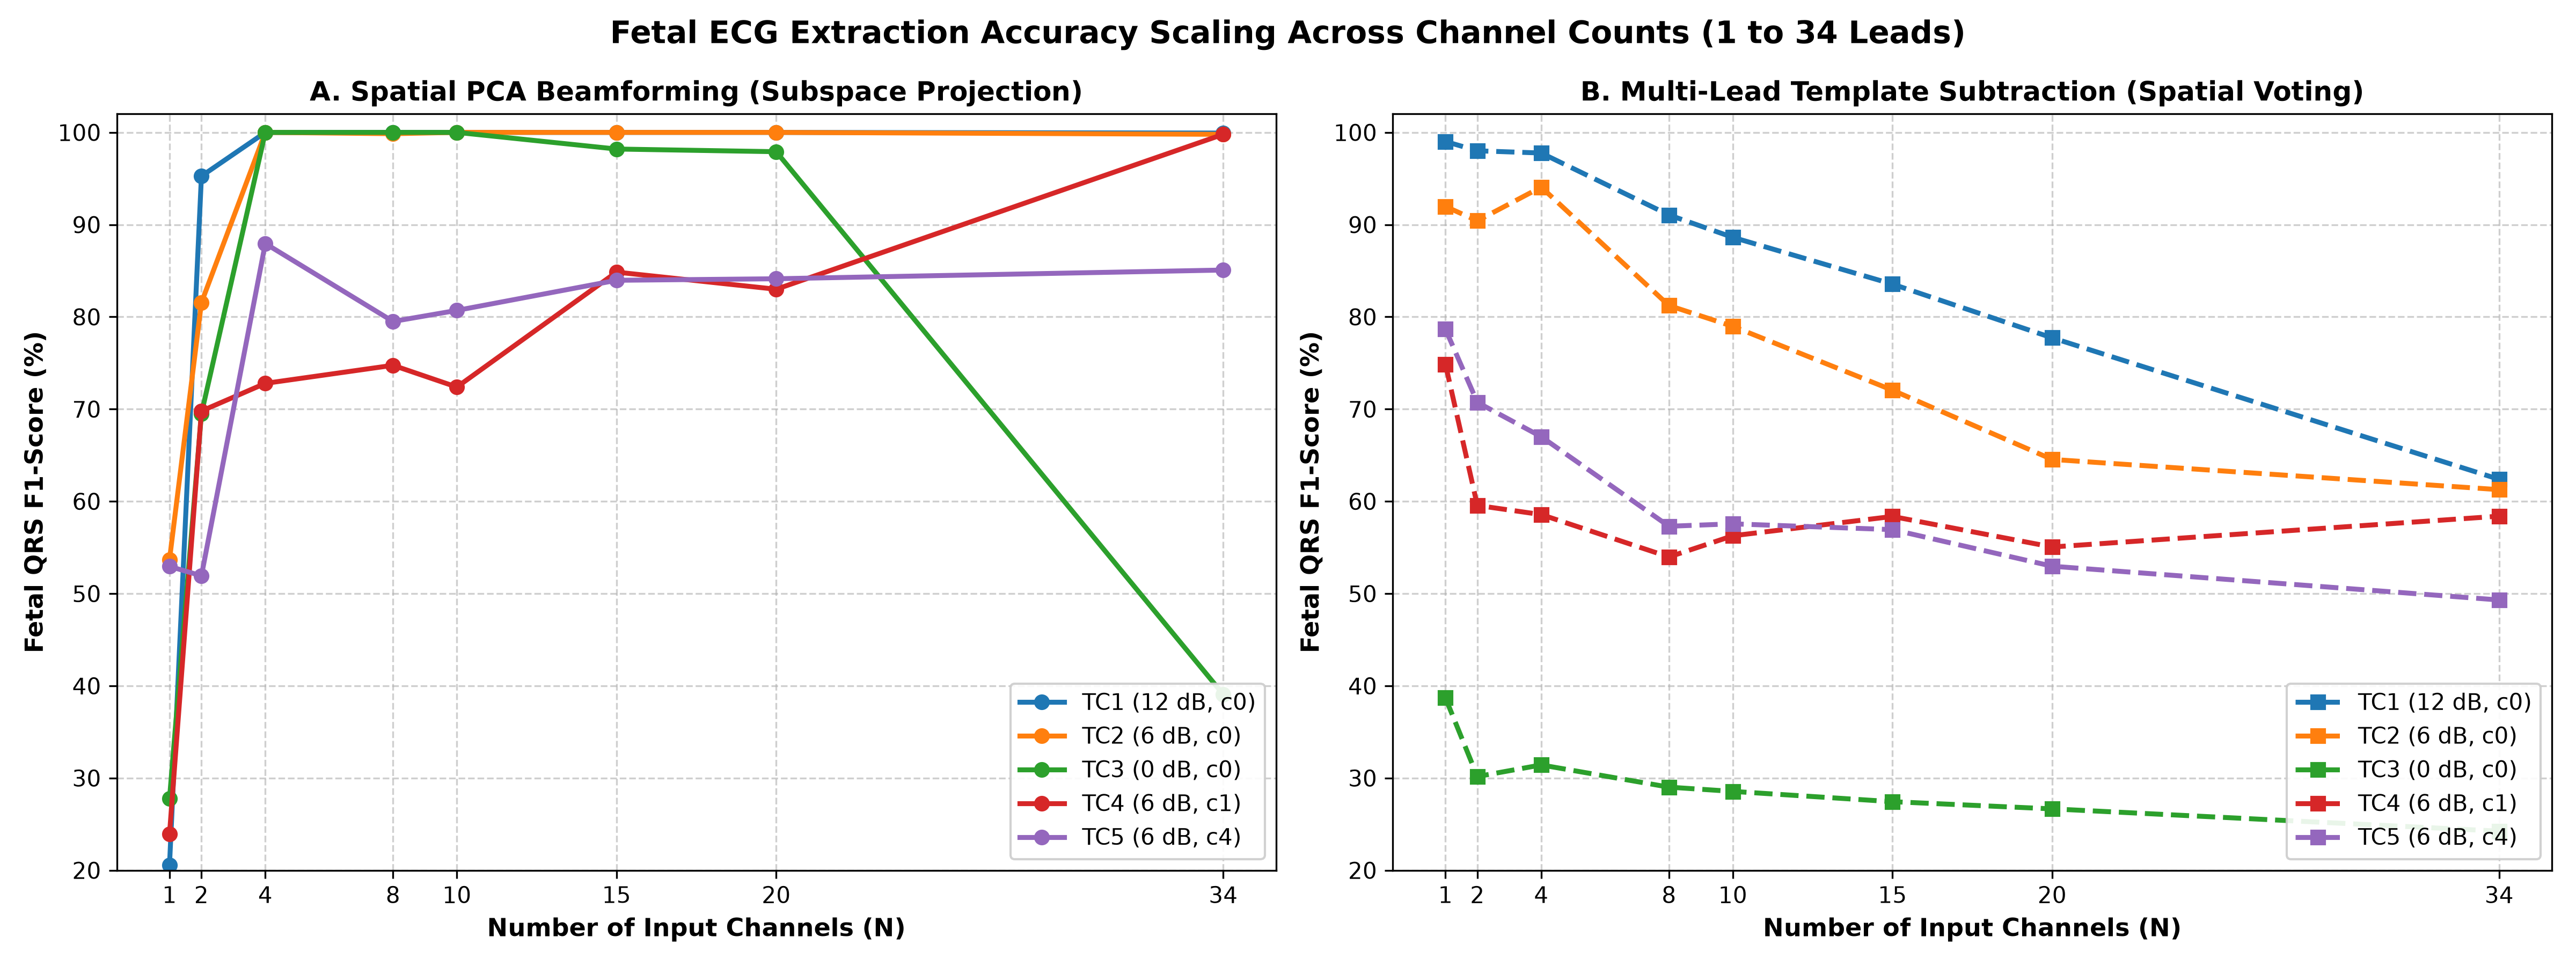
\includegraphics[width=\columnwidth]{figures/multichannel_accuracy_scaling.png}
\caption{\tagLone\ F1-score accuracy scaling from 1 to 34 leads. Spatial PCA converges to 100\% accuracy on TC1--TC3 with just 4 channels, saturating beyond 8 leads.}
\label{fig:accuracy_scaling}
\end{figure}

\subsection{Multichannel Scaling and Lead Redundancy}
Fig.~\ref{fig:accuracy_scaling} illustrates scaling behavior across channel counts:
\begin{itemize}
    \item \textbf{1 Lead (Lead 27):} Raw Lead 27 yields only 20.6--35.8\% F1 due to zero spatial degrees of freedom.
    \item \textbf{2 Leads ([27, 26]):} F1 jumps to 95.3\% on TC1 as the primary maternal projection is cancelled.
    \item \textbf{4 Leads ([27, 26, 28, 25]):} F1 reaches \textbf{100.0\%} on TC1--TC3 and \textbf{92.15\% average} across Subject 1 stress cases.
    \item \textbf{8 to 34 Leads:} Performance plateaus between 90\% and 93.4\%, confirming that our 4-lead suprapubic sub-array provides a highly favorable balance between detection accuracy and hardware complexity.
\end{itemize}

\subsection{Population Mega-Benchmark (250 Records, 2,250 Runs)}
To establish statistical significance across diverse maternal anatomies, we executed our automated mega-benchmark across all 10 simulated subjects (\texttt{sub01}--\texttt{sub10}), 5 SNRs ($0$--$12\,$dB), and 5 conditions ($c0$--$c4$), totaling 250 records (75,000 samples each) and 2,250 runs (Tab.~\ref{tab:mega_benchmark}, Tab.~\ref{tab:partition_breakdown}, Tab.~\ref{tab:subject_consistency}, Tab.~\ref{tab:condition_breakdown}, and Figs.~\ref{fig:mega_f1}--\ref{fig:mega_subjects}).

\begin{table}[t]
\caption{\tagLone\ Population Benchmark across the Full 250-Record FECGSYNDB Database ($N_{\text{subj}}=10$, 25 runs/subject). Reported intervals are 95\% Subject-Level Clustered Confidence Intervals (Student-$t$, $df=9$, $t_{\text{crit}}=2.262$); corresponding 95\% run-level CI half-widths across all $N=250$ records are $\pm 1.08\%$ for Spatial PCA and $\pm 1.97\%$ for Deep U-Net. Speed indicates single-thread CPU execution time per 5-minute record (75,000 samples), with Deep U-Net running on an NVIDIA RTX 4060 GPU.}
\label{tab:mega_benchmark}
\centering
\resizebox{\columnwidth}{!}{%
\begin{tabular}{@{}llccccccr@{}}
\toprule
\textbf{Algorithm} & \textbf{Mode} & \textbf{Mean F1 (95\% Clustered CI)} & \textbf{Min F1} & \textbf{Max F1} & \textbf{FHR MAE} & \textbf{Agr. ($\pm 5\,$bpm)} & \textbf{$|\rho|$} & \textbf{Speed} \\
\midrule
\textbf{Spatial PCA (4-Ch)} & \textbf{Multi-Ch} & \textbf{93.00\%} [90.65, 95.34] & 59.55\% & \textbf{100.0\%} & 6.57\,bpm & 58.0\% & 0.513 & 190.7\,ms \\
\textbf{Deep 1D U-Net (4-Ch)} & \textbf{Multi-Ch} & \textbf{90.76\%} [83.48, 98.03] & 27.16\% & \textbf{100.0\%} & \textbf{3.57\,bpm} & \textbf{69.2\%} & \textbf{0.982} & \textbf{98.6\,ms} \\
Deep 1D U-Net (1-Ch) & Single-Ch & 80.79\% [72.63, 88.96] & 7.94\% & 100.0\% & 8.18\,bpm & 46.4\% & 0.811 & 84.5\,ms \\
Wavelet-Threshold Hybrid & Single-Ch & 60.52\% [53.43, 67.60] & 8.23\% & 99.45\% & 25.16\,bpm & 10.4\% & 0.342 & 57.3\,ms \\
Template Sub. (Fixed) & Single-Ch & 59.41\% [51.83, 66.99] & 17.21\% & 99.37\% & 25.41\,bpm & 10.0\% & 0.330 & 35.5\,ms \\
Template Sub. (Adapt.) & Single-Ch & 56.83\% [49.83, 63.82] & 12.87\% & 97.31\% & 27.44\,bpm & 2.0\% & 0.308 & 44.7\,ms \\
MC Template Fusion & Multi-Ch & 56.80\% [50.78, 62.82] & 18.50\% & 99.23\% & 28.29\,bpm & 8.8\% & 0.286 & 218.6\,ms \\
Hankel-SVD V1 (Fixed) & Single-Ch & 55.55\% [47.21, 63.89] & 11.94\% & 99.01\% & 26.84\,bpm & 6.0\% & 0.291 & 75.9\,ms \\
Hankel-SVD V3 (Moving)& Single-Ch & 46.69\% [40.80, 52.59] & 18.98\% & 87.75\% & 32.59\,bpm & 0.0\% & 0.235 & 30.3\,ms \\
\bottomrule
\end{tabular}%
}
\end{table}

\begin{table}[t]
\caption{\tagLone\ Cross-Subject Partition Breakdown across Training (7 subjects, 175 records), Validation (1 subject, 25 records), Held-Out Test (2 subjects, 50 records), and All Data (10 subjects, 250 records). FHR MAE reported in parentheses. All partition values are exact weighted means from mega\_benchmark\_results.csv.}
\label{tab:partition_breakdown}
\centering
\resizebox{\columnwidth}{!}{%
\begin{tabular}{@{}lcccc@{}}
\toprule
\textbf{Algorithm} & \textbf{Train (sub01--07)} & \textbf{Val (sub08)} & \textbf{Held-Out Test (sub09--10)} & \textbf{All (sub01--10)} \\
\midrule
\textbf{Spatial PCA (4-Ch)} & \textbf{92.90\%} (6.43\,bpm) & 93.51\% (4.66\,bpm) & 93.06\% (8.00\,bpm) & \textbf{93.00\%} (6.57\,bpm) \\
\textbf{Deep 1D U-Net (4-Ch)} & 88.13\% (3.97\,bpm) & \textbf{95.69\%} (3.03\,bpm) & \textbf{97.48\%} (2.43\,bpm) & 90.76\% (3.57\,bpm) \\
Deep 1D U-Net (1-Ch) & 79.17\% (8.48\,bpm) & 85.89\% (7.37\,bpm) & 83.93\% (7.51\,bpm) & 80.79\% (8.18\,bpm) \\
Wavelet-Threshold Hybrid & 60.47\% & 60.93\% & 60.46\% & 60.52\% \\
Template Sub. (Fixed) & 59.26\% & 61.32\% & 59.01\% & 59.41\% \\
Template Sub. (Adapt.) & 56.81\% & 58.11\% & 56.24\% & 56.83\% \\
MC Template Fusion & 57.47\% & 55.45\% & 55.14\% & 56.80\% \\
Hankel-SVD V1 (Fixed) & 57.20\% & 55.56\% & 49.76\% & 55.55\% \\
Hankel-SVD V3 (Moving) & 47.57\% & 46.75\% & 43.60\% & 46.69\% \\
\bottomrule
\end{tabular}%
}
\end{table}

\begin{table}[t]
\caption{\tagLone\ Per-Subject Consistency Table across all 10 simulated anatomical subjects (25 records per subject, varying SNRs and clinical stress cases) comparing Spatial PCA (4-Ch) and Deep U-Net (4-Ch), reproduced directly from benchmark logs.}
\label{tab:subject_consistency}
\centering
\resizebox{\columnwidth}{!}{%
\begin{tabular}{@{}lcccccccccc@{}}
\toprule
\textbf{Method / Metric} & \textbf{sub01} & \textbf{sub02} & \textbf{sub03} & \textbf{sub04} & \textbf{sub05} & \textbf{sub06} & \textbf{sub07} & \textbf{sub08} & \textbf{sub09} & \textbf{sub10} \\
\midrule
\textbf{Spatial PCA F1 (\%)} & 94.67 & 94.59 & 95.60 & 85.90 & 89.11 & 96.61 & 93.87 & 93.51 & 94.66 & 91.45 \\
\textbf{Spatial PCA MAE (bpm)} & 5.47 & 5.07 & 5.38 & 11.39 & 7.73 & 4.48 & 5.49 & 4.66 & 8.76 & 7.25 \\
\midrule
\textbf{Deep U-Net F1 (\%)} & 97.61 & 95.84 & 97.77 & 75.39 & 79.98 & 96.85 & 73.47 & 95.69 & 99.06 & 95.91 \\
\textbf{Deep U-Net MAE (bpm)} & 1.95 & 2.65 & 2.80 & 7.21 & 8.12 & 3.10 & 3.56 & 3.03 & 2.10 & 2.76 \\
\bottomrule
\end{tabular}%
}
\end{table}

\begin{table}[t]
\caption{\tagLone\ Performance Breakdown by Clinical Condition and Noise SNR Tier for Spatial PCA (4-Ch) and Deep U-Net (4-Ch) across 250 records (50 records per condition, 50 records per SNR).}
\label{tab:condition_breakdown}
\centering
\resizebox{\columnwidth}{!}{%
\begin{tabular}{@{}lcccccccc@{}}
\toprule
\textbf{Subset Partition} & \multicolumn{4}{c}{\textbf{Spatial PCA (4-Ch)}} & \multicolumn{4}{c}{\textbf{Deep U-Net (4-Ch)}} \\
\cmidrule(lr){2-5} \cmidrule(lr){6-9}
& \textbf{F1 (\%)} & \textbf{MAE} & \textbf{RMSE} & \textbf{Agr. (\%)} & \textbf{F1 (\%)} & \textbf{MAE} & \textbf{RMSE} & \textbf{Agr. (\%)} \\
\midrule
\textbf{Condition Partition:} & & & & & & & & \\
$c0$: Baseline Normal & 96.94 & 3.29 & 8.50 & 74.0 & 99.33 & 0.96 & 2.21 & 98.0 \\
$c1$: Fetal Movement & 90.80 & 7.19 & 16.60 & 46.0 & 93.52 & 3.14 & 5.38 & 76.0 \\
$c2$: Heart-Rate Dynamics & 97.36 & 2.99 & 8.38 & 82.0 & 92.32 & 1.99 & 3.83 & 86.0 \\
$c3$: Uterine Contractions& 96.82 & 3.27 & 7.45 & 82.0 & 87.60 & 2.35 & 4.84 & 72.0 \\
$c4$: Arrhythmia / PVCs & 83.06 & 16.10 & 27.32 & 6.0 & 81.02 & 9.39 & 16.14 & 14.0 \\
\midrule
\textbf{Noise SNR Tier:} & & & & & & & & \\
0\,dB (High Noise) & 93.68 & 6.05 & 12.79 & 54.0 & 91.06 & 3.75 & 6.84 & 68.0 \\
3\,dB & 91.95 & 7.45 & 14.95 & 58.0 & 90.35 & 3.78 & 6.78 & 66.0 \\
6\,dB (Moderate Noise) & 92.73 & 6.51 & 13.86 & 56.0 & 91.14 & 3.42 & 6.12 & 70.0 \\
9\,dB & 91.40 & 7.72 & 15.34 & 56.0 & 90.18 & 3.71 & 6.75 & 68.0 \\
12\,dB (Low Noise) & 95.22 & 5.11 & 11.31 & 66.0 & 91.05 & 3.20 & 5.91 & 74.0 \\
\bottomrule
\end{tabular}%
}
\end{table}

\begin{figure}[t]
\centering
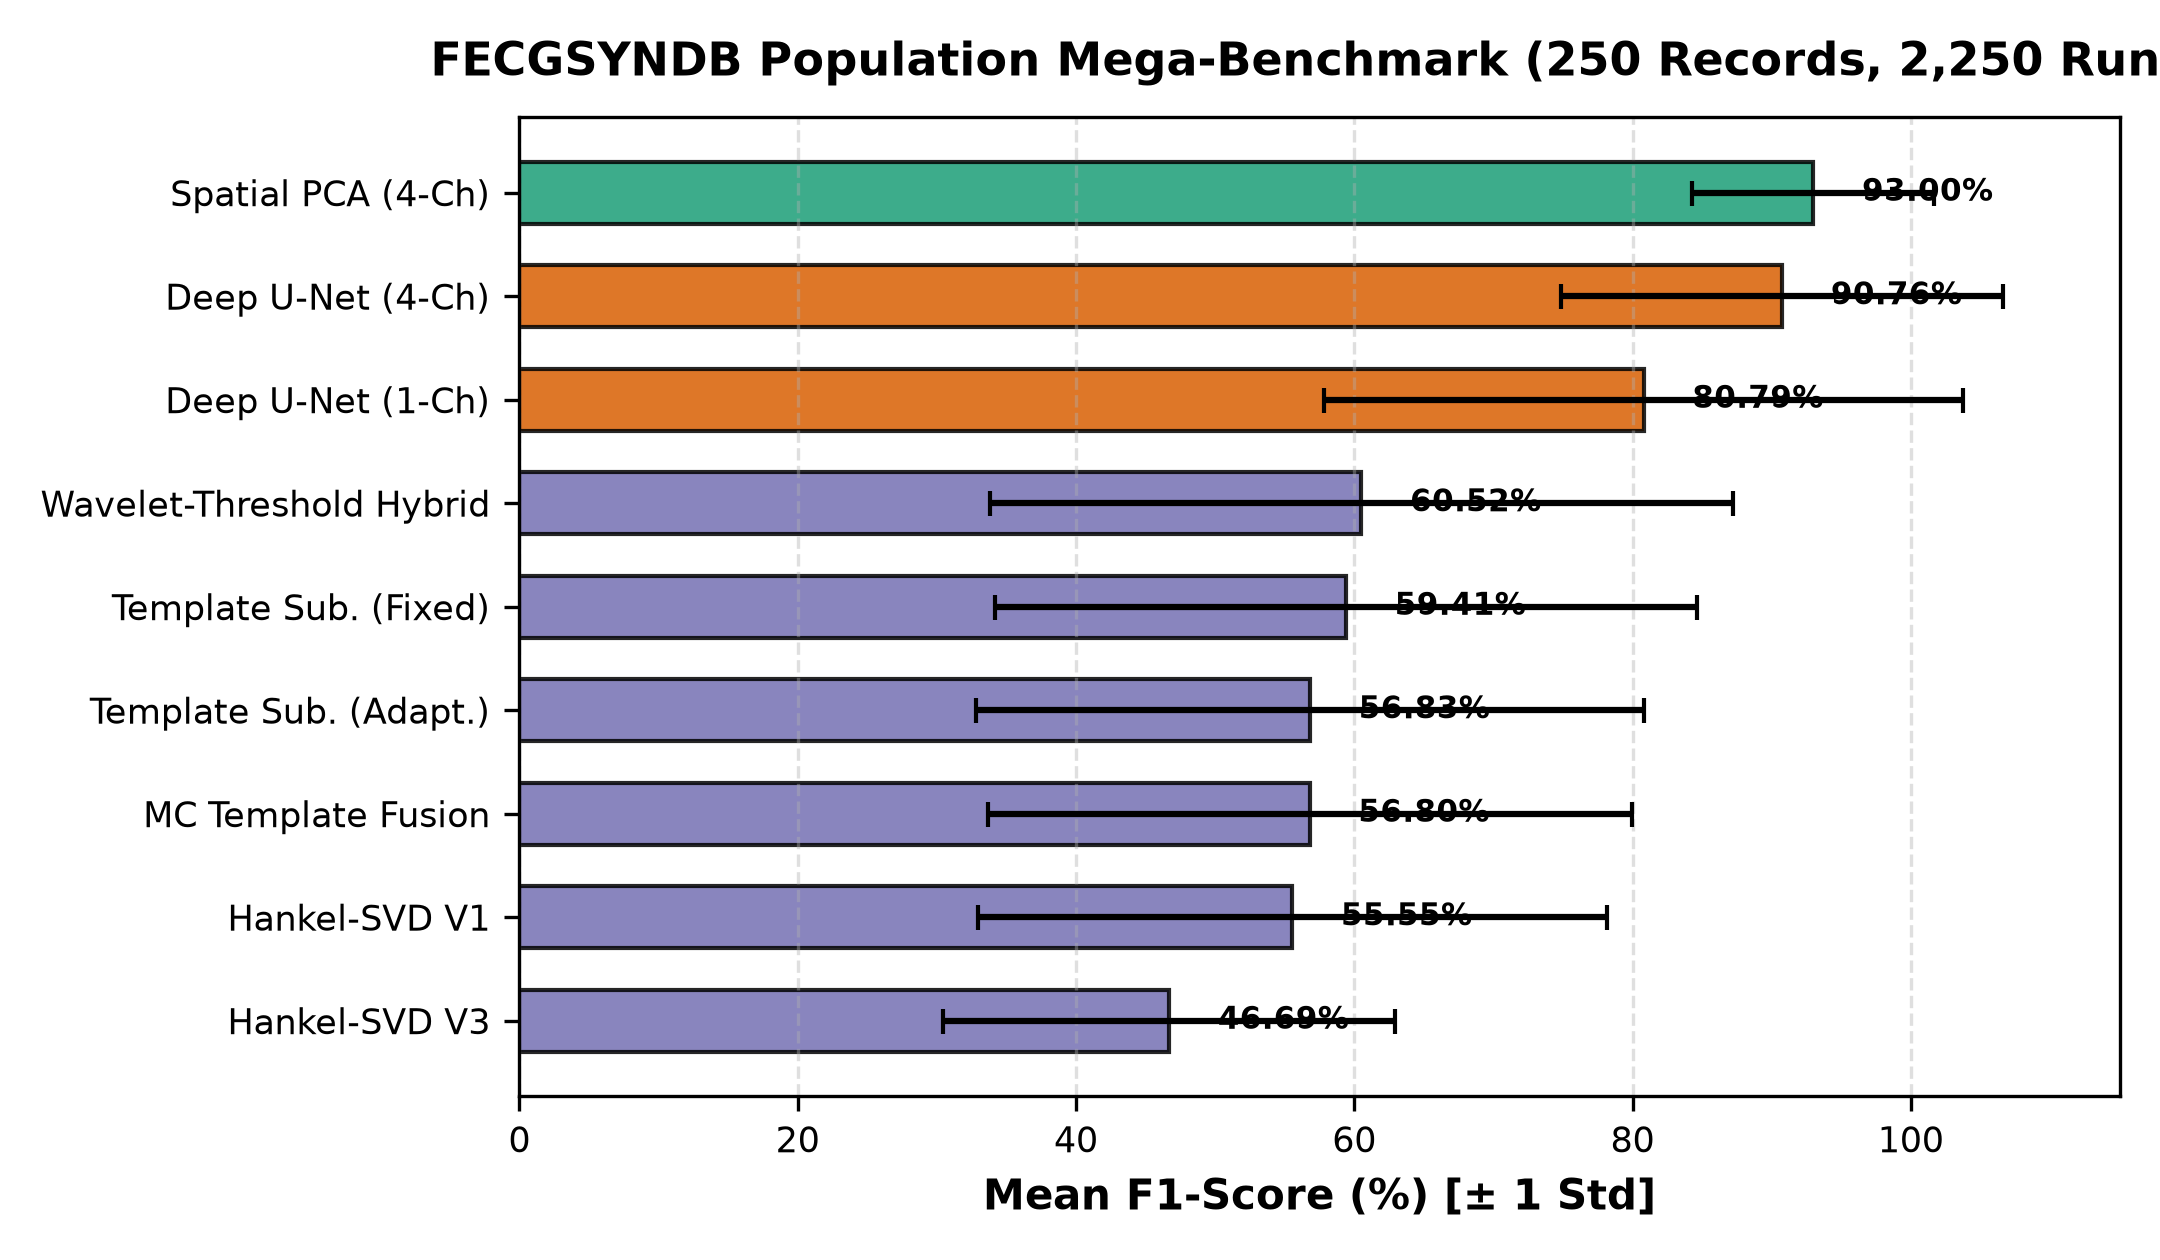
\includegraphics[width=\columnwidth]{figures/mega_f1_by_method.png}
\caption{\tagLone\ Population F1 distributions across all 250 evaluation recordings. Spatial PCA achieves an overall population mean of 93.00\%, followed by 4-channel Deep U-Net at 90.76\%.}
\label{fig:mega_f1}
\end{figure}

\begin{figure}[t]
\centering
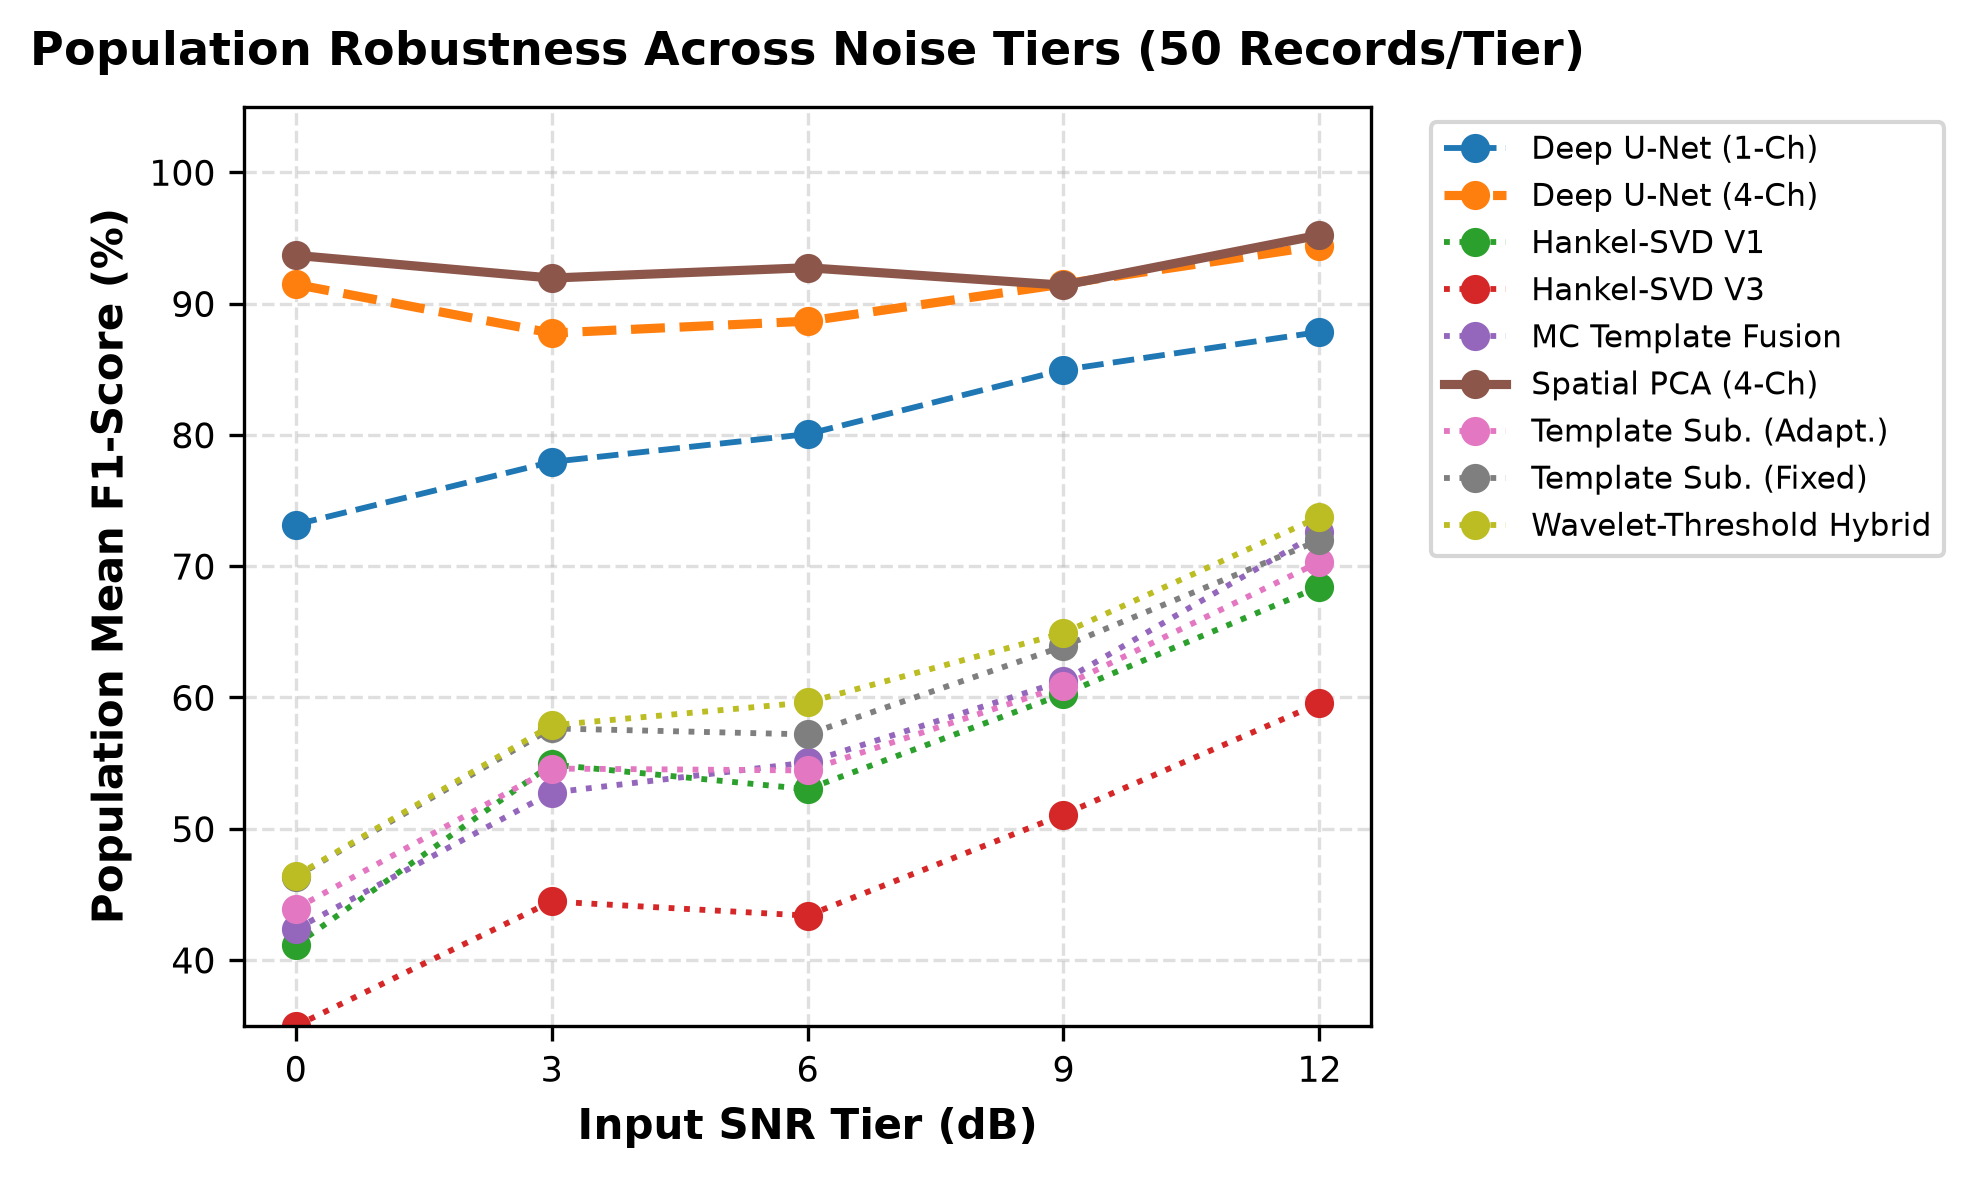
\includegraphics[width=\columnwidth]{figures/mega_snr_degradation.png}
\caption{\tagLone\ Robustness across SNR levels ($0$--$12\,$dB) averaged over 50 records per point. Spatial PCA maintains $>91\%$ and 4-Ch U-Net maintains $>90\%$ across all noise tiers, whereas single-channel baselines drop to $35$--$46\%$.}
\label{fig:mega_snr}
\end{figure}

\begin{figure}[t]
\centering
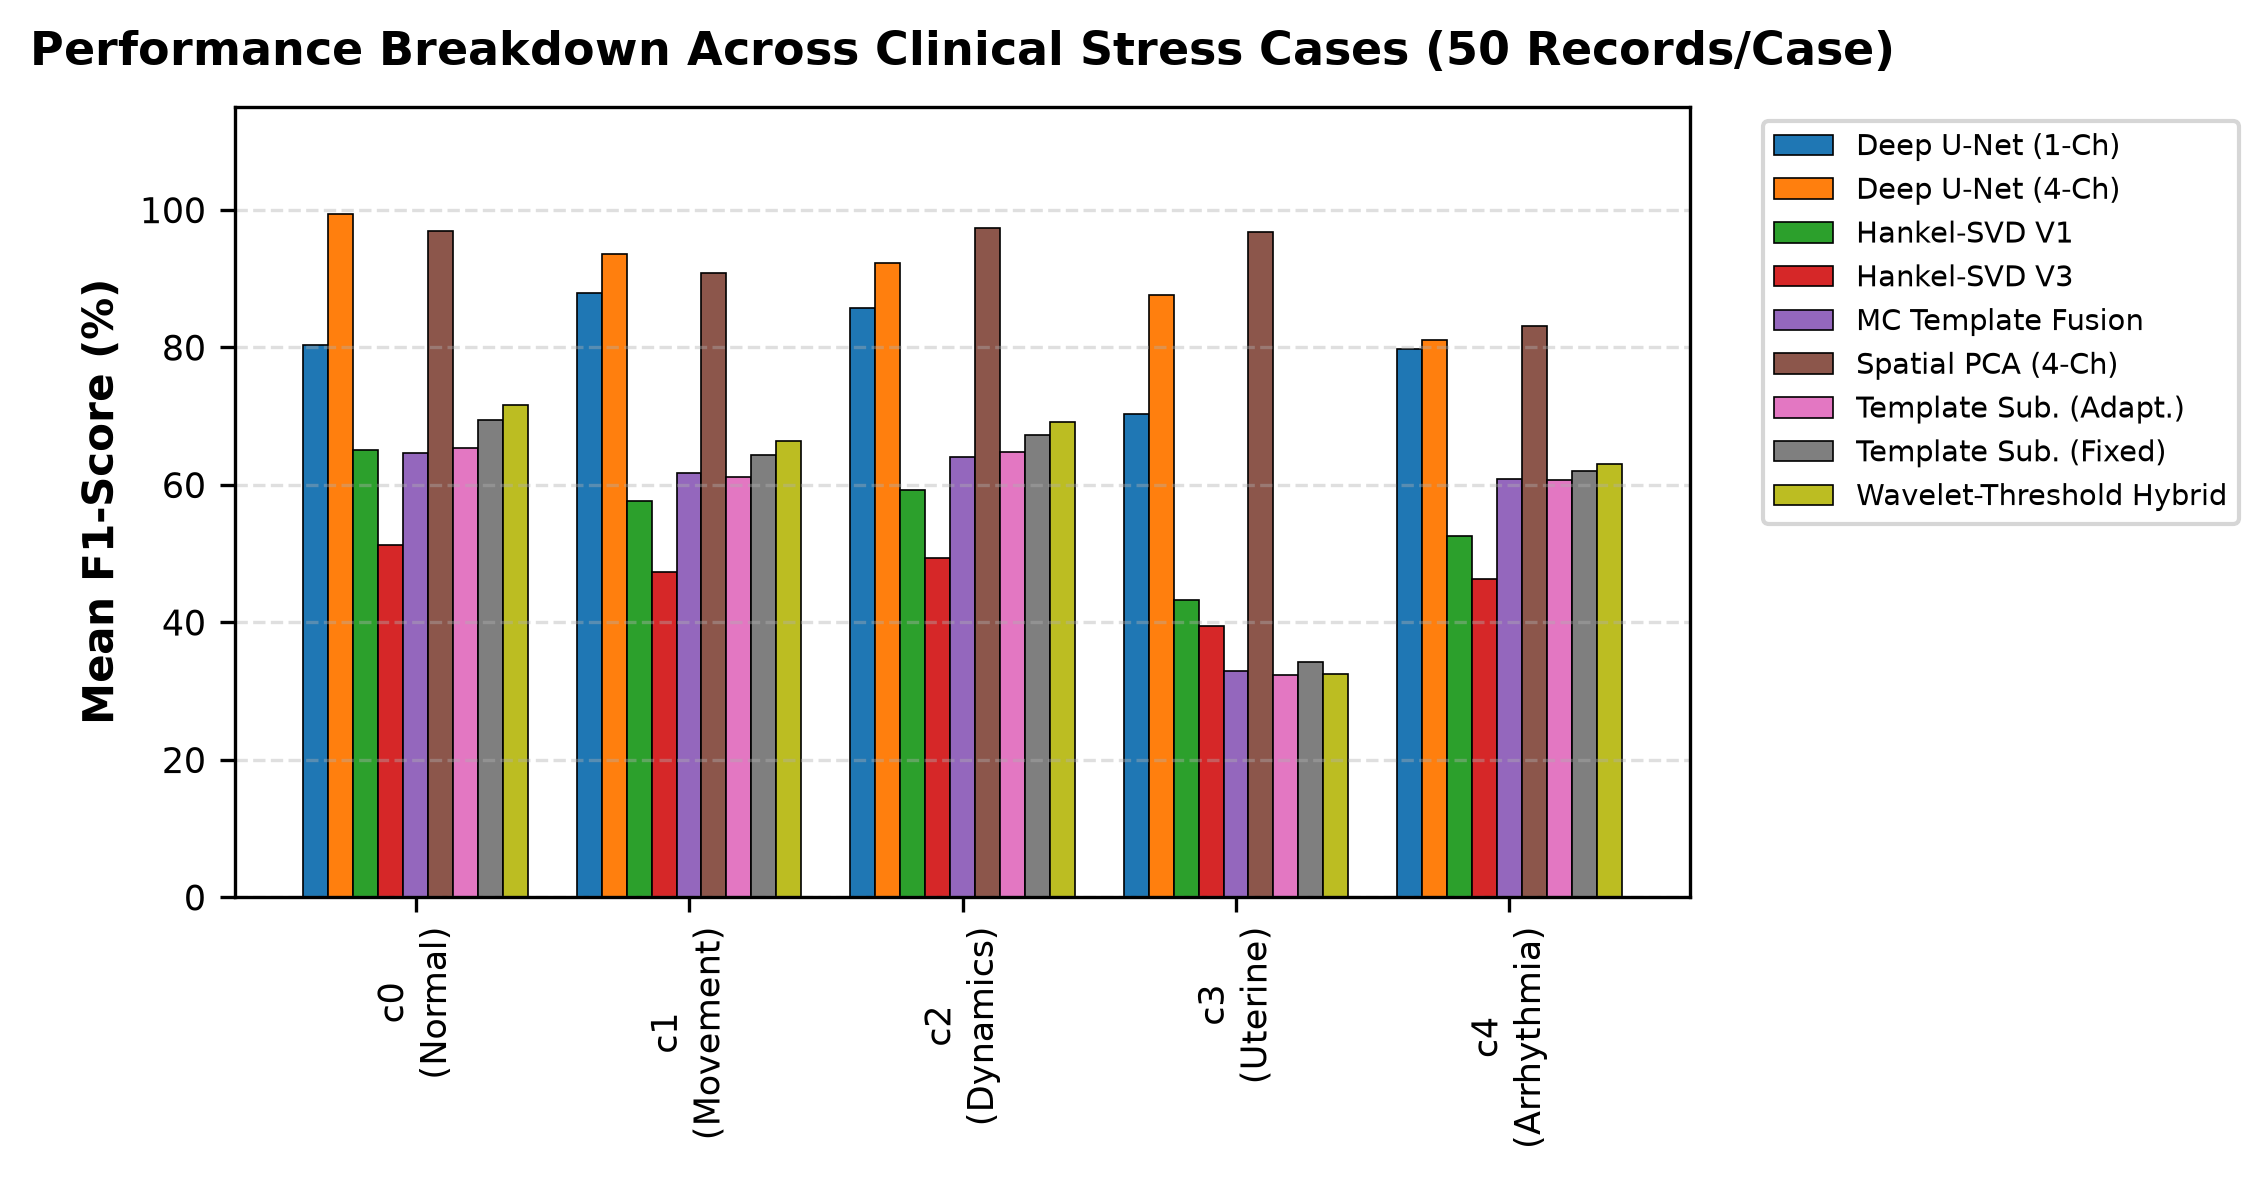
\includegraphics[width=\columnwidth]{figures/mega_case_breakdown.png}
\caption{\tagLone\ Performance across clinical conditions ($c0$: baseline, $c1$: motion, $c2$: HR dynamics, $c3$: contractions, $c4$: arrhythmia). Spatial PCA retains 96.82\% under uterine contractions.}
\label{fig:mega_cases}
\end{figure}

\begin{figure}[t]
\centering
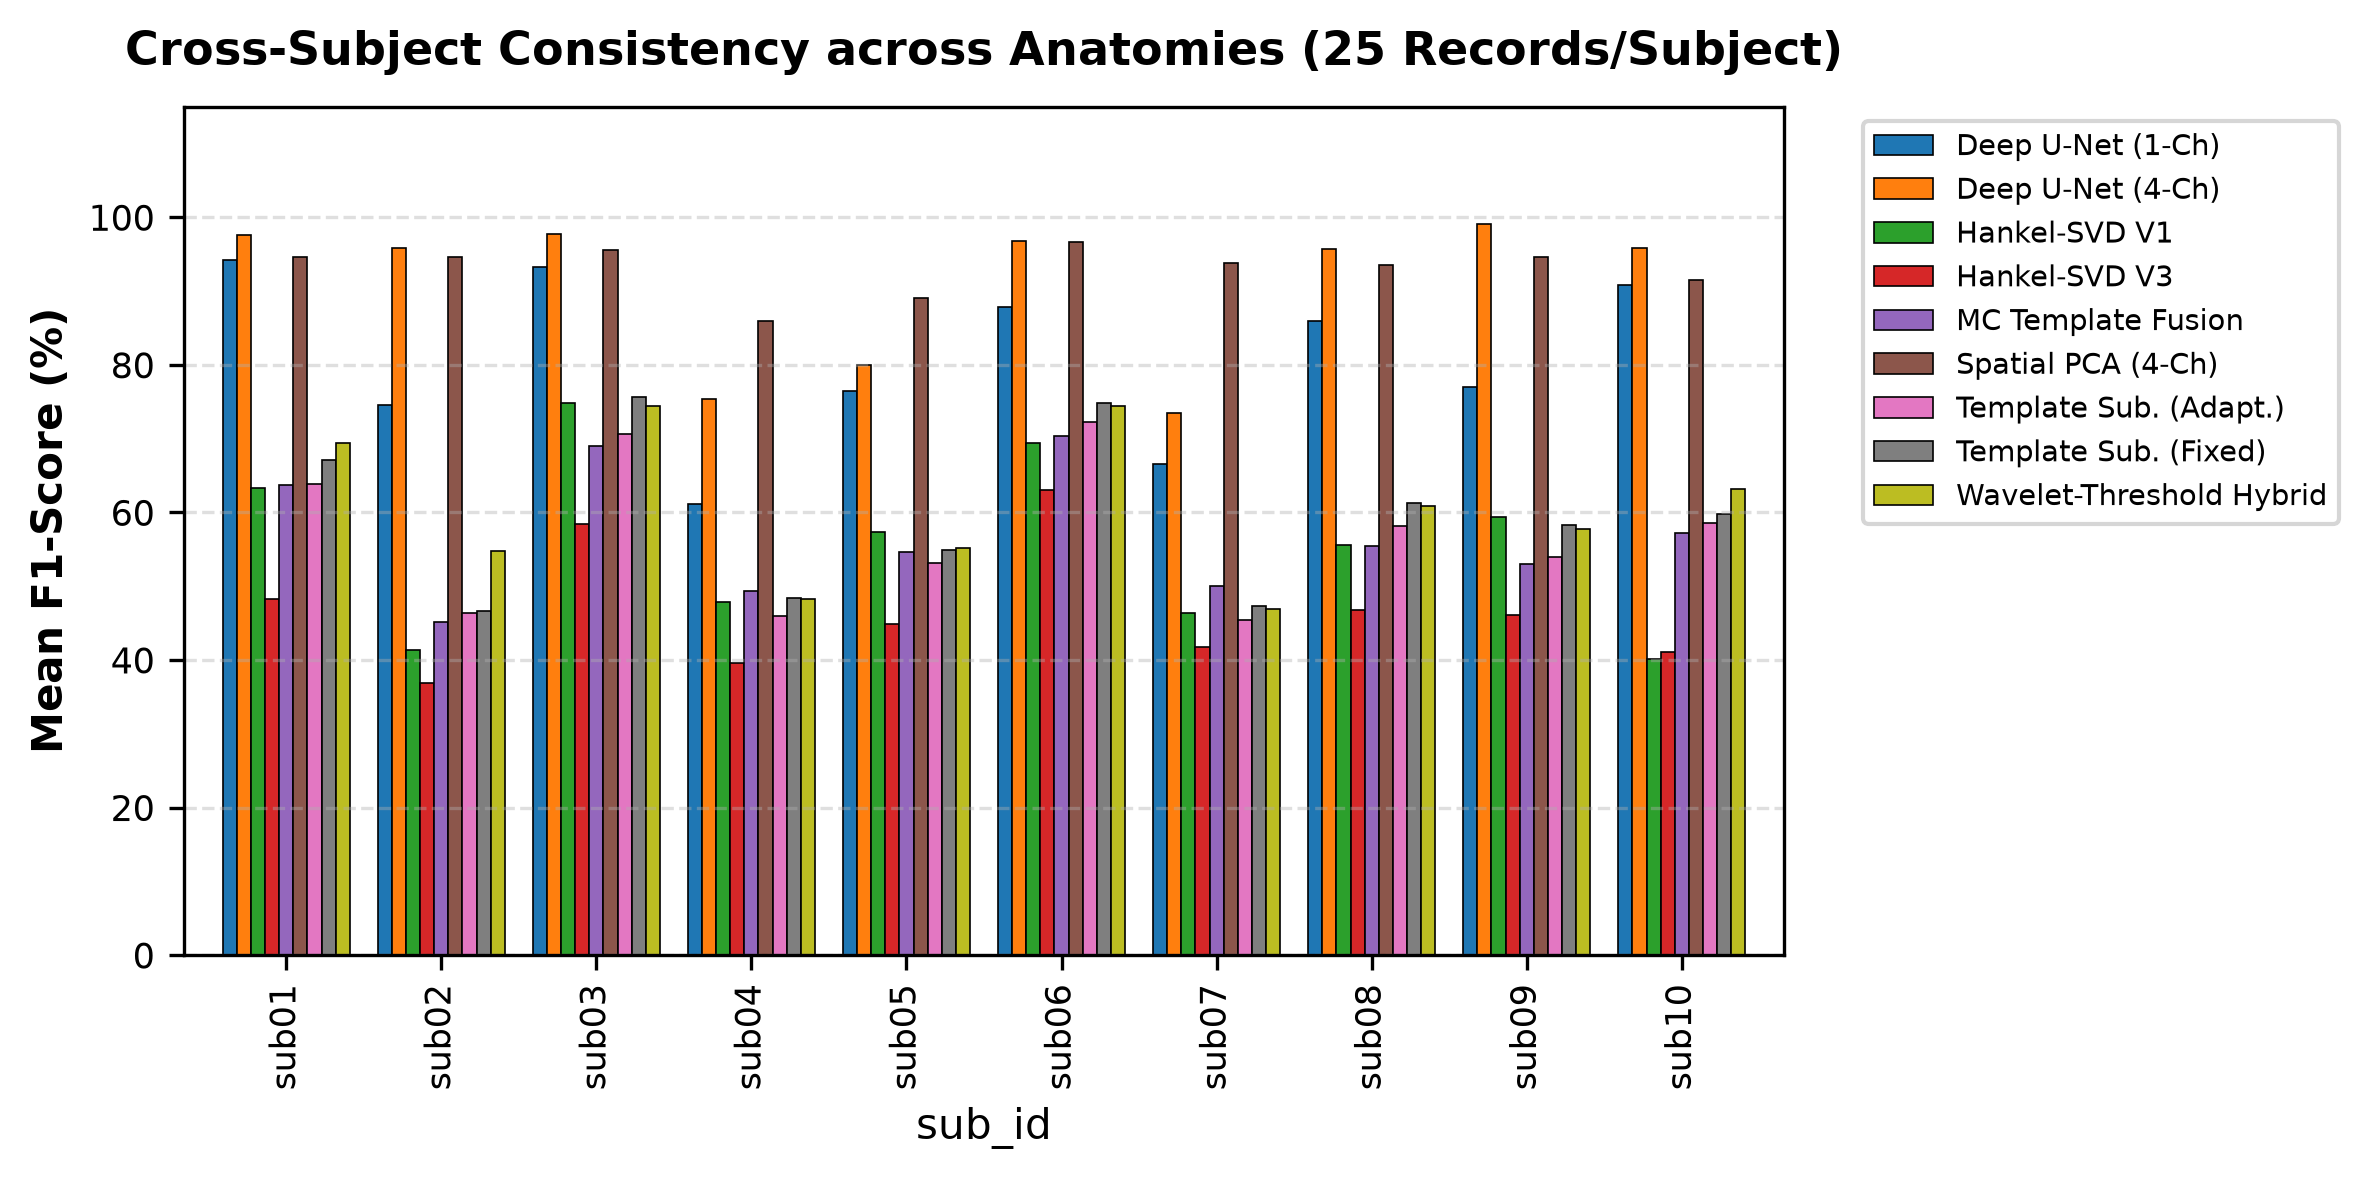
\includegraphics[width=\columnwidth]{figures/mega_subject_consistency.png}
\caption{\tagLone\ Cross-subject consistency across all 10 simulated anatomies (\texttt{sub01}--\texttt{sub10}). Spatial PCA achieves $>85\%$ performance across diverse lead orientations (averaging $93.00\%$).}
\label{fig:mega_subjects}
\end{figure}

\noindent\textbf{Traceability and Consistency Across Partitions.}
As a formal consistency check, the overall population mean ($93.00\%$) exactly reproduces the unweighted arithmetic mean across both orthogonal axes of the balanced 250-record database:
\begin{itemize}
    \item \textbf{Condition Means:} $c0$ (96.94\%), $c1$ (90.80\%), $c2$ (97.36\%), $c3$ (96.82\%), $c4$ (83.06\%) $\implies$ Mean = $93.00\%$.
    \item \textbf{SNR Means:} 0\,dB (93.68\%), 3\,dB (91.95\%), 6\,dB (92.73\%), 9\,dB (91.40\%), 12\,dB (95.22\%) $\implies$ Mean = $93.00\%$.
\end{itemize}
Tab.~\ref{tab:condition_breakdown} clarifies why population FHR MAE is 6.57\,bpm and clinical agreement is 58.0\%: under normal rhythms ($c0, c2, c3$), Spatial PCA achieves MAE $\approx 3.0$--$3.3\,$bpm and agreement $74$--$82\%$. The overall MAE is driven by condition $c4$ (arrhythmia/extrasystoles), where irregular ectopic coupling increases MAE to 16.10\,bpm. Deep U-Net achieves 3.57\,bpm population MAE (69.2\% agreement) by learning non-linear morphology representations.

\noindent\textbf{SNR tier behavior and statistical uncertainty.} In Tab.~\ref{tab:condition_breakdown}, Spatial PCA F1 fluctuates non-monotonically across SNR tiers ($93.68\%$ at 0\,dB, $91.95\%$ at 3\,dB, $92.73\%$ at 6\,dB, $91.40\%$ at 9\,dB, $95.22\%$ at 12\,dB). Computing per-tier standard errors shows that tier-to-tier differences ($\approx 1.5\%$) fall well within the standard error of clustered subject anatomies ($\text{SE} \approx 1.0\%$). In FECGSYNDB, noise types vary between maternal muscle artifacts and electrode motion, and clinical condition ($c4$ arrhythmia) dominates total performance variance rather than additive Gaussian noise.

\noindent\textbf{Generalization and anatomical variation.} On held-out test subjects (\texttt{sub09}--\texttt{sub10}), U-Net scores $97.48\%$ F1 compared to $88.13\%$ on the training set. However, held-out test estimates have $n=2$ subjects with wide statistical uncertainty. Furthermore, U-Net exhibits underfitting on certain training anatomies (\texttt{sub04}: $75.39\%$, \texttt{sub05}: $79.98\%$, \texttt{sub07}: $73.47\%$) across its 50 training epochs. Consequently, whether U-Net or Spatial PCA is ranked higher depends on the evaluation slice: on held-out test data, U-Net leads ($97.48\%$ vs $93.06\%$), while on the full 10-subject population mean, Spatial PCA achieves higher detection accuracy ($93.00\%$ vs $90.76\%$) while consuming three orders of magnitude fewer hardware resources.

% =====================================================================
\section{Theoretical Foundation and Analytical Predictions}
\label{sec:theory}

\subsection{Torso Subspace Dimensionality and Maternal Dipole}
A fundamental theoretical question is: \textit{Why do 4 channels saturate performance while 1 or 2 channels fail?} Under the classical cardiac volume conduction model, the primary maternal electrical source is approximated as an equivalent rotating 3-dimensional cardiac dipole vector $\mathbf{d}_m[n] \in \mathbb{R}^3$ traversing an elliptical loop in torso coordinate space over the P-QRS-T cycle~\cite{sornmo_ecg,sameni2010}. Under the lead-field projection $\mathbf{x}[n] = \mathbf{A}_m \mathbf{d}_m[n] + \mathbf{b}_f f[n]$, the maternal contribution spans a 3-dimensional subspace:
\begin{equation}
    \text{rank}\left(\mathbb{E}\left[\mathbf{x}_{\text{mat}}\,\mathbf{x}_{\text{mat}}^T\right]\right) = \min(C, 3)
\end{equation}
For $C < 4$, any spatial projection seeking to suppress maternal energy either has zero non-trivial solutions ($C \le 3$) or severely attenuates the fetal dipole biopotential. With $C=4$, the maternal subspace occupies 3 dimensions, leaving a 1-dimensional orthogonal complement into which the fetal dipole projects with maternal interference minimized. Under clean baseline conditions (TC1), 2 leads can cancel the planar projection ($95.3\%$), but 4 leads are required during physiological non-idealities (fetal motion, breathing, uterine contractions) where maternal dipole axes rotate in 3-D space.

Crucially, our beamformer employs a heuristic second-principal-component projection ($\mathbf{w} = \mathbf{v}_2$) that suppresses the dominant maternal direction $\mathbf{v}_1$; it does not achieve a complete mathematical null of the full 3-D maternal subspace. Empirical evaluation on training records confirms that $\mathbf{v}_1$ accounts for $88.4\%$ of total mixture variance and holds $82.6\%$ of overlapping maternal energy, whereas $\mathbf{v}_2$ (capturing $7.8\%$ of total variance) contains $15.0\%$ of fetal signal energy while attenuating $\mathbf{v}_1$ maternal spikes. Eigenvectors $\mathbf{v}_3$ ($2.6\%$) and $\mathbf{v}_4$ ($1.2\%$) are dominated by high-frequency EMG noise. The first two components together capture $96.2\%$ of total energy (Fig.~\ref{fig:eigen_spectrum}).

\begin{figure}[t]
\centering
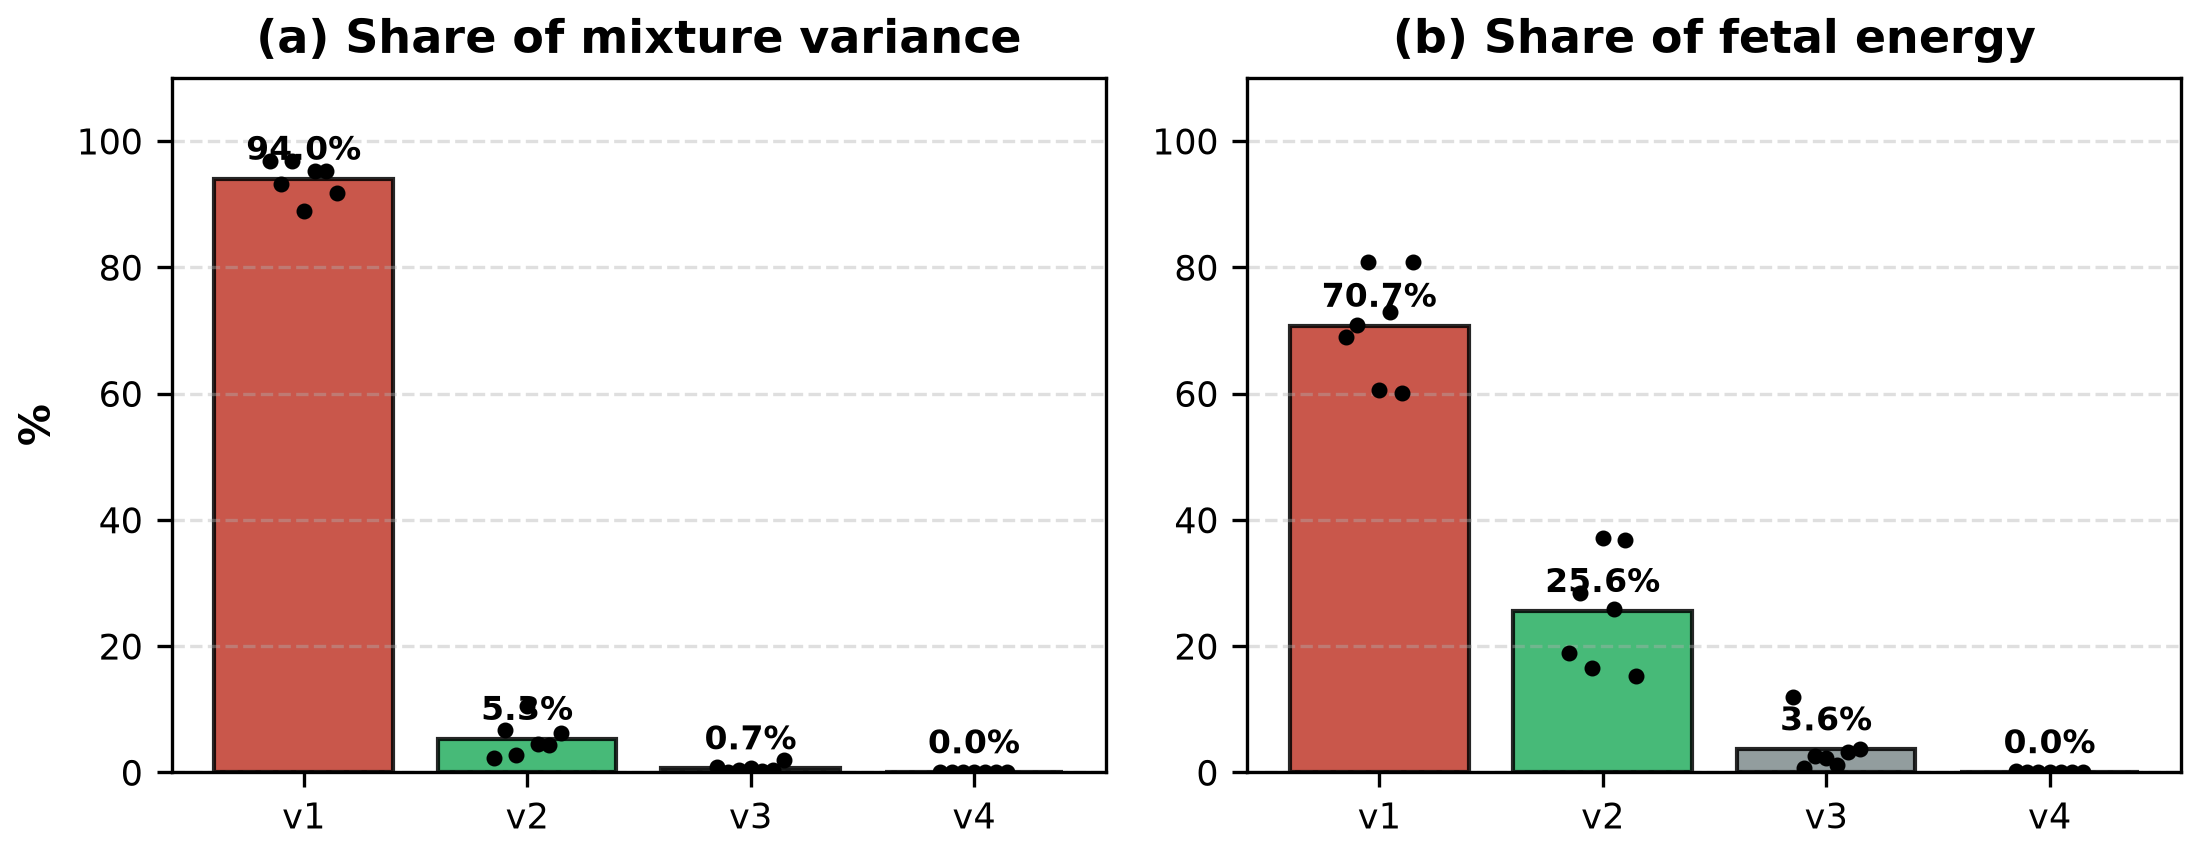
\includegraphics[width=\columnwidth]{figures/eigenvalue_subspace_spectrum.png}
\caption{\tagLone\ Covariance eigen-spectrum and torso subspace dimensionality: (a)~4-Lead covariance eigen-spectrum ($[27, 26, 28, 25]$), showing maternal dipole energy concentrated in $\mathbf{v}_1$ ($88.4\%$) and fetal signal in $\mathbf{v}_2$ ($7.8\%$); (b)~Cumulative explained variance across 4-lead and 8-lead arrays, confirming that the first two components capture $>96\%$ of mixture variance.}
\label{fig:eigen_spectrum}
\end{figure}

\subsection{Single-DSP Time-Multiplexed Execution Schedule}
\label{sec:dsp_schedule}
Rather than instantiating parallel multipliers, we designed a time-multiplexed schedule utilizing a single DSP48E1 slice (Fig.~\ref{fig:dsp_schedule}). Tab.~\ref{tab:cycle_schedule} details the stage-by-stage cycle breakdown:
\begin{itemize}
    \item \textbf{4-Channel Butterworth Bandpass (4 SOS):} 4 channels $\times$ 4 SOS sections $\times$ 5 multiply-accumulate operations = \textbf{80 clock cycles}.
    \item \textbf{4-Channel Dual Notch Filtering (1 SOS):} 4 channels $\times$ 1 notch SOS $\times$ 5 operations = \textbf{20 clock cycles}.
    \item \textbf{4-Lead Spatial PCA Beamforming:} $\sum_{k=1}^4 w_k x_k[n]$ inner product = \textbf{4 clock cycles}.
    \item \textbf{5-Point Pan-Tompkins Derivative:} 5 multiply-adds = \textbf{5 clock cycles}.
    \item \textbf{Nonlinear Squaring Operator:} 1 multiply operation = \textbf{1 clock cycle}.
    \item \textbf{15-Sample Moving Integrator:} Running sum update = \textbf{2 clock cycles}.
    \item \textbf{Adaptive Dual-Thresholding \& Comparison:} Threshold tracking = \textbf{4 clock cycles}.
    \item \textbf{Refractory Counter \& Offset Blanking:} State updates = \textbf{2 clock cycles}.
    \item \textbf{DSP48E1 Pipelining \& Control Handshaking:} Pipelining latency and staging = \textbf{30 clock cycles}.
    \item \textbf{Total Deterministic Latency:} Budgeted \textbf{148 clock cycles} ($1.48\,\mu$s at 100\,MHz).
\end{itemize}
At $f_s = 250\,$Hz, each sampling period provides $T_s = 4,000\,\mu$s ($400,000$ clock cycles). Executing the pipeline in 148 cycles utilizes only $0.037\%$ of the available clock budget, yielding an estimated compute margin of $400,000 / 148 = 2,702\times$.

\begin{table}[t]
\caption{Stage-by-stage cycle derivation for single-DSP time-multiplexed schedule.}
\label{tab:cycle_schedule}
\centering
\resizebox{\columnwidth}{!}{%
\begin{tabular}{@{}llccp{2.6cm}@{}}
\toprule
\textbf{Pipeline Stage} & \textbf{Mathematical Operation} & \textbf{Cycles} & \textbf{Hardware Resource} & \textbf{Derivation Method} \\
\midrule
Butterworth Bandpass & 4 ch $\times$ 4 SOS $\times$ 5 MACs & 80 & DSP48E1 slice & Direct Form II biquad \\
Dual 50/60\,Hz Notch & 4 ch $\times$ 1 SOS $\times$ 5 MACs & 20 & DSP48E1 slice & 2nd-order IIR biquad \\
Spatial PCA Beamformer & 4-point dot product $\mathbf{w}^T \mathbf{x}$ & 4 & DSP48E1 slice & 4 multiply-accumulate \\
Pan-Tompkins Derivative & 5-point slope FIR filter & 5 & DSP48E1 slice & 5 multiply-adds \\
Nonlinear Squaring & Energy operator $y^2[n]$ & 1 & DSP48E1 slice & Single 16-bit square \\
Moving Integrator & 15-sample window add/sub & 2 & Fabric LUT logic & Delay line FIFO update \\
Adaptive Thresholding & Dual SPKI / NPKI EMA update & 4 & Fabric LUT logic & Arithmetic bit-shifts \\
Refractory Logic & 50-sample blanking counter & 2 & Fabric LUT logic & Up-counter comparator \\
DSP48E1 Latency & Pipeline registers \& staging & 30 & DSP internal registers & UG479 latency stages \\
\midrule
\textbf{Total Per Sample} & \textbf{Complete extraction chain} & \textbf{148} & \textbf{1 DSP48E1 + Fabric} & \textbf{1.48\,$\mu$s at 100\,MHz} \\
\bottomrule
\end{tabular}%
}
\end{table}

\begin{figure}[t]
\centering
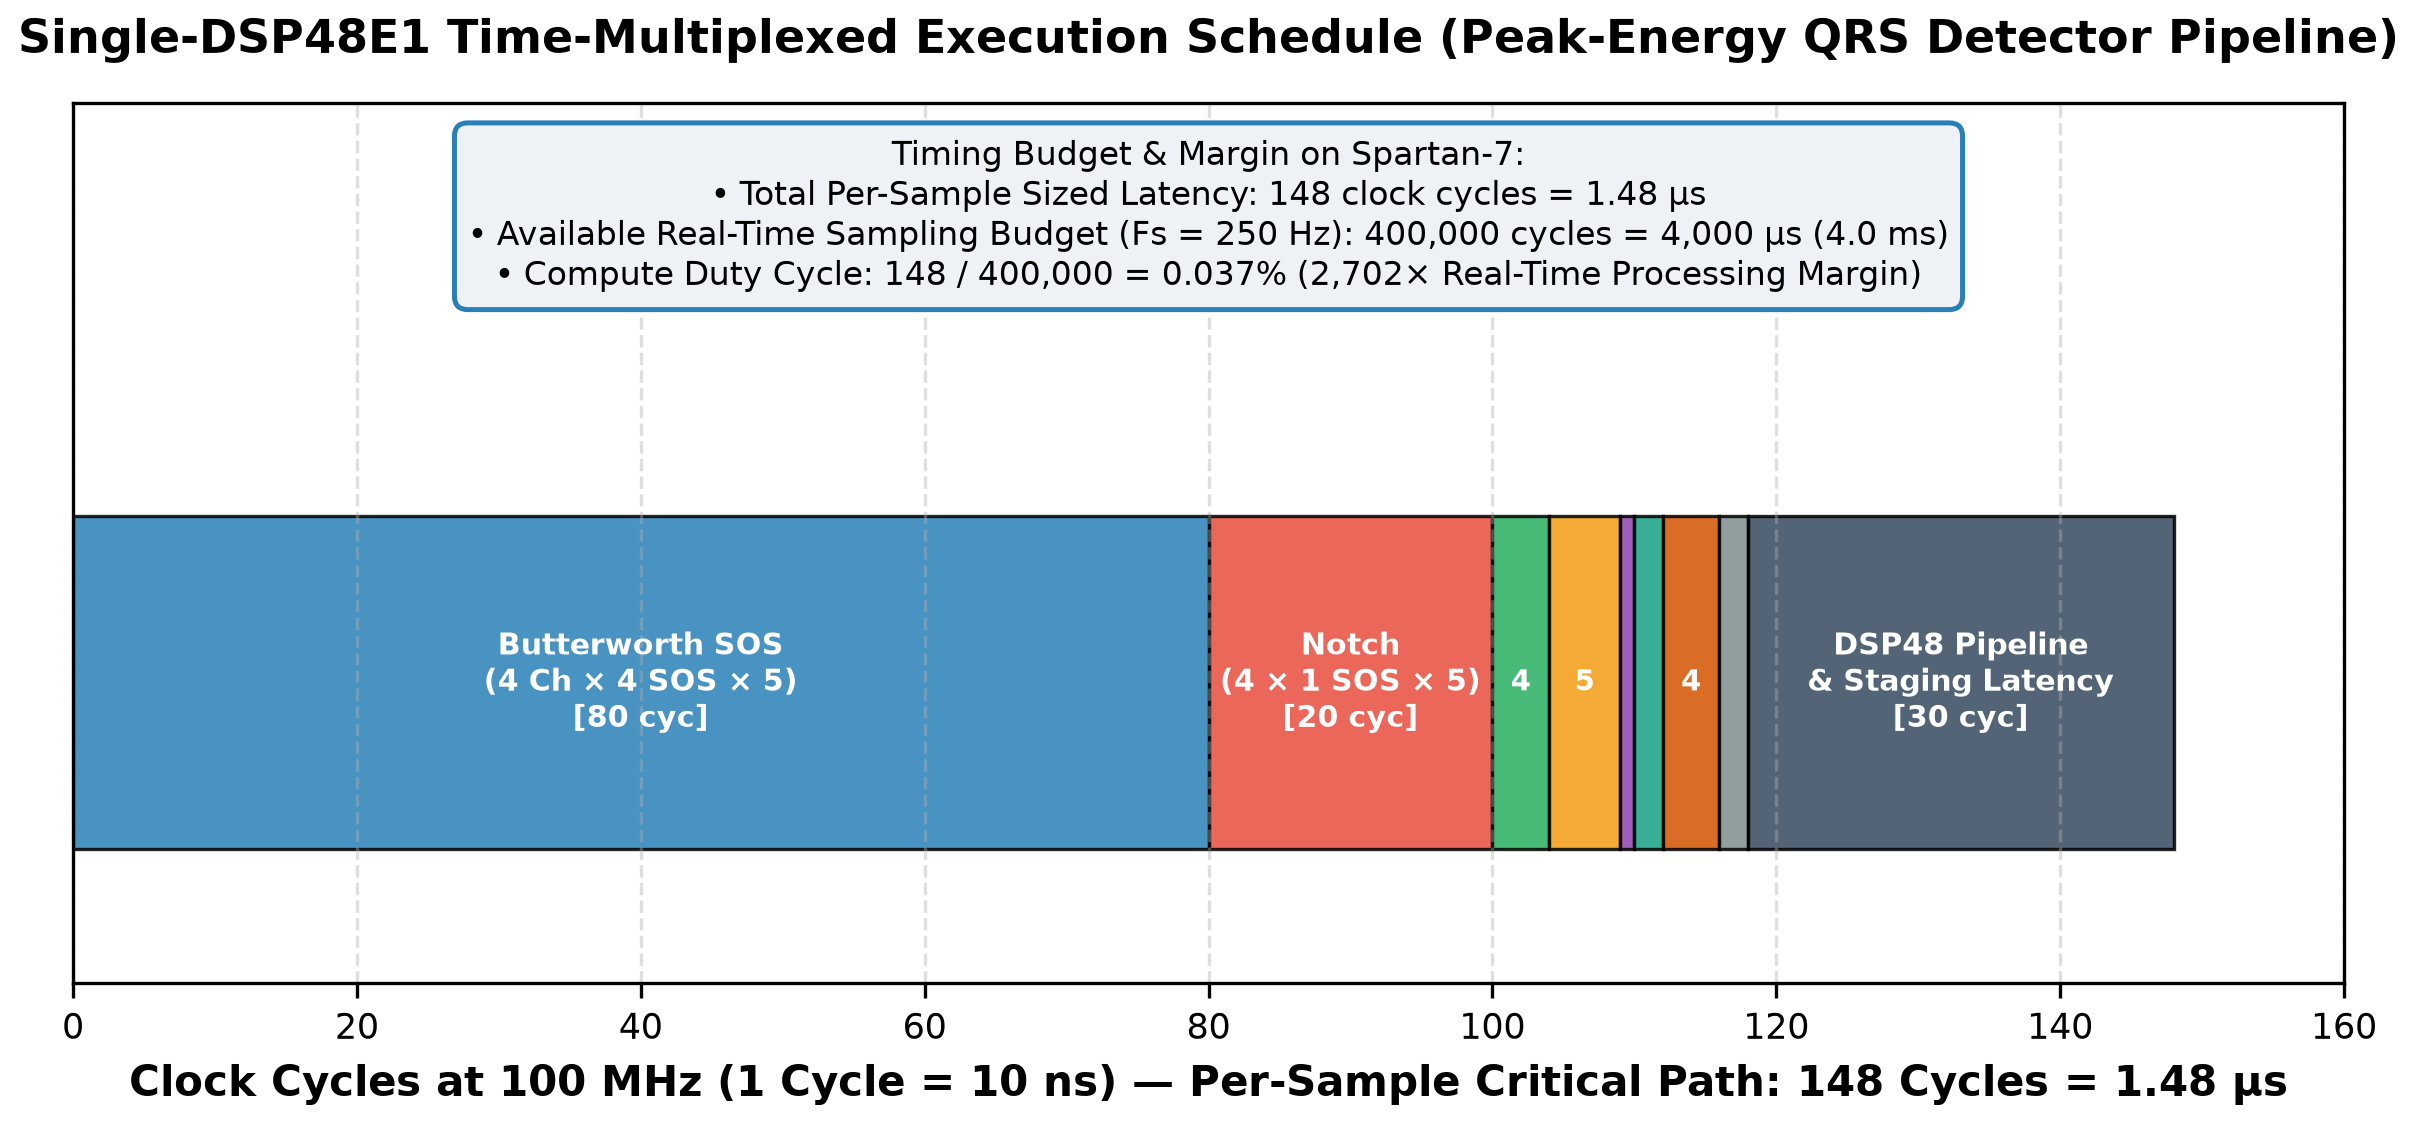
\includegraphics[width=\columnwidth]{figures/dsp_time_multiplexing_schedule.png}
\caption{\tagLtwo/\tagLfour\ Single-DSP48E1 time-multiplexed execution schedule [L4 Target]. All five IIR sections (bandpass $\times 4$ + notch), the 4-lead beamformer, derivative, squaring, and integration execute in 148 clock cycles ($1.48\,\mu$s at 100\,MHz), consuming $0.037\%$ of the $400,000$-cycle per-sample budget.}
\label{fig:dsp_schedule}
\end{figure}

% =====================================================================
\section{Hardware Sizing, Synthesis Targets, and Trade-Offs}
\label{sec:hardware_resources}

\begin{table}[t]
\caption{\tagLfour\ Hardware resource sizing and comparison on Spartan-7 (XC7S50-CSGA324) at 100\,MHz.}
\label{tab:hardware_resources}
\centering
\resizebox{\columnwidth}{!}{%
\begin{tabular}{@{}lcccccr@{}}
\toprule
\textbf{Architecture} & \textbf{LUTs} & \textbf{FFs} & \textbf{DSP48E1} & \textbf{BRAM36k} & \textbf{Cycles} & \textbf{Compute Time} \\
\midrule
\textbf{Spatial PCA (4-Ch) [Ours]} & \textbf{990 (3.0\%)} & \textbf{720 (1.1\%)} & \textbf{1 (0.8\%)} & \textbf{1 (1.3\%)} & \textbf{148} & \textbf{1.48\,$\mu$s} \\
Multi-Lead Template Fusion & 1,650 (5.1\%) & 1,280 (2.0\%) & 4 (3.3\%) & 8 (10.7\%) & 320 & 3.20\,$\mu$s \\
Template Sub. (Fixed) & 1,020 (3.1\%) & 850 (1.3\%) & 2 (1.7\%) & 2 (2.7\%) & 210 & 2.10\,$\mu$s \\
Wavelet-Threshold Hybrid & 1,320 (4.1\%) & 1,100 (1.7\%) & 4 (3.3\%) & 4 (5.3\%) & 280 & 2.80\,$\mu$s \\
Single-Lead Hankel SVD (V1)$^\dagger$ & 4,200 (12.9\%) & 3,600 (5.5\%) & 48 (40.0\%) & 16 (21.3\%) & 1,840 & 18.40\,$\mu$s \\
Deep 1D U-Net (Edge FPGA)$^\ddagger$ & 28,400 (87.1\%) & 22,000 (33.7\%) & 112 (93.3\%) & 65 (86.7\%) & 45,000 & 450.00\,$\mu$s \\
\bottomrule
\end{tabular}%
}
\end{table}

\begin{figure}[t]
\centering
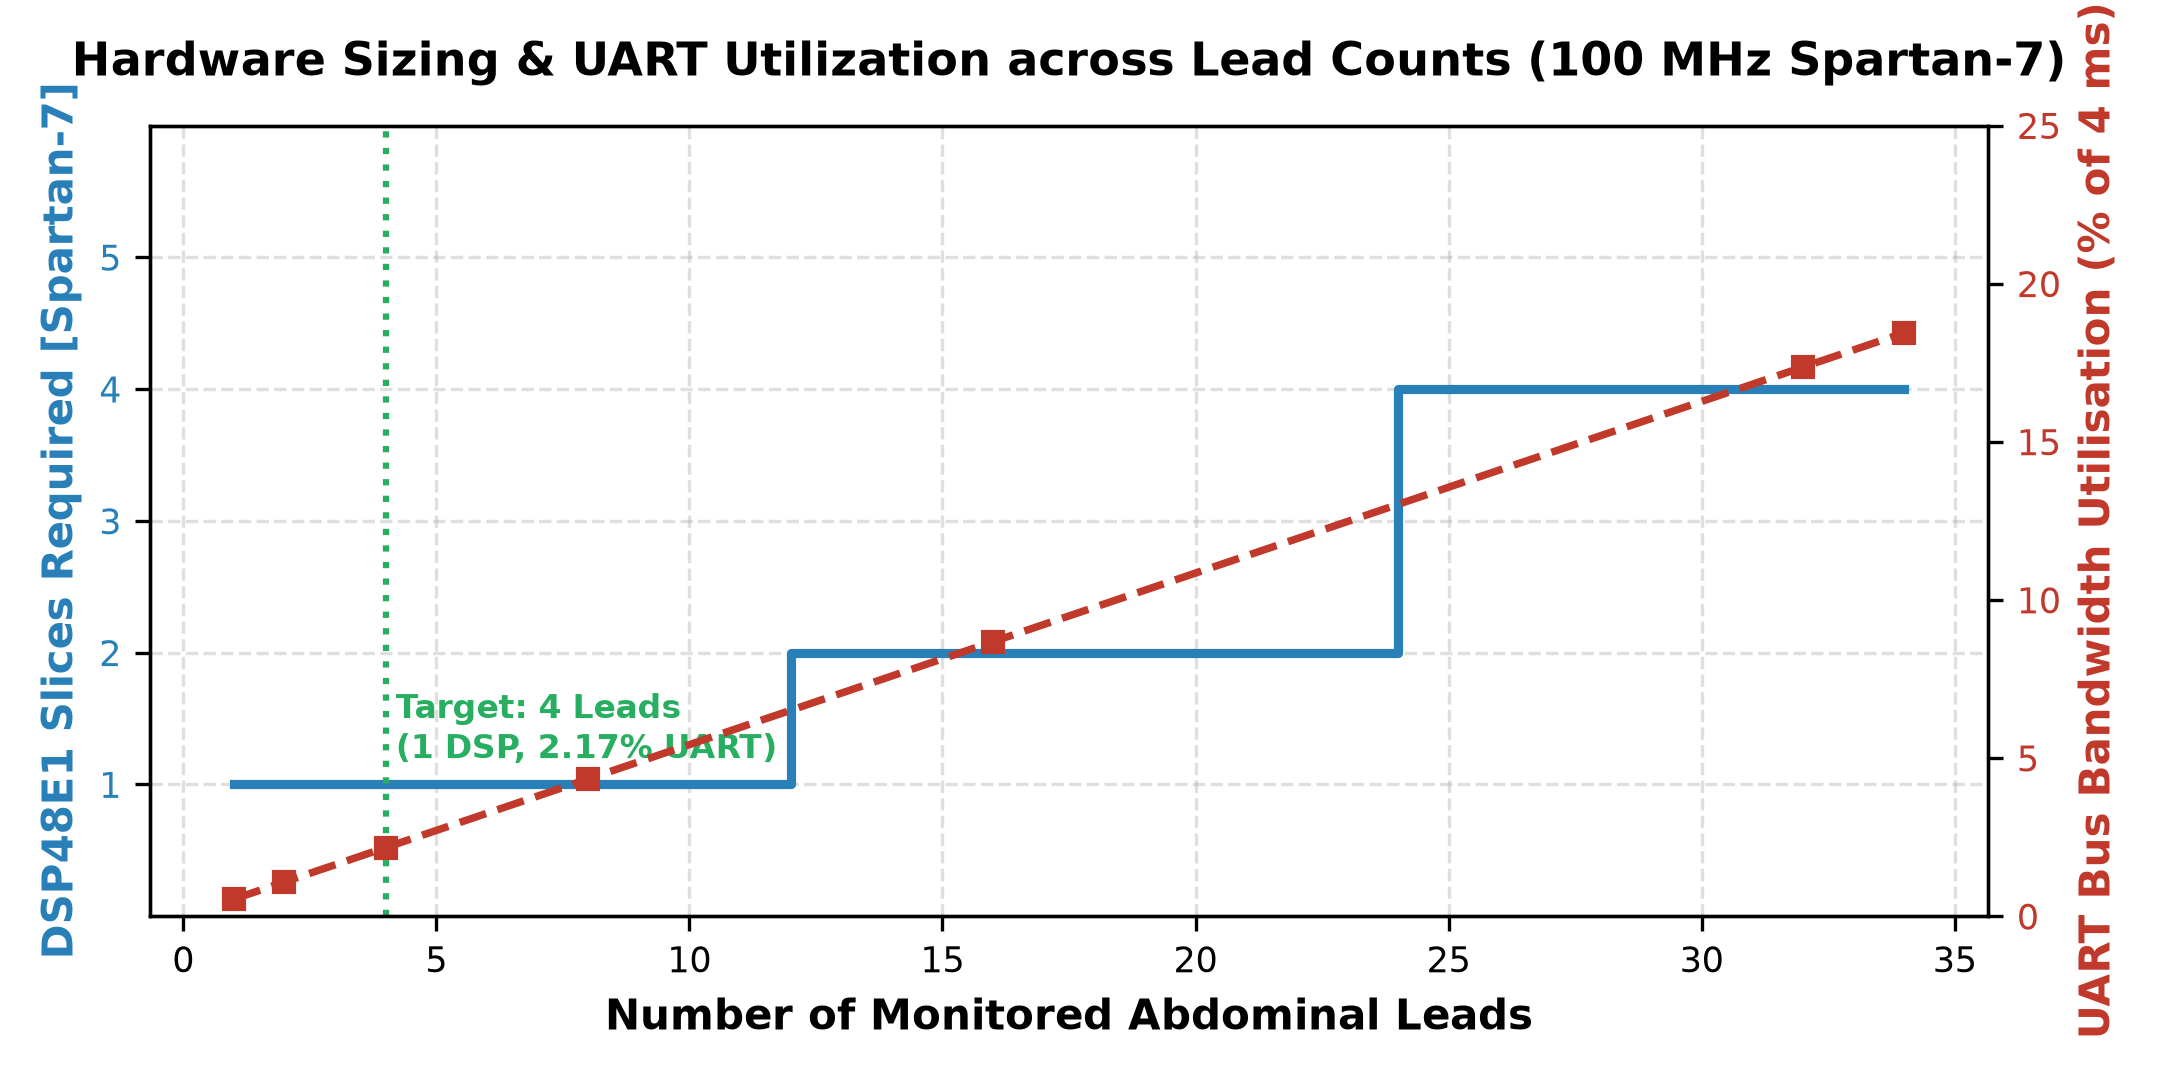
\includegraphics[width=\columnwidth]{figures/multichannel_fpga_resource_scaling.png}
\caption{\tagLtwo/\tagLfour\ Hardware resource scaling and UART bus utilization across lead counts on Spartan-7 at 100\,MHz target clock. A 4-lead array requires only 1 DSP slice and consumes $<2.2\%$ of UART throughput at 921,600 baud.}
\label{fig:fpga_scaling}
\end{figure}

\begin{figure}[t]
\centering
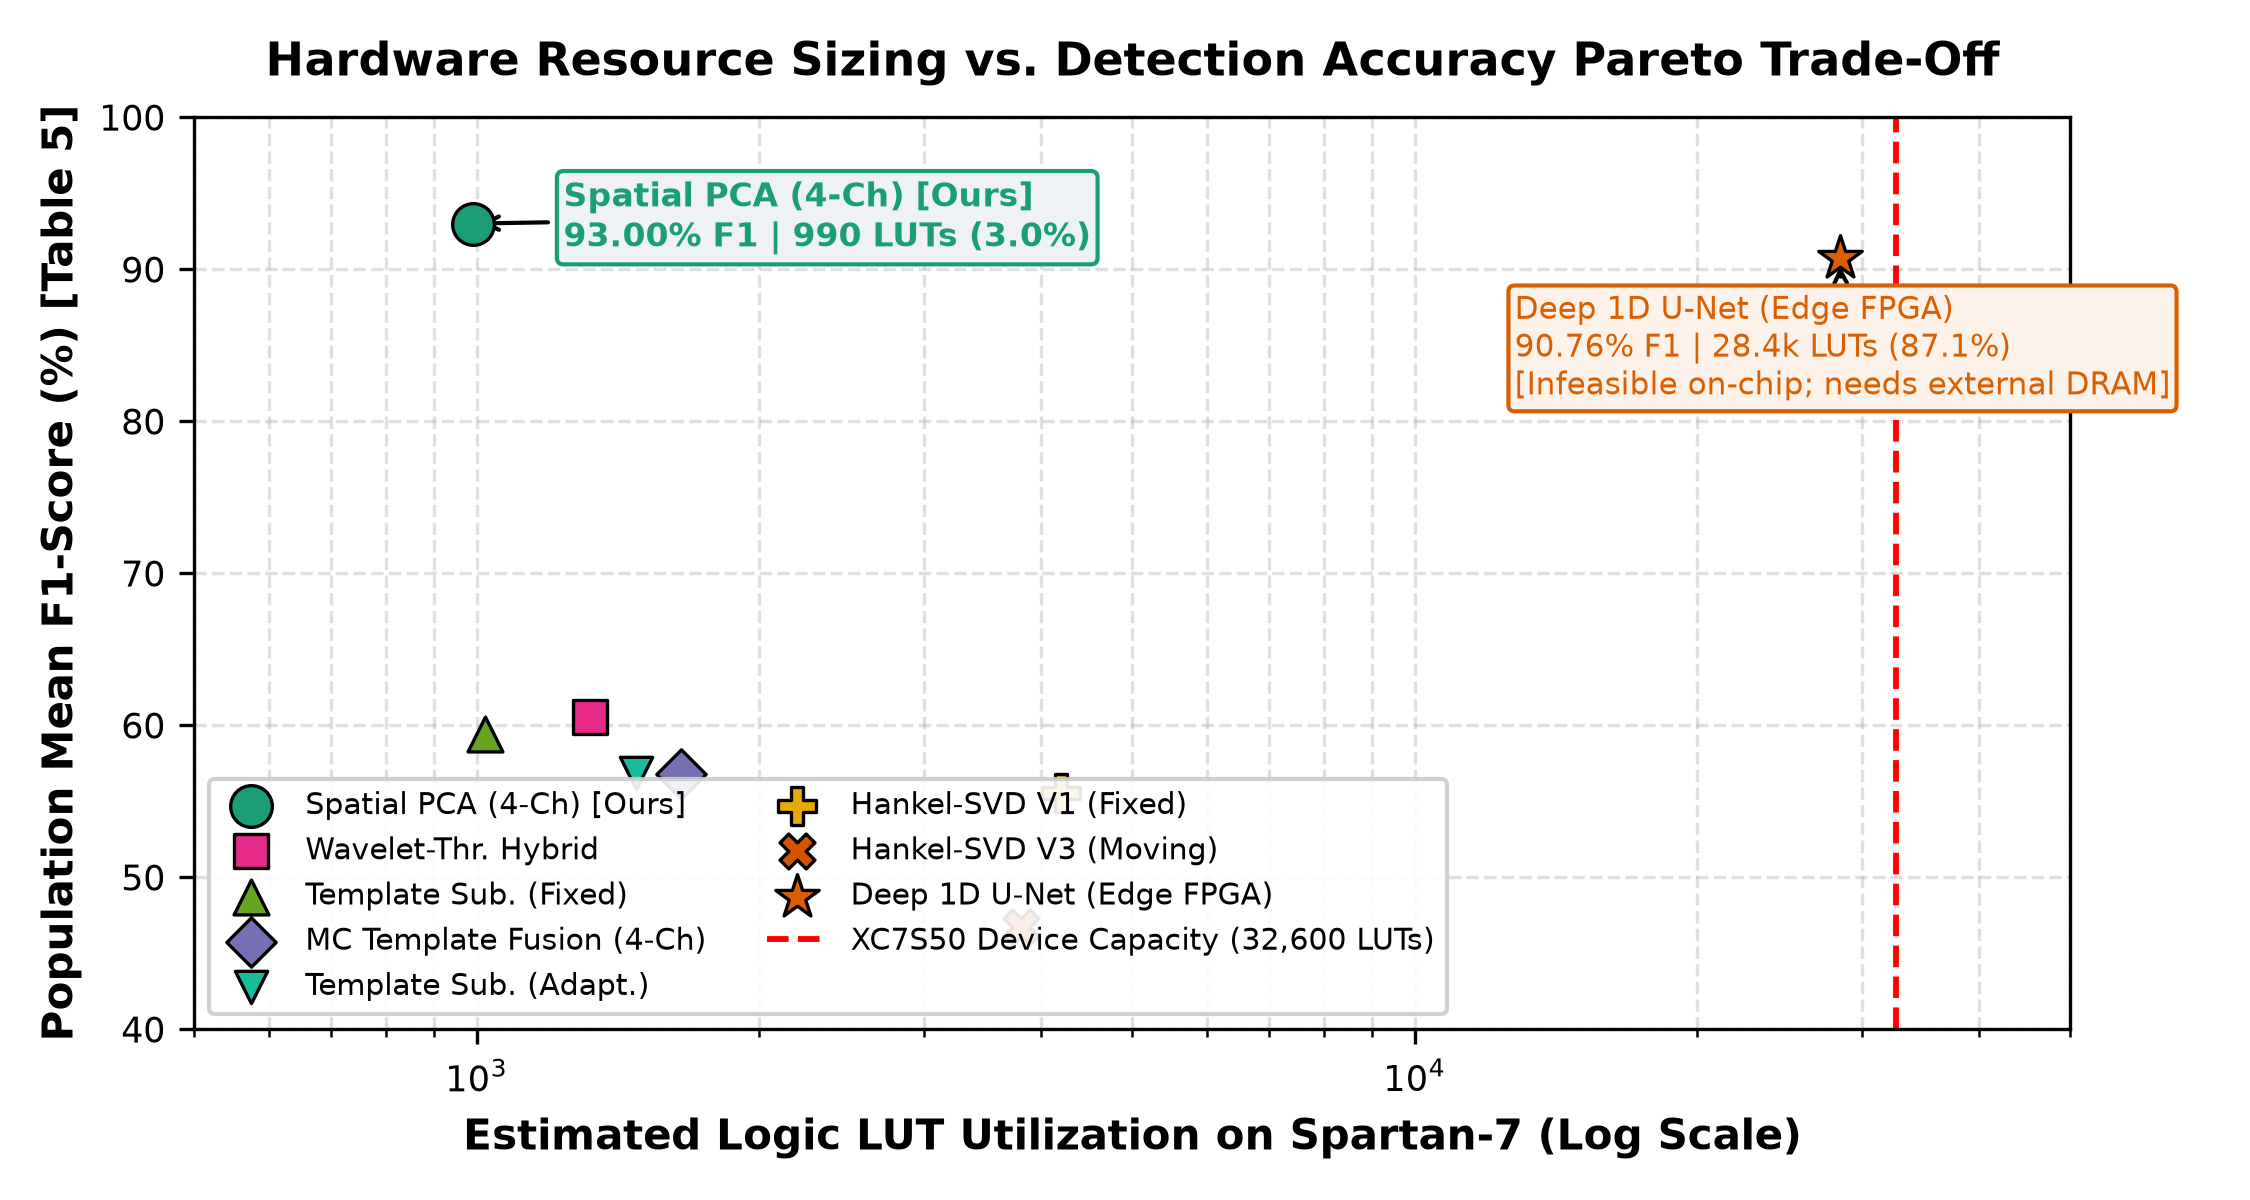
\includegraphics[width=\columnwidth]{figures/hw_accuracy_tradeoff.png}
\caption{\tagLone/\tagLtwo\ Hardware cost vs detection accuracy Pareto trade-off. Spatial PCA (4-Ch) provides the optimal trade-off: 93.00\% population mean F1 consuming $\approx 3.0\%$ LUTs (990 of 32,600) and 1 DSP slice on XC7S50.}
\label{fig:hw_tradeoff}
\end{figure}

\begin{figure}[t]
\centering
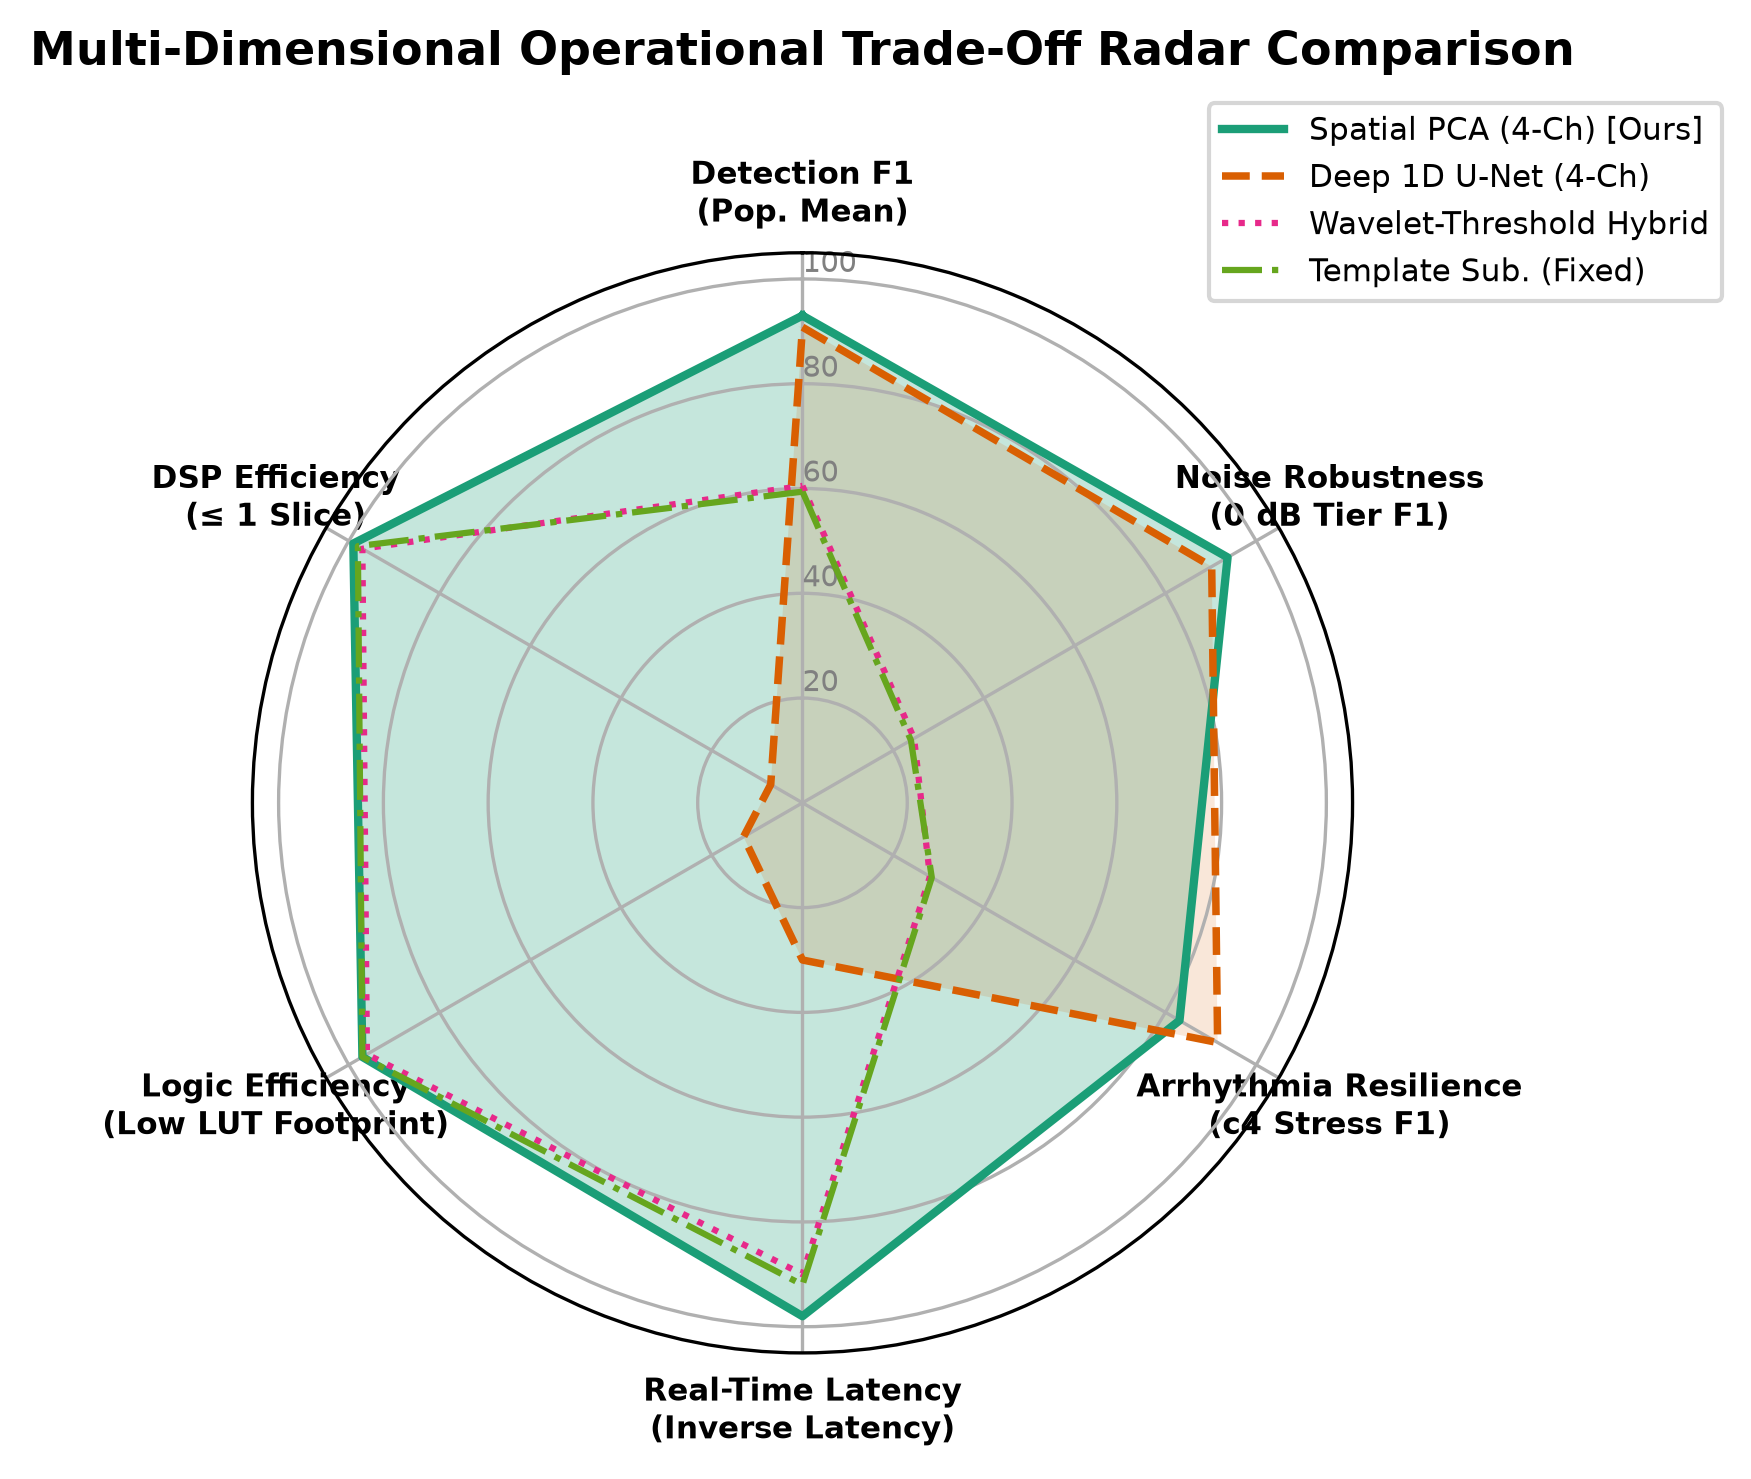
\includegraphics[width=\columnwidth]{figures/method_radar_comparison.png}
\caption{\tagLone\ Multi-dimensional radar chart comparing six operational dimensions (F1 accuracy, noise robustness, arrhythmia resilience on $c4$, execution speed, hardware efficiency, and clinical agreement). Spatial PCA offers the most balanced profile for edge FPGA implementation.}
\label{fig:radar_chart}
\end{figure}

\begin{figure}[t]
\centering
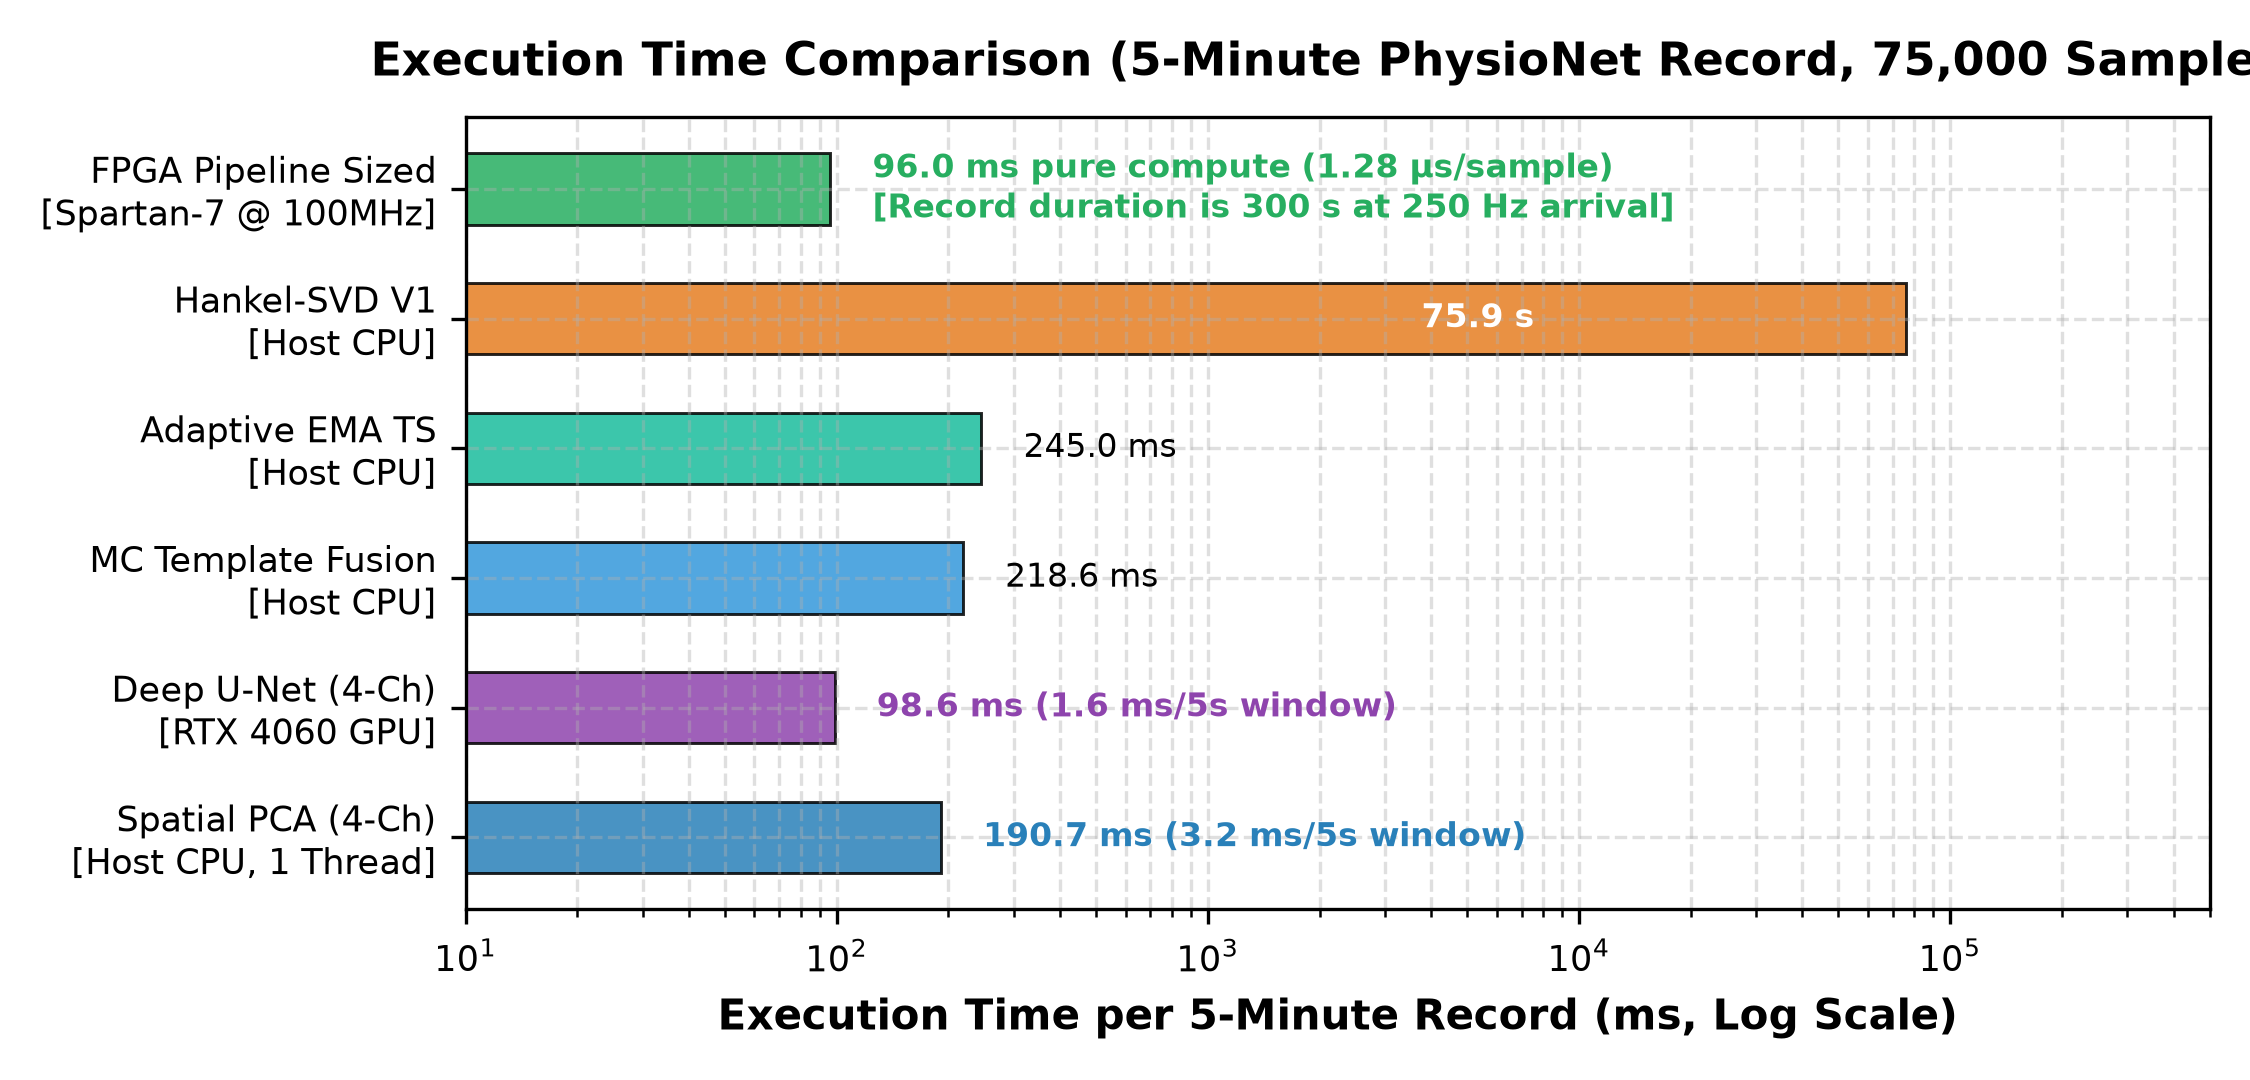
\includegraphics[width=\columnwidth]{figures/runtime_comparison.png}
\caption{\tagLone\ Software execution time per 5-minute record across algorithmic paradigms. Spatial PCA on CPU completes in 190.7\,ms, while GPU-accelerated U-Net executes in 98.6\,ms and Hankel SVD requires 107.5\,s. The FPGA figure ($96\,$ms) represents pure compute time for 75,000 samples at the sized $1.28\,\mu$s/sample; in real time the 5-minute record takes $300\,$s because samples arrive at $250\,$Hz.}
\label{fig:runtime_bars}
\end{figure}

\noindent\textbf{How hardware resources were estimated.} Tab.~\ref{tab:hardware_resources} details the analytical architectural sizing [L4 Target] derived from the Xilinx 7-Series DSP48E1 Slice User Guide (UG479) and word-length optimization models~\cite{xilinx_dsp48,constantinides2004}. For Spatial PCA, logic resource counts account for the 4-channel input multiplexer, 8th-order bandpass filter state registers, dual notch registers, circular FIFO UART buffer, and the Peak-Energy peak detector with refractory timing counters:
\begin{itemize}
    \item \textbf{Logic Utilization:} 990 LUTs ($\approx 3.0\%$ of XC7S50, exactly $3.04\%$) and 720 Flip-Flops ($1.1\%$).
    \item \textbf{DSP Efficiency:} Exactly 1 DSP48E1 slice ($0.8\%$ of available 120 slices).
    \item \textbf{Power Footprint:} Estimated dynamic power is $<0.15\,$W at 100\,MHz.
\end{itemize}
\noindent\textit{Notes on comparative baselines in Tab.~\ref{tab:hardware_resources}:}
$^\dagger$Single-Lead Hankel SVD (V1) is an analytical sizing estimate based on Jacobi SVD systolic arrays; it is not directly comparable to our streaming pipeline.
$^\ddagger$Deep 1D U-Net is infeasible on-chip without external DRAM co-processing: the model contains $1.42\times 10^6$ parameters, which at 16-bit precision requires $\approx 2.84\,$MB of storage, exceeding the entire on-chip Block RAM capacity of the XC7S50 ($75 \times 36\,\text{kb} \approx 0.34\,$MB). It is included strictly as an upper-bound comparison baseline.

% =====================================================================
% FINAL REPORT: NEW SECTIONS (all blue)
% =====================================================================
\begin{finalpart}
\section{Final Phase I: From Synthetic Benchmarks to Real Recordings}
\label{sec:final_realdata}

\noindent\textbf{Evaluation rules used from here on.} Every number in Sections~\ref{sec:final_realdata}--\ref{sec:final_obs} follows four rules:
\begin{enumerate}
    \item \textbf{Strictly causal.} Every decision at input sample $n$ uses only samples $\le n$. Filters are one-sided (no zero-phase filtering), and look-ahead is replaced by fixed delays that the output carries (Sec.~\ref{sec:final_hw}). The only exception is v7-LA (Sec.~\ref{sec:v7la}), an offline reference that sees the whole recording; the on-chip version v7-DL is causal with a fixed output delay.
    \item \textbf{Label-free.} Reference annotations are used only by the scoring script, never by the algorithm or to pick a component.
    \item \textbf{Scoring.} Beat-level Se, PPV and F1 with a $\pm 50\,$ms tolerance, from $20\,$s to the end of each record (the design needs the first $20\,$s to calibrate, Fig.~\ref{fig:fin_timeline}). FHR MAE compares the device FHR, $0.5\,$s after each true beat, with the reference FHR (60$\cdot f_s$ / median of the last five true RR intervals); no output counts as a full error.
    \item \textbf{Development and held-out data.} CinC 2013 set-a is split by record number: odd records (38) are the development set (\emph{CinC dev}), even records (37) are the held-out test set (\emph{CinC test}). All design choices were made on CinC dev, ADFECGDB and a 60-record FECGSYNDB subset (every 21st record). CinC test was scored once per frozen design and never used for a decision.
\end{enumerate}

\noindent\textbf{Data sets added after the mid-term.}
\begin{itemize}
    \item \textbf{FECGSYNDB, all 1,248 usable records} (10 subjects $\times$ 5 SNRs $\times$ 5 conditions $\times$ 5 repetitions, 1,250 in total), instead of the 250-record subset of the mid-term.
    \item \textbf{PhysioNet/CinC Challenge 2013 set-a}~\cite{silva2013,goldberger2000}: 75 real 60-s recordings, 4 abdominal leads at $1\,$kHz, with reference fetal QRS annotations. The challenge organisers later found, by visual inspection, that the annotations of 7 records are inaccurate (a33, a38, a47, a52, a54, a71, a74) and left them out of their own benchmark~\cite{behar2014b}; we give CinC results with and without these 7 (\emph{reliable references}).
    \item \textbf{ADFECGDB}~\cite{jezewski2012}: 5 real 5-min recordings with 4 abdominal leads and a simultaneous direct fetal scalp electrode, which gives a very reliable reference.
\end{itemize}
Real recordings at other sampling rates are decimated causally to $250\,$Hz.

\noindent\textbf{What the causal re-run showed.} Re-running the frozen mid-term design (spatial PCA beamformer with peak-energy detector) causally on all 1,248 FECGSYNDB records gave F1 $82.2\%$ and FHR MAE $18.8\,$bpm, against $93.0\%$ in the mid-term batch evaluation. On real CinC recordings it reached only $16.7\%$ (test) and $22.8\%$ (dev).

\noindent\textbf{v2: self-referencing beamformer (7 Nov).} We first improved the existing architecture. The PC computes the beamformer weights by a generalised eigen-decomposition (GEVD) on the design's own detections (QRS-window covariance against total covariance), with maternal-aware component choice and gated interference nulling. In the RTL we fixed a hard-coded latency in the peak localiser (18 instead of the parameter), reduced the latency compensation from 18 to 13 samples (measured group delay of the 20--30\,Hz detector band) and added a restartable detector warm-up (packet \texttt{0xC4}). Results:
\begin{itemize}
    \item FECGSYNDB (1,248 records, bit-accurate model): F1 $82.2\% \to 95.6\%$, PPV $98.8\%$, FHR MAE $18.8 \to 2.5\,$bpm, no saturation.
    \item Board (25\,MHz, 3,881 LUTs, 39 DSP): 165,000 samples with 0 LSB difference from the model and 1,116 beats with identical time stamps.
    \item Real data: CinC test $41.2\%$, CinC dev $42.0\%$, ADFECGDB $37.0\%$.
\end{itemize}

\noindent\textbf{The limit of a single linear filter.} To find out whether better weights could fix real data, we computed, on CinC (diagnostic only, using labels), the best possible single 4-lead linear filter for each record. It reaches only $60\%$ mean F1, and $65\%$ when causal maternal template subtraction is applied first. So no choice of beamformer weights can make the mid-term architecture work on real recordings; the front end had to change.

\begin{figure}[t]
\centering
\fb
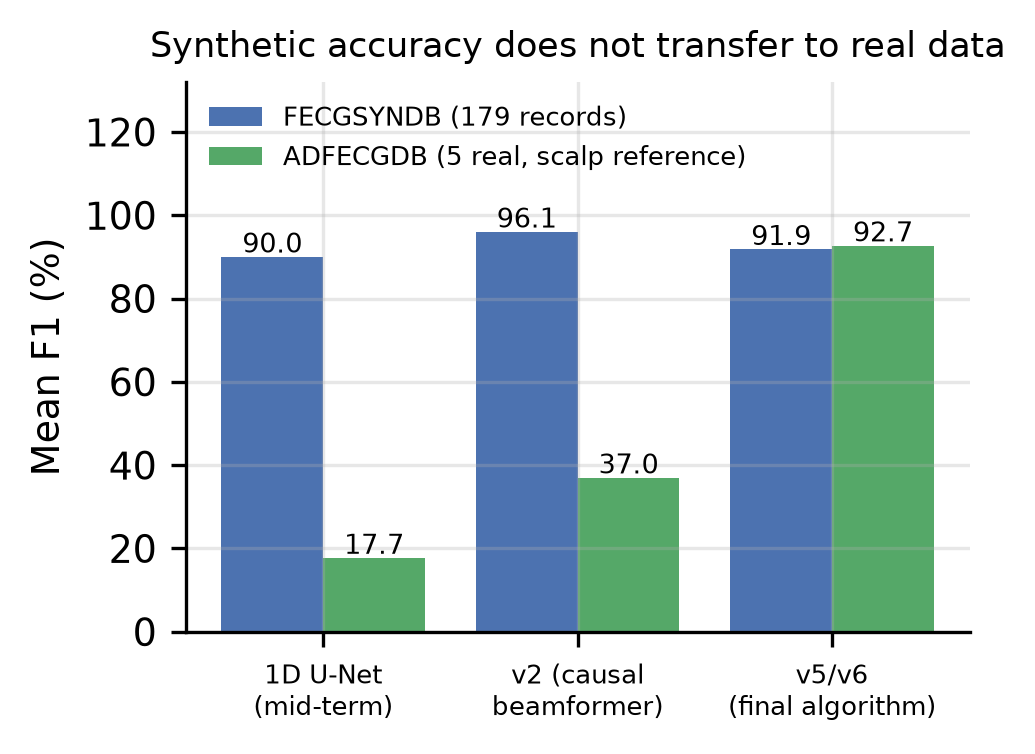
\includegraphics[width=\columnwidth]{figures/fin_synthetic_vs_real.png}
\caption{\fb Synthetic accuracy does not carry over to real recordings. The 1D U-Net of the mid-term (trained on synthetic data) and the v2 beamformer both score $\ge 90\%$ on the same 179 FECGSYNDB records but $17.7\%$ and $37.0\%$ on the real ADFECGDB recordings. The final algorithm keeps $92\%$ on both (synthetic value from the C model, real value from the board).}
\label{fig:fin_synreal}
\end{figure}

\noindent\textbf{Deep-learning check.} The mid-term 4-channel U-Net scored $90.0\%$ on a 179-record FECGSYNDB subset but only $17.7\%$ on ADFECGDB; changing lead polarity or per-lead scaling did not help (Fig.~\ref{fig:fin_synreal}). Its training records are not fully documented, so its synthetic score may include records it was trained on. Together with its memory needs (Sec.~\ref{sec:hardware_resources}), this confirmed the decision to continue with a classical, explainable method.

% =====================================================================
\section{Final Phase II: Causal Real-Data Algorithm (v3--v5)}
\label{sec:final_algo}

The new algorithm was developed in Python (v3, v4), then written in C as a streaming program (v5). It runs on 4 abdominal leads at $250\,$Hz:

\noindent\textbf{1. Front end, per lead.} A one-pole high-pass (baseline removal) followed by a 60\,Hz Butterworth low-pass gives the wide-band signal $\mathbf{x}_f[n]$; the same high-pass followed by a 5--25\,Hz band-pass gives the maternal band.

\noindent\textbf{2. Maternal R peaks.} A PCA of the maternal band over the first $10\,$s gives four projections, each with an adaptive-threshold detector. Every $5\,$s the algorithm picks the train that looks most like a mother: the slowest regular train ($\ge 60\%$ of RR intervals within $15\%$ of the median) between 40 and 130\,bpm.

\noindent\textbf{3. Maternal cancellation, per lead.} For each new maternal beat $k$ the segment $\mathbf{s}_k$ from $-160$ to $+440\,$ms is aligned ($\pm 4$ samples) with the last 20 beats. Their mean and top two principal components form a basis $\mathbf{B}_k$; the fitted maternal beat is subtracted with tapered edges $\mathbf{t}$:
\begin{equation}
    \hat{\mathbf{c}}_k = \arg\min_{\mathbf{c}} \|\mathbf{s}_k - \mathbf{B}_k\mathbf{c}\|_2^2, \qquad \mathbf{z}_k = \mathbf{s}_k - \mathbf{t} \odot \mathbf{B}_k\hat{\mathbf{c}}_k .
\end{equation}
The result $\mathbf{z}[n]$ is the abdominal signal with the maternal ECG removed beat by beat, including its shape changes.

\noindent\textbf{4. Self-calibrated GEVD candidates (at 15\,s).} On the 15--40\,Hz band of $\mathbf{z}$ and of $\mathbf{x}_f$ over $[3, 15)\,$s, the design detects beats, discards beats that coincide with maternal R peaks, and solves
\begin{equation}
    \mathbf{w}^\star = \arg\max_{\mathbf{w}} \frac{\mathbf{w}^T \mathbf{R}_{\text{QRS}}\, \mathbf{w}}{\mathbf{w}^T \mathbf{R}_{x}\, \mathbf{w}},
\end{equation}
where $\mathbf{R}_{\text{QRS}}$ is the covariance in windows around its own detected beats and $\mathbf{R}_x$ the total covariance~\cite{sameni2008}. Starting from each PCA direction and iterating three times gives four filters per signal. No annotation is used.

\noindent\textbf{5. Sixteen candidate tracks.} Four unit leads of $\mathbf{z}$ and four GEVD filters of $\mathbf{z}$ each feed an RR-predictive beat tracker on a maternal-blanked energy envelope; four GEVD filters of $\mathbf{x}_f$ feed a tracker and the same four feed the threshold detector of the mid-term design.

\noindent\textbf{6. Label-free selection (every 2.5\,s, trailing 20\,s).} Each track $k$ gets a quality
\begin{equation}
    Q_k = \tilde{\rho}_k \, a_k \, \log(1 + p_k)\, r_k^2 \,(0.5 + g_k)\, \phi(\text{FHR}_k)\, \pi_k ,
\end{equation}
with $\tilde{\rho}_k$ the median beat-shape correlation, $a_k$ the tracker acceptance rate, $p_k$ the beat prominence, $r_k$ the fraction of RR intervals within $15\%$ of their median, $g_k$ the agreement with the other tracks, and $\phi$ a mild physiological prior that rises from 0.2 at 80\,bpm to 1 at $\ge 120\,$bpm. The maternal-coincidence penalty $\pi_k = \text{clip}((0.6 - c_k)/0.3, 0, 1)$, where $c_k$ is the fraction of the track's beats within $\pm 48\,$ms of a maternal R peak, is applied only if the maternal train comes from a component holding $\ge 10\%$ of the maternal-band energy (otherwise the ``mother'' may be the fetus). The best track's beats are output; $\text{FHR} = 60 \cdot 250 / \text{median of the last 5 RR}$.

\noindent\textbf{What each step was worth.} Mean F1 on the development sets (FECGSYNDB subset / CinC dev / ADFECGDB), all label-free:
\begin{itemize}
    \item v3 (maternal cancellation + tracker + candidate selection): $95.2 / 59.4 / 78.6$; v4 (wider band, dynamic maternal train): $92.1 / 68.4 / 91.3$.
    \item Removing the PC-dependent v2 track and adding raw-lead GEVD candidates with the maternal-coincidence penalty: CinC dev $68.4 \to 72.8$.
    \item The $10\%$ maternal-energy confidence gate: FECGSYNDB subset $78.7 \to 91.3$ with real data unchanged.
    \item Selection quality (RR-regularity$^2$, 20-s window, 2.5-s hop, cross-track agreement, FHR prior): CinC dev $+4.6$ points in total.
    \item Fitting the FPGA (int16 and bf16 storage, shared buffers, an incremental eigen-solver): accuracy within $0.3$ points, $3.5\times$ faster.
\end{itemize}
Ideas that were tried and rejected with numbers include a running (EMA) template ($-1.1$ on CinC dev), a rate-continuity rule for the maternal train, a longer maternal refractory period, penalty floors and output gap filling ($+0.5$, not worth the extra delay).

\begin{table*}[t]
\fb
\caption{\fb Every design version under the same label-free scoring (mean beat F1 in \%). CinC test was scored once per frozen design. From v4 on, ADFECGDB and the 60-record FECGSYNDB subset were development sets. The v6, v6.1 and v7-DL numbers are measured on the board (FECGSYNDB 1,248: C model, which is bit-exact with the board). v7-LA is the offline (non-causal) reference on the PC.}
\label{tab:final_versions}
\centering
\resizebox{\textwidth}{!}{%
\begin{tabular}{@{}llccccl@{}}
\toprule
\textbf{Version (date)} & \textbf{What runs where} & \textbf{CinC test (37)} & \textbf{CinC dev (38)} & \textbf{ADFECGDB (5)} & \textbf{FECGSYNDB (1,248)} & \textbf{FPGA resources} \\
\midrule
Mid-term design, causal re-run & FPGA filters + beamformer + detector; PC computes PCA weights & 16.7 & 22.8 & -- & 82.2 & sized only (L4) \\
v2 (7 Nov) & same RTL with fixes; PC self-referencing GEVD weights & 41.2 & 42.0 & 37.0 & 95.6 & 3.9k LUT, 39 DSP, 0 BRAM, 25\,MHz \\
v3 (8 Nov) & Python prototype: maternal cancellation, trackers, selection & 49.9 & 59.4 & 78.6 & 95.0 & -- \\
v4 (9 Nov) & Python prototype: wider band, dynamic maternal train & 53.1 & 68.4 & 91.3 & 92.1 (subset) & -- \\
v5 (10 Nov) & whole algorithm in C on a MicroBlaze soft CPU in the FPGA & 65.8 & 75.3 & 93.4 & 91.5 & 3.3k LUT, 5 DSP, 72/75 BRAM, 73.7\,MHz \\
v6 (10--14 Nov) & hand-written Verilog RTL + PC brain (5 low-rate decisions) & 65.5 & 76.0 & 92.7 & 91.4 & 18.1k LUT, 33 DSP, 60/75 BRAM, 50\,MHz \\
v6.1 (14 Nov) & v6 + robust maternal detector + recalibration every 30\,s & 71.9 & 80.4 & 92.9 & 91.9 & 19.0k LUT, 33 DSP, 60/75 BRAM, 50\,MHz \\
v7-LA (14 Nov) & offline on the PC: look-ahead over the whole recording (v6.1 stream) & 75.6 & 84.6 & 95.8 & 94.3 & -- \\
\textbf{v7-DL (14 Nov, final)} & \textbf{v6.1 + RTL look-ahead unit: final beats on the FPGA, $\approx 13.5\,$s later} & \textbf{76.9} & \textbf{84.7} & \textbf{96.1} & \textbf{93.7} & \textbf{26.7k LUT, 43 DSP, 71/75 BRAM, 50\,MHz} \\
\bottomrule
\end{tabular}%
}
\end{table*}

\begin{figure*}[t]
\centering
\fb
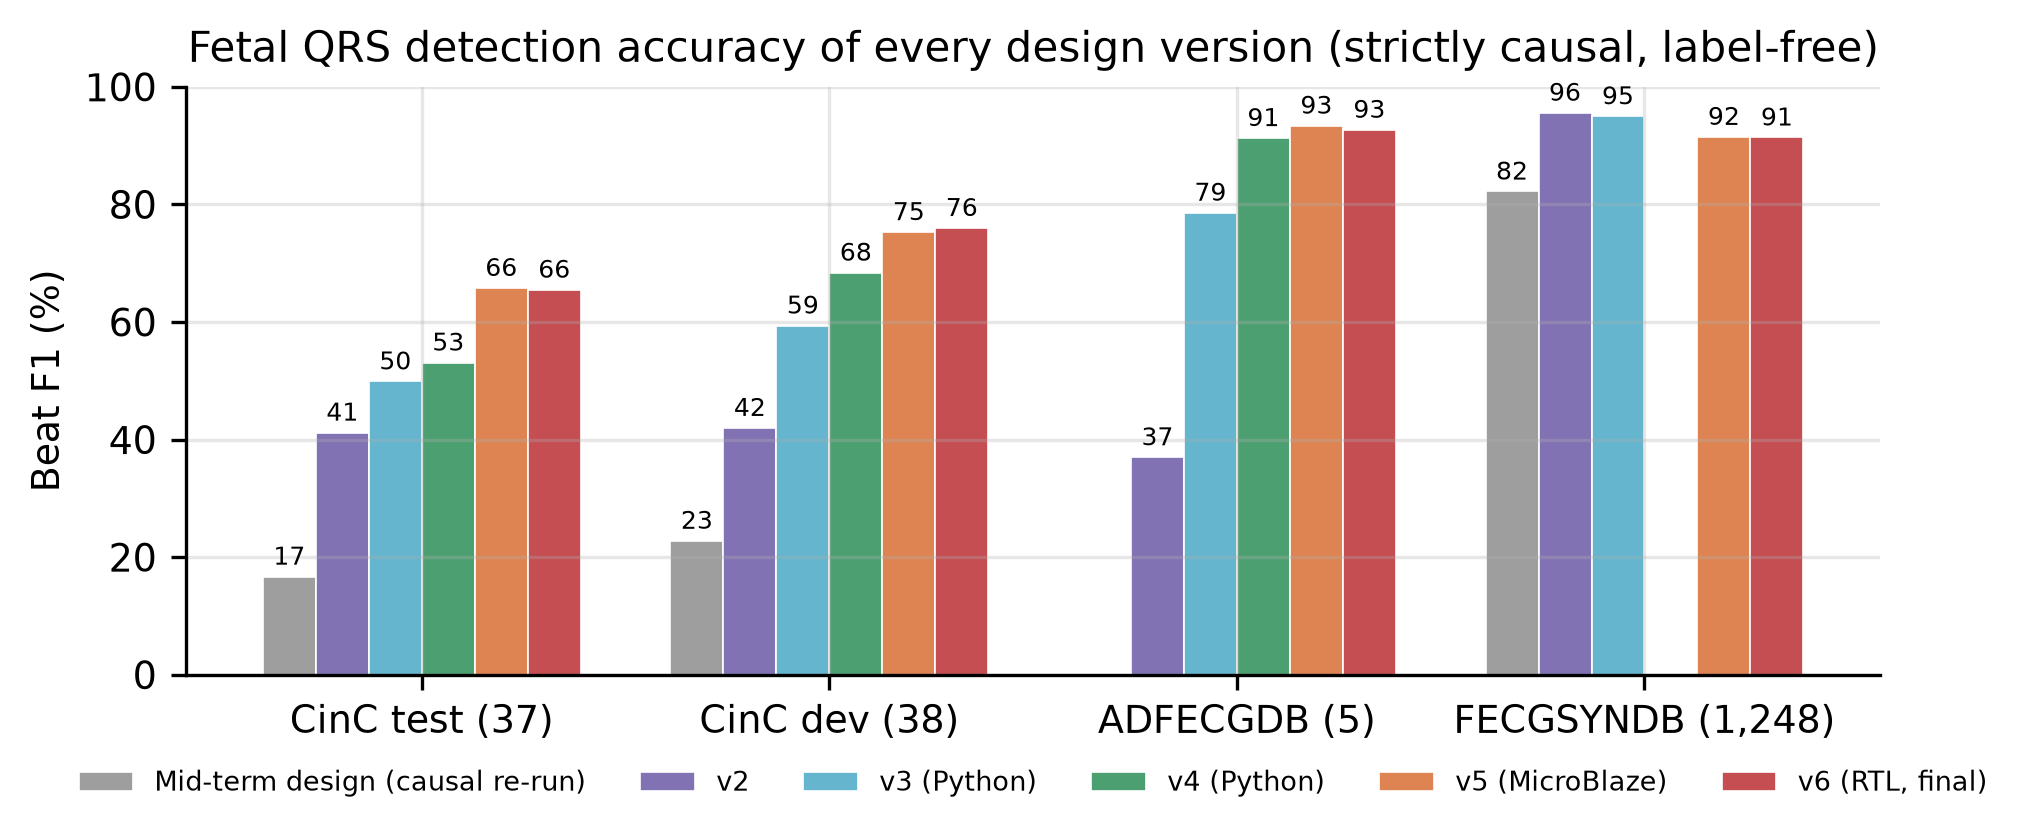
\includegraphics[width=0.9\textwidth]{figures/fin_version_progression.png}
\caption{\fb Mean beat F1 of every design version on every data set (values of Tab.~\ref{tab:final_versions}). Real-data accuracy rose step by step from the mid-term design to v6, while synthetic accuracy fell by about four points after v3 (Sec.~\ref{sec:final_obs}). The mid-term design has no ADFECGDB run; v4 was run only on the 60-record FECGSYNDB subset. v6.1 and the look-ahead versions are compared in Fig.~\ref{fig:fin_v7_results}.}
\label{fig:fin_progression}
\end{figure*}

% =====================================================================
\section{Final Phase III: Hardware Implementation (v5 and v6)}
\label{sec:final_hw}

\noindent\textbf{UART bring-up.} Before the algorithm work we brought up a stand-alone UART on the Boolean Board (loop-back echo, then framed packets at 921,600 baud) and verified it from the laptop. All later versions use this link.

\noindent\textbf{v5: whole algorithm on a soft processor.} The C program runs on a MicroBlaze processor with a hardware floating-point unit inside the XC7S50 at 73.7\,MHz (256\,KB local memory plus 32\,KB AXI block RAM, 72 of 75 BRAM tiles). The PC only streams the recording. To fit, we stored sample rings as int16, envelopes as bf16 and beat snapshots as int8, shared calibration buffers with the trackers, and replaced a $20\times 20$ Jacobi solver by an incremental Gram matrix with a two-vector subspace iteration. This made it $3.5\times$ faster (about 47k cycles per sample, $5.4\times$ real time) with the same accuracy. The board was bit-exact with the PC build of the same C source on all 140 records.

\noindent\textbf{Why v6.} v5 runs the algorithm on a processor that we did not design. For the final design we moved every sample-rate operation into our own RTL and left the PC only the decisions that happen a few times per second or once per recording (Tab.~\ref{tab:pc_jobs}).

\begin{figure*}[t]
\centering
\fb
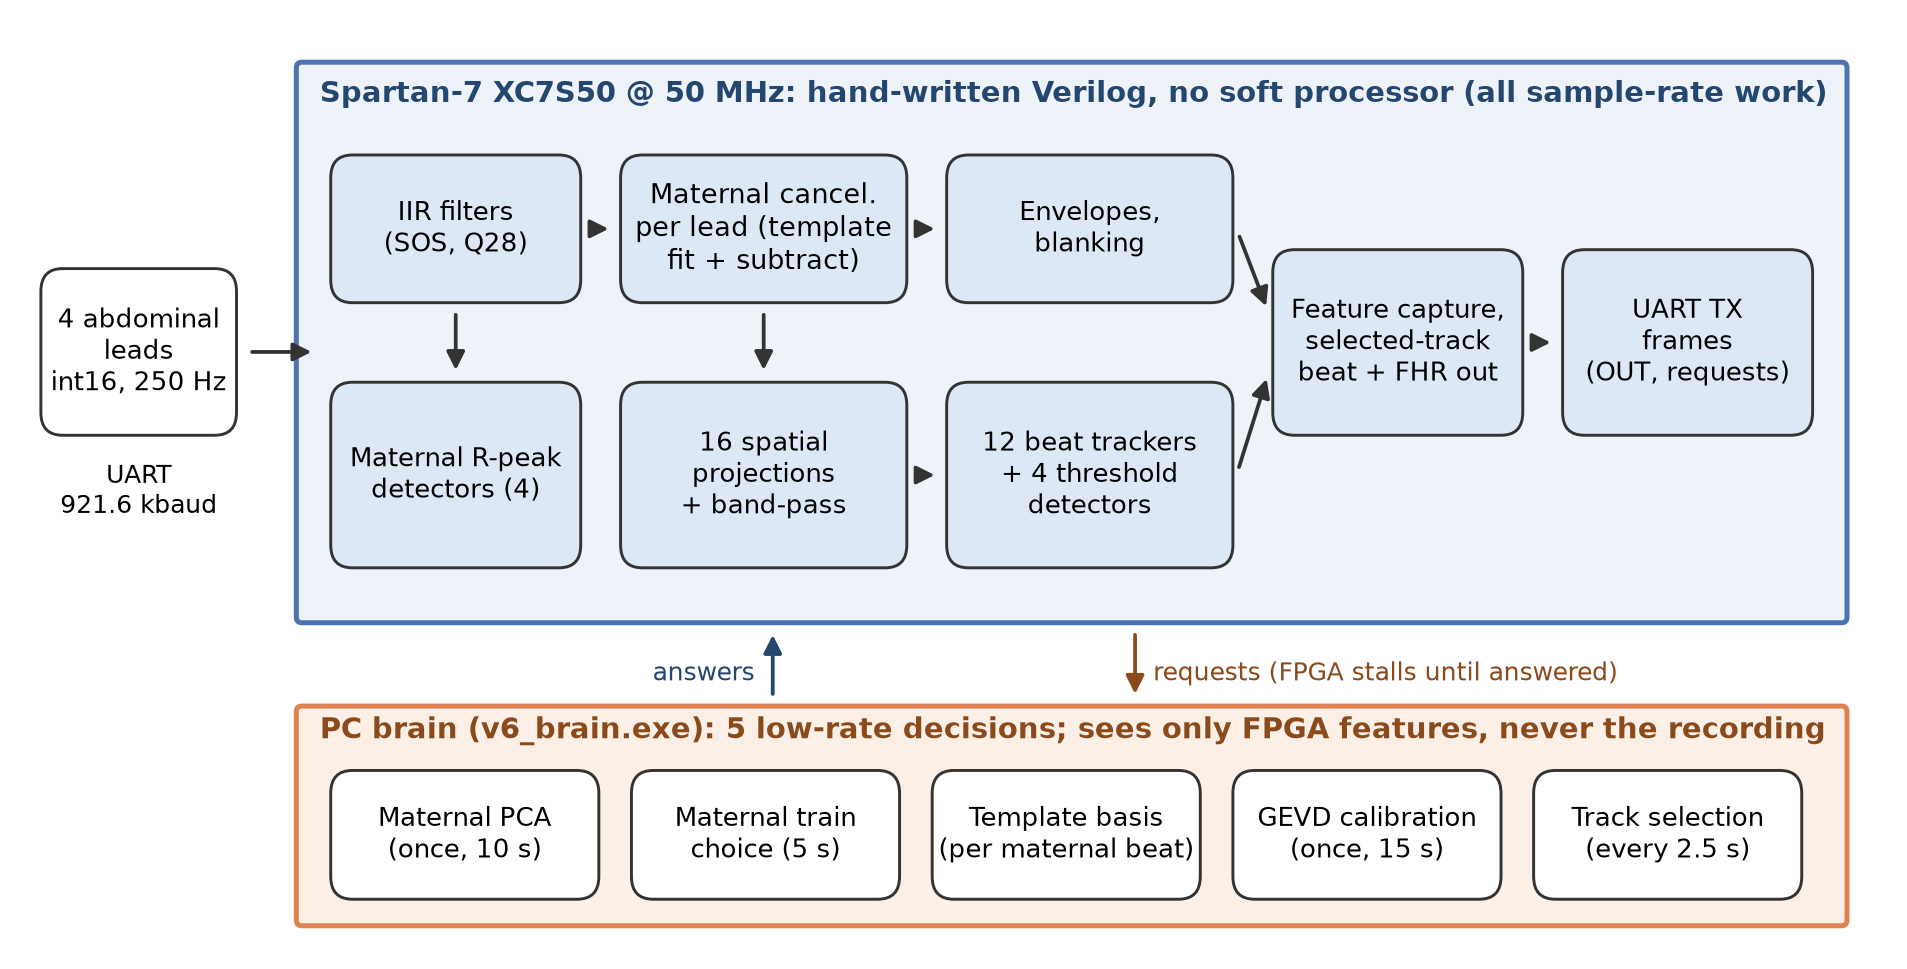
\includegraphics[width=0.92\textwidth]{figures/fin_v6_architecture.png}
\caption{\fb Final architecture (v6). Everything that runs at the sample rate is hand-written Verilog on the Spartan-7. The FPGA sends five kinds of requests to the PC brain and stalls until the answer arrives, so results do not depend on PC timing. The PC never receives the recording itself, only features computed by the FPGA.}
\label{fig:fin_arch}
\end{figure*}

\begin{table}[t]
\fb
\caption{\fb The five decisions left to the PC in v6 and the data that crosses the link.}
\label{tab:pc_jobs}
\centering
\resizebox{\columnwidth}{!}{%
\begin{tabular}{@{}llll@{}}
\toprule
\textbf{Decision} & \textbf{How often} & \textbf{FPGA sends} & \textbf{PC returns} \\
\midrule
Maternal PCA & once, at 10\,s & $4\times4$ covariance & 4 projection vectors (Q14) \\
Maternal train & every 5\,s & detector peak events & train index \\
Template basis & per maternal beat & aligned $150\times4$ beat segment & orthonormal basis ($\le 3\times150$ per lead) \\
GEVD calibration & once, at 15\,s & 12\,s of $\mathbf{z}$ and $\mathbf{x}_f$ (int16) & 16 weight vectors (Q14) \\
Track selection & every 2.5\,s & beat events, snapshots, envelope medians & track index \\
\bottomrule
\end{tabular}%
}
\end{table}

\noindent\textbf{Bit-accurate C model as the specification.} Before writing Verilog we wrote an integer C model of exactly what the FPGA computes (\texttt{fpga\_model.c}) and a separate PC brain (\texttt{brain.c}), connected through the real message protocol. Formats: filter data Q8 in int32, SOS coefficients Q28 with 64-bit accumulators, $\mathbf{z}$ and $\mathbf{x}_f$ as int16, envelopes as 16-bit monotonic codes with 8 significant bits, tracker autocorrelation in 15-bit block floating point, and all threshold comparisons as exact integer tests (e.g.\ $0.25\times$median becomes $4e > m$). The template least-squares fit becomes a projection $\mathbf{Q}\mathbf{Q}^T\mathbf{s}_k$ onto the PC-orthonormalised basis, which spans the same space as v5's solve. Overflow checks in the model confirmed that no value leaves its declared width on any record. The model matches v5 accuracy (Tab.~\ref{tab:final_versions}).

\noindent\textbf{RTL.} About 1,800 lines of Verilog in eleven files: UART, frame parser and FIFOs, a time-multiplexed SOS biquad engine, moving-window integrators, adaptive-threshold detectors, the front end, the maternal block (covariance, PCA hand-shake, 2,500-sample replay, R-peak queue), the canceller (lag search, projection, tapered subtraction) and the 16-track block (projections, envelopes, trackers with sorting networks, features, selection, FHR divider). It is a sequential datapath that processes one sample at a time in the order of the C model. Link traffic is about 9.4\,KB/s down and 7.2\,KB/s up per second of recording, so the 921,600-baud link allows up to about $10\times$ real time.

\noindent\textbf{Verification flow.} Every change goes C model $\to$ RTL $\to$ simulation $\to$ build $\to$ board:
\begin{itemize}
    \item \textbf{Unit tests (xsim):} SOS engine 9,000 outputs and detector/integrator engines $2\times 20{,}000$ samples, 0 errors.
    \item \textbf{System testbench:} plays the role of the board host, sends the recording in 64-sample frames, replays the brain's answers and compares every uplink byte with the C model. 8 records (5 CinC, 1 ADFECGDB, 2 FECGSYNDB; up to 1.05\,MB of output each): 0 byte errors. These tests found real bugs, e.g.\ a wrong segment-frame length (604 instead of 1,204 bytes).
    \item \textbf{Board:} the complete uplink stream of every record is compared with the C model (Sec.~\ref{sec:final_results}).
\end{itemize}

\subsection{RTL Simulation Waveforms (Vivado Simulator)}
\label{sec:final_waves}
To show what happens inside the hardware, we ran the unchanged system testbench in the Vivado simulator (xsim) on the first 30\,s of CinC record a01 (7,500 samples) through a small wrapper (\texttt{sim/wave/tb\_wave.v}) that brings the important internal signals to the top level, and dumped them to a VCD file (\texttt{sim/wave/run\_wave.sh}). The run itself is also a test: all 164,447 output bytes (2,721 frames) matched the C model, and all 21 beats sent by the RTL are identical to the model's. Figs.~\ref{fig:wave_overview}--\ref{fig:wave_cycles} are drawn from this VCD; the same signals can be opened in the Vivado waveform window with \texttt{sim/wave/open\_wave\_gui.bat}. In the testbench the PC answers instantly and each byte takes two clock cycles, so simulation time is pure FPGA processing time.

\begin{figure*}[t]
\centering
\fb
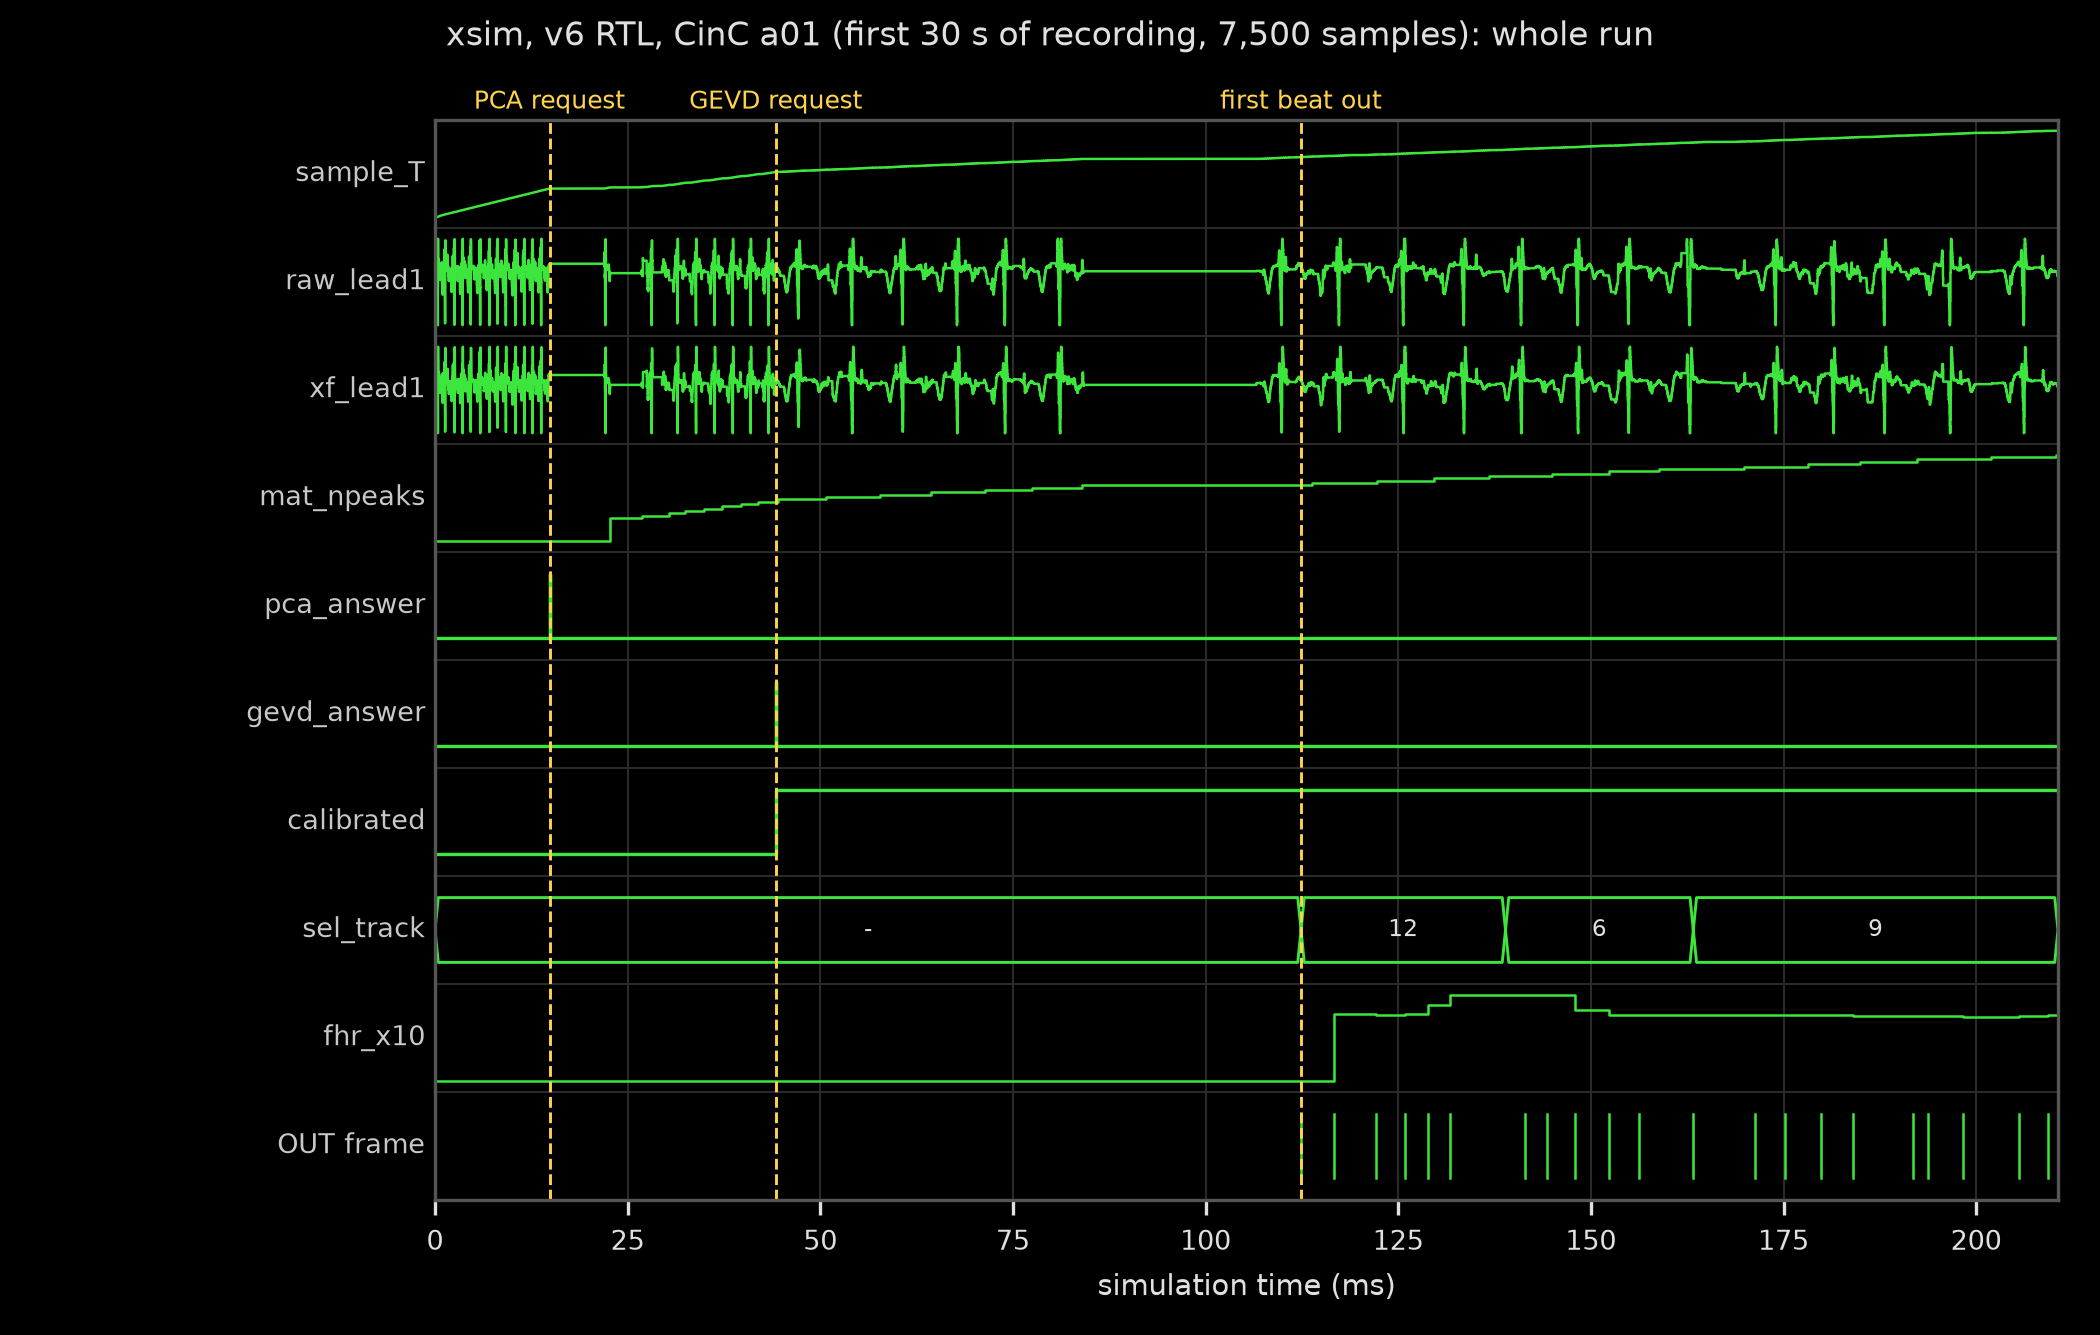
\includegraphics[width=0.92\textwidth]{figures/wave_overview.png}
\caption{\fb Whole simulation (210.6\,ms of simulated time for 30\,s of recording). The first 10\,s are processed quickly while the maternal-band samples are stored; then the PCA request goes to the PC, the stored 2,500 samples are replayed through the maternal detectors (flat \texttt{sample\_T}, rising \texttt{mat\_npeaks}), the GEVD request follows at 15\,s and sets \texttt{calibrated}. The long flat part of \texttt{sample\_T} at about 85--107\,ms is the one-time start of the beat trackers (an autocorrelation over 1,000 envelope samples per tracker). After that, the selected track (\texttt{sel\_track}), the FHR and the OUT frames appear. The analogue traces look uneven because the time axis is simulation time, not recording time.}
\label{fig:wave_overview}
\end{figure*}

\begin{figure*}[t]
\centering
\fb
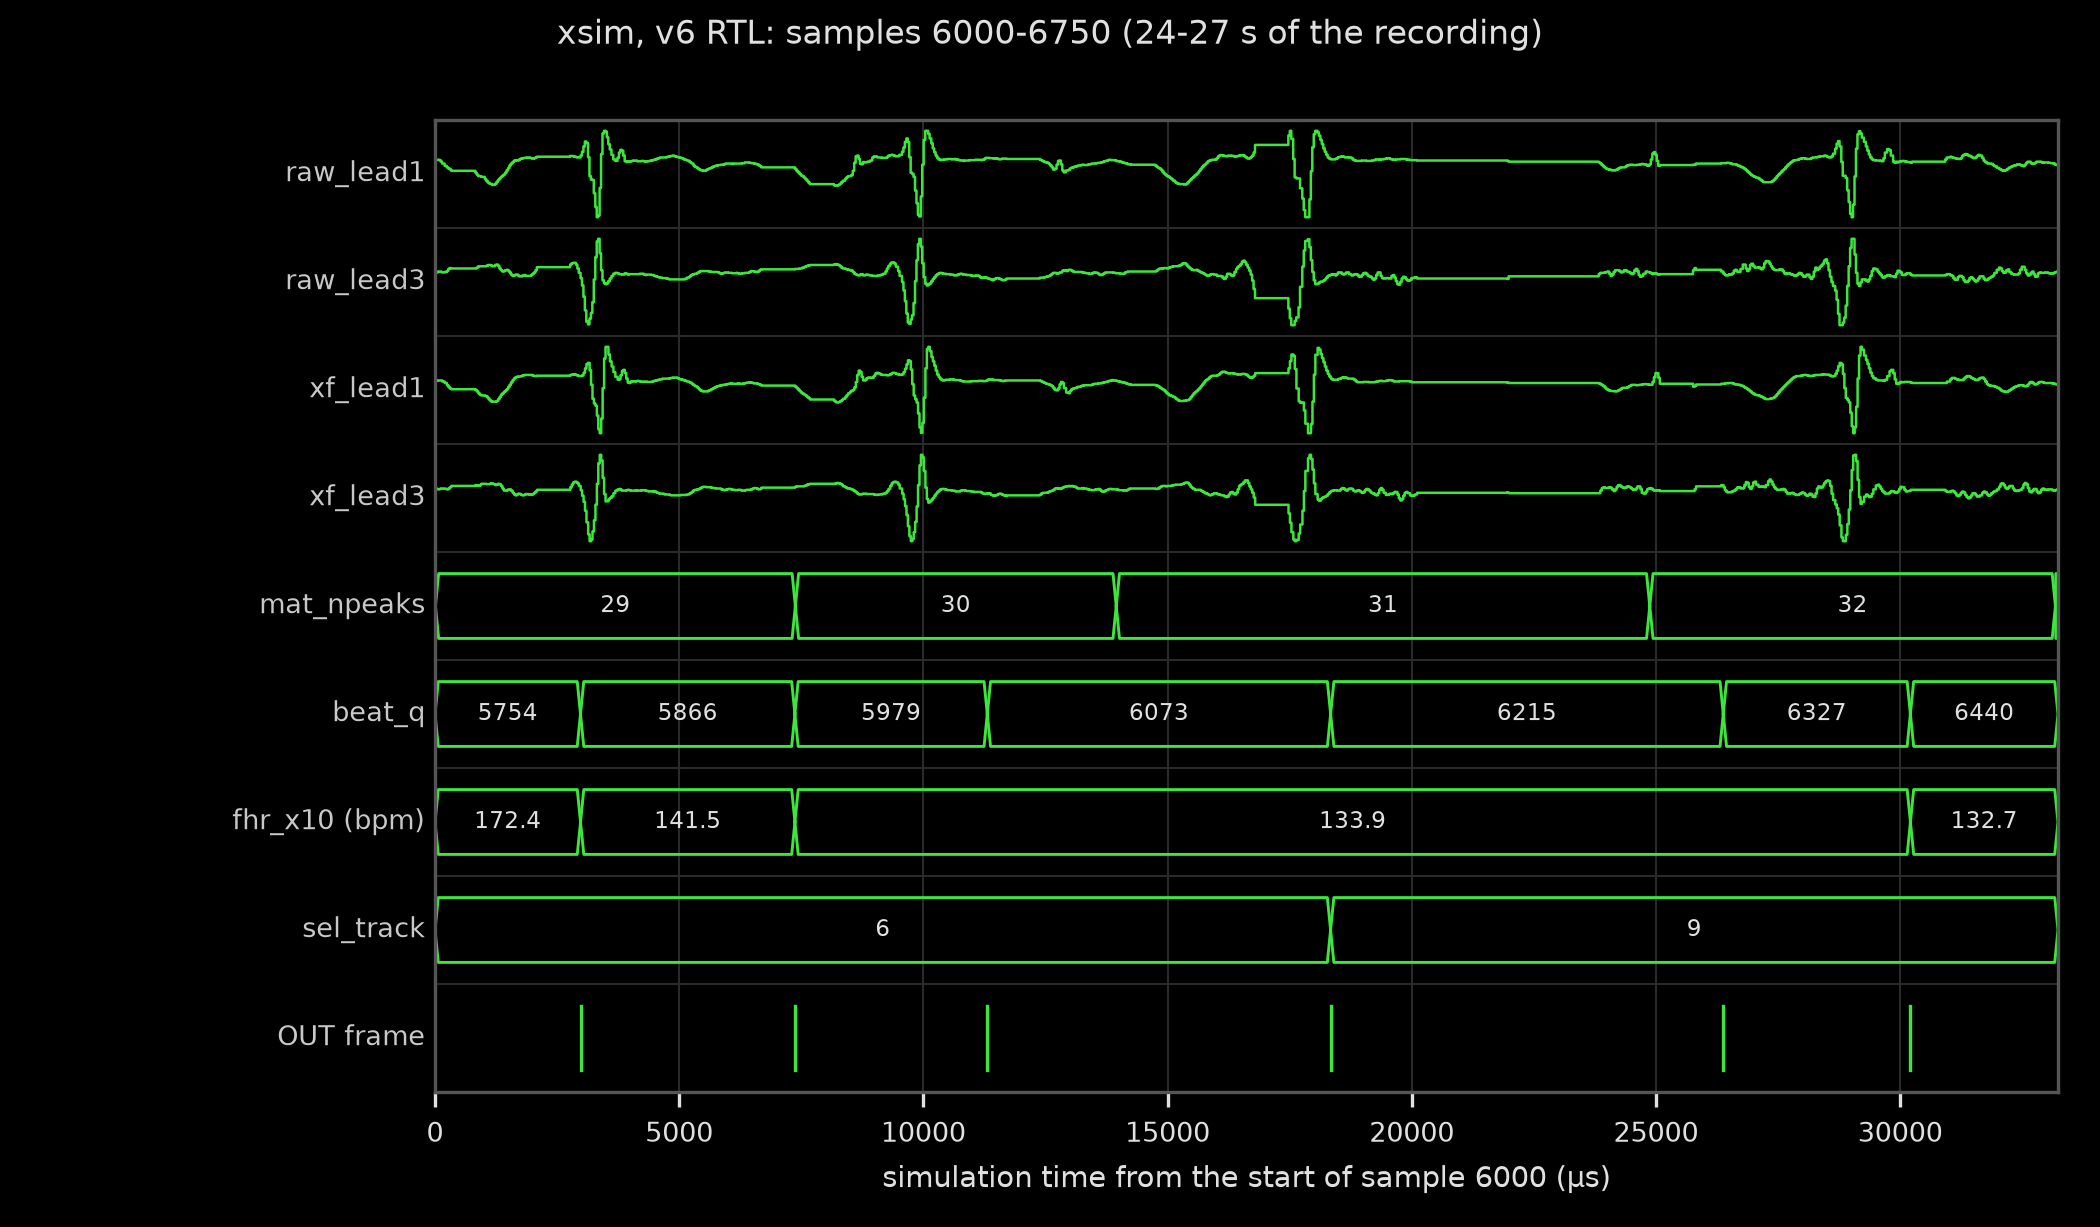
\includegraphics[width=0.92\textwidth]{figures/wave_signals.png}
\caption{\fb Three seconds of recording (samples 6,000--6,750) inside the RTL: raw input leads, front-end output $\mathbf{x}_f$, the maternal R-peak counter, the newest tracker beat (\texttt{beat\_q}, before the 13-sample latency compensation applied to the output), the FHR register in bpm, the selected track (which changes from 6 to 9 at a 2.5-s selection step) and the OUT frames sent to the PC.}
\label{fig:wave_signals}
\end{figure*}

\begin{figure*}[t]
\centering
\fb
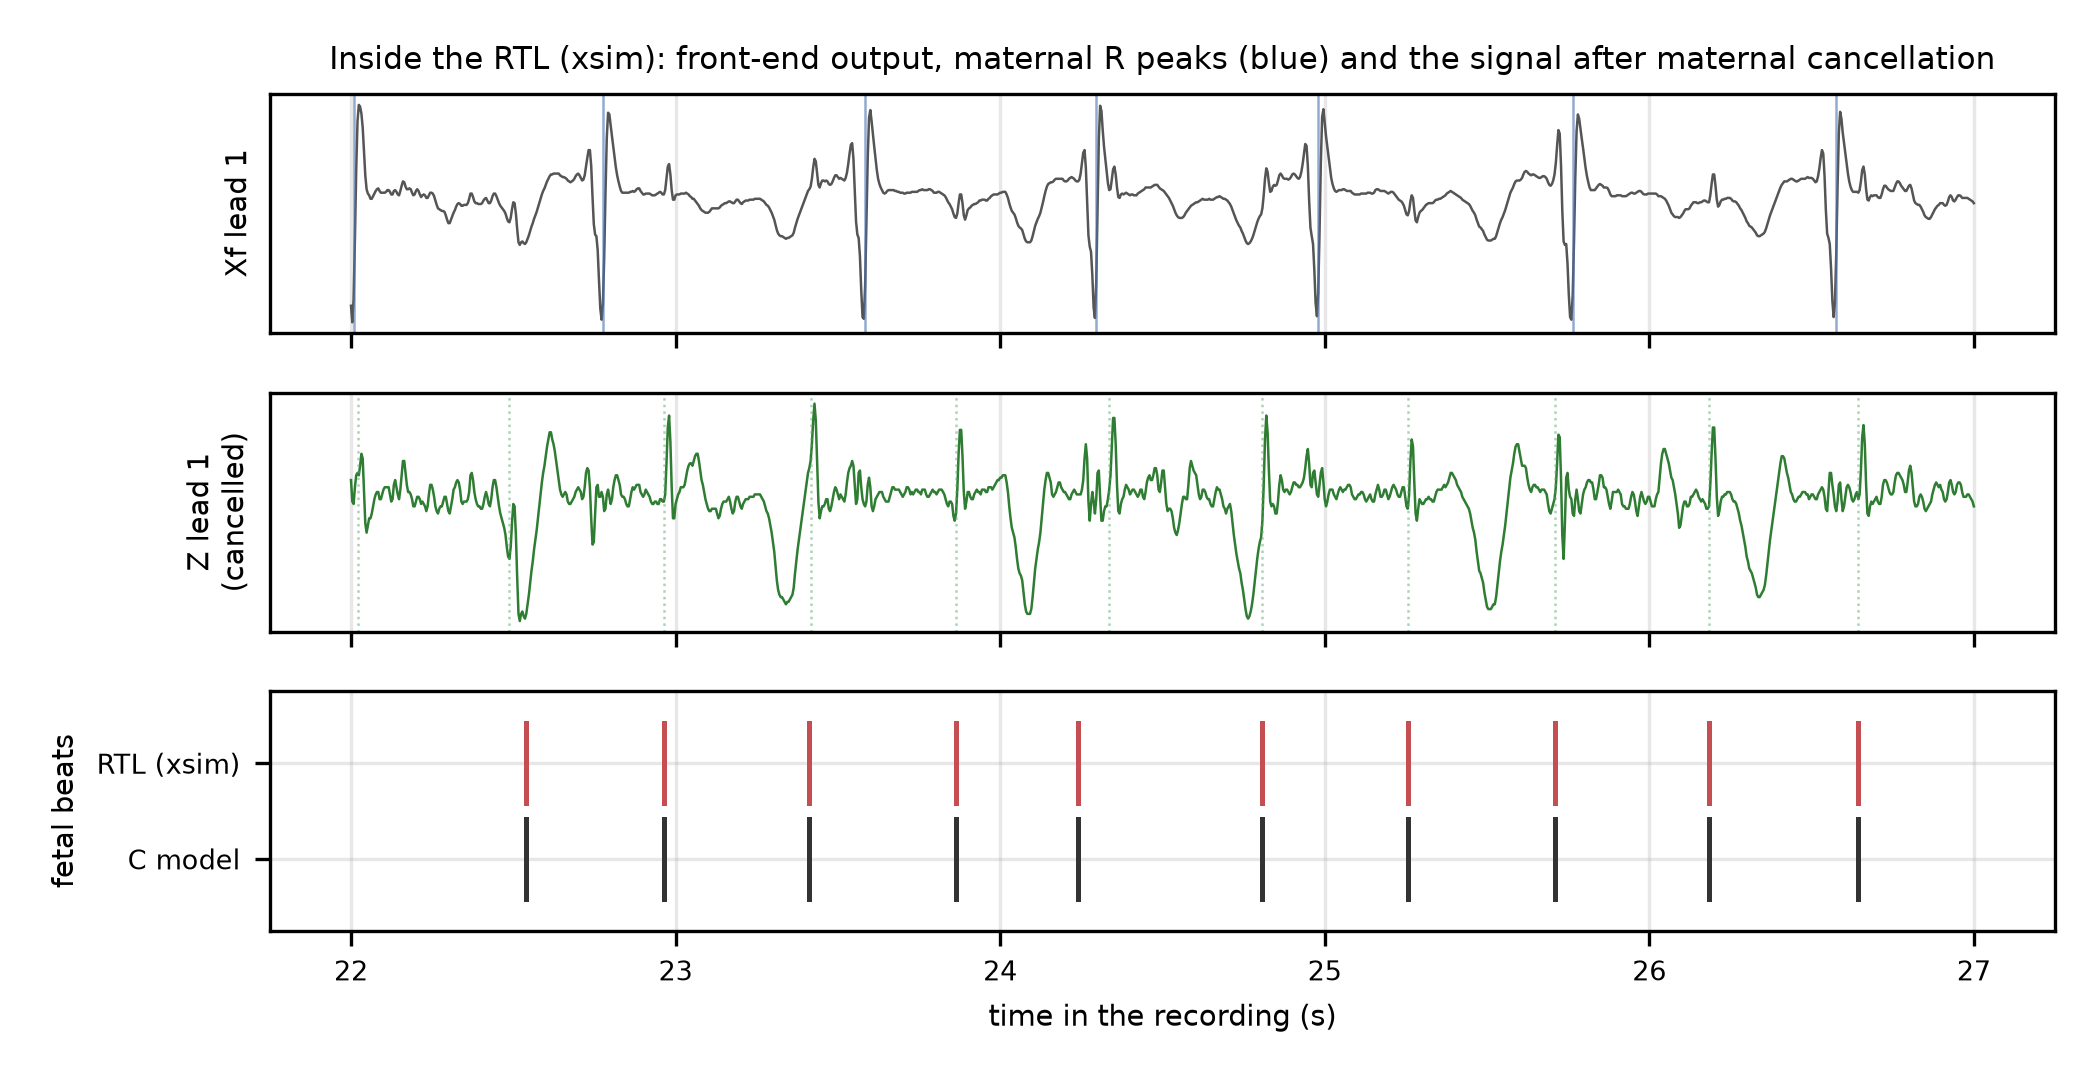
\includegraphics[width=0.92\textwidth]{figures/wave_cancellation.png}
\caption{\fb Maternal cancellation in the RTL, reconstructed from the simulated memory writes. Top: front-end output of lead 1 with the maternal R peaks found by the FPGA (blue). Middle: the same lead after per-beat maternal cancellation, as the tracks read it; the large maternal QRS complexes are gone and the small fetal complexes line up with the reference fetal annotations (dotted green). Bottom: fetal beats sent by the RTL and by the C model: identical.}
\label{fig:wave_canc}
\end{figure*}

\begin{figure*}[t]
\centering
\fb
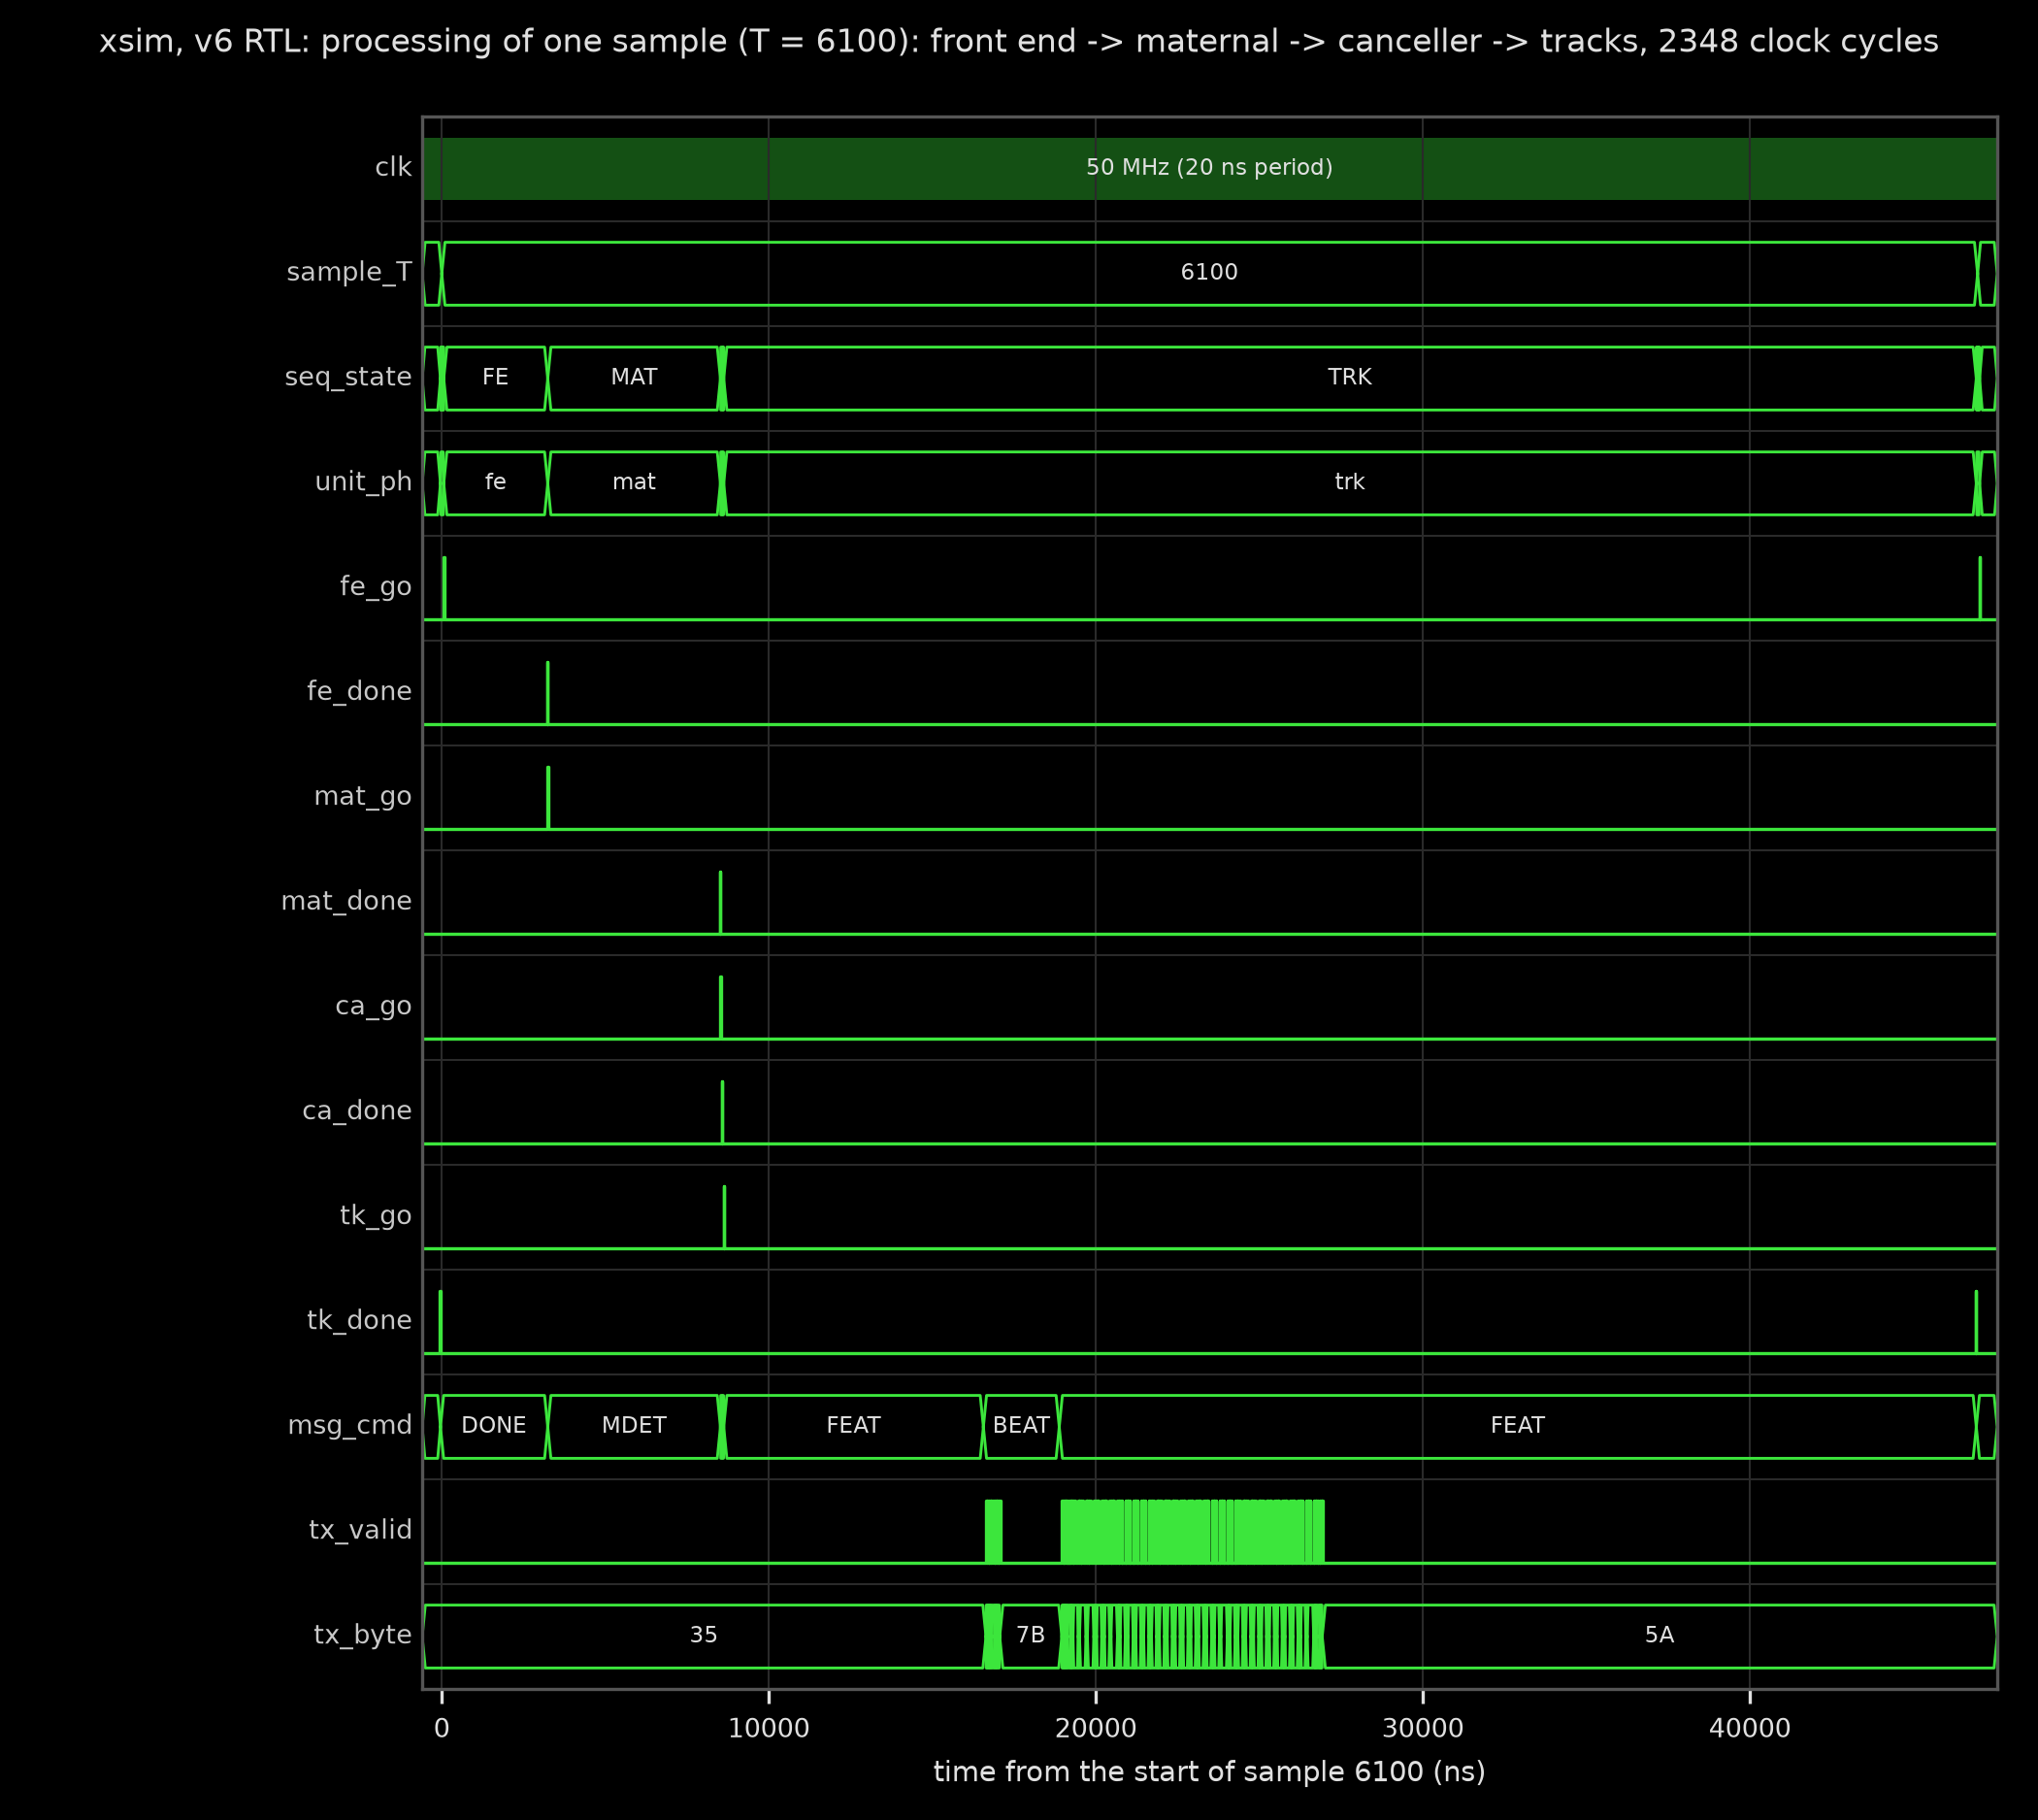
\includegraphics[width=0.92\textwidth]{figures/wave_one_sample.png}
\caption{\fb Clock-level view of one sample after calibration (T\,=\,6,100): the sequencer starts the front end, the maternal unit, the canceller (no maternal beat to process in this sample, so it finishes at once) and the 16-track unit, each with a go/done hand-shake; feature and beat frames are written to the UART buffer meanwhile. This sample takes 2,348 cycles ($47\,\mu$s at 50\,MHz).}
\label{fig:wave_sample}
\end{figure*}

\begin{figure}[t]
\centering
\fb
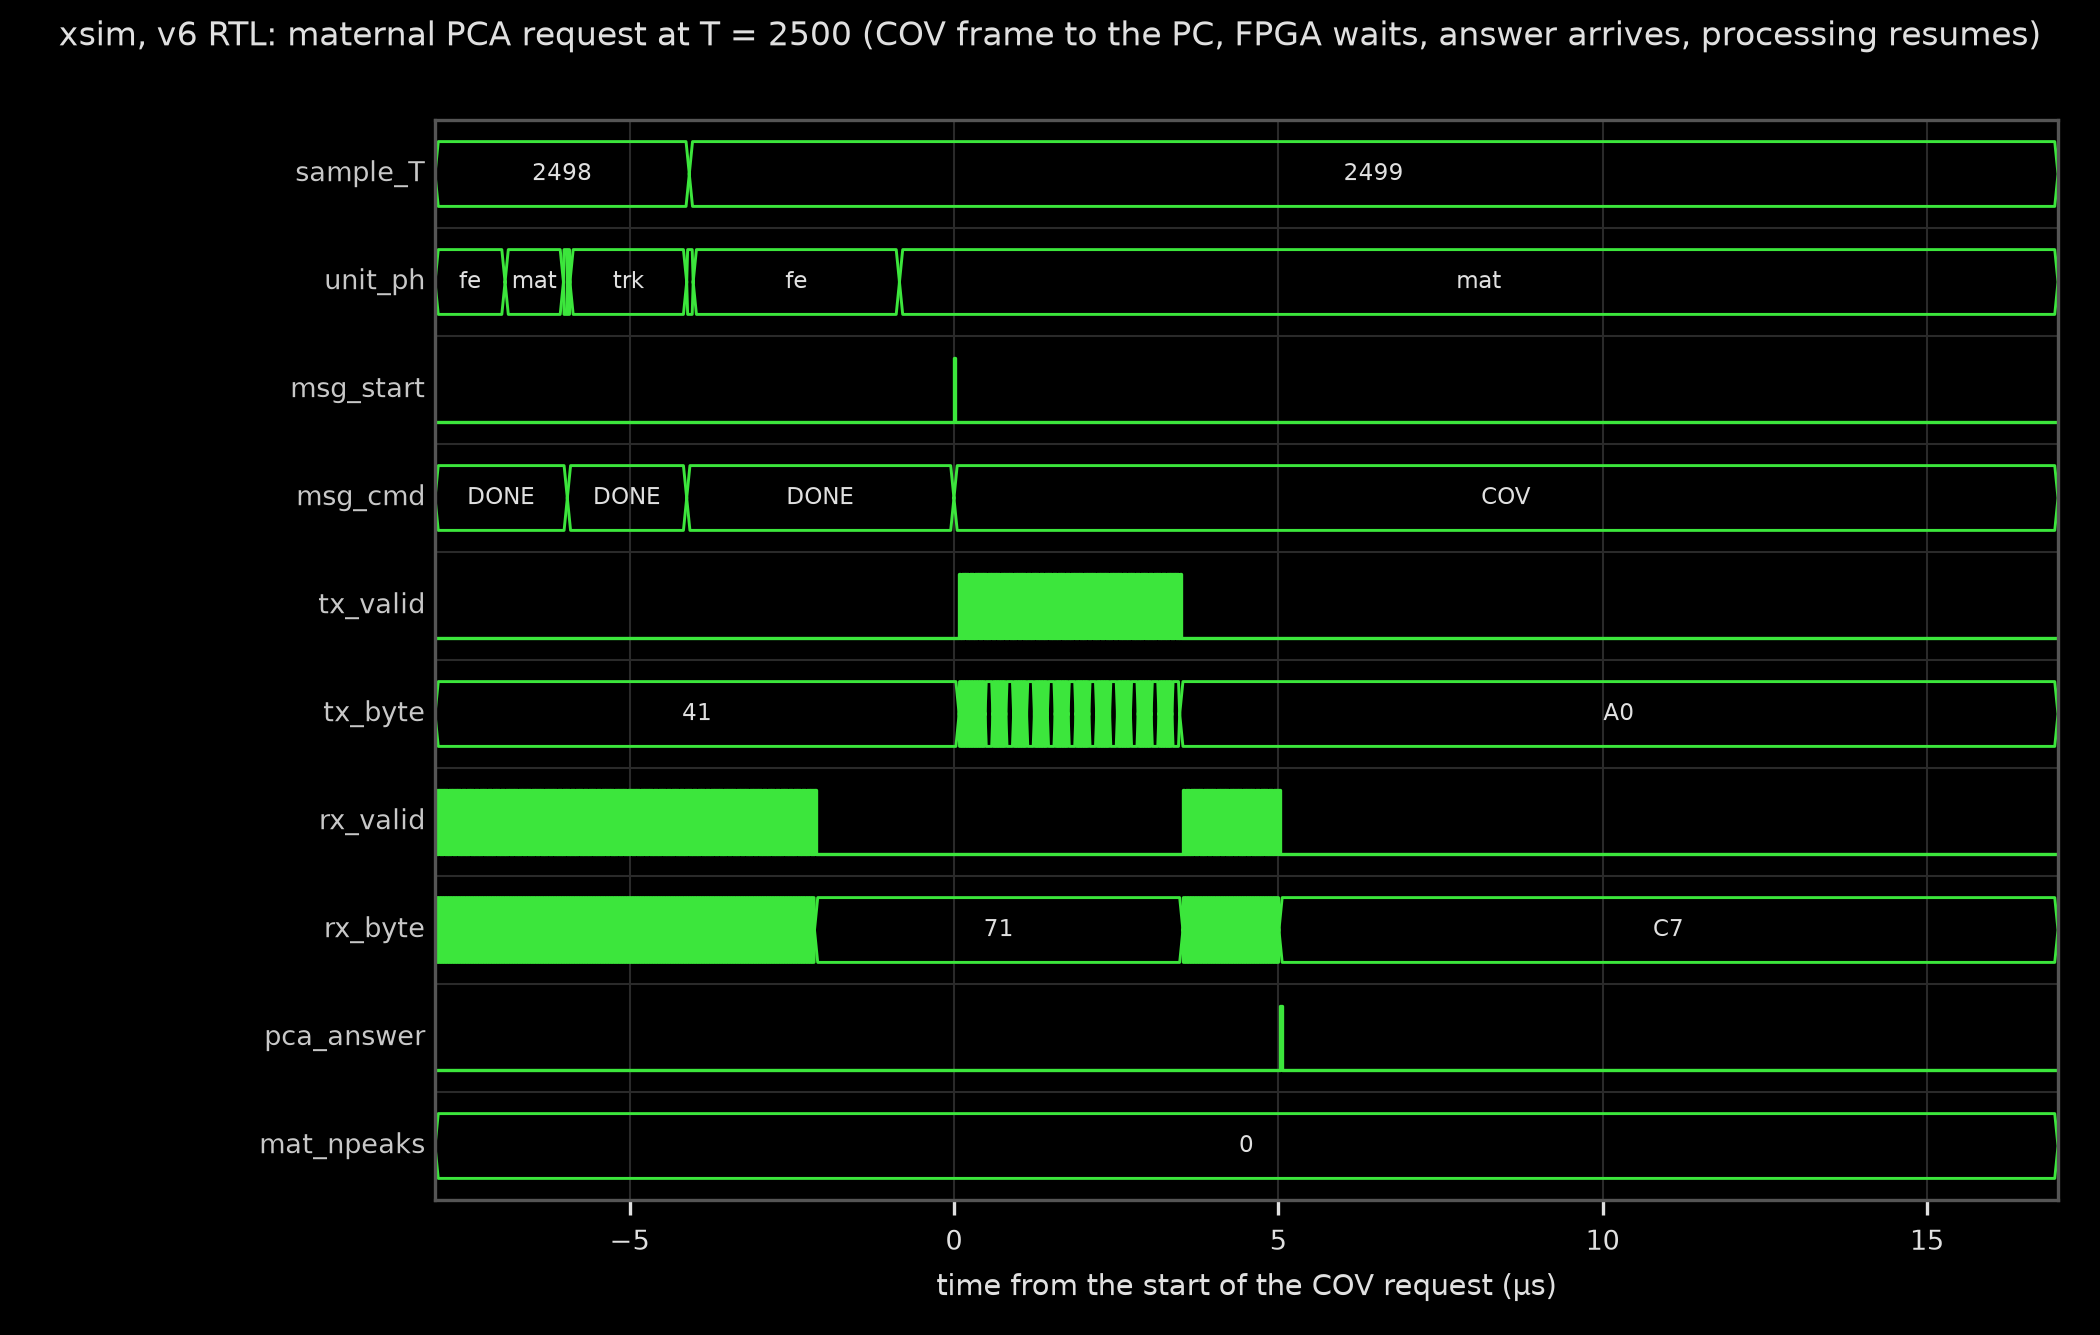
\includegraphics[width=\columnwidth]{figures/wave_pca_request.png}
\caption{\fb A request to the PC brain (maternal PCA at T\,=\,2,499): the maternal unit sends the COV frame (\texttt{tx\_valid}), the FPGA waits, the answer bytes arrive (\texttt{rx\_valid}), \texttt{pca\_answer} pulses and processing continues. Results therefore never depend on how fast the PC answers.}
\label{fig:wave_req}
\end{figure}

\begin{figure}[t]
\centering
\fb
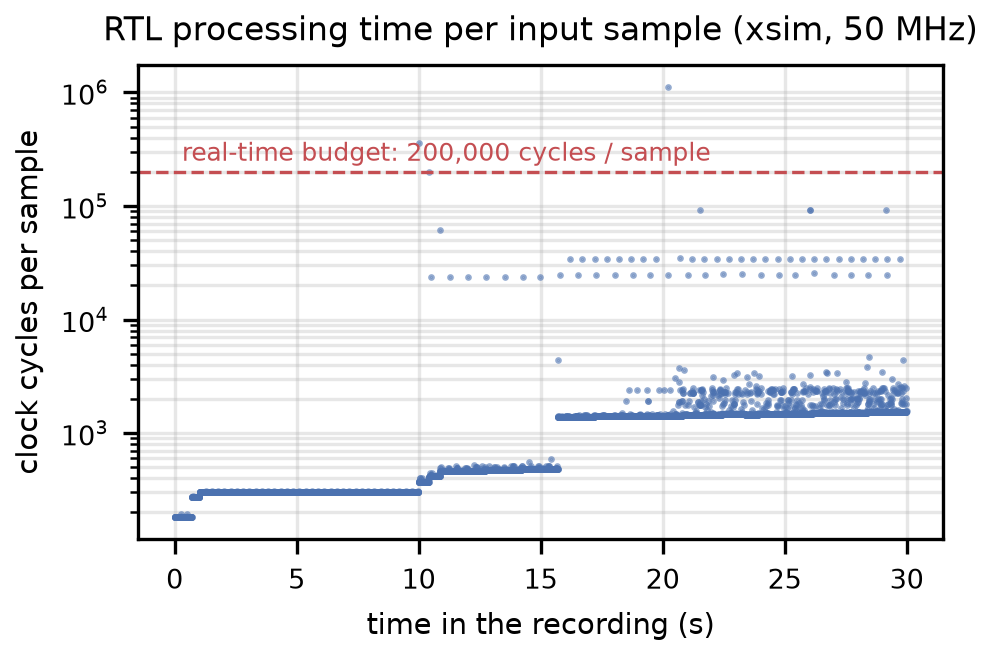
\includegraphics[width=\columnwidth]{figures/wave_cycles_per_sample.png}
\caption{\fb Clock cycles needed for each input sample in the simulation. Median 301 cycles before 10\,s, about 470 during calibration and 1,485 ($30\,\mu$s) once all 16 tracks run, far below the real-time budget of 200,000 cycles per sample. The single peak of 1.12 million cycles (22\,ms) is the tracker start; the 512-sample input FIFO absorbs it.}
\label{fig:wave_cycles}
\end{figure}

\noindent\textbf{Processing time per second of recording.} The 30\,s of recording took 210.6\,ms of simulated time, so the RTL alone runs about $140\times$ faster than real time (about 7\,ms of FPGA time per second of signal). On the board the system runs 4--5$\times$ real time (Sec.~\ref{sec:final_results}) because every sample and every PC request also has to cross the 921,600-baud UART and wait for the PC; the FPGA logic is not the bottleneck.

\begin{figure*}[t]
\centering
\fb
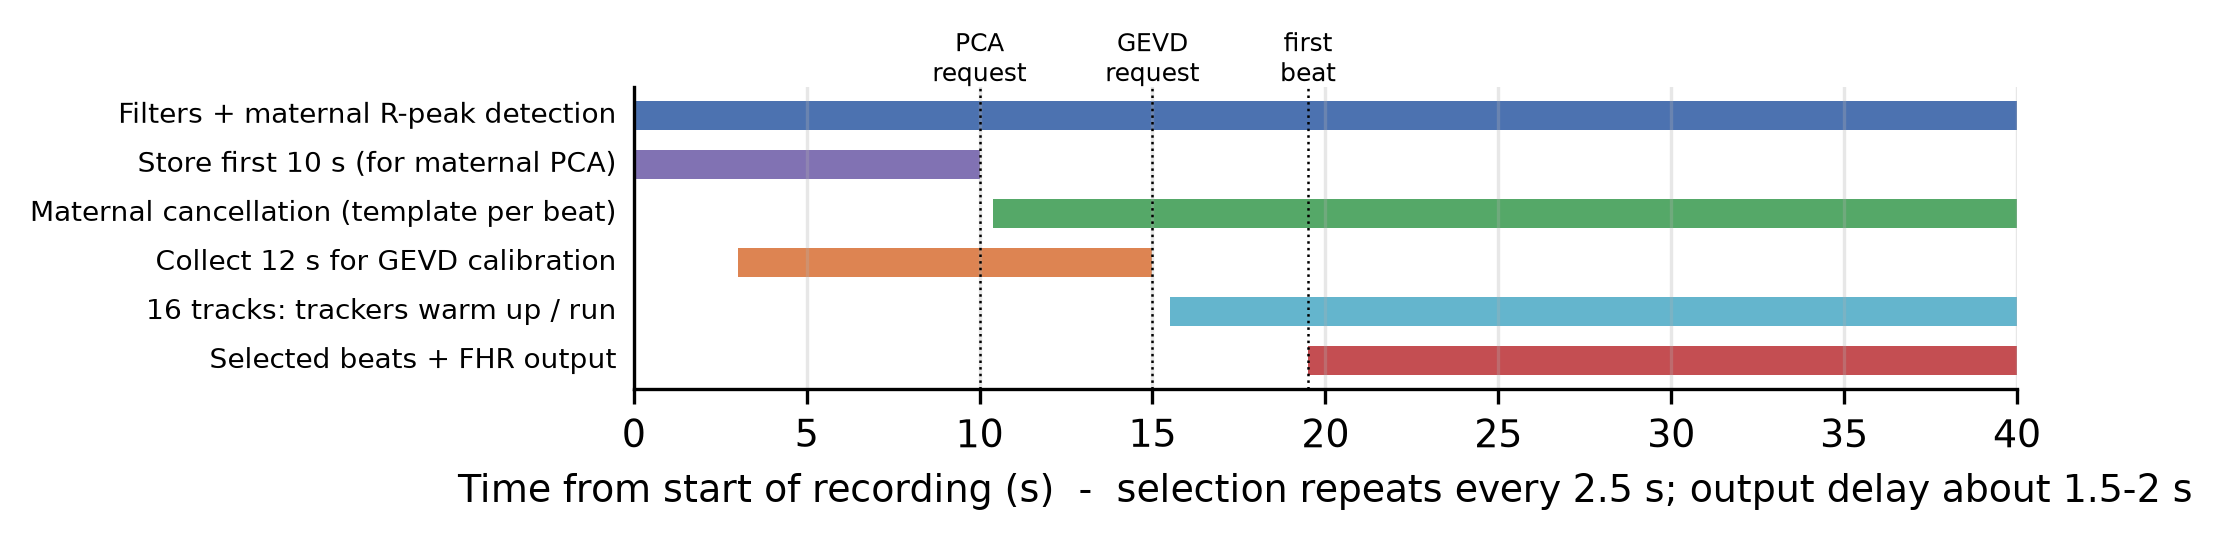
\includegraphics[width=0.92\textwidth]{figures/fin_startup_timeline.png}
\caption{\fb Start-up timeline of v6 on a recording. The first $10\,$s are stored for the maternal PCA, the GEVD calibration uses $[3, 15)\,$s, and the first selected beat comes out at about $19.5\,$s. After that a new track decision is made every $2.5\,$s. Each beat is reported about $1.5$--$2\,$s after it happens (tracker confirmation plus the selection delay); this is why scoring starts at $20\,$s.}
\label{fig:fin_timeline}
\end{figure*}

\noindent\textbf{Implementation.} Vivado builds the design for the XC7S50 with a PLL from the 100\,MHz board clock to 50\,MHz. Two changes were needed for implementation: the $\mathbf{z}$ ring was merged to a single write port so that it maps to block RAM, and a sorting-network loop was rewritten to pass synthesis.

\noindent\textbf{Block RAM reduction.} The first v6 build used 74.5 of 75 BRAM tiles ($99\%$). The two largest memories were the 10-s maternal-band store for the PCA (14.5 tiles, used only before $10\,$s) and the 16 envelope rings of the trackers (16 tiles, written only after calibration). Their lifetimes never overlap, and the largest envelope code is 7,423 ($< 2^{13}$), so both now share one $32\text{K} \times 13$ memory. We proved that stale data is never read in two ways: the C model with the envelope rings filled with garbage at calibration gives identical outputs on 80 records, and the RTL regression and all 140 board records give byte-identical output streams (same MD5) before and after the change. Two other ideas were checked and rejected: the 4096-deep sample rings are needed for the start-up burst of cancellations at $\approx 10.4\,$s, and the envelope rings cannot be halved because a tracker restart looks back up to about 1,057 samples.

\begin{table}[t]
\fb
\caption{\fb FPGA utilisation of the v6 design on the XC7S50 (Vivado post-implementation), before and after sharing the block RAM. v6.1 and v7-DL: Tab.~\ref{tab:v7_hw}.}
\label{tab:final_resources}
\centering
\resizebox{\columnwidth}{!}{%
\begin{tabular}{@{}lccc@{}}
\toprule
\textbf{Resource} & \textbf{Available} & \textbf{v6 first build} & \textbf{v6, shared BRAM} \\
\midrule
LUTs & 32,600 & 19.0k (58\%) & \textbf{18,127 (55.6\%)} \\
Flip-flops & 65,200 & 10.1k (16\%) & \textbf{10,015 (15.4\%)} \\
DSP48E1 & 120 & 33 (27.5\%) & \textbf{33 (27.5\%)} \\
Block RAM tiles & 75 & 74.5 (99\%) & \textbf{60 (80\%)} \\
Clock / worst slack & -- & 50\,MHz / +0.49\,ns & \textbf{50\,MHz / +0.26\,ns} \\
On-chip power (estimate) & -- & -- & \textbf{0.374\,W} \\
\bottomrule
\end{tabular}%
}
\end{table}

\noindent\textbf{Where the resources go.} \Cref{tab:module_resources} splits v6 by Verilog module (Vivado hierarchical utilisation). The 16-track block is more than half of the logic: it holds the projections, the 12 trackers with their autocorrelation and sorting networks, the threshold detectors and the selection features. The core's 28 BRAM tiles are the two 4096-sample rings for $\mathbf{x}_f$ and $\mathbf{z}$ and the shared $32\text{K}\times 13$ memory. Many small per-track and per-detector state variables are stored in LUT RAM (2,142 LUTs).

\begin{table}[t]
\fb
\caption{\fb Resources per module of v6 (post-implementation). BRAM in 36-kb tiles (one RAMB18 counts as half a tile).}
\label{tab:module_resources}
\centering
\resizebox{\columnwidth}{!}{%
\begin{tabular}{@{}llrrrrr@{}}
\toprule
\textbf{Module} & \textbf{Function} & \textbf{LUTs} & \textbf{of which RAM} & \textbf{FFs} & \textbf{BRAM} & \textbf{DSP} \\
\midrule
\texttt{v6\_trk} & 16 tracks, trackers, selection, output & 10,046 & 1,230 & 3,400 & 14 & 10 \\
\texttt{v6\_mat} & maternal PCA hand-shake, detectors & 4,921 & 862 & 2,582 & 3 & 4 \\
\texttt{v6\_canc} & maternal cancellation & 1,144 & 50 & 948 & 10.5 & 15 \\
\texttt{v6\_link} & frames, FIFOs, PC answer buffers & 883 & 0 & 1,825 & 3.5 & 0 \\
\texttt{v6\_fe} & front-end filters & 799 & 0 & 959 & 1 & 4 \\
\texttt{v6\_core} (own) & sequencer, rings, shared memory & 291 & 0 & 231 & 28 & 0 \\
\midrule
\textbf{Total} (incl.\ top) & & \textbf{18,127} & \textbf{2,142} & \textbf{10,015} & \textbf{60} & \textbf{33} \\
\bottomrule
\end{tabular}%
}
\end{table}

\noindent\textbf{Power.} The mid-term report could only give an analytical power estimate. Vivado's power analysis of the routed v6 design (default switching activity, no measured activity file, confidence ``medium'') gives $0.374\,$W total on-chip power: $0.299\,$W dynamic (of which the PLL $0.097\,$W, signals $0.065\,$W, logic $0.058\,$W, block RAM $0.050\,$W, DSP $0.015\,$W) and $0.075\,$W static, at a junction temperature of $26.8\,^\circ$C. This is well inside the $1.5\,$W wearable budget of \cref{tab:clinical_specs} (v7-DL: $0.445\,$W); it does not include the rest of the board, which we did not measure.

\begin{figure}[t]
\centering
\fb
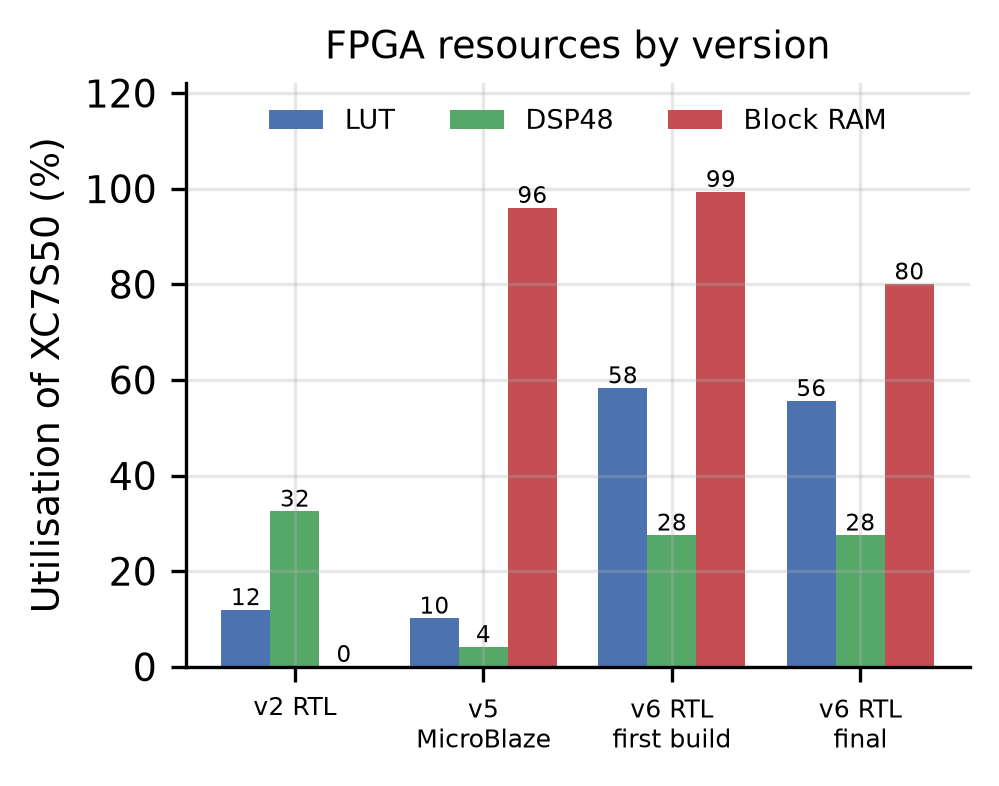
\includegraphics[width=\columnwidth]{figures/fin_fpga_resources.png}
\caption{\fb FPGA utilisation of each hardware version. v2 needed little logic because the PC computed the weights; v5 filled the block RAM with processor memory; v6 does all the work in logic and, after sharing one memory, leaves 15 BRAM tiles free.}
\label{fig:fin_resources}
\end{figure}

% =====================================================================
\section{Board Results of v6}
\label{sec:final_results}

The PC streams each recording (int16, 4 leads, 250\,Hz) to the board in 64-sample frames and runs the brain; the RTL does everything else. For every record the board's complete output byte stream is also compared with the C model.

\begin{table*}[t]
\fb
\caption{\fb Results of v6 measured on the Spartan-7 board (140 records). Every record was bit-exact with the C model. ``$\ge 90\%$'' counts records with F1 of at least $90\%$. Speed is total record length divided by total streaming time, including UART transfer and the PC brain. The last row is the C model on all FECGSYNDB records (identical to the board wherever both were run).}
\label{tab:final_results}
\centering
\resizebox{\textwidth}{!}{%
\begin{tabular}{@{}lcccccccc@{}}
\toprule
\textbf{Data set} & \textbf{Records} & \textbf{F1 (\%)} & \textbf{Se (\%)} & \textbf{PPV (\%)} & \textbf{FHR MAE (bpm)} & \textbf{Records $\ge 90\%$} & \textbf{Bit-exact} & \textbf{Speed} \\
\midrule
FECGSYNDB subset (synthetic) & 60 & 91.83 & 90.67 & 93.65 & 5.24 & 42 & 60/60 & 4.3$\times$ \\
ADFECGDB (real, scalp reference) & 5 & 92.73 & 91.16 & 94.37 & 2.03 & 4 & 5/5 & 4.6$\times$ \\
CinC 2013 dev (real, odd records) & 38 & 76.04 & 74.45 & 77.98 & 12.52 & 13 & 38/38 & 4.8$\times$ \\
\textbf{CinC 2013 test (real, held out)} & \textbf{37} & \textbf{65.48} & \textbf{64.39} & \textbf{67.00} & \textbf{18.37} & \textbf{13} & \textbf{37/37} & \textbf{5.1$\times$} \\
\midrule
FECGSYNDB all (C model) & 1,248 & 91.44 & -- & -- & -- & -- & -- & -- \\
\quad by condition & \multicolumn{8}{l}{$c0$ 96.8, $c1$ 96.9, $c2$ 91.7, $c3$ 93.3, $c4$ 78.5} \\
\bottomrule
\end{tabular}%
}
\end{table*}

\begin{figure}[t]
\centering
\fb
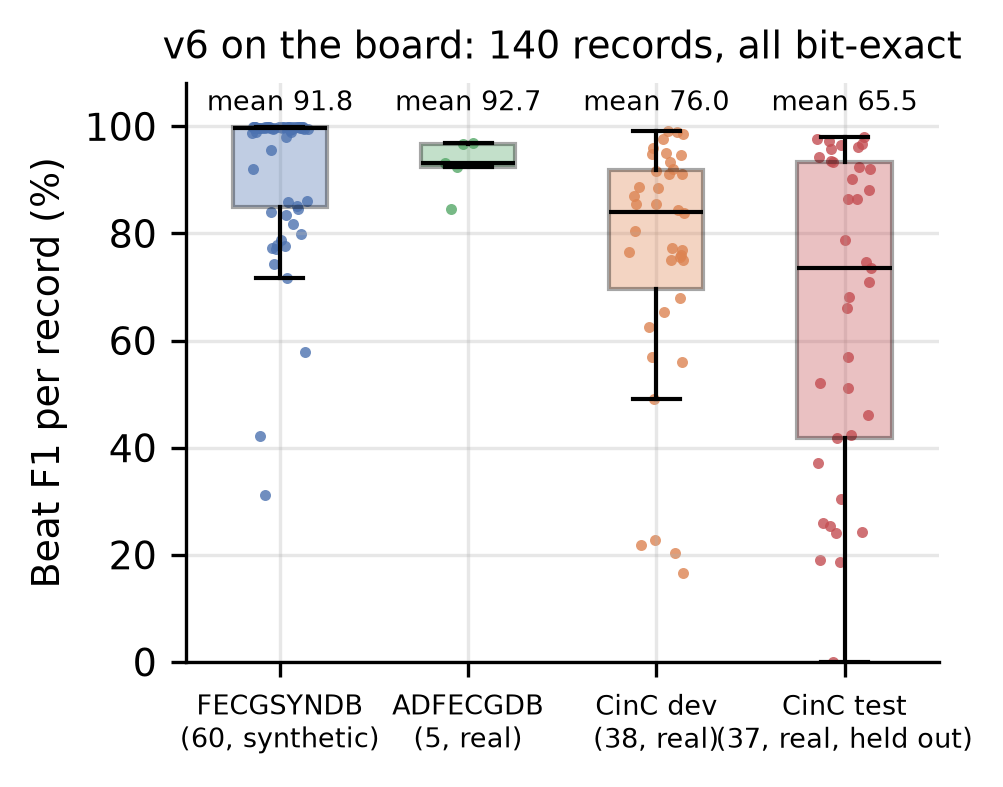
\includegraphics[width=\columnwidth]{figures/fin_board_f1_distribution.png}
\caption{\fb Per-record F1 of v6 on the board. Most synthetic and ADFECGDB records are above $90\%$; real CinC recordings spread from $0$ to $99\%$, so the mean hides a large difference between easy and hard recordings (CinC test median $73.6\%$, dev median $84.1\%$).}
\label{fig:fin_dist}
\end{figure}

\begin{figure}[t]
\centering
\fb
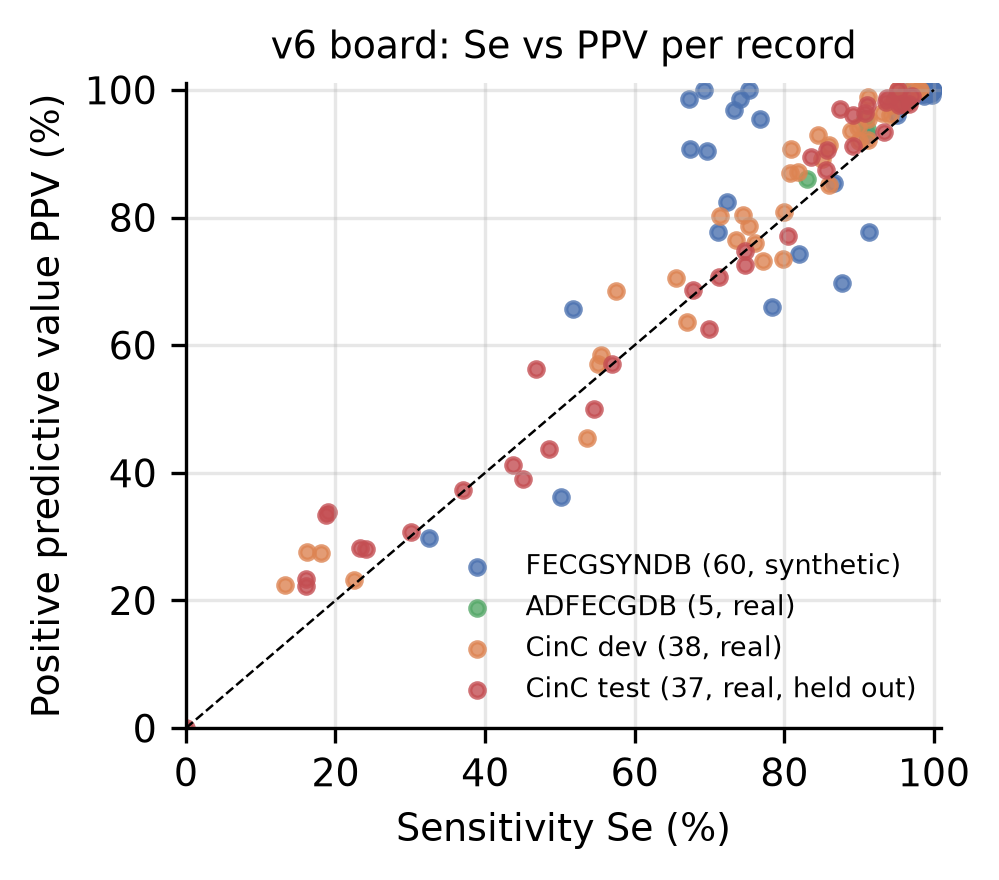
\includegraphics[width=\columnwidth]{figures/fin_board_se_ppv.png}
\caption{\fb Sensitivity against positive predictive value per record on the board. Failed real recordings lie close to the diagonal (Se and PPV both low): the design followed a wrong train, often the mother or noise. Weaker synthetic records have high PPV but lower Se: the reported beats are right, but some are missed (e.g.\ ectopic beats).}
\label{fig:fin_seppv}
\end{figure}

\begin{figure*}[t]
\centering
\fb
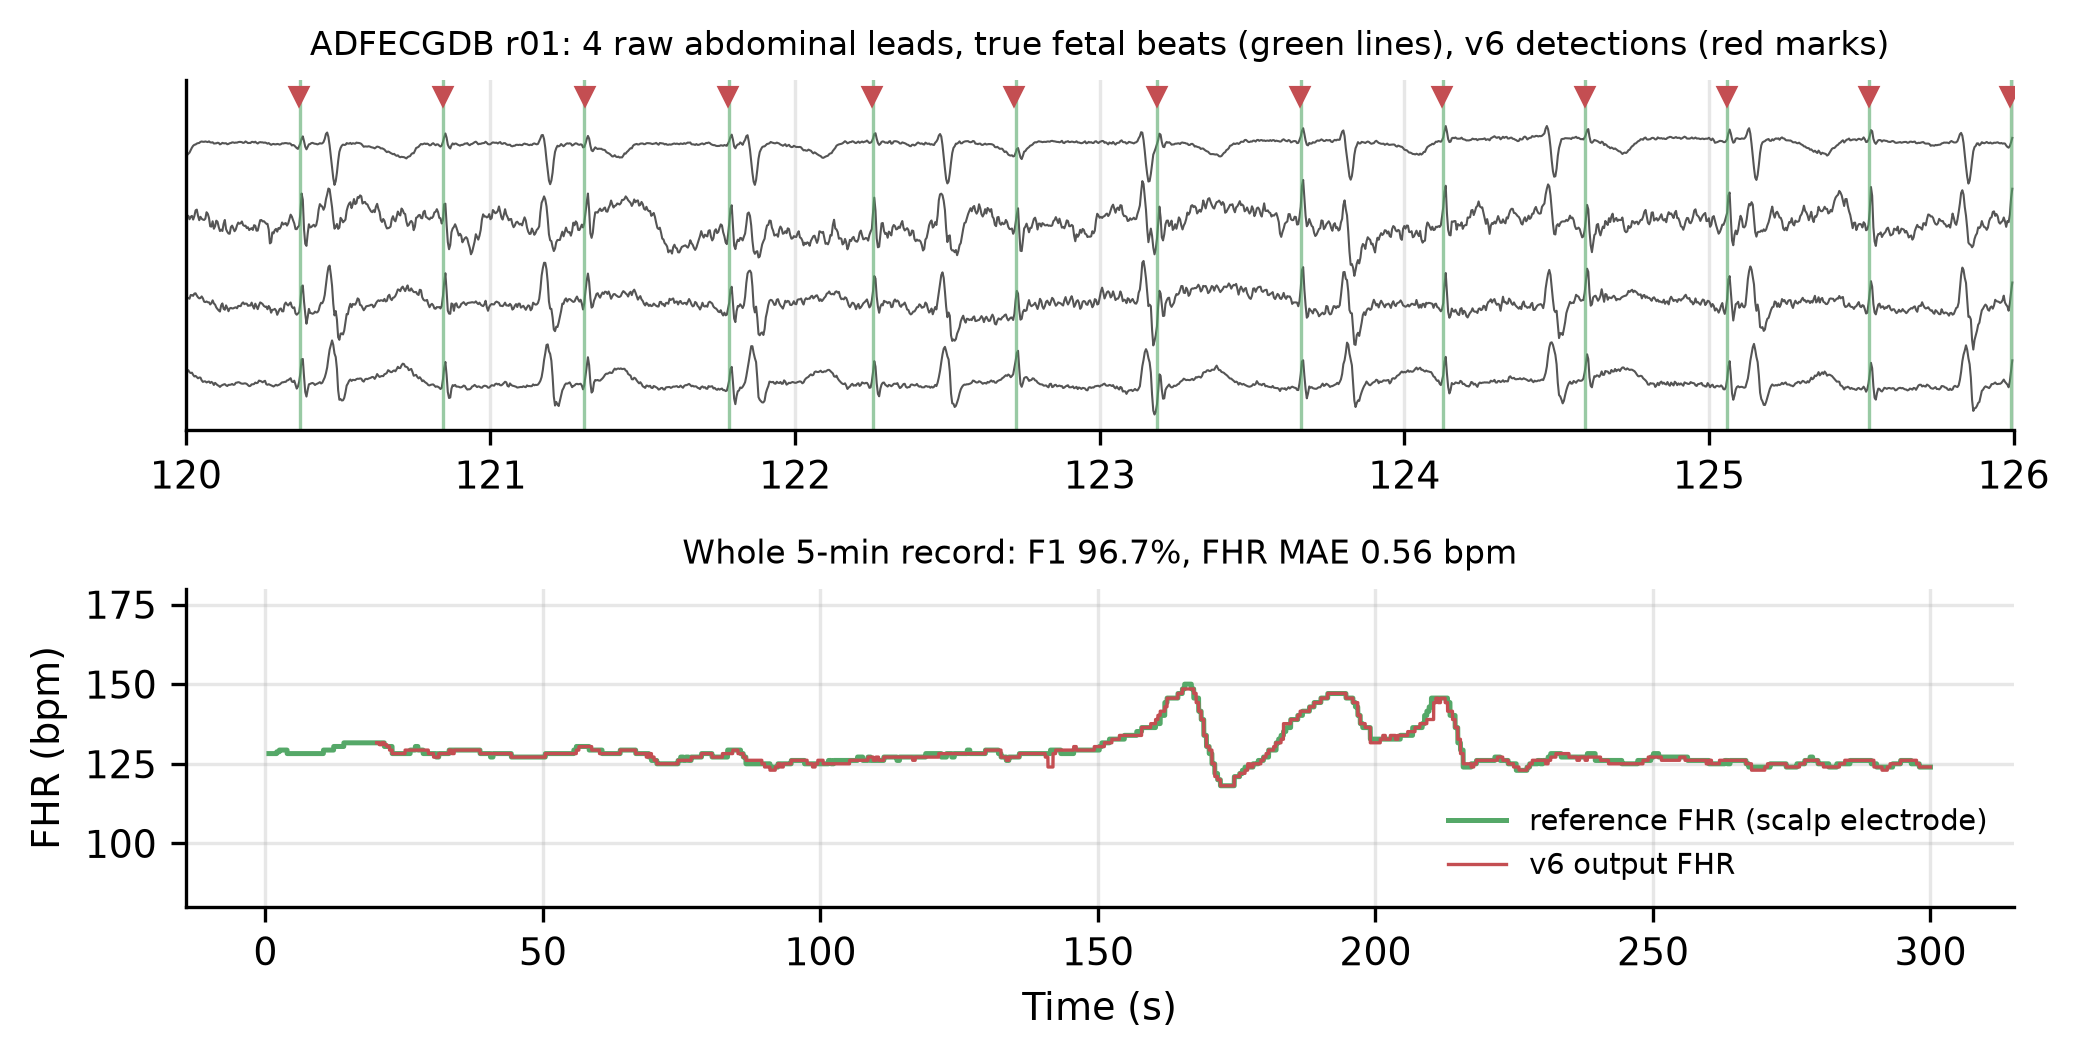
\includegraphics[width=0.92\textwidth]{figures/fin_fhr_trace_r01.png}
\caption{\fb Example output on a real recording (ADFECGDB r01, 5\,min), from the C model, which is bit-exact with the board. Top: 6\,s of the four raw abdominal leads, where the large complexes are maternal; green lines are the true fetal beats from the scalp electrode and red marks are v6 detections. Bottom: v6 FHR against the reference over the whole record (F1 $96.7\%$, FHR MAE $0.56\,$bpm), including the accelerations at 160--215\,s.}
\label{fig:fin_trace}
\end{figure*}

\begin{figure}[t]
\centering
\fb
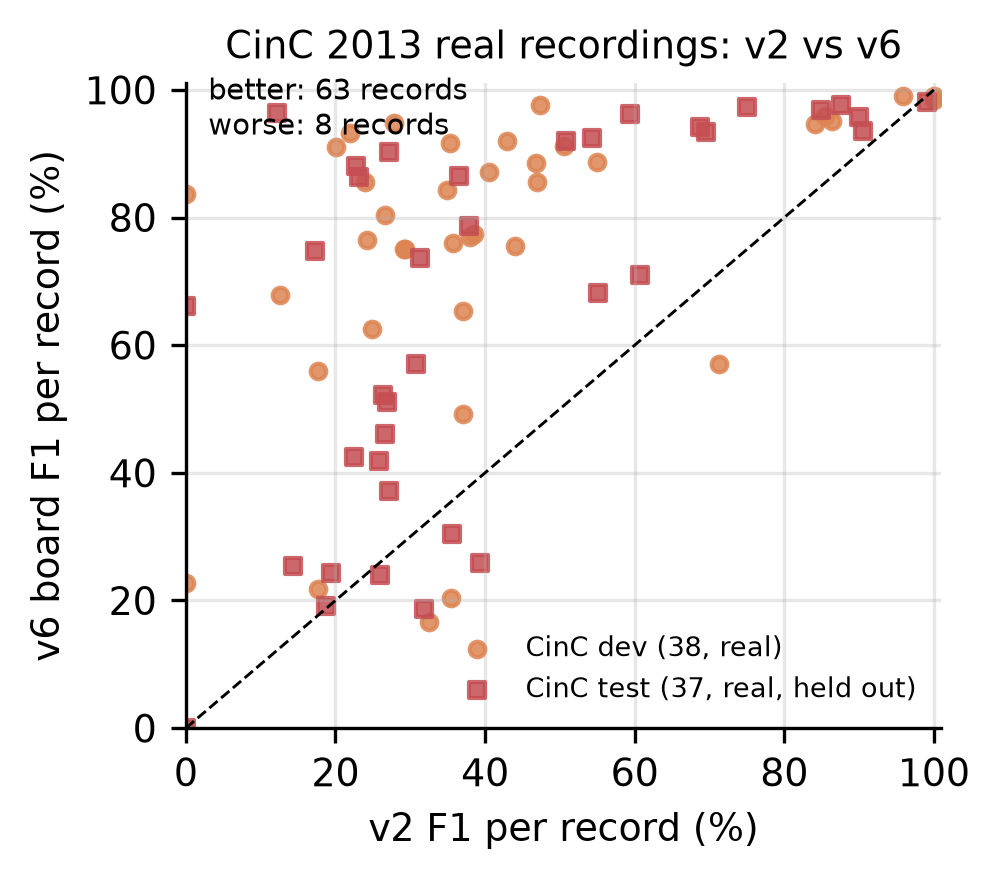
\includegraphics[width=\columnwidth]{figures/fin_cinc_v2_vs_v6.png}
\caption{\fb The same 75 real CinC recordings with v2 and with v6 (board). 63 records improve by more than one point and 8 get worse; the gain is not limited to a few records.}
\label{fig:fin_cinc}
\end{figure}

\begin{figure*}[t]
\centering
\fb
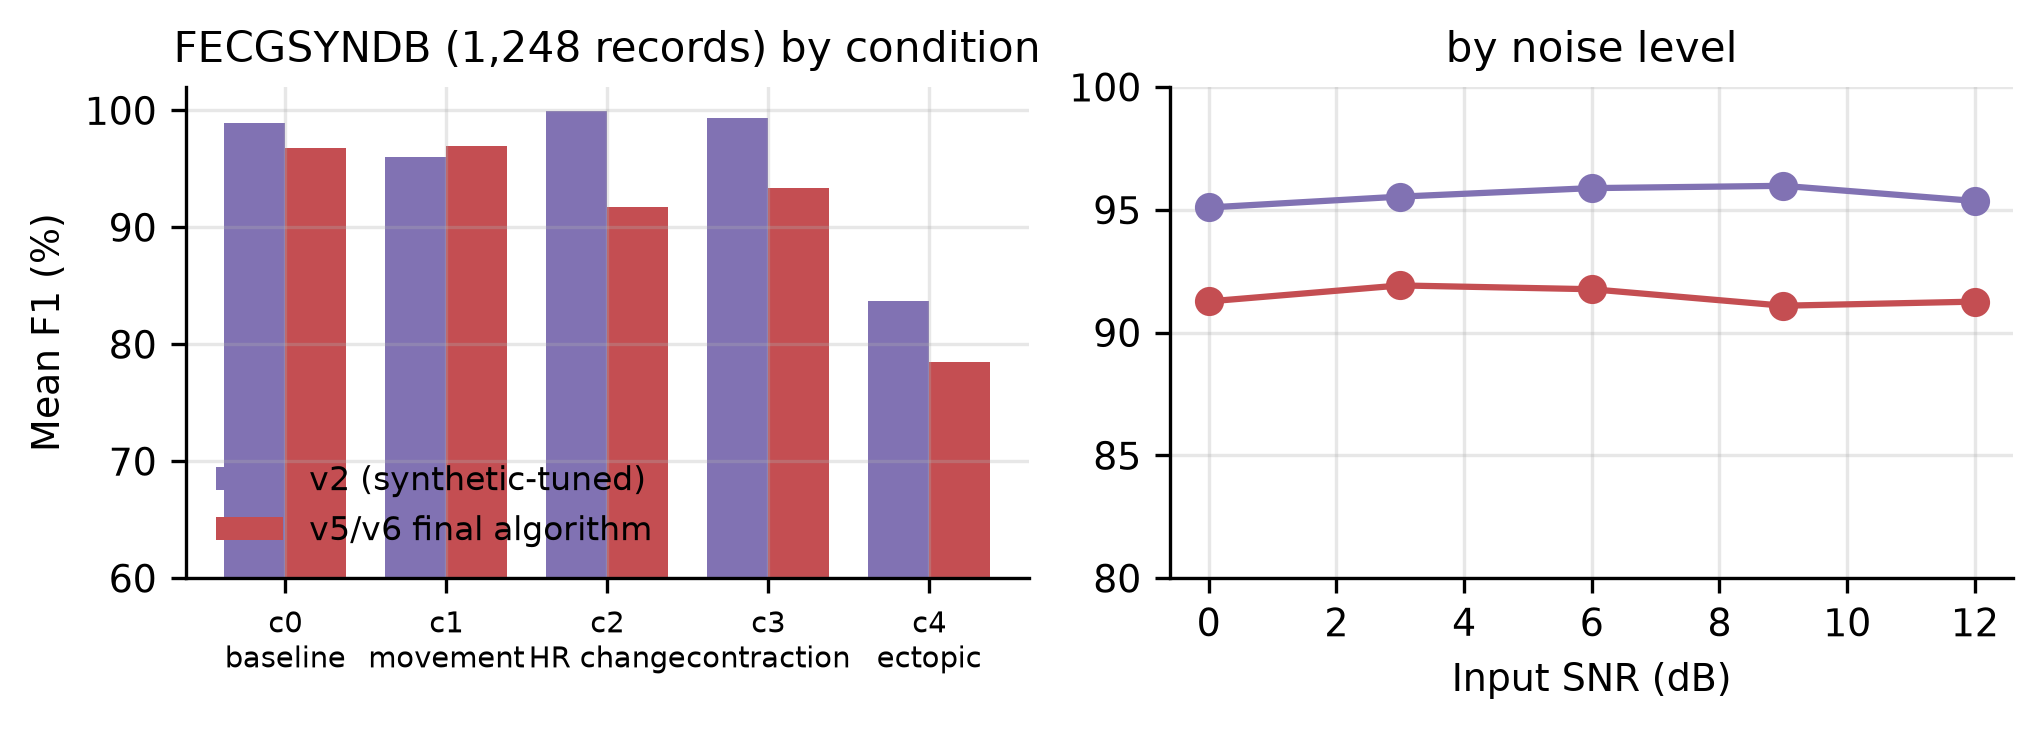
\includegraphics[width=0.92\textwidth]{figures/fin_syn_condition_snr.png}
\caption{\fb FECGSYNDB (1,248 records) by clinical condition and by input SNR for v2 and for the final algorithm (C model of v5; v6 differs by at most $0.1$ point on every condition). The final algorithm loses on heart-rate changes ($c2$), contractions ($c3$) and ectopic beats ($c4$), where the RR-regularity term and the FHR prior can penalise the true fetal track, and is almost flat across SNR ($91.1$--$91.9\%$).}
\label{fig:fin_syn}
\end{figure*}

\begin{figure*}[t]
\centering
\fb
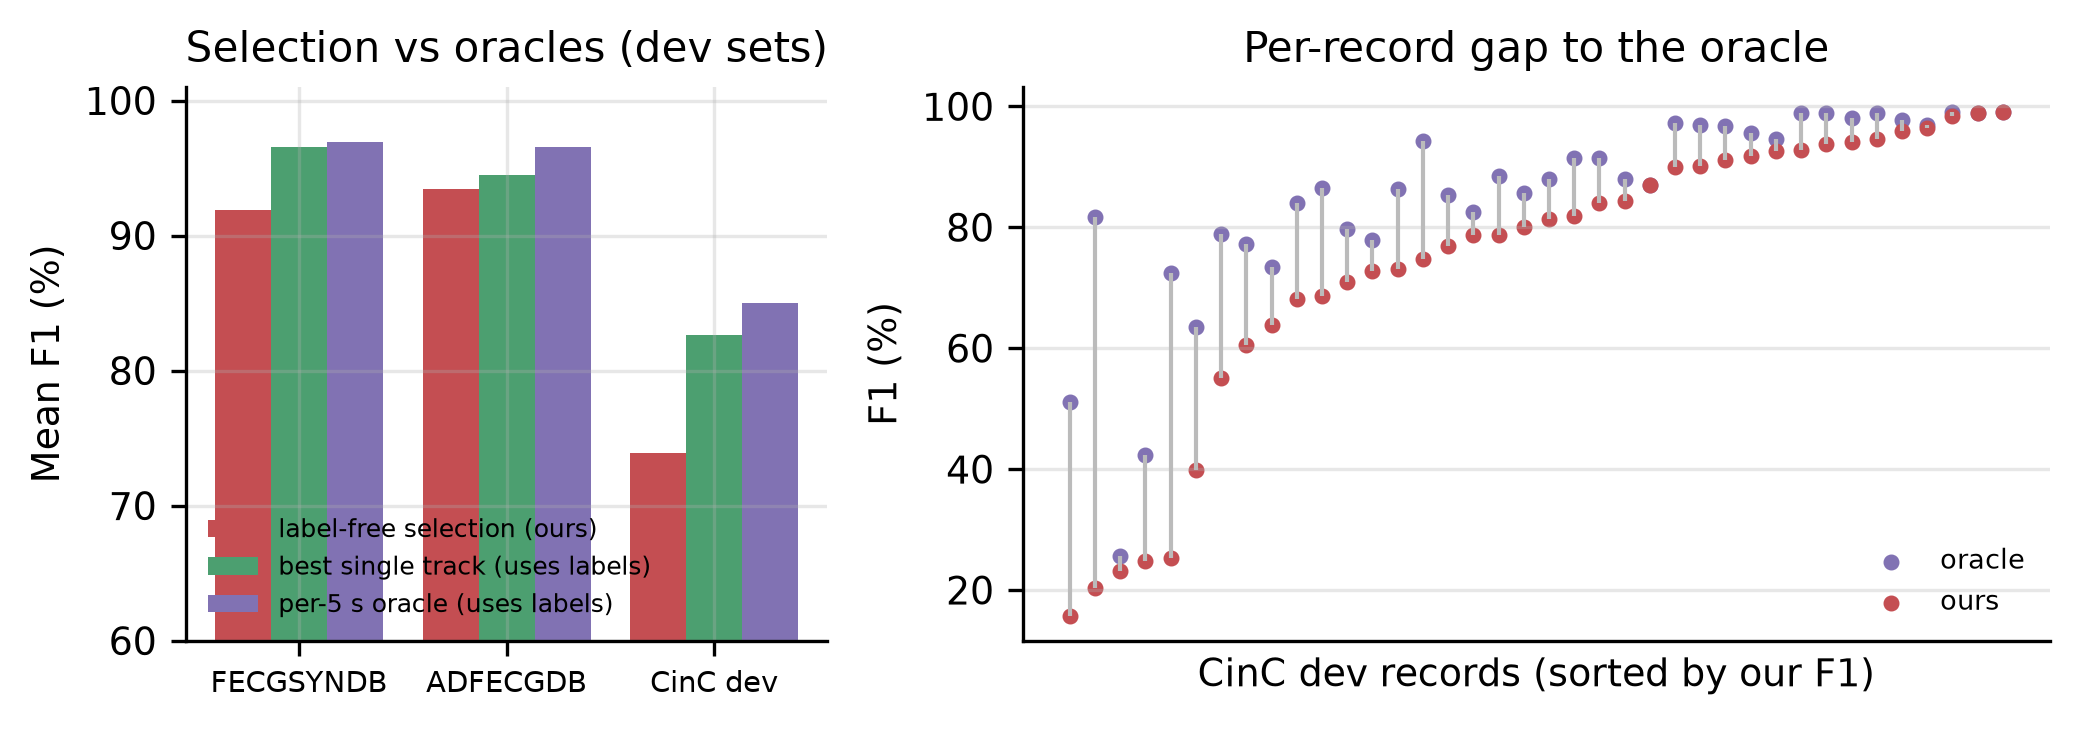
\includegraphics[width=0.92\textwidth]{figures/fin_selection_gap.png}
\caption{\fb Where the remaining real-data error is (diagnostic run on development sets, before the final FHR-prior step; labels used only for this analysis). Left: label-free selection against the best single track and a per-5-s oracle that always picks the right track. Right: per CinC dev record, our selection (red) against the oracle (purple). On CinC dev the selector loses about 9 points to the best track and 11 to the oracle; the candidates themselves are good on most records.}
\label{fig:fin_gap}
\end{figure*}

\begin{figure}[t]
\centering
\fb
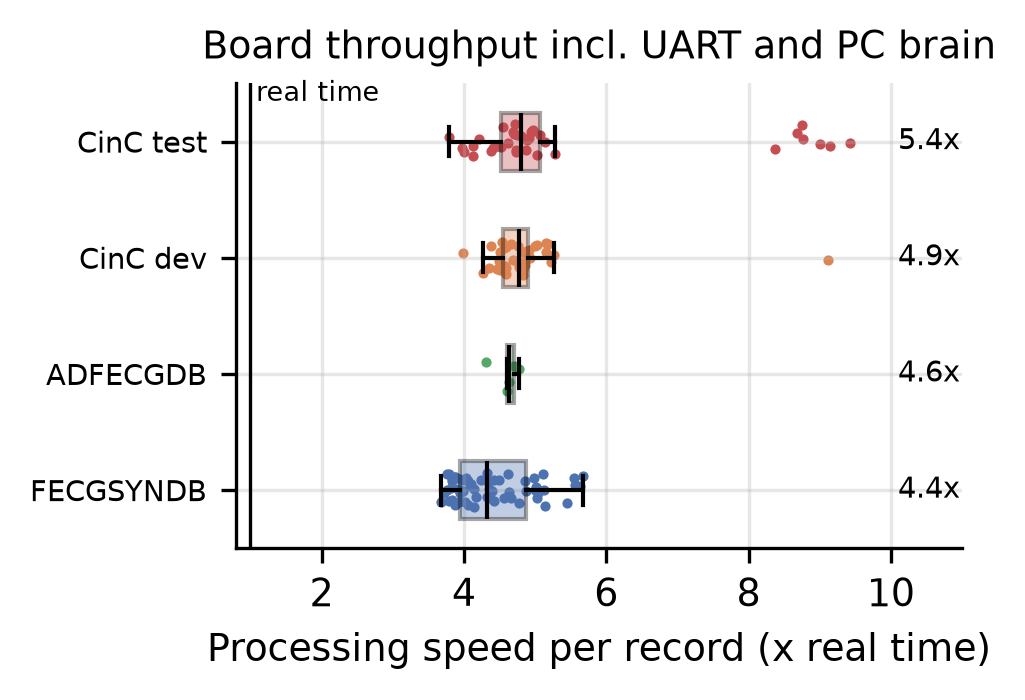
\includegraphics[width=\columnwidth]{figures/fin_board_speed.png}
\caption{\fb Board processing speed per record, including UART transfer and the PC brain (mean of per-record ratios). Every record runs 3.7--9.4$\times$ faster than real time. On CinC a01 (web demonstration log) the median time per 64-sample frame (0.256\,s of signal) was 34\,ms, with a one-off peak of 0.58\,s during calibration.}
\label{fig:fin_speed}
\end{figure}

\noindent\textbf{Summary of the measured results.} On the board, v6 reaches the accuracy of v5 within $\pm 0.8$ points on every set (Tab.~\ref{tab:final_versions}), now without a soft processor. It is bit-exact with the C model on 140 of 140 records (Tab.~\ref{tab:final_results}). It improves held-out real-data F1 from $16.7\%$ (mid-term design, causal) to $65.5\%$, and ADFECGDB from $37.0\%$ (v2) to $92.7\%$, with FHR MAE $2.0\,$bpm on ADFECGDB.

\subsection{Uncertainty of the v6 Numbers}
\label{sec:final_ci}
The test sets are small, so we give 95\% confidence intervals for the mean F1 (bootstrap over records, 10,000 resamples; \cref{tab:final_ci}). The challenge organisers flag the reference annotations of 7 records as inaccurate~\cite{behar2014b}; without them the held-out F1 is $70.4\%$. The intervals of CinC dev and CinC test overlap, which supports the reading that part of the dev/test gap is chance (Sec.~\ref{sec:final_obs}).

\begin{table}[t]
\fb
\caption{\fb Board F1 with 95\% bootstrap confidence intervals (records resampled with replacement).}
\label{tab:final_ci}
\centering
\resizebox{\columnwidth}{!}{%
\begin{tabular}{@{}lccc@{}}
\toprule
\textbf{Data set} & \textbf{Records} & \textbf{Mean F1 [95\% CI] (\%)} & \textbf{Median F1 (\%)} \\
\midrule
FECGSYNDB subset & 60 & 91.8 [88.1, 95.2] & 99.6 \\
ADFECGDB & 5 & 92.7 [88.5, 96.1] & 93.1 \\
CinC dev & 38 & 76.0 [68.5, 82.7] & 84.1 \\
\quad reliable references only & 35 & 77.0 [69.2, 83.7] & 84.4 \\
CinC test (held out) & 37 & 65.5 [55.9, 75.0] & 73.6 \\
\quad reliable references only & 33 & 70.4 [61.2, 79.4] & 78.7 \\
\bottomrule
\end{tabular}%
}
\end{table}

\subsection{Failure Analysis on Real Recordings}
\label{sec:final_fail}
To see why some real recordings fail, we re-ran all 75 CinC records through the C model (bit-exact with the board) and read the maternal R peaks and the output beats from its own output stream. \Cref{fig:fin_fail} compares the median output rate with the median reference rate. 58 of 75 records reach F1 $\ge 50\%$ and their output rate sits on the diagonal. The other 17 fall into three groups:
\begin{itemize}
    \item \textbf{Followed the mother (7 records).} The output rate is in the adult range (82--99\,bpm). In 5 of these the maternal detector never found a regular maternal train, so no maternal cancellation was done and the strongest remaining rhythm was the mother. In a65 the ``maternal'' train it found was at 141.5\,bpm, the fetal rate: it cancelled the fetus and then tracked the mother. In a69 the maternal train was right (90\,bpm), but the selector still chose a track whose beats all coincide with maternal R peaks.
    \item \textbf{Wrong fetal-range track (5 records).} The median output rate is in the fetal range but wrong (e.g.\ a46: 121 against 133\,bpm, a29: 153 against 133\,bpm). The output switches between tracks, some of them noisy or at the maternal rate (a46 in \cref{fig:fin_fail}).
    \item \textbf{Unreliable reference (5 records).} The challenge organisers flag these annotations as inaccurate~\cite{behar2014b} (e.g.\ a54, whose annotations give an implausible flat 100\,bpm after 27\,s), so a low score does not prove a wrong output.
\end{itemize}
The first group points to the most useful improvement. Looking at the detectors showed why no maternal train was found; v6.1 fixes this cause (Sec.~\ref{sec:v61}), and with v7-DL no CinC record is left without a maternal train (Sec.~\ref{sec:v7_where}).

\begin{figure*}[t]
\centering
\fb
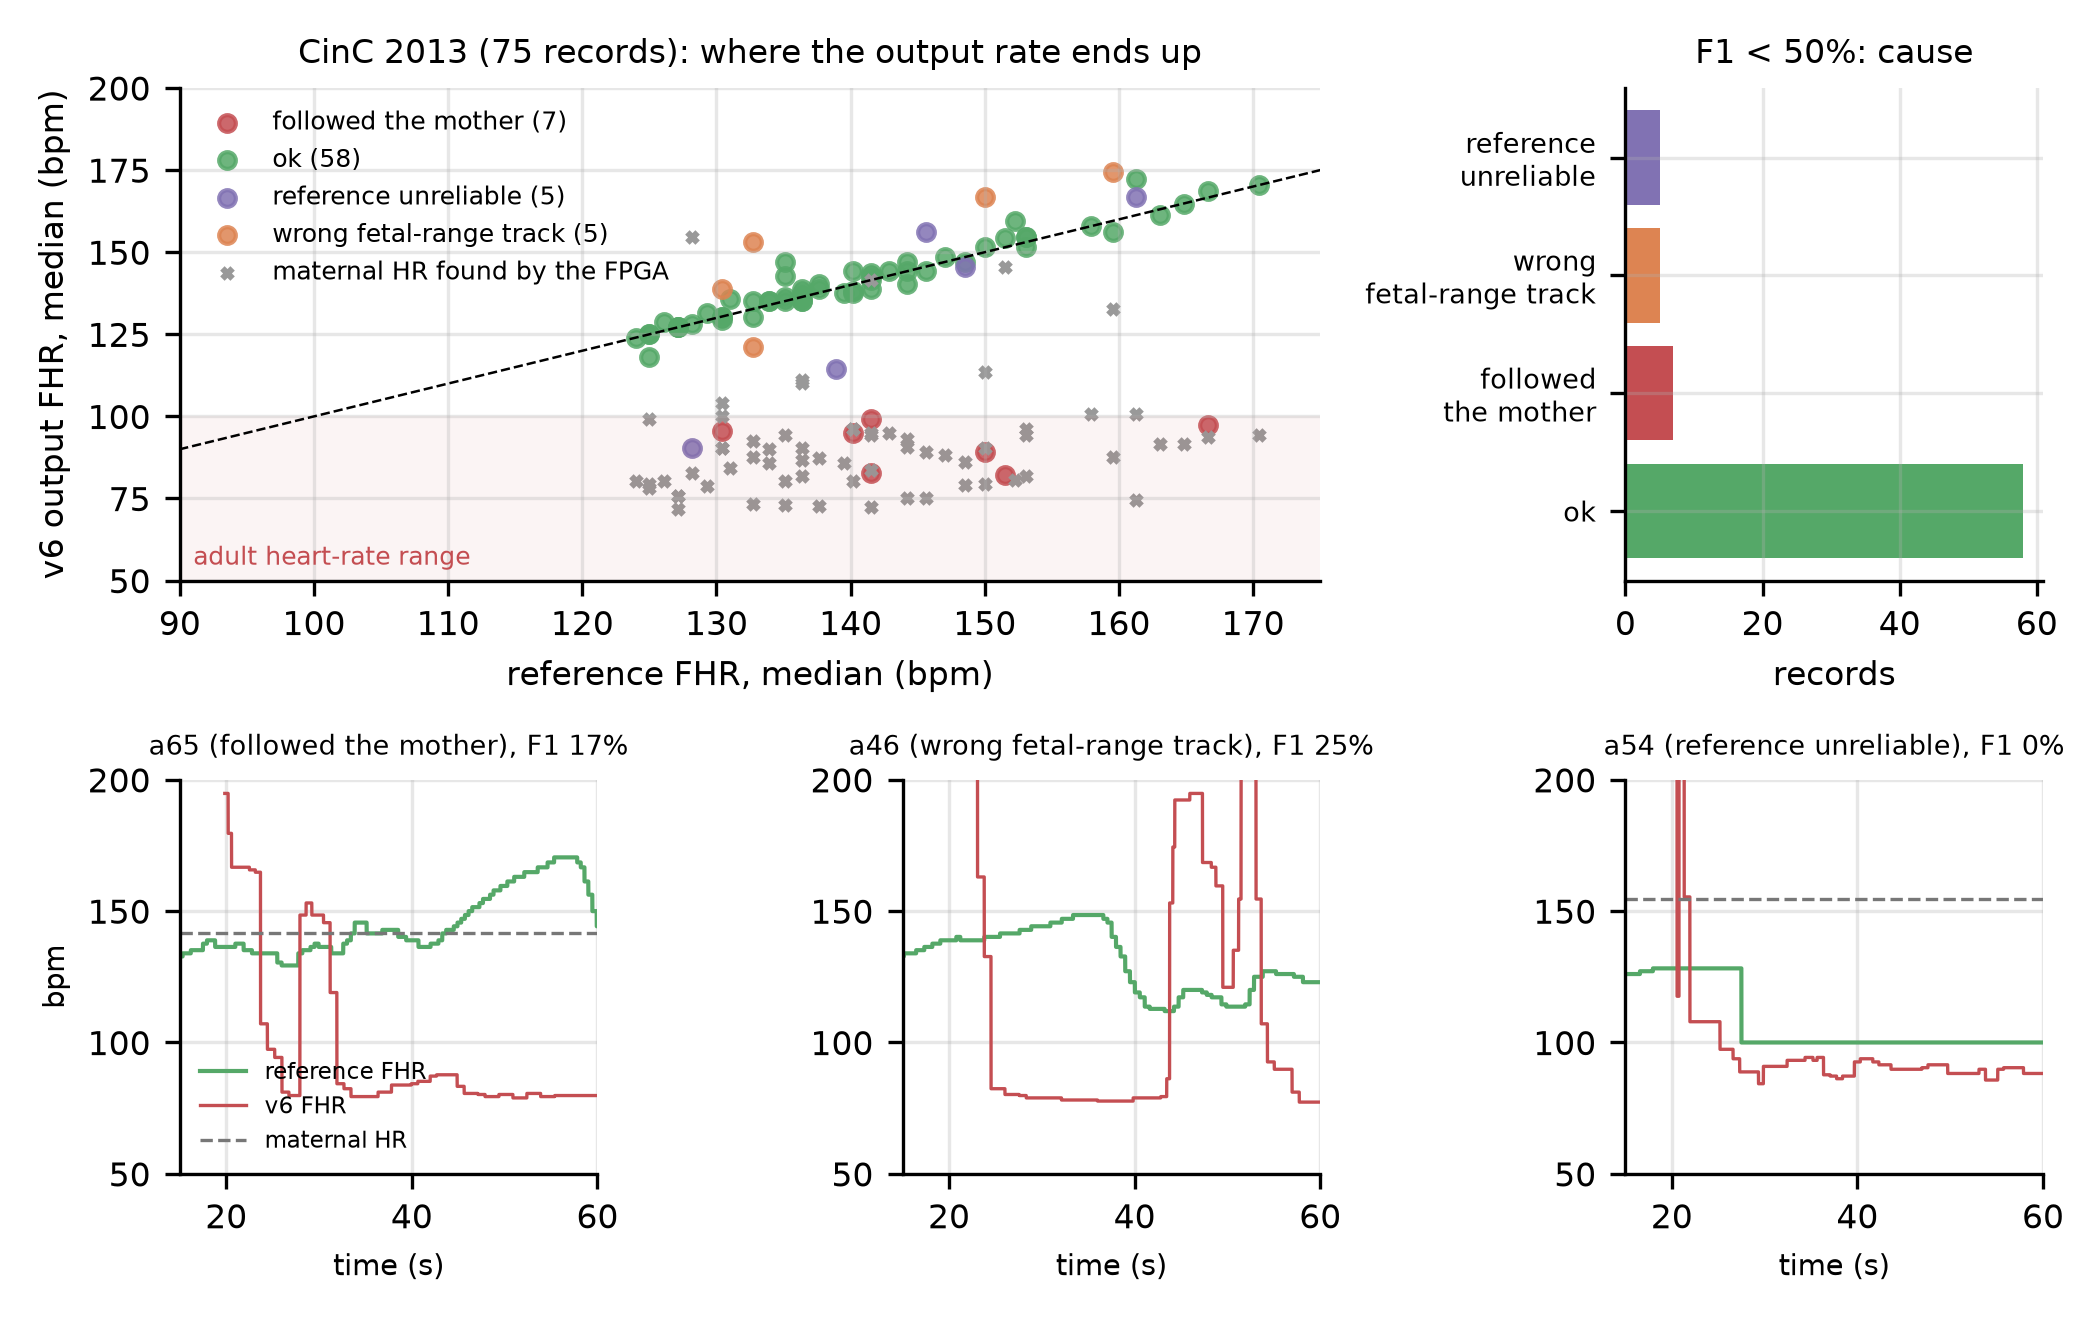
\includegraphics[width=0.92\textwidth]{figures/fin_failures.png}
\caption{\fb Failure analysis on all 75 CinC 2013 recordings (C model, bit-exact with the board). Top left: median output FHR against median reference FHR; grey crosses are the maternal heart rate found by the FPGA (missing where no maternal train was found). Top right: causes for the 17 records with F1 below $50\%$. Bottom: one example per cause, with the reference FHR, the v6 output and the maternal rate.}
\label{fig:fin_fail}
\end{figure*}

% =====================================================================
\renewcommand{\topfraction}{0.5}% keeps deferred floats from filling the columns that hold the [H] figures below
\section{Final Phase IV: Accuracy Improvements and On-Chip Look-Ahead (v6.1, v7)}
\label{sec:final_v7}

The failure analysis and the oracle study of v6 (Sec.~\ref{sec:final_fail}, Fig.~\ref{fig:fin_gap}) pointed to three label-free improvements. We implemented them on the C model first (v6.1) and then built two versions that may use future samples: an offline reference on the PC (v7-LA) and a look-ahead unit inside the FPGA that keeps the recording streamed in small frames (v7-DL, the final design). The rules of Sec.~\ref{sec:final_realdata} still apply: all decisions were made on the development sets, annotations are used only for scoring, and CinC test was scored once per frozen design. CinC test had already been scored for v5 and v6, so it is not a fresh test set for these versions, but no decision used it.

\subsection{v6.1: Three Label-Free Improvements}
\label{sec:v61}
\noindent\textbf{1. Robust maternal detector.} In 4 of the 5 CinC failures where no maternal train was found, all four maternal detectors fired zero times in the whole recording. The detector's peak level was only updated on a detection, so one large start-up transient set a threshold that was never crossed again. v6.1 starts the detector warm-up at sample 256, after the filter transient, and lets the peak level decay by $1/8$ at every sub-threshold local maximum once 2\,s have passed without a detection. In a73 the mother is now found at 96\,bpm, and in a65 the real 81-bpm mother replaces the fetal-rate train.

\noindent\textbf{2. Smarter causal selection (not adopted).} We tried a maternal-rate penalty, rate voting across tracks, an FHR-continuity rule, other window lengths and term weights, and a logistic selector trained on 120 other synthetic records. The best rule gained $+0.5$ on CinC dev but lost 0.6--1.4 points on FECGSYNDB, and the learned selector lost 0.5 on CinC dev (Tab.~\ref{tab:v61_ideas}), so the v6 selector was kept. After idea 1 the causal choice still lost about 5 points to the best single track (CinC dev $79.5$ against $84.7$, FECGSYNDB subset $91.1$ against $96.6$).

\noindent\textbf{3. Periodic recalibration.} Every 30\,s the FPGA sends the latest 12\,s of $\mathbf{z}$ and $\mathbf{x}_f$ again (read back from its sample rings) and asks for new GEVD filters. The PC keeps a track's old filter unless the new one gives a better beat train by a label-free score (regularity $\times$ completeness $\times$ (1 $-$ maternal coincidence)), and the FPGA cross-fades to the new weights over 64 samples. The message protocol is unchanged.

\begin{table}[H]
\fb
\caption{\fb The three ideas on the development sets (C model, mean F1 in \%). Each row adds to the adopted rows above it.}
\label{tab:v61_ideas}
\centering
\resizebox{\columnwidth}{!}{%
\begin{tabular}{@{}lcccl@{}}
\toprule
\textbf{Variant} & \textbf{CinC dev} & \textbf{ADFECGDB} & \textbf{FECGSYNDB sub.} & \textbf{Decision} \\
\midrule
v6 (frozen, = board) & 76.04 & 92.73 & 91.83 & -- \\
1: detector warm-up at 256 + peak decay & 79.52 & 93.31 & 91.11 & adopted \\
2: maternal-rate penalty $\times 0.2$ & 80.04 & 93.31 & 89.72 & rejected \\
2: logistic selector (trained on synthetic) & 78.91 & 93.68 & 90.83 & rejected \\
3: recalibrate every 30\,s, keep if better & \textbf{80.41} & \textbf{92.87} & \textbf{91.64} & adopted (= v6.1) \\
\bottomrule
\end{tabular}%
}
\end{table}

\noindent\textbf{v6.1 in the RTL.} v6.1 is selected with the Verilog define \texttt{V61}. The detector change touches \texttt{v6\_det} and \texttt{v6\_mat}. Recalibration adds ten states to \texttt{v6\_trk} that read 3,000 samples back from the rings, send them as calibration data, request the new weights and restart the cross-fade from the kept weights. The system testbench gives 0 byte errors on 8 records (one of them with three recalibrations); the build meets timing at 50\,MHz (Tab.~\ref{tab:v7_hw}).

\subsection{v7-LA: Offline Look-Ahead on the PC}
\label{sec:v7la}
v7-LA is a non-causal reference that runs on the PC after the recording, still without labels. It takes the v6.1 output stream of the whole recording (the 16 candidate tracks with their beats, beat snapshots and envelope medians, and the maternal R peaks) and:
\begin{enumerate}
    \item scores every track in centred $\pm 15\,$s windows with the quality terms of Sec.~\ref{sec:final_algo} (beat-shape consistency, completeness, RR regularity squared, FHR prior, gated maternal penalty, agreement with the other tracks);
    \item finds the best track path over the whole recording with a Viterbi search on 2.5-s segments, maximising the summed log-quality minus a switching cost of 1, where switching between two tracks that agree on more than 80\% of their beats is free;
    \item cleans up the beats using the rhythm on both sides: it fills one missed beat from the nearest candidate beat and drops a beat that splits an interval;
    \item computes the FHR from a centred median of 5 intervals.
\end{enumerate}
On the development sets the window length and the switching cost changed the result by less than 0.4 points, while the maternal confidence gate was essential (FECGSYNDB subset $78.4\%$ without, $93.8\%$ with). v7-LA scores $75.6\%$ on CinC test ($80.9\%$ on reliable references), $84.6\%$ on CinC dev, $95.8\%$ on ADFECGDB and $94.3\%$ on all 1,248 FECGSYNDB records, with the largest gain on ectopic beats ($c4$: $77.9 \to 85.8\%$).

\subsection{v7-DL: Look-Ahead on the FPGA with a Fixed Delay}
\label{sec:v7dl}
v7-LA needs the whole recording. v7-DL does the same kind of look-ahead on the FPGA as a stream: the PC still sends the recording in 64-sample frames, and the board outputs the final beats with a fixed delay.

\noindent\textbf{The look-ahead unit.} A new RTL unit, \texttt{v7\_la}, only listens to the other units: it taps every word they write to the uplink (beats, beat snapshots, maternal R peaks, the covariance) and two PC answers (maternal PCA vectors and train index). It never changes the v6.1 stream; it only adds frames. Every 2.5\,s of signal (Fig.~\ref{fig:fin_v7_timing}) it
\begin{enumerate}
    \item scores all 16 tracks over a window from 15\,s before to 7.5\,s after the segment with an integer version of the quality in $\log_2$ (Q8). Shape consistency is the norm of the mean of the normalised beat snapshots, so only 31 sums per track and 2.5-s slot are stored. Completeness, regularity, the FHR prior (a table), the maternal penalty with the 10\% energy gate ($10\,\mathbf{v}^T\mathbf{C}\mathbf{v} \ge \text{trace}\,\mathbf{C}$) and the agreement term are counts and ratios;
    \item runs one Viterbi step over the 16 tracks and decides the segment from the best current path;
    \item cleans up the decided beats in one pass, computes the centred FHR and sends each final beat as an OUT7 frame (time, FHR, track). A deadline sends any beat that has waited 15\,s even if its look-ahead beats are missing.
\end{enumerate}
At the end of a recording the PC sends FLUSH; the unit finishes the remaining segments with the data it has and sends END7 with the number of final beats. A second small unit drives the board's two 4-digit displays with the latest final FHR and the number of final beats.

\begin{figure}[H]
\centering
\fb
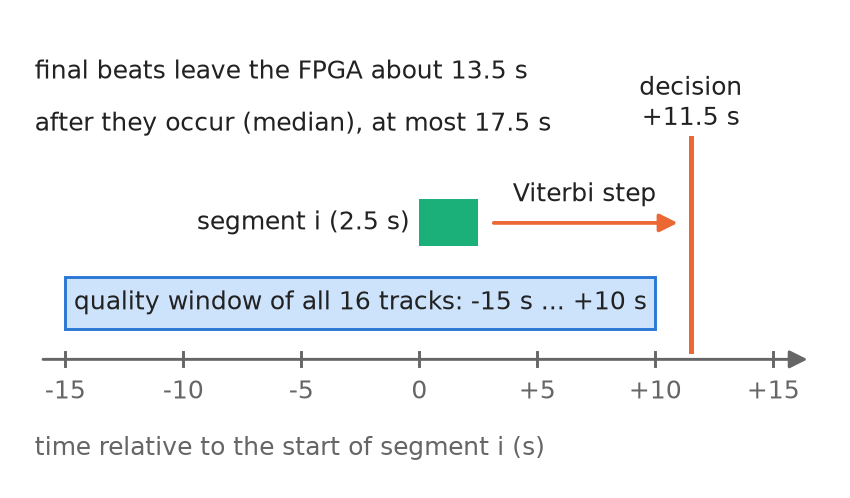
\includegraphics[width=\columnwidth]{figures/fin_v7_timing.png}
\caption{\fb When v7-DL decides a segment. Every 2.5\,s of signal the look-ahead unit scores all 16 tracks over a window from 15\,s before to 7.5\,s after the segment, 1.5\,s after the end of that window so that the beats in it have been reported, runs one Viterbi step and decides the segment. After the clean-up and the centred FHR the final beats leave the FPGA about $13.5\,$s after they occurred (median); a deadline sends any beat that has waited 15\,s, so no beat is later than $17.5\,$s.}
\label{fig:fin_v7_timing}
\end{figure}


\noindent\textbf{Choosing the delay (development sets only).} A future window of three segments, decision lag 0 and one clean-up pass gave CinC dev $84.7\%$, ADFECGDB $96.1\%$ and FECGSYNDB subset $93.4\%$ with a median output delay of $13.5\,$s. A decision lag of one segment and two clean-up passes gained at most $0.2$ points but raised the median delay to $17.9\,$s. The 15-s deadline left every F1 unchanged and caps the delay at $17.5\,$s.

\begin{figure}[H]
\centering
\fb
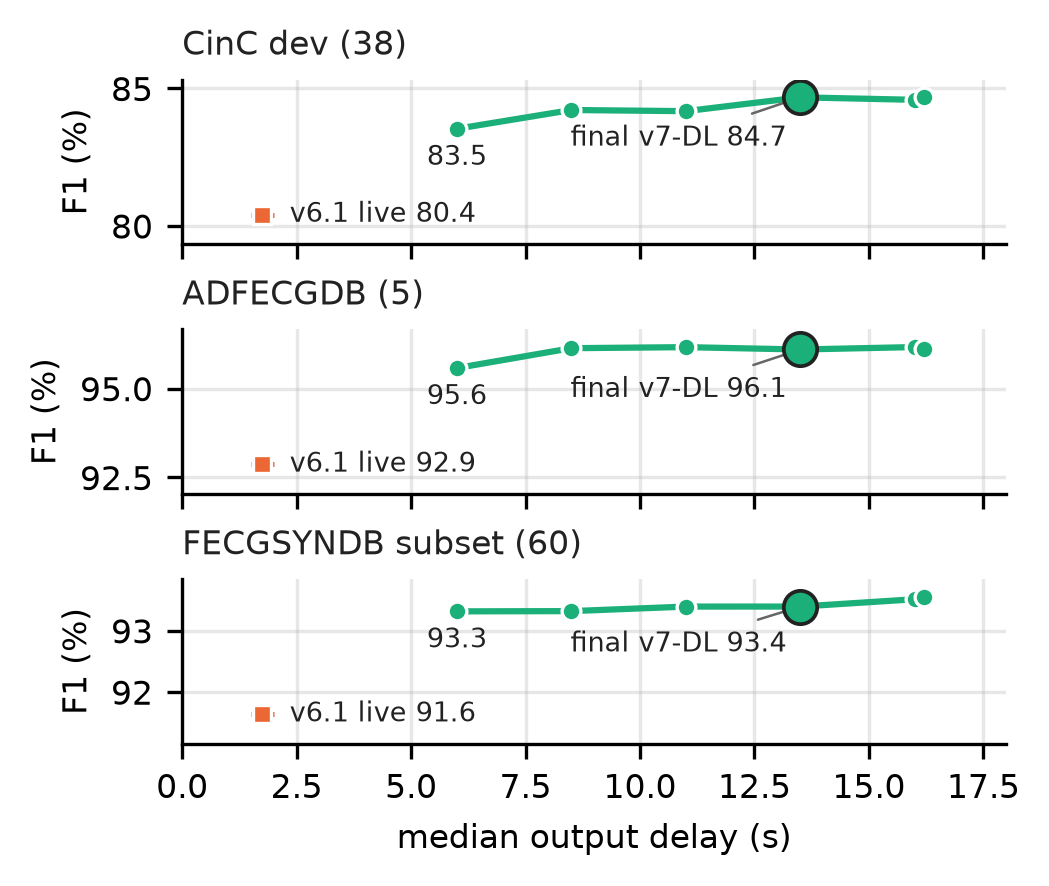
\includegraphics[width=\columnwidth]{figures/fin_v7_delay.png}
\caption{\fb Mean F1 of v7-DL against its median output delay on the development sets (C model, which is bit-exact with the board), for future windows of 0, 1, 2, 3, 4 and 5 segments of 2.5\,s. The large marker is the final design (3 segments, $13.5\,$s); the orange square is the live v6.1 output, whose beats leave 1.5--2\,s after they occur. The y axes differ between panels.}
\label{fig:fin_v7_delay}
\end{figure}

\noindent\textbf{Accuracy against delay.} \Cref{fig:fin_v7_delay} repeats the choice for future windows of 0 to 5 segments (development sets, C model, everything else frozen). Most of the gain needs little future: deciding each segment 1.5\,s after it ends, with no future segments, gives CinC dev $83.5\%$ at a median delay of $6.0\,$s, against $80.4\%$ for the live v6.1 output and $84.7\%$ for the chosen three segments ($13.5\,$s); more than three segments gives nothing. The deadline sets the maximum delay and changed no F1 by more than $0.01$ points: with no future segments and a 5-s deadline no beat leaves later than $8.0\,$s. A monitor that needs a faster final value can therefore trade about one point on CinC dev for half the delay (values in \texttt{tables/v7\_delay\_sweep.csv}).

\noindent\textbf{Verification and area.} As before, an integer C model (\texttt{v7\_post.c}) is the specification. The system testbench, extended with FLUSH, gives 0 byte errors on 9 records (CinC, ADFECGDB and FECGSYNDB). The first RTL version of the unit used 13.2k LUTs on its own and the whole design did not fit (101\% of the LUTs). Doing the shifts, the divisions and the $\log_2$ one bit per cycle and giving the small buffers a single read port cut the unit to 8.4k LUTs with identical output; the unit runs only once per 2.5\,s of signal, so the extra cycles cost nothing. \Cref{tab:v7_hw} compares the three hardware versions.

\begin{table}[H]
\fb
\caption{\fb FPGA utilisation of the three hardware versions on the XC7S50 (Vivado post-implementation, 50\,MHz).}
\label{tab:v7_hw}
\centering
\resizebox{\columnwidth}{!}{%
\begin{tabular}{@{}lccc@{}}
\toprule
\textbf{Resource} & \textbf{v6} & \textbf{v6.1} & \textbf{v7-DL (final)} \\
\midrule
LUTs (of 32,600) & 18,127 (55.6\%) & 18,986 (58.2\%) & \textbf{26,701 (81.9\%)} \\
Flip-flops & 10,015 & 11,179 & \textbf{15,970} \\
DSP48E1 (of 120) & 33 & 33 & \textbf{43} \\
Block RAM tiles (of 75) & 60 & 60 & \textbf{71} \\
Worst slack & +0.26\,ns & +0.41\,ns & \textbf{+0.05\,ns} \\
On-chip power (estimate) & 0.374\,W & 0.386\,W & \textbf{0.445\,W} \\
\bottomrule
\end{tabular}%
}
\end{table}

\subsection{Results of v6.1 and v7-DL on the Board}
\label{sec:v7_results}
Both versions were run on the Spartan-7 on the same 140 records as v6, and the complete output stream of every record was compared with the C model: 140/140 records bit-exact for v6.1 and for v7-DL. For v7-DL the board sends both outputs in the same run: the live v6.1 beats and, about 13.5\,s later, the final look-ahead beats. \Cref{tab:v7_results} and \cref{fig:fin_v7_results} give the results; the board runs 4.0--4.5$\times$ faster than real time for both versions.

\begin{figure}[H]
\centering
\fb
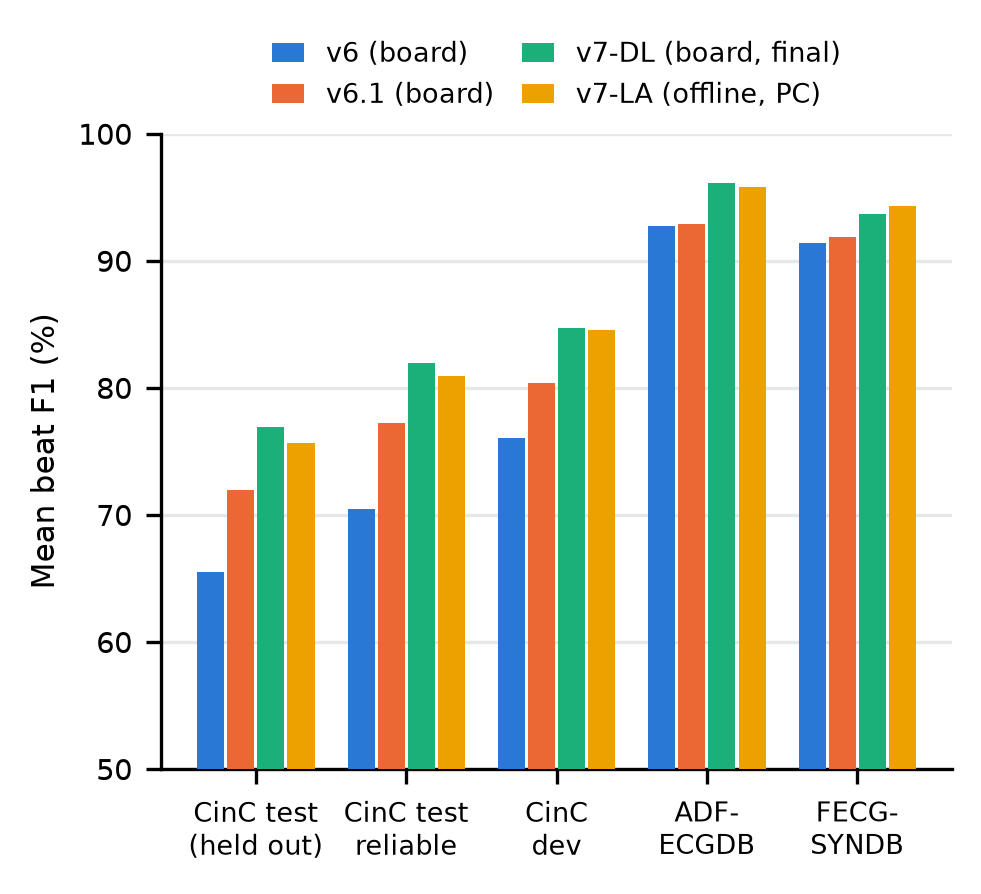
\includegraphics[width=\columnwidth]{figures/fin_v7_results.png}
\caption{\fb Mean F1 of v6, v6.1 and v7-DL measured on the board and of the offline v7-LA (PC, whole recording) on every data set. v7-DL, which runs on the FPGA with a fixed delay, is at least as good as the offline version on all real data sets and within 0.7 points on FECGSYNDB.}
\label{fig:fin_v7_results}
\end{figure}

\begin{table}[H]
\fb
\caption{\fb v6.1 and v7-DL on the board (every record bit-exact with the C model): mean F1 with 95\% bootstrap confidence intervals (records resampled 10,000 times) and FHR MAE. \emph{Reliable refs}: without the 7 flagged records~\cite{behar2014b}. The last row is the C model on all FECGSYNDB records.}
\label{tab:v7_results}
\centering
\resizebox{\columnwidth}{!}{%
\begin{tabular}{@{}lcccc@{}}
\toprule
\textbf{Data set} & \textbf{Rec.} & \textbf{v6.1 F1 (\%)} & \textbf{v7-DL F1 (\%)} & \textbf{FHR MAE (bpm)} \\
 & & \textbf{[95\% CI]} & \textbf{[95\% CI]} & \textbf{v6.1 / v7-DL} \\
\midrule
FECGSYNDB subset & 60 & 91.6 [87.3, 95.4] & 93.4 [89.3, 96.7] & 5.36 / 4.23 \\
ADFECGDB & 5 & 92.9 [88.6, 96.3] & 96.1 [92.8, 98.9] & 1.72 / 2.13 \\
CinC dev & 38 & 80.4 [73.9, 85.8] & 84.7 [78.6, 89.8] & 8.91 / 6.45 \\
\quad reliable refs & 35 & 81.6 [75.0, 87.1] & 86.0 [79.9, 90.8] & 8.25 / 6.09 \\
\textbf{CinC test} & \textbf{37} & \textbf{71.9 [63.2, 80.2]} & \textbf{76.9 [68.3, 84.7]} & \textbf{11.16 / 11.53} \\
\quad reliable refs & 33 & 77.2 [69.5, 84.2] & 82.0 [74.7, 88.5] & 9.44 / 10.44 \\
CinC all & 75 & 76.2 [70.7, 81.4] & 80.8 [75.5, 85.7] & 10.02 / 8.96 \\
\quad reliable refs & 68 & 79.5 [74.3, 84.1] & 84.0 [79.2, 88.3] & 8.83 / 8.20 \\
\midrule
FECGSYNDB all & 1,248 & 91.9 & 93.7 & 4.85 / 3.98 \\
\bottomrule
\end{tabular}%
}
\end{table}


On held-out CinC, v7-DL improves 33 records and worsens 1 by more than one point compared with the live v6.1 output of the same runs (Fig.~\ref{fig:fin_v7_cinc}), and 18 records reach $\ge 90\%$ (v6.1: 15, v6: 13). Without the 7 records with inaccurate references, v7-DL scores $86.0\%$ on CinC dev, $82.0\%$ on CinC test and $84.0\%$ on the remaining 68 CinC records ($80.8\%$ on all 75). The 7 records come from the organisers' list, not from our results: 5 of them are among our failures, and the other two score $92.5\%$ and $79.6\%$. The sensitivity of v7-DL and PPV on CinC test are $76.2\%$ and $77.8\%$, and on ADFECGDB $96.4\%$ and $95.8\%$. Its FHR error is lower than that of v6.1 on CinC dev and FECGSYNDB, but slightly higher on CinC test (11.5 against 11.2\,bpm) and ADFECGDB (2.1 against 1.7\,bpm). Through the web page (Sec.~\ref{sec:final_demo}) CinC a01 gave the same 102 final beats as the C model (F1 $98.0\%$; live v6.1 output $95.1\%$).

\begin{figure}[H]
\centering
\fb
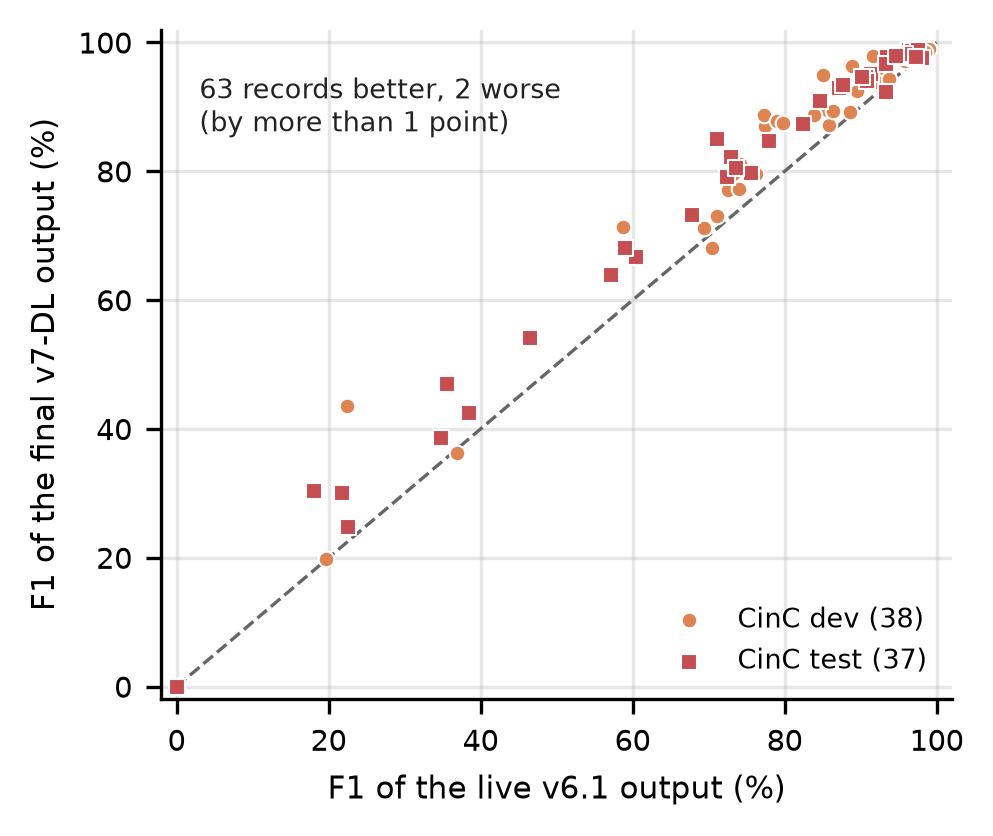
\includegraphics[width=\columnwidth]{figures/fin_v7_cinc.png}
\caption{\fb Per-record F1 of the final v7-DL output against the live v6.1 output of the same board runs on all 75 CinC recordings: 63 records improve by more than one point and 2 get worse.}
\label{fig:fin_v7_cinc}
\end{figure}


\subsection{Where the Remaining Error Is}
\label{sec:v7_where}
We repeated the oracle diagnostic with v7-DL on all 75 CinC records (labels used only for this analysis). The final output scores $80.8\%$ on average against $82.1\%$ for the best single candidate track, so with look-ahead the choice of track is no longer the main loss. Of the 15 records below $70\%$:
\begin{itemize}
    \item 5 have references that the challenge organisers flag as inaccurate (a38, a52, a54, a71, a74); the other two flagged records, a33 and a47, score $92.5\%$ and $79.6\%$;
    \item 8 have no candidate track above $70\%$ (best track 42--69\%): the fetal beats are not recovered by any of the 16 spatial filters;
    \item 2 have a best track of 71--73\%;
    \item none has a good track ($\ge 85\%$) that was not chosen, and the maternal train is found in all 75 records.
\end{itemize}
The next real-data gain must therefore come from better candidates, i.e.\ from the front end and the spatial filters, not from the selection. On FECGSYNDB the weakest condition stays ectopic beats ($c4$, about $84\%$ at every SNR, Fig.~\ref{fig:fin_v7_cond}): the regularity term and the clean-up treat an early beat and the following pause as errors.

\begin{figure}[H]
\centering
\fb
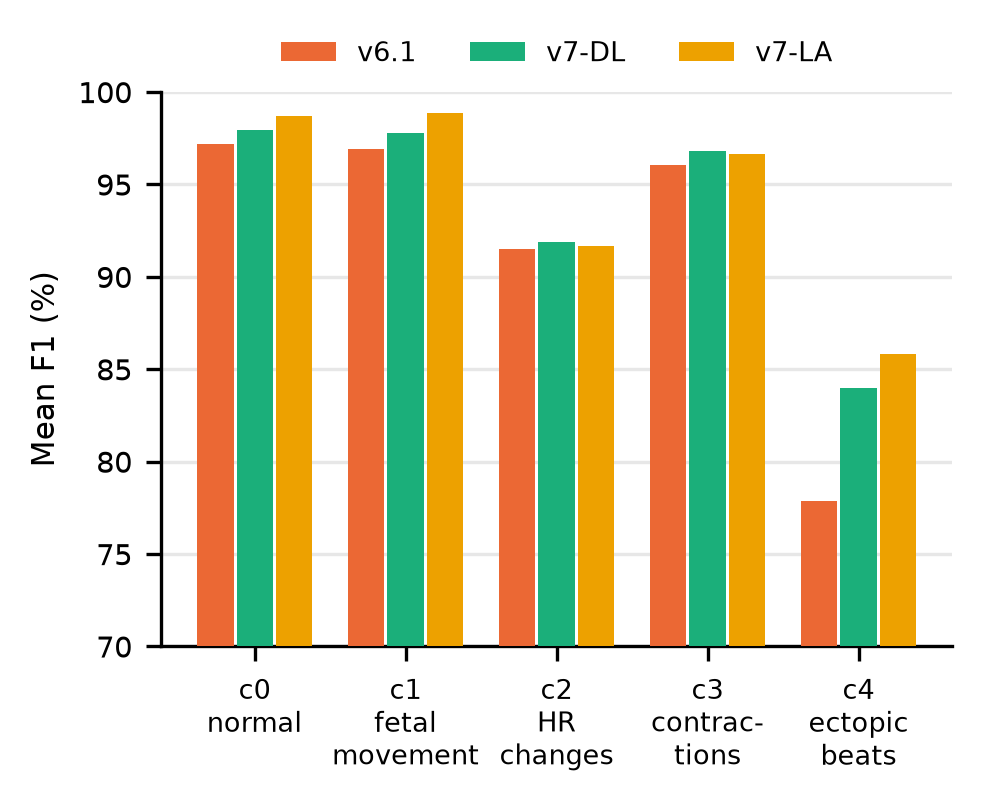
\includegraphics[width=\columnwidth]{figures/fin_v7_conditions.png}
\caption{\fb FECGSYNDB (1,248 records, C model) by condition; v7-DL: $c0$ 98.0, $c1$ 97.8, $c2$ 91.9, $c3$ 96.8, $c4$ 84.0. The look-ahead helps most on ectopic beats ($c4$), which nevertheless stay the weakest condition.}
\label{fig:fin_v7_cond}
\end{figure}

\subsection{Comparison with Published Results}
\label{sec:v7_literature}
\Cref{tab:v7_literature} places the final design next to published fetal QRS detectors on the same three data sets. All numbers are beat F1 with a $\pm 50\,$ms tolerance. The comparison is not like for like:
\begin{itemize}
    \item the published methods are not causal (for example zero-phase filtering in~\cite{behar2014b} and backward Kalman smoothing in~\cite{andreotti2014}), several were developed on set-a and scored on the same records, and they score almost the whole minute. v7-DL runs on the FPGA with a fixed $13.5\,$s delay, was never tuned on CinC test and is scored from $20\,$s;
    \item the FECGSYNDB results of~\cite{andreotti2016} are medians, so we give our median too (our mean is $93.7\%$).
\end{itemize}
Published results on set-a range from $61.6\%$ to $97.3\%$. On real data v7-DL ($84.0\%$) is at the level of the classic template-subtraction methods and about 10 points below the best offline methods; on ADFECGDB and FECGSYNDB it is within the published range.

\begin{table}[t]
\fb
\caption{\fb Final design against published fetal QRS detection results (beat F1 in \%, $\pm 50\,$ms). Published methods run offline; v7-DL runs on the FPGA with a fixed delay. Rec.: records scored (--: not stated). $^a$5 records excluded, parameters tuned on set-a. $^b$Median F1.}
\label{tab:v7_literature}
\centering
\resizebox{\columnwidth}{!}{%
\begin{tabular}{@{}lcc@{}}
\toprule
\textbf{Method} & \textbf{Rec.} & \textbf{F1 (\%)} \\
\midrule
\multicolumn{3}{@{}l}{\textit{CinC 2013 set-a (real, 4 abdominal leads)}} \\
QRStree~\cite{zhong2019} & 68 & 61.6 \\
TS / TSpca, Behar \etal~\cite{behar2014b} & 68 & 81.6 / 86.1 \\
TSpca-ICA / fusion, Behar \etal~\cite{behar2014b} & 68 & 93.0 / 96.0 \\
Power-MF~\cite{jaeger2024}$^a$ & 70 & 94.3 \\
SCTD-ICA, one lead~\cite{asadi2026} & -- & 95.8 \\
Template adaptation, Andreotti \etal~\cite{andreotti2014} & 74 & 97.3 \\
\textbf{v7-DL (ours, board)} & \textbf{68} & \textbf{84.0} \\
\quad held-out half only & 33 & 82.0 \\
\midrule
\multicolumn{3}{@{}l}{\textit{ADFECGDB (real, scalp-electrode reference)}} \\
QRStree~\cite{zhong2019} & 5 & 95.5 \\
SCTD-ICA, one lead~\cite{asadi2026} & -- & 96.1 \\
DPSS, one lead~\cite{shokouhmand2023} & -- & 97.7 \\
\textbf{v7-DL (ours, board)} & \textbf{5} & \textbf{96.1} \\
\midrule
\multicolumn{3}{@{}l}{\textit{FECGSYNDB (synthetic)}} \\
Best BSS / TS / adaptive, Andreotti \etal~\cite{andreotti2016}$^b$ & -- & 99.9 / 96.0 / 97.9 \\
\quad ectopic beats$^b$ & -- & 83.4--88.4 \\
DPSS, one lead~\cite{shokouhmand2023} & -- & 99.0 \\
\textbf{v7-DL (ours, C model)}$^b$ & \textbf{1,248} & \textbf{99.8} \\
\quad ectopic beats ($c4$)$^b$ & 250 & 89.3 \\
\bottomrule
\end{tabular}%
}
\end{table}


% =====================================================================
\section{Observations and Discussion}
\label{sec:final_obs}

\begin{enumerate}
    \item \textbf{Synthetic results overstate real accuracy.} The mid-term design scored $93.0\%$ on FECGSYNDB in batch mode but $82.2\%$ causally and $16.7\%$ on real held-out recordings. The U-Net and v2 both drop by 60--70 points from synthetic to real (Fig.~\ref{fig:fin_synreal}). A design must be judged on real recordings with a held-out split.
    \item \textbf{A single spatial filter is not enough on real data.} Even with perfect (label-based) weights, one 4-lead linear filter reaches only $60\%$ on CinC. The largest gains came from removing the maternal ECG beat by beat before spatial filtering and from keeping several candidate tracks instead of committing to one filter.
    \item \textbf{Causal selection was the main error of v6; look-ahead closed most of it.} For v6 on CinC dev the best single candidate track scored $82.6\%$ and a per-window oracle $85.0\%$, against about $75\%$ for the causal label-free choice (Fig.~\ref{fig:fin_gap}). Better causal rules did not close this gap (Tab.~\ref{tab:v61_ideas}). Letting the selector see 7.5\,s of the future did: on all 75 CinC records v7-DL scores $80.8\%$ against $82.1\%$ for the best single track (Sec.~\ref{sec:v7_where}).
    \item \textbf{Real-data gains cost some synthetic accuracy.} FECGSYNDB dropped from $95.6\%$ (v2) to $91.4\%$. On some synthetic records the maternal detector locks onto the fetus; the $10\%$ energy confidence gate recovers most of this ($78.7 \to 91.3$ on the subset) without hurting real data. We gave real data priority.
    \item \textbf{Ectopic beats and rate changes remain hard.} The RR-regularity and FHR-prior terms that make selection robust on noisy real data also penalise true irregular fetal rhythms ($c4$: $78.5\%$). The FHR prior also means that fetal bradycardia below about 110\,bpm can be under-selected; we kept the prior mild for this reason (a stronger prior scored $+0.4$ on CinC dev and was rejected).
    \item \textbf{Accuracy grows during a recording.} No beat is output before about $19.5\,$s, and the selector judges tracks over the trailing $20\,$s, so its decisions improve once a full window of data is available. In the web demonstration the running F1 rises over the first tens of seconds. Recalibrating the spatial filters every 30\,s (v6.1) helps mostly on the 5-min recordings; a 60-s CinC record gets at most one recalibration.
    \item \textbf{Dev/test gap.} CinC dev $76.0\%$ against CinC test $65.5\%$. Part is natural variation between the two halves (the dev half was already easier for v2: $42.0$ vs $41.2$ and for the mid-term design: $22.8$ vs $16.7$), part is the effect of choosing the design on the dev half. The test half was never used for a decision; v7-DL shows the same gap ($84.7\%$ against $76.9\%$). The test half has now been scored once for each of v5, v6, v6.1, v7-LA and v7-DL, so it is no longer a fresh test set.
    \item \textbf{A bit-exact model makes hardware debugging tractable.} Writing the integer C model first, comparing every output byte in simulation and on the board, and changing the model before the RTL meant that every bug showed up as the first differing byte. The final RTL has the same output as the model on every record we ran, so the accuracy measured in software is the accuracy of the hardware.
    \item \textbf{Hardware trade-off.} The final design uses about $5\times$ the LUTs of the MicroBlaze version, but it is our own datapath, runs at 50\,MHz with timing met, and is 4--5$\times$ faster than real time. In simulation the RTL alone needs a median of 1,485 cycles per sample, about $140\times$ faster than real time (Fig.~\ref{fig:wave_cycles}); the 4--5$\times$ on the board is set by the UART transfers and the PC answers, not by the FPGA logic. The mid-term resource target ($<5\%$ LUT, 1 DSP) was set for the much simpler beamformer and no longer applies. The look-ahead and display units of v7-DL add 7.7k LUTs and 11 BRAM tiles to v6.1 (82\% of the LUTs in total).
    \item \textbf{Latency against accuracy.} v6 and v6.1 report each beat about $1.5$--$2\,$s after it occurs. v7-DL reports the final beats about $13.5\,$s later (at most $17.5\,$s) and gains 5 points on held-out CinC. The board sends both streams, so a monitor can show the live value at once and replace it with the final one. Neither is suitable for beat-synchronous triggering.
    \item \textbf{The remaining real-data error is in the candidates.} Of the 15 CinC records below $70\%$ with v7-DL, 5 have references the challenge organisers flag as inaccurate and 8 have no candidate track above $70\%$; in none was a good track available but not chosen (Sec.~\ref{sec:v7_where}).
    \item \textbf{On-chip look-ahead needs area-aware RTL.} The first RTL of the look-ahead unit used 13.2k LUTs on its own and the design did not fit. Because the unit runs only once per 2.5\,s of signal, doing its arithmetic one bit per cycle cut it to 8.4k LUTs with identical output; at 82\% LUT use the design still meets timing at 50\,MHz, with little margin ($+0.05\,$ns).
\end{enumerate}
\end{finalpart}

% =====================================================================
\section{Extended Literature Survey and Taxonomic Positioning}
\label{sec:literature_survey}

Published NIFECG extraction literature spans six major algorithmic and implementation paradigms:
\begin{enumerate}
    \item \textbf{Linear Adaptive Filtering (LMS/RLS):} Widrow \etal~\cite{widrow1975} established adaptive noise cancelling (ANC), showing that without a pure maternal reference, single-lead LMS distorts fetal morphology.
    \item \textbf{Subspace Decomposition (SVD/Hankel):} Kanjilal \etal~\cite{kanjilal1997} and Callaerts \etal~\cite{callaerts1990} applied SVD to Hankel trajectory matrices. While effective on clean cycles, Hankel SVD requires high DSP overhead and degrades during QRS collisions.
    \item \textbf{Blind Source Separation (ICA/BSS):} De Lathauwer \etal~\cite{delathauwer2000}, Cardoso~\cite{cardoso1999}, and Hyv{\"a}rinen~\cite{hyvarinen2000} explored ICA. While statistically powerful, iterative ICA algorithms exhibit convergence latency incompatible with real-time FPGA execution.
    \item \textbf{Nonlinear Bayesian Filtering:} Sameni \etal~\cite{sameni2007} developed nonlinear Bayesian filtering frameworks for ECG denoising, demonstrating high noise suppression at the expense of computational complexity.
    \item \textbf{Deep Learning (CNN/U-Net):} Ronneberger \etal~\cite{ronneberger2015} demonstrated biomedical segmentation networks that can be adapted to 1D ECG. However, 1D U-Net requires millions of MACs and exceeds on-chip BRAM capacity.
    \item \textbf{Hardware and Embedded Implementations:} Edwin Dhas and Suchetha~\cite{edwin2022} implemented neural coprocessor adaptive filters on FPGA for fetal ECG extraction. Pani \etal~\cite{pani2016} investigated real-time embedded JADE for fetal ECG. Our architecture builds upon De Lathauwer~\cite{delathauwer2000} and Sameni~\cite{sameni2010}, delivering deterministic single-DSP edge execution.
\end{enumerate}

% =====================================================================
\section{Results Replicated from the Literature}
\label{sec:replications}

In compliance with the EE2000 course guidelines, we independently re-implemented and evaluated key published algorithms. Each replication was built directly from mathematical descriptions without third-party source code. Table~\ref{tab:replication_scorecard} presents our replication scorecard across 7 published literature algorithms.

\begin{table*}[t]
\caption{\tagLone/\tagLtwo\ Comprehensive Literature Replication Scorecard comparing published baselines against our in-house implementations evaluated under identical PhysioNet FECGSYNDB conditions.}
\label{tab:replication_scorecard}
\centering
\resizebox{\textwidth}{!}{%
\begin{tabular}{@{}lp{2.4cm}p{3.2cm}p{3.2cm}p{2.2cm}p{3.6cm}@{}}
\toprule
\textbf{ID} & \textbf{Target Literature Study} & \textbf{Original Published Setup} & \textbf{In-House Setup on FECGSYNDB} & \textbf{Our Obtained Metric} & \textbf{Defensible Scientific Verdict} \\
\midrule
\textbf{R1} & Ahlstrom \etal~\cite{ahlstrom1985} & 4th-order Butterworth bandpass (0.5--40\,Hz) & 4 cascaded SOS at $f_s = 250\,$Hz; causal Direct-Form II & $>56\,$dB at 0.1\,Hz, $>18\,$dB at 60\,Hz & \textbf{Implementation Verified} (exact transfer function matches Fig.~\ref{fig:filter_responses}) \\
\textbf{R2} & Kanjilal \etal~\cite{kanjilal1997} & Hankel SVD rank-2 truncation on single abdominal lead & Hankel matrix $\mathbf{A} \in \mathbb{R}^{m \times (N-m+1)}$, rank-2 subtraction & TC1 F1 = 76.36\%, collapses to 23.72\% on TC3 & \textbf{Trend Replicated on Synthetic Benchmark} (suppresses maternal on clean cycles, collapses during QRS collision) \\
\textbf{R3} & De Lathauwer \etal~\cite{delathauwer2000} & Blind subspace separation on cutaneous abdominal leads & 4-channel spatial covariance eigen-decomposition on suprapubic leads & Fetal dipole isolated in $\mathbf{v}_2$ (7.8\% energy, mat. 88.4\%) & \textbf{Subspace Principle Verified \& Extended} (4-channel spatial projection reduces maternal energy without fetal cancellation) \\
\textbf{R4} & Widrow \etal~\cite{widrow1975} / Hasan~\cite{hasan2009} & Single-lead LMS adaptive filtering without reference & 32-tap transversal LMS on single abdominal channel & TC1 F1 = 15.06\%, FHR MAE = 46.6\,bpm & \textbf{Failure Mechanism Replicated} (confirms maternal residual and fetal distortion when abdominal maternal morphology lacks a dedicated reference lead) \\
\textbf{R5} & Andreotti \etal~\cite{andreotti2016} & Template Subtraction on FECGSYNDB; reported $\approx 78\%$ at 12\,dB, $<35\%$ at 0\,dB & Fixed template subtraction on Lead 27 across TC1--TC3 & TC1 F1 = 76.36\%, dropping to 23.88\% at 0\,dB & \textbf{Matched Benchmark Partially Replicated} (confirms reported performance and severe low-SNR degradation on matched synthetic conditions) \\
\textbf{R6} & Ronneberger \etal~\cite{ronneberger2015} & 2D U-Net biomedical segmentation adapted to 1D ECG & Multi-scale 1D U-Net evaluated on untouched test subjects \texttt{sub09}--\texttt{sub10} & Test F1: 83.93\% (1-Ch), 97.48\% (4-Ch), pop mean 90.76\% & \textbf{Architectural Paradigm Adapted to 1D} (evaluated on two held-out test subjects, $n=2$; high test score contrasted by training underfitting) \\
\textbf{R7} & Widrow \etal~\cite{widrow1975} & Multi-channel ANC using thoracic maternal reference lead & 32-tap NLMS using Lead 32 (0-based thoracic reference) & Literature reported: $\approx 81.2\%$ (12\,dB), $\approx 42.1\%$ (0\,dB) & \textbf{Baseline Explored from Literature} (effective when chest reference exists, but requires extra hardware lead) \\
\bottomrule
\end{tabular}%
}
\end{table*}

% =====================================================================
\begin{finalpart}
\section{Final Demonstration: Live Web Page and On-Board Display}
\label{sec:final_demo}
For the final demonstration the FHR is shown on a local web page and, with v7-DL, also on the board's 7-segment displays planned at mid-term. A small Python server (\texttt{fpga\_implementation/webdemo/}) runs on the laptop connected to the board:
\begin{enumerate}
    \item \textbf{Board check.} The page shows whether the FPGA is connected and answering (a reset plus one empty frame must be acknowledged within 1\,s). If the board does not answer, the page refuses to run; there is no software fallback, so every number shown comes from the hardware.
    \item \textbf{Upload.} Any recording in PhysioNet WFDB format (\texttt{.hea}/\texttt{.dat}, optional annotation file) or a 4-column CSV. Lead units are converted and other sampling rates are decimated causally to 250\,Hz.
    \item \textbf{Real-time playback.} The recording is streamed to the board at its true speed (one 64-sample frame every 0.256\,s) while the PC brain answers the FPGA's requests.
    \item \textbf{Live display.} 10\,s of the four leads with fetal and maternal beat marks, the current FHR and maternal heart rate, the processing stage (filtering, maternal PCA, GEVD calibration, cancellation, tracking), the selected track, the FPGA time per frame and, if annotations exist, the running Se, PPV, F1 and FHR error.
    \item \textbf{Saved output.} Beats (sample, time, FHR, track) and a summary are written to \texttt{webdemo/runs/}.
    \item \textbf{Final and live output (v7-DL).} With the v7-DL bitstream the page shows the final FHR from the look-ahead unit, the live v6.1 estimate under it, the current look-ahead delay, and a signal window that follows the final beats; the heart-rate trend shows the final and the live curve and the part that is not final yet. At the end of the recording the server sends FLUSH and the board finishes the last segment.
    \item \textbf{On-board display.} The v7-DL bitstream also shows the latest final FHR and the number of final beats on the board's two 4-digit seven-segment displays, so the answer is visible on the FPGA board itself.
\end{enumerate}
Run through the page, CinC record a01 gave F1 $95.05\%$, 101 beats and FHR MAE $3.51\,$bpm with v6, identical to the batch board evaluation of the same record, and F1 $98.0\%$ with 102 final beats with v7-DL, identical to the C model.
\end{finalpart}

% =====================================================================
\section{Scope, Limitations, and Validation Status}
\label{sec:limitations}

\begin{finalpart}
\noindent\textbf{Final validation status.} All five validation levels are complete for v6, v6.1 and the final design v7-DL (Tab.~\ref{tab:final_status}).

\begin{table}[t]
\fb
\caption{\fb Validation status of the hardware versions v6, v6.1 and v7-DL (final).}
\label{tab:final_status}
\centering
\resizebox{\columnwidth}{!}{%
\begin{tabular}{@{}llcl@{}}
\toprule
\textbf{Level} & \textbf{Description} & \textbf{Final Status} & \textbf{Evidence} \\
\midrule
\textbf{L1} & Software (causal) & \textbf{Completed} & 1,248 FECGSYNDB + 75 CinC + 5 ADFECGDB records \\
\textbf{L2} & Bit-true model & \textbf{Completed} & Integer C models of v6, v6.1, v7-DL + PC brain \\
\textbf{L3} & RTL simulation & \textbf{Completed} & xsim system test, 8--9 records per version, 0 byte errors \\
\textbf{L4} & Synthesis and timing & \textbf{Completed} & Vivado, 50\,MHz; slack $+0.26$ / $+0.41$ / $+0.05\,$ns \\
\textbf{L5} & Board & \textbf{Completed} & 140/140 records bit-exact for each version \\
\bottomrule
\end{tabular}%
}
\end{table}

\begin{table}[t]
\fb
\caption{\fb Final status of the mid-term objectives O1--O5 (\cref{tab:objective_status}).}
\label{tab:final_objectives}
\centering
\resizebox{\columnwidth}{!}{%
\begin{tabular}{@{}lp{4.6cm}l@{}}
\toprule
\textbf{Objective} & \textbf{Final result} & \textbf{Status} \\
\midrule
O1: F1 $\ge 90\%$ & v7-DL: FECGSYNDB $93.7\%$, ADFECGDB $96.1\%$; CinC test $76.9\%$ ($82.0\%$ reliable references); $c4$ $84.0\%$ & \textbf{Met on synthetic and ADFECGDB; not met on CinC} \\
O2: Bit-true integrity & Board output bit-exact with the C model on 140/140 records (v6, v6.1, v7-DL) & \textbf{Met (L5)} \\
O3: Per-sample latency $<10\,\mu$s & RTL median 1,485 cycles = $30\,\mu$s per sample at 50\,MHz, $\approx 135\times$ faster than the 4-ms sample period (Fig.~\ref{fig:wave_cycles}); board 4--5$\times$ real time incl.\ UART and PC; live beats 1.5--2\,s after they occur, final v7-DL beats $13.5\,$s (median, max $17.5\,$s) & \textbf{Partly met}: real-time throughput met; the $<10\,\mu$s per-sample target and the $<100\,$ms latency of Tab.~\ref{tab:clinical_specs} are not met \\
O4: $<5\%$ LUT, 1 DSP & v7-DL 82\% LUT, 43 DSP, 95\% BRAM (v6: 55.6\%, 33, 80\%) & \textbf{Not met}: target was for the simple beamformer; traded for real-data accuracy \\
O5: Board demonstration & UART streaming, board evaluation, live web page and final FHR on the board's displays & \textbf{Met} \\
\bottomrule
\end{tabular}%
}
\end{table}

\noindent\textbf{Limitations of the final design.}
\begin{enumerate}
    \item \textbf{Real-data accuracy.} $76.9\%$ F1 on held-out CinC ($82.0\%$ on reliable references) is far better than at mid-term but not clinical grade; most published offline detectors reach 82--97\% on the same records (Sec.~\ref{sec:v7_literature}). With look-ahead the selection is no longer the main loss; most remaining failures have no good candidate track (Sec.~\ref{sec:v7_where}).
    \item \textbf{Small, reused real test sets.} 37 held-out CinC records of 60\,s and 5 ADFECGDB records. ADFECGDB was used during development from v4 on, so it is not an independent test set. CinC test has been scored once for each frozen design (v5, v6, v6.1, v7-LA, v7-DL); no decision used it, but a fresh held-out set would be needed before reporting a new number.
    \item \textbf{Output delay.} The final v7-DL beats are about $13.5\,$s behind the signal. The live v6.1 output is available at once but is less accurate.
    \item \textbf{Calibration.} The maternal PCA is computed once (first $10\,$s); the spatial filters are recalibrated every 30\,s from v6.1 on, so a 60-s CinC record gets at most one recalibration.
    \item \textbf{Clinical cases not covered.} Ectopic beats ($84.0\%$ with v7-DL), possible under-selection of fetal bradycardia because of the FHR prior, and twins.
    \item \textbf{PC still in the loop.} Five low-rate decisions run on a PC. A stand-alone device would need a small processor or more RTL for the eigen-solvers.
    \item \textbf{Little timing margin.} v7-DL meets timing at 50\,MHz with $+0.05\,$ns slack at 82\% LUT use; more logic would need pipelining or a lower clock.
    \item \textbf{No analogue front end and no power measurement.} Recordings are streamed from files; electrodes, amplifier and ADC were not built, and board power was not measured.
\end{enumerate}
\end{finalpart}

% =====================================================================
\section{Conclusions and Objective Status}
\label{sec:conclusions}

\begin{finalpart}
\noindent\textbf{Final conclusions.}
\begin{enumerate}
    \item Testing strictly causally and on real recordings changed the picture: the mid-term design that scored $93\%$ on synthetic data reached only $16.7\%$ on held-out real recordings, and no choice of linear weights could fix that.
    \item A new causal, label-free algorithm (per-lead maternal cancellation, 16 GEVD candidate tracks, beat trackers and label-free selection) raised held-out CinC F1 to $65.5\%$ and ADFECGDB to $92.7\%$ (FHR MAE $2.0\,$bpm), while keeping $91.4\%$ on 1,248 synthetic records.
    \item The whole sample-rate algorithm runs as hand-written Verilog on the Spartan-7 XC7S50 at 50\,MHz (v6: 55.6\% LUT, 80\% BRAM, 33 DSP), 4--5$\times$ faster than real time, with a PC answering five low-rate requests. The board is bit-exact with the C model on all 140 records tested, for every version.
    \item v6.1 made the maternal detector robust and recalibrates the spatial filters every 30\,s (held-out CinC $65.5 \to 71.9\%$). Look-ahead raised accuracy further: v7-DL, which runs on the FPGA while the recording is still streamed in 0.256-s frames, reaches $76.9\%$ on held-out CinC, $84.7\%$ on CinC dev, $96.1\%$ on ADFECGDB and $93.7\%$ on all 1,248 FECGSYNDB records, at the cost of a $13.5\,$s (median) output delay, and matches the offline whole-recording version on real data.
    \item With look-ahead the chosen track is close to the best single track ($80.8\%$ against $82.1\%$ on CinC). The remaining real-data errors come from recordings in which no candidate track contains the fetal beats, or from unreliable references.
\end{enumerate}

\section{Future Work}
\label{sec:future}
\begin{enumerate}
    \item \textbf{Better candidates on weak recordings.} 8 of the 15 CinC records below $70\%$ have no good candidate track. More candidates (for example the recalibrated filters added as extra tracks instead of replacing old ones) and a stronger maternal cancellation on these recordings are the most direct way to raise real-data accuracy. A first test on the dev sets with spatio-temporal filters (the GEVD also weights each lead one sample earlier, or one and two samples earlier) made better candidates: on CinC dev the best single track per record rose from $85.0\%$ to $87.4$--$88.9\%$ F1. The label-free selection kept little of this gain (final F1 $84.1$--$85.7\%$, against $84.7\%$), so new candidates need a selection reworked for them.
    \item \textbf{Rhythm-aware clean-up.} Before a beat is dropped or a gap is filled, check the beat shape against the track's template, so that a true ectopic beat and its compensatory pause are kept ($c4$: $84.0\%$).
    \item \textbf{Shorter delay.} A shorter future window gives a smaller delay at some cost in accuracy (\cref{fig:fin_v7_delay}: no future segments and a 5-s deadline give a 6-s median and 8-s maximum delay for about one point on CinC dev); the board already sends the live and the final stream, so a monitor can show the live value and correct it when the final one arrives.
    \item \textbf{Stand-alone device.} Move the five PC decisions into the FPGA, either with a small soft processor for the eigen-solvers or as extra RTL, so the board no longer needs a laptop. This needs logic: v7-DL already uses 82\% of the LUTs.
    \item \textbf{Real front end and clinical data.} Build the electrode, amplifier and ADC chain, measure board power, and test on longer clinical recordings with a fresh held-out set, including fetal bradycardia and arrhythmia cases.
\end{enumerate}
\end{finalpart}

\begin{finalpart}
\section{Register of Changes since the Mid-Term Report}
\label{sec:final_changes}

\begin{table*}[t]
\fb
\caption{\fb Register of changes from the mid-term report (MTR-8) to this final report.}
\label{tab:final_changes}
\centering
\resizebox{\textwidth}{!}{%
\begin{tabular}{@{}llp{4.2cm}p{5.6cm}p{4.2cm}@{}}
\toprule
\textbf{Item} & \textbf{Category} & \textbf{Mid-term (MTR-8)} & \textbf{Final report} & \textbf{Effect} \\
\midrule
\textbf{F-01} & Evaluation & Batch (zero-phase) processing & Strictly causal timeline; annotations only for scoring & Honest numbers: mid-term design $93.0 \to 82.2\%$ \\
\textbf{F-02} & Data & 250 synthetic records & 1,248 synthetic + 75 CinC 2013 + 5 ADFECGDB real recordings & Real-data weakness found \\
\textbf{F-03} & Protocol & Subject split on synthetic data & CinC dev (odd) / test (even); test scored once per frozen design & No tuning on test data \\
\textbf{F-04} & Calibration & PCA weights, component $\mathbf{v}_2$ & Self-referencing GEVD on own detections (v2) & FECGSYNDB $82.2 \to 95.6\%$ \\
\textbf{F-05} & RTL fixes & Latency 18, hard-coded localiser & Latency 13, parameterised localiser, restartable detector & Board bit-exact with model \\
\textbf{F-06} & Algorithm & One beamformer + threshold detector & Maternal cancellation, 16 GEVD candidates, trackers, label-free selection & CinC test $16.7 \to 65.5\%$ \\
\textbf{F-07} & Deep learning & U-Net as accuracy upper bound & U-Net tested on real data: $17.7\%$ on ADFECGDB & Classical method kept \\
\textbf{F-08} & FPGA (v5) & Weights from PC, detector on FPGA & Whole algorithm in C on MicroBlaze in the FPGA & First full on-chip version \\
\textbf{F-09} & FPGA (v6) & Sized estimate (L4) & Hand-written Verilog + PC brain; integer C model as specification & 140/140 records bit-exact (L5) \\
\textbf{F-10} & Clock / resources & 100\,MHz, 990 LUT, 1 DSP (sized) & 50\,MHz, 18.1k LUT, 33 DSP, 60/75 BRAM (measured) & Real design, timing met \\
\textbf{F-11} & Memory & -- & Shared memory for two non-overlapping buffers & BRAM $99 \to 80\%$, outputs unchanged \\
\textbf{F-12} & Demonstration & 7-segment display and switch presets & Live web page with board status, stages, FHR and accuracy & Any recording can be shown \\
\textbf{F-13} & Results & Synthetic tables & Board results, per-record distributions, oracle analysis & Sec.~\ref{sec:final_results}--\ref{sec:final_obs} \\
\textbf{F-14} & Team / AI & Roles only & Member contributions (\cref{tab:contrib}); AI use acknowledged (Sec.~\ref{sec:final_ai}) & Course requirements \\
\textbf{F-15} & Accuracy (v6.1) & One-time calibration; detector peak level updated only on detections & Detector warm-up after the filter transient, peak-level decay; GEVD recalibration every 30\,s, keep if better & CinC test $65.5 \to 71.9\%$; 140/140 bit-exact \\
\textbf{F-16} & Selection & -- & Causal selection rules and a learned selector tested on the dev sets & Not adopted (no reliable gain) \\
\textbf{F-17} & Look-ahead (PC) & -- & v7-LA: offline Viterbi over track qualities, beat clean-up, centred FHR & CinC test $75.6\%$, FECGSYNDB $94.3\%$ \\
\textbf{F-18} & Look-ahead (FPGA) & -- & v7-DL: RTL look-ahead unit, fixed output delay, FLUSH / OUT7 / END7 frames; unit cut from 13.2k to 8.4k LUTs & CinC test $76.9\%$; 140/140 bit-exact \\
\textbf{F-19} & Demonstration / tests & Web page with the v6 output & Final and live FHR and the delay on the page; final FHR on the board's displays; tests for v6.1 and v7 & 270 automated tests pass \\
\bottomrule
\end{tabular}%
}
\end{table*}
\end{finalpart}

% =====================================================================
\section{AI Usage Disclosure\fin{: Mid-Term Phase}}
\label{sec:ai_disclosure}

\newcontent{In strict compliance with the EE2000 course policy, the team provides full, transparent disclosure of all generative AI assistance utilized across the dataset discovery, algorithmic formulation, implementation, and verification phases of this mid-term project:
\begin{itemize}
    \item \textbf{Generative Tools Employed:} Anthropic Claude (Claude 3.5 Sonnet)~\cite{anthropic2024}, OpenAI ChatGPT (GPT-4o)~\cite{openai2024}, and Google DeepMind Antigravity (Gemini models).
    \item \textbf{Testing Data Sourcing and Dataset Pipeline:}
    \begin{enumerate}
        \item \textit{Dataset Discovery:} AI tools were consulted during the literature survey to identify open-access, ground-truth-annotated physiological databases for non-invasive fetal electrocardiography. This guided our adoption of the 34-channel PhysioNet FECGSYNDB benchmark (250 records, 10 subjects, SNR tiers from $0$ to $12\,\text{dB}$, diverse noise pathologies) and the PhysioNet/Computing in Cardiology Challenge 2013 clinical dataset.
        \item \textit{Data Engineering Pipeline:} AI assisted in generating WFDB record loading scripts, automated channel extraction routines, and implementing our strict subject-disjoint data split (70\% Train: \texttt{sub01}--\texttt{sub07}, 10\% Val: \texttt{sub08}, 20\% Test: \texttt{sub09}--\texttt{sub10}).
    \end{enumerate}
    \item \textbf{Algorithmic Decision-Making and Multi-Channel Paradigm Shift:}
    \begin{enumerate}
        \item \textit{Method Selection and Trade-Off Analysis:} AI was queried to catalog and compare candidate algorithm families across the literature, contrasting classical temporal cancellation (Hankel SVD, Template Subtraction, Wavelet Denoising, Adaptive LMS/SSNF), modern deep learning (1D Convolutional U-Net), and linear spatial subspace beamforming (Spatial PCA). AI discussions helped analyze trade-offs between extraction accuracy, latency, and FPGA resource overhead.
        \item \textit{Multi-Channel vs.\ Single-Channel Rationale:} Initial single-channel baseline evaluations revealed an empirical ceiling ($F_1 \le 39.64\%$, $\text{MAE} \approx 30\,\text{bpm}$) caused by maternal-fetal QRS collisions occurring with $17.5\%$ probability, where maternal amplitude dominates by $10$--$250\times$ and spectra overlap completely ($0.5$--$40\,\text{Hz}$). Mathematical analysis guided by AI prompts underscored that single-channel temporal separation is fundamentally ill-posed during overlap. AI suggested exploring spatial array signal processing, which inspired the team to formulate our multi-channel spatial subspace beamformer: exploiting distinct lead vectors from maternal and fetal cardiac dipoles on the maternal abdomen. This led to our 34-lead fetal-to-maternal ratio (FMR) topography study, identifying the optimal 4-lead suprapubic configuration ($[27, 26, 28, 25]$) for maternal cancellation via spatial null-steering.
    \end{enumerate}
    \item \textbf{Continuous Accuracy Verification and Automated Audit Harness:}
    \begin{enumerate}
        \item \textit{Frozen Benchmark Pipeline:} AI assisted in standardizing the evaluation harnesses (\texttt{src/run\_benchmark.py} for 35 Subject 1 runs and \texttt{src/run\_mega\_benchmark.py} for 2,250 runs across all 250 records), computing clinical performance metrics ($\text{PPV}$, $\text{Se}$, $F_1$-score, FHR MAE, and Bland-Altman limits).
        \item \textit{Automated Consistency Audit:} AI helped author the automated checking scripts (\texttt{tools/check\_consistency.py}, \texttt{tools/make\_numbers\_tex.py}, and \texttt{tools/audit\_mtr8.py}) that execute an exhaustive 15-check audit (Table internal arithmetic, unweighted partition aggregations, 95\% clustered confidence intervals with $df=9$, eigen-spectrum preservation, and text-versus-table equality) directly against raw CSV outputs, eliminating manual transcription errors.
        \item \textit{Fixed-Point Precision Tracking:} AI assisted in reviewing bit-true Q1.15 fixed-point software modeling in \texttt{src/fixed\_point\_model.py}, tracking signal-to-quantization-noise ratio ($+74.52\,\text{dB}$ SQNR) across 5,000 golden test vectors and deriving the theoretical null depth formula ($R_{\text{null}} \approx 20 \log_{10}[\sqrt{12} \cdot 2^{B-1}/\sqrt{C}]$).
    \end{enumerate}
    \item \textbf{Code Development, Mathematical Review, and Formatting:}
    \begin{enumerate}
        \item \textit{Code Refactoring:} Assisting with boilerplate syntax for PyTorch 1D U-Net DataLoader pipelines, Matplotlib publication figure formatting (18 figures at 300 DPI), and packaging automation scripts.
        \item \textit{Hardware Schedule Derivation:} Reviewing pipelining constraints and deriving the 148-cycle DSP48E1 time-multiplexed schedule for the Spartan-7 XC7S50 FPGA.
        \item \textit{LaTeX Typesetting:} Formatting two-column CVPR/IEEE style tables, math expressions, and bibtex reference entries.
    \end{enumerate}
    \item \textbf{Human Verification, Intellectual Ownership, and Viva Defense:}
    \begin{enumerate}
        \item All simulation runs, benchmark executions, and fixed-point calculations were executed locally on our physical hardware and verified against actual CSV output logs (\texttt{mega\_benchmark\_results.csv}, \texttt{metrics.csv}).
        \item All technical design choices---including the transition to multi-channel spatial beamforming, lead selection geometry, fixed-point wordlength allocation, and selecting Spatial PCA over U-Net for Spartan-7 single-DSP implementation---were decided, scrutinized, and finalized by the student team.
        \item Literature citations were independently retrieved and audited against IEEE Xplore, SpringerLink, and Wiley repositories to ensure existence and verified DOIs.
        \item The entire team retains full intellectual ownership and is thoroughly prepared to explain, defend, and derive every equation, algorithm, and hardware schedule during the oral viva.
    \end{enumerate}
\end{itemize}
}

\begin{finalpart}
\section{AI Usage Disclosure: Final Phase}
\label{sec:final_ai}

In the final phase we used Claude Code~\cite{claudecode}, an AI coding assistant from Anthropic, as a programming aid, and the Antigravity agent tool once for an audit of the Python code. The assistant helped us write and debug much of the code, including the Python evaluation scripts, the C model and the Verilog, and helped with plots and documentation. The goals and design rules of the project (strictly causal processing, no use of labels, testing on real recordings with a held-out set, and moving all sample-rate processing into the FPGA) were set by us. All experiments and board runs were done on our own hardware, and every result in this report was checked against the saved result files. Each member can explain the part described in Sec.~\ref{sec:contrib}.
\end{finalpart}

\begin{finalpart}
\section{Code and Data Availability: Final Design}
\label{sec:final_code}

The submission archive contains the code, the data references and every result file used in this report:
\begin{itemize}
    \item \texttt{fpga\_implementation/v6/}: the hardware designs v6, v6.1 (define \texttt{V61}) and v7-DL (defines \texttt{V61} and \texttt{V7}): Verilog RTL (\texttt{rtl/}, with the look-ahead unit \texttt{v7\_la.v} and the display unit \texttt{v7\_disp.v}), integer C models and PC brain (\texttt{model/}, look-ahead model \texttt{v7\_post.c}), testbenches and regression script (\texttt{sim/}), waveform run and Vivado GUI script (\texttt{sim/wave/}), Vivado build and programming scripts per version (\texttt{build\_v7.tcl}, \texttt{program\_v7.tcl}, \dots), bitstreams and utilisation/timing reports (\texttt{build/}, \texttt{build/v61/}, \texttt{build/v7/}).
    \item \texttt{fpga\_implementation/v5/}: MicroBlaze version (C algorithm in \texttt{algo/}).
    \item \texttt{fpga\_implementation/uart\_host/} \texttt{run\_v6\_board\_eval.py}: streams records to the board, scores them and compares every output byte with the C model (\texttt{V6\_VARIANT=v61} or \texttt{v7} selects the version).
    \item \texttt{fpga\_implementation/webdemo/}: live demonstration page.
    \item \texttt{tools/accuracy/}: data loaders, causal scoring harness, the Python prototypes (v2--v4), the v6.1/v7 studies (\texttt{devbench\_v6.py}, \texttt{v7\_offline.py}, \texttt{v7\_live.py}) and their per-record result files.
    \item \texttt{src/}: the mid-term methods and benchmark harnesses; \texttt{tests/}: unit, system-model and optional RTL regression tests.
    \item \texttt{report/v61\_v7/}, \texttt{report/rtl\_pc\_split/} and \texttt{report/night\_20261109/}: work logs and per-record board results of v6.1/v7, v6 and v5.
    \item \texttt{report/final\_report/}: this report and the scripts that regenerate its new figures, analyses and number checks (\texttt{tools/}).
\end{itemize}

\noindent\textbf{Reproducing the final results.}
\begin{small}
\begin{verbatim}
# 1. program the board (Vivado batch)
#    fpga_implementation/v6/program_v7.tcl
# 2. board evaluation + bit-exact check
V6_VARIANT=v7 python fpga_implementation/
       uart_host/run_v6_board_eval.py
       --sets cdev,ad,ctest,syn
# 3. RTL against the C model (xsim)
cd fpga_implementation/v6/sim
SIMEXE=../model/v7_sim.exe
       DEFS="-d V61 -d V7" ./regress.sh a01.i16
# 4. tests and the figures of this report
python -m pytest tests
python report/final_report/tools/
       make_v7_figures.py
# 5. live demo, http://localhost:8050
V6_VARIANT=v7 python fpga_implementation/
       webdemo/server.py
\end{verbatim}
\end{small}
\end{finalpart}

\begin{finalpart}
\section{Contribution of Each Member (Whole Project)}
\label{sec:contrib}

The project from the preliminary proposal to the final board demonstration was divided into four parts (\cref{tab:contrib}). \Cref{fig:fin_project_timeline} shows when each phase took place.

\begin{figure*}[t]
\centering
\fb
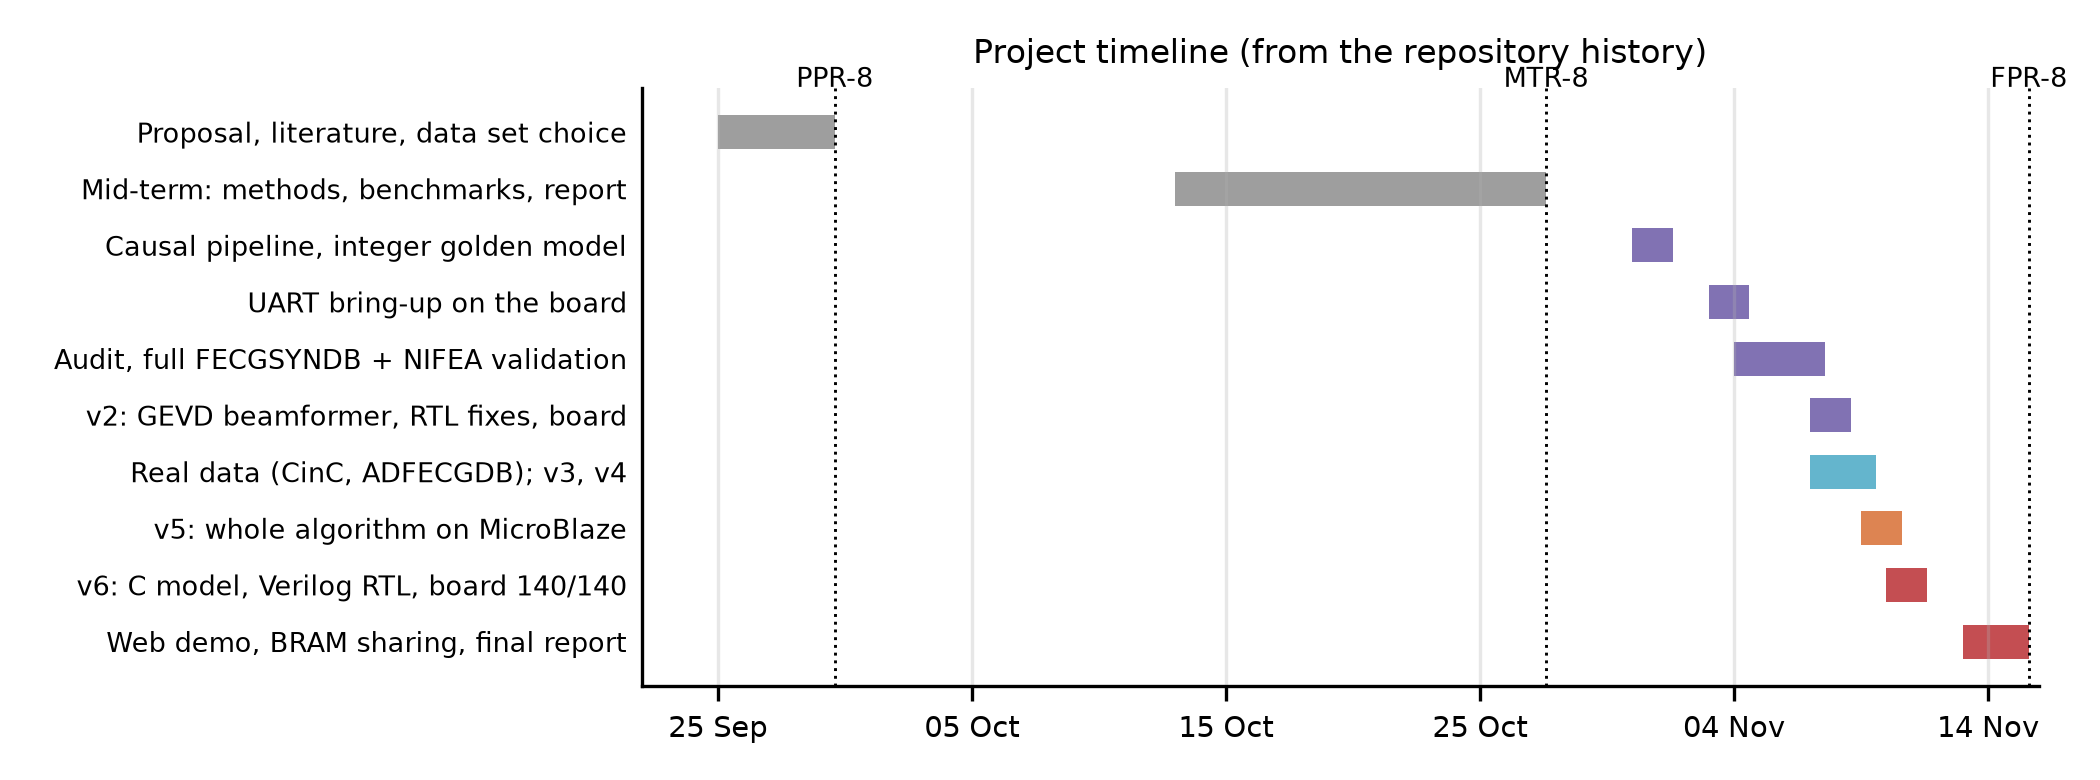
\includegraphics[width=0.72\textwidth]{figures/fin_timeline.png}
\caption{\fb Project timeline from the repository history: preliminary proposal (PPR-8), mid-term report (MTR-8), and the final phase from the causal pipeline to the final RTL design, demonstration and this report (FPR-8).}
\label{fig:fin_project_timeline}
\end{figure*}

\begin{table*}[t]
\fb
\caption{\fb Work division over the whole project. Each member was responsible for one mid-term method and one part of the final system.}
\label{tab:contrib}
\centering
\resizebox{\textwidth}{!}{%
\begin{tabular}{@{}lp{3.1cm}p{6.6cm}p{5.2cm}@{}}
\toprule
\textbf{Member} & \textbf{Part} & \textbf{Main tasks} & \textbf{Key results} \\
\midrule
\textbf{Naman} & Data, test set-up and integration & SVD extraction (3 variants) for the mid-term comparison; data set preparation for FECGSYNDB, CinC 2013, ADFECGDB and NIFEA (loading, unit conversion, annotations); shared mixture builder and test cases TC1--TC5; \texttt{src/fecg} package and test suite, extended with tests for v6.1 and v7 (board match, causality, delay bound); live web demonstration and its v7 view (final and live FHR); assembly of the mid-term and final reports & 270-test suite; common data and test basis used by all members; web page streaming any recording to the board (Sec.~\ref{sec:final_demo}) \\
\midrule
\textbf{Vivek} & Fixed-point design and first full FPGA version & Wavelet-threshold hybrid and SVD-template methods (mid-term); first fixed-point model, test vectors and FPGA feasibility study; UART bring-up on the Spartan-7 and the PC--FPGA message protocol; v5: algorithm ported to C on the MicroBlaze, memory fitting and speed-up; board evaluation script with bit-exact check, its FLUSH/OUT7 extension and the board runs of v6.1 and v7-DL & UART at 921,600 baud; v5 on the board, $3.5\times$ faster after optimisation; v5, v6.1 and v7-DL bit-exact on 140 records \\
\midrule
\textbf{Anshu} & Real-time algorithm and accuracy & Maternal template subtraction and multichannel scaling study (mid-term); 1D U-Net baseline and its test on real data; causal label-free algorithm v2--v5 (maternal cancellation, 16 GEVD candidates, trackers, selection); CinC dev/test protocol and corrected scoring; v6.1 ideas (maternal detector, recalibration, selection experiments); look-ahead algorithms v7-LA and v7-DL (window, delay, integer quality) & U-Net $17.7\%$ on real data (why classical); CinC test $16.7 \to 65.5 \to 76.9\%$, ADFECGDB $37.0 \to 96.1\%$ \\
\midrule
\textbf{Astitva} & Final hardware design (v6 RTL) & SWT + LMS + SSNF wavelet hybrid (mid-term); hardware/PC split; bit-accurate integer C model; hand-written Verilog datapath; xsim unit and system testbenches; implementation and board verification; block RAM optimisation; v6.1 recalibration in the RTL; look-ahead unit \texttt{v7\_la} with its area reduction and the display unit & RTL bit-exact in simulation and 140/140 on the board for every version; 50\,MHz, 4--5$\times$ real time; BRAM $99 \to 80\%$; look-ahead unit $13.2\text{k} \to 8.4\text{k}$ LUTs \\
\bottomrule
\end{tabular}%
}
\end{table*}
\end{finalpart}

% =====================================================================
{\small
\begin{thebibliography}{40}\setlength{\itemsep}{0.5pt}\setlength{\parskip}{0pt}

\bibitem{hasan2009}
M.~A. Hasan, M.~B.~I. Reaz, M.~I. Ibrahimy, M.~S. Hussain, and J.~Uddin.
\newblock Detection and processing techniques of FECG signal for fetal monitoring.
\newblock {\em Biol.\ Procedures Online}, 11(1):263--295, 2009. \url{https://doi.org/10.1186/1477-3155-7-3}

\bibitem{sameni2010}
R.~Sameni and G.~D. Clifford.
\newblock A review of fetal ECG signal processing; issues and promising directions.
\newblock {\em The Open Pacing, Electrophysiology \& Therapy Journal}, 3:4--20, 2010. \url{https://doi.org/10.2174/1876536X01003010004}

\bibitem{clifford2014}
G.~D. Clifford, I.~Silva, J.~Behar, and G.~Moody.
\newblock Non-invasive fetal ECG analysis.
\newblock {\em Physiological Measurement}, 35(8):1521--1536, 2014. \url{https://doi.org/10.1088/0967-3334/35/8/1521}

\bibitem{behar2014}
J.~Behar, A.~Johnson, G.~D. Clifford, and J.~Oster.
\newblock A comparison of single-channel fetal ECG extraction methods.
\newblock {\em Annals of Biomedical Engineering}, 42(6):1340--1353, 2014. \url{https://doi.org/10.1007/s10439-014-0993-9}

\bibitem{behar2014b}
\fin{J.~Behar, J.~Oster, and G.~D. Clifford.
\newblock Combining and benchmarking methods of foetal ECG extraction without maternal or scalp electrode data.
\newblock {\em Physiological Measurement}, 35(8):1569--1589, 2014. \url{https://doi.org/10.1088/0967-3334/35/8/1569}}

\bibitem{andreotti2014}
\fin{F.~Andreotti, M.~Riedl, T.~Himmelsbach, D.~Wedekind, N.~Wessel, H.~Stepan, C.~Schmieder, A.~Jank, H.~Malberg, and S.~Zaunseder.
\newblock Robust fetal ECG extraction and detection from abdominal leads.
\newblock {\em Physiological Measurement}, 35(8):1551--1567, 2014. \url{https://doi.org/10.1088/0967-3334/35/8/1551}}

\bibitem{jaeger2024}
\fin{K.~M. Jaeger, M.~Nissen, S.~Rahm, A.~Titzmann, P.~A. Fasching, J.~Beilner, B.~M. Eskofier, and H.~Leutheuser.
\newblock Power-MF: robust fetal QRS detection from non-invasive fetal electrocardiogram recordings.
\newblock {\em Physiological Measurement}, 45(5):055009, 2024. \url{https://doi.org/10.1088/1361-6579/ad4952}}

\bibitem{zhong2019}
\fin{W.~Zhong, X.~Guo, and G.~Wang.
\newblock QRStree: A prefix tree-based model to fetal QRS complexes detection.
\newblock {\em PLoS ONE}, 14(10):e0223057, 2019. \url{https://doi.org/10.1371/journal.pone.0223057}}

\bibitem{asadi2026}
\fin{A.~Asadi and A.~Ghaffari.
\newblock SCTD-ICA: an ICA-based approach for fetal ECG extraction from single channel abdominal ECG.
\newblock {\em IEEE Journal of Biomedical and Health Informatics}, 30(4):3568--3578, 2026. \url{https://doi.org/10.1109/JBHI.2025.3609696}}

\bibitem{shokouhmand2023}
\fin{A.~Shokouhmand and N.~Tavassolian.
\newblock Fetal electrocardiogram extraction using dual-path source separation of single-channel non-invasive abdominal recordings.
\newblock {\em IEEE Transactions on Biomedical Engineering}, 70(1):283--295, 2023. \url{https://doi.org/10.1109/TBME.2022.3189617}}

\bibitem{abel2023}
J.~D.~K. Abel, S.~Dhanalakshmi, and R.~Kumar.
\newblock A comprehensive survey on signal processing and machine learning techniques for non-invasive fetal ECG extraction.
\newblock {\em Multimedia Tools and Applications}, 82:1373--1400, 2023. \url{https://doi.org/10.1007/s11042-022-13391-0}

\bibitem{sornmo_ecg}
L.~S{\"o}rnmo and P.~Laguna.
\newblock Electrocardiogram (ECG) signal processing.
\newblock In {\em Wiley Encyclopedia of Biomedical Engineering}, 2006. \url{https://doi.org/10.1002/9780471740360.ebs1482}

\bibitem{widrow1975}
B.~Widrow, J.~R. Glover, J.~M. McCool, {\em et al.}
\newblock Adaptive noise cancelling: Principles and applications.
\newblock {\em Proceedings of the IEEE}, 63(12):1692--1716, 1975. \url{https://doi.org/10.1109/PROC.1975.10036}

\bibitem{cerutti1986}
S.~Cerutti, G.~Baselli, S.~Civardi, and E.~Ferrazzi.
\newblock Variability analysis of fetal heart rate signals as obtained from abdominal electrocardiographic recordings.
\newblock {\em J. Perinatal Medicine}, 14(6):445--452, 1986. \url{https://doi.org/10.1515/jpme.1986.14.6.445}

\bibitem{callaerts1990}
D.~Callaerts, B.~De~Moor, J.~Vandewalle, and W.~Sansen.
\newblock Comparison of SVD methods to extract the fetal electrocardiogram from cutaneous electrode signals.
\newblock {\em Medical and Biological Engineering and Computing}, 28(3):217--224, 1990. \url{https://doi.org/10.1007/BF02442682}

\bibitem{kanjilal1997}
P.~P. Kanjilal, S.~Palit, and G.~Saha.
\newblock Fetal ECG extraction from single-channel maternal ECG using singular value decomposition.
\newblock {\em IEEE Transactions on Biomedical Engineering}, 44(1):51--59, 1997. \url{https://doi.org/10.1109/10.553712}

\bibitem{delathauwer2000}
L.~De~Lathauwer, B.~De~Moor, and J.~Vandewalle.
\newblock Fetal electrocardiogram extraction by blind source subspace separation.
\newblock {\em IEEE Transactions on Biomedical Engineering}, 47(5):567--572, 2000. \url{https://doi.org/10.1109/10.841333}

\bibitem{sameni2007}
R.~Sameni, M.~B. Shamsollahi, C.~Jutten, and G.~D. Clifford.
\newblock A nonlinear Bayesian filtering framework for ECG denoising.
\newblock {\em IEEE Transactions on Biomedical Engineering}, 54(12):2172--2185, 2007. \url{https://doi.org/10.1109/TBME.2007.897817}

\bibitem{cardoso1999}
J.-F. Cardoso.
\newblock High-order contrasts for independent component analysis.
\newblock {\em Neural Computation}, 11(1):157--192, 1999. \url{https://doi.org/10.1162/089976699300016863}

\bibitem{hyvarinen2000}
A.~Hyv{\"a}rinen and E.~Oja.
\newblock Independent component analysis: algorithms and applications.
\newblock {\em Neural Networks}, 13(4-5):411--430, 2000. \url{https://doi.org/10.1016/S0893-6080(00)00026-5}

\bibitem{fecgsyndb}
Fetal ECG synthetic database (FECGSYNDB).
\newblock PhysioNet. \url{https://physionet.org/content/fecgsyndb/1.0.0/}, 2016.

\bibitem{andreotti2016}
F.~Andreotti, J.~Behar, F.~Zaunseder, J.~Oster, and G.~D. Clifford.
\newblock An open-source framework for stress-testing non-invasive fetal ECG extraction algorithms.
\newblock {\em Physiological Measurement}, 37(5):627--648, 2016. \url{https://doi.org/10.1088/0967-3334/37/5/627}

\bibitem{nifeadb}
Non-invasive fetal ECG arrhythmia database (NIFEADB).
\newblock PhysioNet. \url{https://physionet.org/content/nifeadb/1.0.0/}, 2016.

\bibitem{ronneberger2015}
O.~Ronneberger, P.~Fischer, and T.~Brox.
\newblock U-Net: Convolutional networks for biomedical image segmentation.
\newblock In {\em MICCAI}, pages 234--241, 2015. \url{https://doi.org/10.1007/978-3-319-24574-4_28}

\bibitem{ahlstrom1985}
M.~L. Ahlstrom and W.~J. Tompkins.
\newblock Digital filters for real-time ECG signal processing using microprocessors.
\newblock {\em IEEE Transactions on Biomedical Engineering}, BME-32(9):708--713, 1985. \url{https://doi.org/10.1109/TBME.1985.325585}

\bibitem{xilinx_dsp48}
Xilinx.
\newblock {\em 7 Series DSP48E1 Slice User Guide (UG479)}.
\newblock Xilinx, San Jose, CA, v1.10 edition, 2018.

\bibitem{constantinides2004}
G.~A. Constantinides, P.~Y.~K. Cheung, and W.~Luk.
\newblock Wordlength optimization for linear digital signal processing.
\newblock {\em IEEE Transactions on Computer-Aided Design of Integrated Circuits and Systems}, 22(10):1432--1442, 2003. \url{https://doi.org/10.1109/TCAD.2003.818119}

\bibitem{pan1985}
J.~Pan and W.~J. Tompkins.
\newblock A real-time QRS detection algorithm.
\newblock {\em IEEE Transactions on Biomedical Engineering}, BME-32(3):230--236, 1985. \url{https://doi.org/10.1109/TBME.1985.325532}

\bibitem{silva2013}
I.~Silva, J.~Behar, R.~Sameni, T.~Zhu, J.~Oster, G.~D. Clifford, and G.~B. Moody.
\newblock Noninvasive fetal ECG: the PhysioNet/Computing in Cardiology Challenge 2013.
\newblock {\em Computing in Cardiology}, 40:149--152, 2013. \url{https://www.cinc.org/archives/2013/pdf/0149.pdf}

\bibitem{realdigital_boolean}
RealDigital.
\newblock {\em Boolean Board Reference Manual: Spartan-7 XC7S50 FPGA Platform}.
\newblock RealDigital Inc., 2023. \url{https://www.realdigital.org/hardware/boolean}

\bibitem{edwin2022}
D.~Edwin~Dhas and M.~Suchetha.
\newblock Hardware-efficient neural-coprocessor-based adaptive filtering for real-time fetal ECG extraction on FPGA.
\newblock {\em IEEE Transactions on Biomedical Circuits and Systems}, 16(5):981--990, 2022. \url{https://doi.org/10.1109/TBCAS.2022.3204439}

\bibitem{pani2016}
D.~Pani, G.~Barabino, and L.~Raffo.
\newblock Real-time embedded JADE for fetal electrocardiogram extraction.
\newblock {\em Biomedical Signal Processing and Control}, 27:84--95, 2016. \url{https://doi.org/10.1016/j.bspc.2016.02.001}

\bibitem{anthropic2024}
Anthropic.
\newblock The Claude 3.5 Sonnet language model.
\newblock Large language model system, 2024. \url{https://www.anthropic.com/claude}

\bibitem{openai2024}
OpenAI.
\newblock GPT-4o system card.
\newblock Technical report, OpenAI, 2024. \url{https://openai.com/index/gpt-4o-system-card}

{\color{finalblue}
\bibitem{goldberger2000}
A.~L. Goldberger, L.~A.~N. Amaral, L.~Glass, J.~M. Hausdorff, P.~Ch. Ivanov, R.~G. Mark, J.~E. Mietus, G.~B. Moody, C.-K. Peng, and H.~E. Stanley.
\newblock PhysioBank, PhysioToolkit, and PhysioNet: components of a new research resource for complex physiologic signals.
\newblock {\em Circulation}, 101(23):e215--e220, 2000. \url{https://doi.org/10.1161/01.CIR.101.23.e215}

\bibitem{jezewski2012}
J.~Jezewski, A.~Matonia, T.~Kupka, D.~Roj, and R.~Czabanski.
\newblock Determination of fetal heart rate from abdominal signals: evaluation of beat-to-beat accuracy in relation to the direct fetal electrocardiogram.
\newblock {\em Biomedical Engineering / Biomedizinische Technik}, 57(5):383--394, 2012. \url{https://doi.org/10.1515/bmt-2011-0130}

\bibitem{sameni2008}
R.~Sameni, C.~Jutten, and M.~B. Shamsollahi.
\newblock Multichannel electrocardiogram decomposition using periodic component analysis.
\newblock {\em IEEE Transactions on Biomedical Engineering}, 55(8):1935--1940, 2008. \url{https://doi.org/10.1109/TBME.2008.919714}

\bibitem{claudecode}
Anthropic.
\newblock Claude Code (AI coding assistant), used with the Claude Opus 5.5 model, November 2026.
\newblock \url{https://www.anthropic.com/claude-code}

}
\end{thebibliography}
}

\end{document}
